\documentclass{report}

%%%%%%%%%%%%%%%%%%%%%%%%%%%%%%%%%
% PACKAGE IMPORTS
%%%%%%%%%%%%%%%%%%%%%%%%%%%%%%%%%


\usepackage[tmargin=2cm,rmargin=1in,lmargin=1in,margin=0.85in,bmargin=1.5cm,footskip=.2in]{geometry}
\usepackage{amsmath,amsfonts,amsthm,amssymb,mathtools}

% \usepackage[bb=dsserif]{mathalpha}
% \usepackage{bm}
\usepackage{dsfont}
\usepackage{bookmark} 
\usepackage{booktabs}
\usepackage{enumerate}
\usepackage[shortlabels]{enumitem}
\usepackage{hyperref,theoremref}
\usepackage[table]{xcolor}
\usepackage[most,many,breakable]{tcolorbox}
\usepackage{xcolor}
\usepackage{graphicx}
\graphicspath{ {./images/} }
\usepackage{varwidth}
\usepackage{varwidth}
\usepackage{etoolbox}
%\usepackage{authblk}
\usepackage{nameref}
\usepackage{multicol,array}
\usepackage{tikz-cd}
\usepackage{cancel}
\usepackage{pgfplots}
\pgfplotsset{compat=newest}
\usepgfplotslibrary{patchplots}
\usepackage{anyfontsize}
\usepackage{sectsty}
%\usepackage{import}
%\usepackage{xifthen}
%\usepackage{pdfpages}
%\usepackage{transparent}
\usepackage[nameinlink]{cleveref}
\usepackage{fancyhdr}


%%%%%%%%%%%%%%%%%%%%%%%%%%%%%%
% HEADER AND FOOTER
%%%%%%%%%%%%%%%%%%%%%%%%%%%%%%
\pagestyle{fancy}

% Clear all header and footer fields
\fancyhf{}

% Redefine the chaptermark
\renewcommand{\chaptermark}[1]{%
  \markboth{\thechapter.\ \MakeUppercase{#1}}{}%
}

% Chapter name on the left of the header
\fancyhead[L]{\leftmark}

% Section name on the right of the header
\fancyhead[R]{\rightmark}

% Page number on the bottom right in the format "- 34 -"
\fancyhead[C]{\raisebox{-0pt}{-\hspace{4pt}\thepage\hspace{4pt}-}}

% Line at the top of the header
\renewcommand{\headrulewidth}{0.0pt}

\fancypagestyle{plain}{%
  \fancyhf{} % clear all header and footer fields
  \renewcommand{\headrulewidth}{0pt} % remove the header rule
  \renewcommand{\footrulewidth}{0pt} % remove the footer rule
}
%%%%%%%%%%%%%%%%%%%%%%%%%%%%%%
% SELF MADE COLORS
%%%%%%%%%%%%%%%%%%%%%%%%%%%%%%

\usetikzlibrary{shapes.geometric}
\usetikzlibrary{calc}
\usepackage{anyfontsize}

\definecolor{myg}{RGB}{56, 140, 70}
\definecolor{myb}{RGB}{45, 111, 177}
\definecolor{myr}{RGB}{199, 68, 64}
\definecolor{mytheorembg}{HTML}{fdf8ea} %orange
\definecolor{mytheoremfr}{HTML}{f19000}
\definecolor{myexamplebg}{HTML}{F2FBF8}
\definecolor{myexamplefr}{HTML}{88D6D1}
\definecolor{myexampleti}{HTML}{2A7F7F}
\definecolor{mydefinitbg}{HTML}{F2F2F9} %blue
\definecolor{mydefinitfr}{HTML}{00007B} 
\definecolor{mypropbg}{RGB}{56, 140, 70} %green
\definecolor{mypropfr}{RGB}{56, 140, 70}
\definecolor{mylemmabg}{RGB}{169, 144, 126}
\definecolor{mylemmafr}{RGB}{169, 144, 126}
\definecolor{notesgreen}{RGB}{0,162,0}
\definecolor{myp}{RGB}{197, 92, 212}
\definecolor{mygr}{HTML}{2C3338}
\definecolor{myred}{RGB}{127,0,0}
\definecolor{myyellow}{RGB}{169,121,69}
\definecolor{OrangeRed}{HTML}{ED135A}
\definecolor{Dandelion}{HTML}{FDBC42}
\definecolor{light-gray}{gray}{0.95}
\definecolor{Emerald}{HTML}{00A99D}
\definecolor{RoyalBlue}{HTML}{0071BC}

% \definecolor{mydefnewbg}{HTML}{FFF0E0}
% \definecolor{mydefnewfr}{HTML}{FF9900}
\definecolor{myRoyalBlue}{RGB}{50,60,150}
\definecolor{myGreen}{RGB}{45,100,45}
\definecolor{mynavy}{RGB}{56, 102, 148} % RGB color model

%%%%%%%%%%%%%%%%%%%%%%%%%%%%%%
% HYPERREF SETUP
%%%%%%%%%%%%%%%%%%%%%%%%%%%%%%

\hypersetup{
	colorlinks=true,
	linkcolor=mynavy,
	citecolor=BurntOrange,
	bookmarksnumbered=true,
	bookmarksopen=true,
}

%%%%%%%%%%%%%%%%%%%%%%%%%%%%
% TCOLORBOX SETUPS
%%%%%%%%%%%%%%%%%%%%%%%%%%%%


%================================
% NEW DEFINITION BOX
%================================


\newtcbtheorem[number within=section]{definition}{Definition}
{%
    enhanced
    ,breakable
    ,colback = mydefinitbg
    ,frame hidden
    ,boxrule = 0sp
    ,borderline west = {2pt}{0pt}{mydefinitfr}
    ,sharp corners
    ,detach title
    ,before upper = \tcbtitle\par\smallskip
    ,coltitle = mydefinitfr!85!black
    ,fonttitle = \bfseries\sffamily
    ,description font = \mdseries
    ,separator sign none
    ,segmentation style={solid, mydefinitfr!85!black}
	,label type=definition
}
{th}

% \newtcbtheorem[number within=chapter]{definition}{Definition}
% {%
%     enhanced
%     ,breakable
%     ,colback = mydefinitbg
%     ,frame hidden
%     ,boxrule = 0sp
%     ,borderline west = {2pt}{0pt}{mydefinitfr}
%     ,sharp corners
%     ,detach title
%     ,before upper = \tcbtitle\par\smallskip
%     ,coltitle = mydefinitfr!85!black
%     ,fonttitle = \bfseries\sffamily
%     ,description font = \mdseries
%     ,separator sign none
%     ,segmentation style={solid, mydefinitfr!85!black}
% 	,label type=definition
% }
% {th}

\setlength{\parindent}{0.5cm}
%================================
% THEOREM BOX
%================================

\tcbuselibrary{theorems,skins,hooks}
\newtcbtheorem[use counter from=definition, number within=section]{theorem}{Theorem}
{%
	enhanced,
	breakable,
	colback = mytheorembg,
	frame hidden,
	boxrule = 0sp,
	borderline west = {2pt}{0pt}{mytheoremfr},
	sharp corners,
	detach title,
	before upper = \tcbtitle\par\smallskip,
	coltitle = mytheoremfr,
	fonttitle = \bfseries\sffamily,
	description font = \mdseries,
	separator sign none,
	segmentation style={solid, mytheoremfr},
	label type=theorem
}
{th}

% \tcbuselibrary{theorems,skins,hooks}
% \newtcbtheorem[number within=chapter]{theorem}{Theorem}
% {%
% 	enhanced,
% 	breakable,
% 	colback = mytheorembg,
% 	frame hidden,
% 	boxrule = 0sp,
% 	borderline west = {2pt}{0pt}{mytheoremfr},
% 	sharp corners,
% 	detach title,
% 	before upper = \tcbtitle\par\smallskip,
% 	coltitle = mytheoremfr,
% 	fonttitle = \bfseries\sffamily,
% 	description font = \mdseries,
% 	separator sign none,
% 	segmentation style={solid, mytheoremfr},
% 	label type=theorem
% }
% {th}


\tcbuselibrary{theorems,skins,hooks}
\newtcolorbox{Theoremcon}
{%
	enhanced
	,breakable
	,colback = mytheorembg
	,frame hidden
	,boxrule = 0sp
	,borderline west = {2pt}{0pt}{mytheoremfr}
	,sharp corners
	,description font = \mdseries
	,separator sign none
}


%================================
% Corollery
%================================
\tcbuselibrary{theorems,skins,hooks}
\newtcbtheorem[use counter from=definition, number within=section]{corollary}{Corollary}
{%
	enhanced
	,breakable
	,colback = myp!10
	,frame hidden
	,boxrule = 0sp
	,borderline west = {2pt}{0pt}{myp!85!black}
	,sharp corners
	,detach title
	,before upper = \tcbtitle\par\smallskip
	,coltitle = myp!85!black
	,fonttitle = \bfseries\sffamily
	,description font = \mdseries
	,separator sign none
	,segmentation style={solid, myp!85!black}
	,label type=corollary
}
{th}
% \tcbuselibrary{theorems,skins,hooks}
% \newtcbtheorem[number within=chapter]{corollary}{Corollary}
% {%
% 	enhanced
% 	,breakable
% 	,colback = myp!10
% 	,frame hidden
% 	,boxrule = 0sp
% 	,borderline west = {2pt}{0pt}{myp!85!black}
% 	,sharp corners
% 	,detach title
% 	,before upper = \tcbtitle\par\smallskip
% 	,coltitle = myp!85!black
% 	,fonttitle = \bfseries\sffamily
% 	,description font = \mdseries
% 	,separator sign none
% 	,segmentation style={solid, myp!85!black}
% 	,label type=corol
% }
% {th}

%================================
% CLAIM
%================================

\tcbuselibrary{theorems,skins,hooks}
\newtcbtheorem[number within=section]{claim}{Claim}
{%
	enhanced
	,breakable
	,colback = myg!10
	,frame hidden
	,boxrule = 0sp
	,borderline west = {2pt}{0pt}{myg}
	,sharp corners
	,detach title
	,before upper = \tcbtitle\par\smallskip
	,coltitle = myg!85!black
	,fonttitle = \bfseries\sffamily
	,description font = \mdseries
	,separator sign none
	,segmentation style={solid, myg!85!black}
	,label type=claim
}
{th}


\newtcbtheorem[number within=chapter]{Claim}{Claim}
{%
	enhanced
	,breakable
	,colback = myg!10
	,frame hidden
	,boxrule = 0sp
	,borderline west = {2pt}{0pt}{myg}
	,sharp corners
	,detach title
	,before upper = \tcbtitle\par\smallskip
	,coltitle = myg!85!black
	,fonttitle = \bfseries\sffamily
	,description font = \mdseries
	,separator sign none
	,segmentation style={solid, myg!85!black}
	,label type=claim
}
{th}
%================================
% PROPOSITION
%================================

\tcbuselibrary{theorems,skins,hooks}
\newtcbtheorem[use counter from=definition, number within=section]{proposition}{Proposition}
{%
	enhanced
	,breakable
	,colback = mypropbg!10
	,frame hidden
	,boxrule = 0sp
	,borderline west = {2pt}{0pt}{mypropfr!85!black}
	,sharp corners
	,detach title
	,before upper = \tcbtitle\par\smallskip
	,coltitle = mypropfr!85!black
	,fonttitle = \bfseries\sffamily
	,description font = \mdseries
	,separator sign none
	,segmentation style={solid, mypropfr!85!black}
	,label type=proposition
}
{th}

% \newtcbtheorem[number within=chapter]{Proposition}{Proposition}
% {%
% 	enhanced
% 	,breakable
% 	,colback = mypropbg!10
% 	,frame hidden
% 	,boxrule = 0sp
% 	,borderline west = {2pt}{0pt}{mypropfr!85!black}
% 	,sharp corners
% 	,detach title
% 	,before upper = \tcbtitle\par\smallskip
% 	,coltitle = mypropfr!85!black
% 	,fonttitle = \bfseries\sffamily
% 	,description font = \mdseries
% 	,separator sign none
% 	,segmentation style={solid, mypropfr!85!black}
% 	,label type=proposition
% }
% {th}
%================================
% LEMMA
%================================

\tcbuselibrary{theorems,skins,hooks}
\newtcbtheorem[use counter from=definition, number within=section]{lemma}{Lemma}
{%
	enhanced
	,breakable
	,colback = mylemmabg!10
	,frame hidden
	,boxrule = 0sp
	,borderline west = {2pt}{0pt}{mylemmafr!85!black}
	,sharp corners
	,detach title
	,before upper = \tcbtitle\par\smallskip
	,coltitle = mylemmafr!85!black
	,fonttitle = \bfseries\sffamily
	,description font = \mdseries
	,separator sign none
	,segmentation style={solid, mylemmafr!85!black}
	,label type=lemma
}
{th}

% \newtcbtheorem[number within=chapter]{Lemma}{Lemma}
% {%
% 	enhanced
% 	,breakable
% 	,colback = mylemmabg!10
% 	,frame hidden
% 	,boxrule = 0sp
% 	,borderline west = {2pt}{0pt}{mylemmafr!85!black}
% 	,sharp corners
% 	,detach title
% 	,before upper = \tcbtitle\par\smallskip
% 	,coltitle = mylemmafr!85!black
% 	,fonttitle = \bfseries\sffamily
% 	,description font = \mdseries
% 	,separator sign none
% 	,segmentation style={solid, mylemmafr!85!black}
% 	,label type=lemma
% }
% {th}
%================================
% EXAMPLE BOX
%================================

\newtcbtheorem[number within=section]{example}{Example}
{%
	colback = myexamplebg
	,breakable
	,colframe = myexamplefr
	,coltitle = myexampleti
	,boxrule = 1pt
	,sharp corners
	,detach title
	,before upper=\tcbtitle\par\smallskip
	,fonttitle = \bfseries\sffamily
	%,fonttitle = \bfseries
	,description font = \mdseries\sffamily
	%,description font = \mdseries
	,separator sign none
	%,description delimiters parenthesis
	,label type=example
}
{ex}

% \newtcbtheorem[number within=chapter]{example}{Example}
% {%
% 	colback = myexamplebg
% 	,breakable
% 	,colframe = myexamplefr
% 	,coltitle = myexampleti
% 	,boxrule = 1pt
% 	,sharp corners
% 	,detach title
% 	,before upper=\tcbtitle\par\smallskip
% 	,fonttitle = \bfseries
% 	,description font = \mdseries
% 	,separator sign none
% 	,description delimiters parenthesis
% 	,label type=example
% }
% {ex}

%================================
% DEFINITION BOX
%================================

% \newtcbtheorem[number within=section]{Definition}{Definition}{enhanced,
% 	before skip=2mm,after skip=2mm, colback=red!5,colframe=red!80!black,boxrule=0.5mm,
% 	attach boxed title to top left={xshift=1cm,yshift*=1mm-\tcboxedtitleheight}, varwidth boxed title*=-3cm,
% 	boxed title style={frame code={
% 					\path[fill=tcbcolback]
% 					([yshift=-1mm,xshift=-1mm]frame.north west)
% 					arc[start angle=0,end angle=180,radius=1mm]
% 					([yshift=-1mm,xshift=1mm]frame.north east)
% 					arc[start angle=180,end angle=0,radius=1mm];
% 					\path[left color=tcbcolback!60!black,right color=tcbcolback!60!black,
% 						middle color=tcbcolback!80!black]
% 					([xshift=-2mm]frame.north west) -- ([xshift=2mm]frame.north east)
% 					[rounded corners=1mm]-- ([xshift=1mm,yshift=-1mm]frame.north east)
% 					-- (frame.south east) -- (frame.south west)
% 					-- ([xshift=-1mm,yshift=-1mm]frame.north west)
% 					[sharp corners]-- cycle;
% 				},interior engine=empty,
% 		},
% 	fonttitle=\bfseries,
% 	title={#2},#1}{def}
% \newtcbtheorem[number within=chapter]{definition}{Definition}{enhanced,
% 	before skip=2mm,after skip=2mm, colback=red!5,colframe=red!80!black,boxrule=0.5mm,
% 	attach boxed title to top left={xshift=1cm,yshift*=1mm-\tcboxedtitleheight}, varwidth boxed title*=-3cm,
% 	boxed title style={frame code={
% 					\path[fill=tcbcolback]
% 					([yshift=-1mm,xshift=-1mm]frame.north west)
% 					arc[start angle=0,end angle=180,radius=1mm]
% 					([yshift=-1mm,xshift=1mm]frame.north east)
% 					arc[start angle=180,end angle=0,radius=1mm];
% 					\path[left color=tcbcolback!60!black,right color=tcbcolback!60!black,
% 						middle color=tcbcolback!80!black]
% 					([xshift=-2mm]frame.north west) -- ([xshift=2mm]frame.north east)
% 					[rounded corners=1mm]-- ([xshift=1mm,yshift=-1mm]frame.north east)
% 					-- (frame.south east) -- (frame.south west)
% 					-- ([xshift=-1mm,yshift=-1mm]frame.north west)
% 					[sharp corners]-- cycle;
% 				},interior engine=empty,
% 		},
% 	fonttitle=\bfseries,
% 	title={#2},#1}{def}



%================================
% OPEN QUESTION BOX
%================================

\newtcbtheorem[number within=section]{open}{Open Question}{enhanced,
	before skip=2mm,after skip=2mm, colback=myp!5,colframe=myp!80!black,boxrule=0.5mm,
	attach boxed title to top left={xshift=1cm,yshift*=1mm-\tcboxedtitleheight}, varwidth boxed title*=-3cm,
	boxed title style={frame code={
			\path[fill=tcbcolback]
			([yshift=-1mm,xshift=-1mm]frame.north west)
			arc[start angle=0,end angle=180,radius=1mm]
			([yshift=-1mm,xshift=1mm]frame.north east)
			arc[start angle=180,end angle=0,radius=1mm];
			\path[left color=tcbcolback!60!black,right color=tcbcolback!60!black,
			middle color=tcbcolback!80!black]
			([xshift=-2mm]frame.north west) -- ([xshift=2mm]frame.north east)
			[rounded corners=1mm]-- ([xshift=1mm,yshift=-1mm]frame.north east)
			-- (frame.south east) -- (frame.south west)
			-- ([xshift=-1mm,yshift=-1mm]frame.north west)
			[sharp corners]-- cycle;
		},interior engine=empty,
	},
	fonttitle=\bfseries,
	title={#2},#1}{def}
\newtcbtheorem[number within=chapter]{Open}{Open Question}{enhanced,
	before skip=2mm,after skip=2mm, colback=myp!5,colframe=myp!80!black,boxrule=0.5mm,
	attach boxed title to top left={xshift=1cm,yshift*=1mm-\tcboxedtitleheight}, varwidth boxed title*=-3cm,
	boxed title style={frame code={
			\path[fill=tcbcolback]
			([yshift=-1mm,xshift=-1mm]frame.north west)
			arc[start angle=0,end angle=180,radius=1mm]
			([yshift=-1mm,xshift=1mm]frame.north east)
			arc[start angle=180,end angle=0,radius=1mm];
			\path[left color=tcbcolback!60!black,right color=tcbcolback!60!black,
			middle color=tcbcolback!80!black]
			([xshift=-2mm]frame.north west) -- ([xshift=2mm]frame.north east)
			[rounded corners=1mm]-- ([xshift=1mm,yshift=-1mm]frame.north east)
			-- (frame.south east) -- (frame.south west)
			-- ([xshift=-1mm,yshift=-1mm]frame.north west)
			[sharp corners]-- cycle;
		},interior engine=empty,
	},
	fonttitle=\bfseries,
	title={#2},#1}{def}



%================================
% EXERCISE BOX
%================================

\makeatletter
\newtcbtheorem{question}{Question}{enhanced,
	breakable,
	colback=white,
	colframe=myb!80!black,
	attach boxed title to top left={yshift*=-\tcboxedtitleheight},
	fonttitle=\bfseries,
	title={#2},
	boxed title size=title,
	boxed title style={%
			sharp corners,
			rounded corners=northwest,
			colback=tcbcolframe,
			boxrule=0pt,
		},
	underlay boxed title={%
			\path[fill=tcbcolframe] (title.south west)--(title.south east)
			to[out=0, in=180] ([xshift=5mm]title.east)--
			(title.center-|frame.east)
			[rounded corners=\kvtcb@arc] |-
			(frame.north) -| cycle;
		},
	#1
}{def}
\makeatother

%================================
% SOLUTION BOX
%================================

\makeatletter
\newtcolorbox{solution}{enhanced,
	breakable,
	colback=white,
	colframe=myg!80!black,
	attach boxed title to top left={yshift*=-\tcboxedtitleheight},
	title=Solution,
	boxed title size=title,
	boxed title style={%
			sharp corners,
			rounded corners=northwest,
			colback=tcbcolframe,
			boxrule=0pt,
		},
	underlay boxed title={%
			\path[fill=tcbcolframe] (title.south west)--(title.south east)
			to[out=0, in=180] ([xshift=5mm]title.east)--
			(title.center-|frame.east)
			[rounded corners=\kvtcb@arc] |-
			(frame.north) -| cycle;
		},
}
\makeatother

%================================
% Question BOX
%================================

\makeatletter
\newtcbtheorem{qstion}{Question}{enhanced,
	breakable,
	colback=white,
	colframe=mygr,
	attach boxed title to top left={yshift*=-\tcboxedtitleheight},
	fonttitle=\bfseries,
	title={#2},
	boxed title size=title,
	boxed title style={%
			sharp corners,
			rounded corners=northwest,
			colback=tcbcolframe,
			boxrule=0pt,
		},
	underlay boxed title={%
			\path[fill=tcbcolframe] (title.south west)--(title.south east)
			to[out=0, in=180] ([xshift=5mm]title.east)--
			(title.center-|frame.east)
			[rounded corners=\kvtcb@arc] |-
			(frame.north) -| cycle;
		},
	#1
}{def}
\makeatother

\newtcbtheorem[number within=chapter]{wconc}{Wrong Concept}{
	breakable,
	enhanced,
	colback=white,
	colframe=myr,
	arc=0pt,
	outer arc=0pt,
	fonttitle=\bfseries\sffamily\large,
	colbacktitle=myr,
	attach boxed title to top left={},
	boxed title style={
			enhanced,
			skin=enhancedfirst jigsaw,
			arc=3pt,
			bottom=0pt,
			interior style={fill=myr}
		},
	#1
}{def}



%================================
% NOTE BOX
%================================

\usetikzlibrary{arrows,calc,shadows.blur}
\tcbuselibrary{skins}
\newtcolorbox{note}[1][]{%
	enhanced jigsaw,
	colback=gray!20!white,%
	colframe=gray!80!black,
	size=small,
	boxrule=1pt,
	title=\textbf{Note:-},
	halign title=flush center,
	coltitle=black,
	breakable,
	drop shadow=black!50!white,
	attach boxed title to top left={xshift=1cm,yshift=-\tcboxedtitleheight/2,yshifttext=-\tcboxedtitleheight/2},
	minipage boxed title=1.5cm,
	boxed title style={%
			colback=white,
			size=fbox,
			boxrule=1pt,
			boxsep=2pt,
			underlay={%
					\coordinate (dotA) at ($(interior.west) + (-0.5pt,0)$);
					\coordinate (dotB) at ($(interior.east) + (0.5pt,0)$);
					\begin{scope}
						\clip (interior.north west) rectangle ([xshift=3ex]interior.east);
						\filldraw [white, blur shadow={shadow opacity=60, shadow yshift=-.75ex}, rounded corners=2pt] (interior.north west) rectangle (interior.south east);
					\end{scope}
					\begin{scope}[gray!80!black]
						\fill (dotA) circle (2pt);
						\fill (dotB) circle (2pt);
					\end{scope}
				},
		},
	#1,
}

%%%%%%%%%%%%%%%%%%%%%%%%%%%%%%
% SELF MADE COMMANDS
%%%%%%%%%%%%%%%%%%%%%%%%%%%%%%

\NewDocumentCommand{\EqM}{ m O{black} m}{%
	\tikz[remember picture, baseline, anchor=base] 
	\node[inner sep=0pt, outer sep=3pt, text=#2] (#1) {%
		\ensuremath{#3}%
	};    
}

% \newcommand{\thm}[3][]{\begin{theorem}{#2}{#1}#3\end{theorem}}
% \newcommand{\thmc}[3][]{\begin{theorem}{#2}{#1}#3\end{theorem}}
% \newcommand{\cor}[3][]{\begin{corollary}{#2}{#1}#3\end{corollary}}
% \newcommand{\corc}[3][]{\begin{corollary}{#2}{#1}#3\end{corollary}}
% \newcommand{\clm}[3][]{\begin{claim}{#2}{#1}#3\end{claim}}
% \newcommand{\prop}[3][]{\begin{proposition}{#2}{#1}#3\end{proposition}}
% \newcommand{\lemm}[3][]{\begin{lemma}{#2}{#1}#3\end{lemma}}
% \newcommand{\wc}[3][]{\begin{wconc}{#2}{#1}\setlength{\parindent}{1cm}#3\end{wconc}}
% \newcommand{\thmcon}[1]{\begin{Theoremcon}{#1}\end{Theoremcon}}
% \newcommand{\ex}[3][]{\begin{example}{#2}{#1}#3\end{example}}
% \newcommand{\exc}[3][]{\begin{example}{#2}{#1}#3\end{example}}
% \newcommand{\dfn}[3][]{\begin{definition}{#2}{#1}#3\end{definition}}
% \newcommand{\dfn}[3][]{\begin{Definition}[colbacktitle=red!75!black]{#2}{#1}#3\end{Definition}}
% \newcommand{\dfnc}[3][]{\begin{definition}[colbacktitle=red!75!black]{#2}{#1}#3\end{definition}}
% \newcommand{\opn}[3][]{\begin{open}[colbacktitle=myp!75!black]{#2}{#1}#3\end{open}}
% \newcommand{\opnc}[3][]{\begin{Open}[colbacktitle=myp!75!black]{#2}{#1}#3\end{Open}}
% \newcommand{\qs}[3][]{\begin{question}{#2}{#1}#3\end{question}}
%\newcommand{\pf}[2]{\begin{myproof}[#1]#2\end{myproof}}
% \newcommand{\pf}[2][Proof]{\begin{prf}[#1]#2\end{prf}}
% \newcommand{\nt}[1]{\begin{note}#1\end{note}}

\newcommand*\circled[1]{\tikz[baseline=(char.base)]{
		\node[shape=circle,draw,inner sep=1pt] (char) {#1};}}
\newcommand\getcurrentref[1]{%
	\ifnumequal{\value{#1}}{0}
	{??}
	{\the\value{#1}}%
}
\newcommand{\getCurrentSectionNumber}{\getcurrentref{section}}
\newenvironment{prf}[1][\proofname]{%
	\proof[#1.]%
}{\endproof}
\newcounter{mylabelcounter}

\makeatletter
\newcommand{\setword}[2]{%
	\phantomsection
	#1\def\@currentlabel{\unexpanded{#1}}\label{#2}%
}
\makeatother

\newenvironment{remark}[1][Remark]{%
    \par\noindent\textit{#1.}\hspace{1ex}%
}{\qed\par}


\tikzset{
	symbol/.style={
			draw=none,
			every to/.append style={
					edge node={node [sloped, allow upside down, auto=false]{$#1$}}}
		}
}

%\usepackage{framed}
%\usepackage{titletoc}
%\usepackage{etoolbox}
%\usepackage{lmodern}


%\patchcmd{\tableofcontents}{\contentsname}{\sffamily\contentsname}{}{}

%\renewenvironment{leftbar}
%{\def\FrameCommand{\hspace{6em}%
%		{\color{myyellow}\vrule width 2pt depth 6pt}\hspace{1em}}%
%	\MakeFramed{\parshape 1 0cm \dimexpr\textwidth-6em\relax\FrameRestore}\vskip2pt%
%}
%{\endMakeFramed}

%\titlecontents{chapter}
%[0em]{\vspace*{2\baselineskip}}
%{\parbox{4.5em}{%
%		\hfill\Huge\sffamily\bfseries\color{myred}\thecontentspage}%
%	\vspace*{-2.3\baselineskip}\leftbar\textsc{\small\chaptername~\thecontentslabel}\\\sffamily}
%{}{\endleftbar}
%\titlecontents{section}
%[8.4em]
%{\sffamily\contentslabel{3em}}{}{}
%{\hspace{0.5em}\nobreak\itshape\color{myred}\contentspage}
%\titlecontents{subsection}
%[8.4em]
%{\sffamily\contentslabel{3em}}{}{}  
%{\hspace{0.5em}\nobreak\itshape\color{myred}\contentspage}



%%%%%%%%%%%%%%%%%%%%%%%%%%%%%%%%%%%%%%%%%%%
% TABLE OF CONTENTS
%%%%%%%%%%%%%%%%%%%%%%%%%%%%%%%%%%%%%%%%%%%


\usepackage{titletoc}
\usepackage{sectsty} % For customizing section titles if needed

\renewcommand{\contentsname}{\fontfamily{times}\selectfont\Huge\bfseries\sffamily Contents}

% Define custom colors as per tstextbook.cls
\definecolor{tssteelblue}{RGB}{70,130,180}
\definecolor{tsorange}{RGB}{255,138,88}

% Customizing the Table of Contents

\contentsmargin{1cm}

% Chapter titles
\titlecontents{chapter}[0.25cm]
{\addvspace{2ex}\Large\bfseries\sffamily} % Spacing and font adjustments before the entry
{\hypersetup{linkcolor=tssteelblue}\color{tssteelblue}\contentslabel[\Large\thecontentslabel]{1.0cm}} % Label (number) formatting
{\hypersetup{linkcolor=tssteelblue}} % For unnumbered chapters
{\color{tssteelblue}\titlerule*[1pc]{.}\contentspage} % Dot leader and page number

% Section titles
\titlecontents{section}[1.5cm] % Indentation
{\addvspace{0.7ex}\large\bfseries\sffamily} % Spacing and font adjustments before the entry
{\hypersetup{linkcolor=black}\contentslabel[\thecontentslabel]{1.25cm}} % Label (number) formatting
{}
{\sffamily\hfill\color{black}\contentspage}[]

\titlecontents{subsection}[2.65cm] % Adjust the left margin to align with subsection indent
{\addvspace{0.25em}\sffamily}
{\hypersetup{linkcolor=black!85}\contentslabel[\thecontentslabel]{3.2em}} % Subsection label formatting
{} % Unnumbered format
{\hfill\color{black}\contentspage} % Page number


% \usepackage{tikz}
% \definecolor{doc}{RGB}{0,60,110}
% \usepackage{titletoc}
% \contentsmargin{0cm}
% \titlecontents{chapter}[3.7pc]
% {\addvspace{30pt}%
% 	\begin{tikzpicture}[remember picture, overlay]%
% 		\draw[fill=doc!60,draw=doc!60] (-7,-.1) rectangle (-0.7,.5);%
% 		\pgftext[left,x=-3.6cm,y=0.2cm]{\color{white}\Large\sc\bfseries Chapter\ \thecontentslabel};%
% 	\end{tikzpicture}\color{doc!60}\large\sc\bfseries}%
% {}
% {}
% {\;\titlerule\;\large\sc\bfseries Page \thecontentspage
% 	\begin{tikzpicture}[remember picture, overlay]
% 		\draw[fill=doc!60,draw=doc!60] (2pt,0) rectangle (4,0.1pt);
% 	\end{tikzpicture}}%
% \titlecontents{section}[3.7pc]
% {\addvspace{2pt}}
% {\contentslabel[\thecontentslabel]{2pc}}
% {}
% {\hfill\small \thecontentspage}
% []
% \titlecontents*{subsection}[3.7pc]
% {\addvspace{-1pt}\small}
% {}
% {}
% {\ --- \small\thecontentspage}
% [ \textbullet\ ][]

% \makeatletter
% \renewcommand{\tableofcontents}{%
% 	\chapter*{%
% 	  \vspace*{-20\p@}%
% 	  \begin{tikzpicture}[remember picture, overlay]%
% 		  \pgftext[right,x=15cm,y=0.2cm]{\color{doc!60}\Huge\sc\bfseries \contentsname};%
% 		  \draw[fill=doc!60,draw=doc!60] (13,-.75) rectangle (20,1);%
% 		  \clip (13,-.75) rectangle (20,1);
% 		  \pgftext[right,x=15cm,y=0.2cm]{\color{white}\Huge\sc\bfseries \contentsname};%
% 	  \end{tikzpicture}}%
% 	\@starttoc{toc}}
% \makeatother

% \newcommand{\mytitlea}[4]{
% 	\begin{tikzpicture}[remember picture,overlay]
% 		%%%%%%%%%%%%%%%%%%%% Background %%%%%%%%%%%%%%%%%%%%%%%%
% 		\fill[orange] (current page.south west) rectangle (current page.north east);
		
		
		
		
% 		%%%%%%%%%%%%%%%%%%%% Background Polygon %%%%%%%%%%%%%%%%%%%%
		
% 		\foreach \i in {2.5,...,22}
% 		{
% 			\node[rounded corners,orange!60,draw,regular polygon,regular polygon sides=6, minimum size=\i cm,ultra thick] at ($(current page.west)+(2.5,-5)$) {} ;
% 		}
		
% 		\foreach \i in {0.5,...,22}
% 		{
% 			\node[rounded corners,orange!60,draw,regular polygon,regular polygon sides=6, minimum size=\i cm,ultra thick] at ($(current page.north west)+(2.5,0)$) {} ;
% 		}
		
% 		\foreach \i in {0.5,...,22}
% 		{
% 			\node[rounded corners,orange!90,draw,regular polygon,regular polygon sides=6, minimum size=\i cm,ultra thick] at ($(current page.north east)+(0,-9.5)$) {} ;
% 		}
		
		
% 		\foreach \i in {21,...,6}
% 		{
% 			\node[orange!85,rounded corners,draw,regular polygon,regular polygon sides=6, minimum size=\i cm,ultra thick] at ($(current page.south east)+(-0.2,-0.45)$) {} ;
% 		}
		
		
% 		%%%%%%%%%%%%%%%%%%%% Title of the Report %%%%%%%%%%%%%%%%%%%% 
% 		\node[left,black,minimum width=0.625*\paperwidth,minimum height=3cm, rounded corners] at ($(current page.north east)+(0,-9.5)$)
% 		{
% 			{\fontsize{25}{30} \selectfont \bfseries #1}
% 		};
		
% 		%%%%%%%%%%%%%%%%%%%% Subtitle %%%%%%%%%%%%%%%%%%%% 
% 		\node[left,black,minimum width=0.625*\paperwidth,minimum height=2cm, rounded corners] at ($(current page.north east)+(0,-11)$)
% 		{
% 			{\huge \textit{#2}}
% 		};
		
% 		%%%%%%%%%%%%%%%%%%%% Author Name %%%%%%%%%%%%%%%%%%%% 
% 		\node[left,black,minimum width=0.625*\paperwidth,minimum height=2cm, rounded corners] at ($(current page.north east)+(0,-13)$)
% 		{
% 			{\Large \textsc{#3}}
% 		};
		
% 		%%%%%%%%%%%%%%%%%%%% Year %%%%%%%%%%%%%%%%%%%% 
% 		\node[rounded corners,fill=orange!70,text =black,regular polygon,regular polygon sides=6, minimum size=2.5 cm,inner sep=0,ultra thick] at ($(current page.west)+(2.5,-5)$) {\LARGE \bfseries #4};
		
% 	\end{tikzpicture}
% }
% \newcommand{\mytitleb}[4]{\begin{tikzpicture}[overlay,remember picture]
		
% 		% Background color
% 		\fill[
% 		black!2]
% 		(current page.south west) rectangle (current page.north east);
		
% 		% Rectangles
% 		\shade[
% 		left color=Dandelion, 
% 		right color=Dandelion!40,
% 		transform canvas ={rotate around ={45:($(current page.north west)+(0,-6)$)}}] 
% 		($(current page.north west)+(0,-6)$) rectangle ++(9,1.5);
		
% 		\shade[
% 		left color=lightgray,
% 		right color=lightgray!50,
% 		rounded corners=0.75cm,
% 		transform canvas ={rotate around ={45:($(current page.north west)+(.5,-10)$)}}]
% 		($(current page.north west)+(0.5,-10)$) rectangle ++(15,1.5);
		
% 		\shade[
% 		left color=lightgray,
% 		rounded corners=0.3cm,
% 		transform canvas ={rotate around ={45:($(current page.north west)+(.5,-10)$)}}] ($(current page.north west)+(1.5,-9.55)$) rectangle ++(7,.6);
		
% 		\shade[
% 		left color=orange!80,
% 		right color=orange!60,
% 		rounded corners=0.4cm,
% 		transform canvas ={rotate around ={45:($(current page.north)+(-1.5,-3)$)}}]
% 		($(current page.north)+(-1.5,-3)$) rectangle ++(9,0.8);
		
% 		\shade[
% 		left color=red!80,
% 		right color=red!80,
% 		rounded corners=0.9cm,
% 		transform canvas ={rotate around ={45:($(current page.north)+(-3,-8)$)}}] ($(current page.north)+(-3,-8)$) rectangle ++(15,1.8);
		
% 		\shade[
% 		left color=orange,
% 		right color=Dandelion,
% 		rounded corners=0.9cm,
% 		transform canvas ={rotate around ={45:($(current page.north west)+(4,-15.5)$)}}]
% 		($(current page.north west)+(4,-15.5)$) rectangle ++(30,1.8);
		
% 		\shade[
% 		left color=RoyalBlue,
% 		right color=Emerald,
% 		rounded corners=0.75cm,
% 		transform canvas ={rotate around ={45:($(current page.north west)+(13,-10)$)}}]
% 		($(current page.north west)+(13,-10)$) rectangle ++(15,1.5);
		
% 		\shade[
% 		left color=lightgray,
% 		rounded corners=0.3cm,
% 		transform canvas ={rotate around ={45:($(current page.north west)+(18,-8)$)}}]
% 		($(current page.north west)+(18,-8)$) rectangle ++(15,0.6);
		
% 		\shade[
% 		left color=lightgray,
% 		rounded corners=0.4cm,
% 		transform canvas ={rotate around ={45:($(current page.north west)+(19,-5.65)$)}}]
% 		($(current page.north west)+(19,-5.65)$) rectangle ++(15,0.8);
		
% 		\shade[
% 		left color=OrangeRed,
% 		right color=red!80,
% 		rounded corners=0.6cm,
% 		transform canvas ={rotate around ={45:($(current page.north west)+(20,-9)$)}}] 
% 		($(current page.north west)+(20,-9)$) rectangle ++(14,1.2);
		
% 		% Year
% 		\draw[ultra thick,gray]
% 		($(current page.center)+(5,2)$) -- ++(0,-3cm) 
% 		node[
% 		midway,
% 		left=0.25cm,
% 		text width=5cm,
% 		align=right,
% 		black!75
% 		]
% 		{
% 			{\fontsize{25}{30} \selectfont \bf  Lecture\\[10pt] Notes}
% 		} 
% 		node[
% 		midway,
% 		right=0.25cm,
% 		text width=6cm,
% 		align=left,
% 		orange]
% 		{
% 			{\fontsize{72}{86.4} \selectfont #4}
% 		};
		
% 		% Title
% 		\node[align=center] at ($(current page.center)+(0,-5)$) 
% 		{
% 			{\fontsize{60}{72} \selectfont {{#1}}} \\[1cm]
% 			{\fontsize{16}{19.2} \selectfont \textcolor{orange}{ \bf #2}}\\[3pt]
% 			#3};
% \end{tikzpicture}
% }


%\includeonly{category_theory}

%\tikzexternalize % activate!
\usepackage[page,toc,titletoc,title]{appendix}
\usepackage{chemfig}
\usepackage{relsize}
\usepackage{multirow}
\usepackage{colortbl}
\usepackage{mathrsfs}
\usepackage{stmaryrd}
\usepackage{bbm}


\newcommand{\poscell}[1]{\cellcolor{green!22}#1}
\newcommand{\negcell}[1]{\cellcolor{red!20}#1}

\newcommand{\Largewedge}{\mathlarger{\mathlarger{\wedge}}}
\newcommand{\largewedge}{\mathlarger{\wedge}}
\DeclareMathOperator*\lowlim{\underline{lim}}
\DeclareMathOperator*\uplim{\overline{lim}}
\DeclareMathSymbol{\mhyphen}{\mathord}{AMSa}{"39}
% Define \bigcdot
\makeatletter
\newcommand*\bigcdot{\mathpalette\bigcdot@{.5}}
\newcommand*\bigcdot@[2]{\mathbin{\vcenter{\hbox{\scalebox{#2}{$\m@th#1\bullet$}}}}}
\makeatother

\definecolor{arrowBlue}{RGB}{66, 135, 245}
\definecolor{arrowRed}{RGB}{245, 93, 66}

\usetikzlibrary{cd, decorations.pathmorphing, nfold}
\tikzcdset{
  diagrams={/tikz/double/.append style=/tikz/nfold},
}
\tikzcdset{arrow style=tikz,
    squigarrow/.style={
        decoration={
        snake, 
        amplitude=.25mm,
        segment length=2mm
        }, 
        rounded corners=.1pt,
        decorate
        }
    }

\newcolumntype{P}[1]{>{\centering\arraybackslash}p{#1}}
\newcommand{\bld}[1]{\mbox{\boldmath $#1$}}
\newcommand{\spec}{\operatorname{Spec}}
\newcommand{\midv}{\,\middle\vert\,}


%%%%%%%%%%%%%%%%%%%%%%%%%%%%%%%%%%%%%%%%%%%%%%%%
% Start document
%%%%%%%%%%%%%%%%%%%%%%%%%%%%%%%%%%%%%%%%%%%%%%%%
\begin{document}
\begin{titlepage}
\begin{center}
	~\\
	\vspace{6em}
	{\fontsize{34}{48}\selectfont\textsc{Algebraic Construction}}
	~\\
	\vspace{2.5em}
	{\Large }
	~\\
	\vspace{6em}
	\textsf{\Large Huyi Chen}
	~\\
	\vspace{5in}
	{\large Latest Update: \today}
\end{center}
\end{titlepage}

\makeatletter
\MHInternalSyntaxOn
\def\MT_leftarrow_fill:{%
  \arrowfill@\leftarrow\relbar\relbar}
\def\MT_rightarrow_fill:{%
  \arrowfill@\relbar\relbar\rightarrow}
\newcommand{\xrightleftarrows}[2][]{\mathrel{%
  \raise.55ex\hbox{%
    $\ext@arrow 0359\MT_rightarrow_fill:{\phantom{#1}}{#2}$}%
  \setbox0=\hbox{%
    $\ext@arrow 3095\MT_leftarrow_fill:{#1}{\phantom{#2}}$}%
  \kern-\wd0 \lower.55ex\box0}}
\MHInternalSyntaxOff
\makeatother

\newpage
% table of contents
\tableofcontents
\thispagestyle{empty}
% Your document content here

\chapter*{Notation Conventions}

In this book, we use the following notation conventions:
\begin{itemize}
    \item $\mathbb{N}$: the set of natural numbers $\{0,1,2,\cdots\}$.
\end{itemize}
We use sans-serif font for categories. Some common categories are
\begin{itemize}
    \item $\mathsf{Set}$: the category of sets.
    \item $\mathsf{Mon}$: the category of monoids.
    \item $\mathsf{Grp}$: the category of groups.
    \item $\mathsf{Ab}$: the category of abelian groups.
    \item $\mathsf{Ring}$: the category of rings.
    \item $\mathsf{CRing}$: the category of commutative rings.
    \item $\mathsf{Fld}$: the category of fields.
    \item $R\text{-}\mathsf{Mod}$: the category of left $R$-modules, where $R\in \mathrm{Ob}\left(\mathsf{Ring}\right)$.
    \item $K\text{-}\mathsf{Vect}$: the category of $K$-vector spaces, where $K\in \mathrm{Ob}\left(\mathsf{Fld}\right)$.
    \item $R\text{-}\mathsf{Alg}$: the category of associative $R$-algebras, where $R\in \mathrm{Ob}\left(\mathsf{CRing}\right)$.
    \item $R\text{-}\mathsf{CAlg}$: the category of commutative $R$-algebras, where $R\in \mathrm{Ob}\left(\mathsf{CRing}\right)$.
    \item $\mathsf{Top}$: the category of topological spaces.
\end{itemize}


\chapter{Set Theory}
\thispagestyle{empty}
\setcounter{page}{1}
\section{Set}
\subsection{Basic Operations}
\begin{definition}{Family of Sets}{}
    Let $I$ be some index set. A \textbf{family of sets index by $I$} is a function that maps each index $i\in I$ to a set $A_i$, denoted by $\left(A_i\right)_{i\in I}$.
\end{definition}

\begin{definition}{Union and Intersection}{}
    Let $I$ be some index set and $(A_i)_{i\in I}$ be a family of sets. The \textbf{union} and \textbf{intersection} of $(A_i)_{i\in I}$ are defined as follows
	\begin{align*}
		\bigcup_{i\in I} A_i&:=\left\{x:\exists\,i\in I,x\in A_i \right\}\\
		\bigcap_{i\in I} A_i&:=\left\{x:\forall\,i\in I,x\in A_i \right\}
	\end{align*}
\end{definition}

\begin{proposition}{Distribution Law}{}
	Suppose that $A_\alpha,A,B_\alpha,B$ are sets and $I$ is some index set. We have the following distribution law:
	\begin{itemize}
        \item $A\cup\left(\bigcap\limits_{\alpha\in I}B_\alpha\right)=\bigcap\limits_{\alpha\in I}\left(A\cup B_\alpha\right)$
		\item $A\cap\left(\bigcup\limits_{\alpha\in I}B_\alpha\right)=\bigcup\limits_{\alpha\in I}\left(A\cap B_\alpha\right)$
	\end{itemize}
\end{proposition}


\begin{proposition}{De Morgan Law}{}
	Suppose that $A_\alpha,A$ are sets and $I$ is some index set. We have
	\begin{itemize}
		\item $\left(\bigcup\limits_{\alpha\in I}A_\alpha\right)^\complement=\bigcap\limits_{\alpha\in I}A_\alpha^{\complement}\ $, $\left(\bigcap\limits_{\alpha\in I}A_\alpha\right)^\complement=\bigcup\limits_{\alpha\in I}A_\alpha^{\complement}$
		\item $E-\bigcup\limits_{\alpha\in I}A_\alpha=\bigcap\limits_{\alpha\in I}\left(E-A_\alpha\right)\ $, $E-\bigcap\limits_{\alpha\in I}A_\alpha=\bigcup\limits_{\alpha\in I}\left(E-A_\alpha\right)$
	\end{itemize}
\end{proposition}


\subsection{Limit of Sequence of Sets}
\begin{definition}{Upper Limit of Sequence of Sets}{}
	Let $\left(A_n\right)_{n=1}^{\infty}$ be a sequence of sets. The \textbf{upper limit} of $\left(A_n\right)_{n=1}^{\infty}$ is defined as follows
	\begin{align*}
		\uplim_{n\to\infty}A_n&:=\bigcap_{n=1}^\infty\bigcup_{k=n}^\infty A_k=\left\{x:x\text{ belongs to infinitely many sets in }\left(A_n\right)_{n=1}^{\infty}\right\}
	\end{align*}
\end{definition}

We have
\[
	x\in \uplim_{n\to\infty}A_n\iff \forall n\ge1,\exists k\ge n,x\in A_k.
\]

\begin{definition}{Lower Limit of Sequence of Sets}{}
	Let $\left(A_n\right)_{n=1}^{\infty}$ be a sequence of sets. The \textbf{lower limit} of $\left(A_n\right)_{n=1}^{\infty}$ is defined as follows
	\begin{align*}
		\lowlim_{n\to\infty}A_n&:=\bigcup_{n=1}^\infty\bigcap_{k=n}^\infty A_k=\left\{x:x\text{ belongs to all but finitely many sets in }\left(A_n\right)_{n=1}^{\infty}\right\}\\
	\end{align*}
\end{definition}

\begin{proposition}{Property of Upper Limit and Lower limit}{}
	\[
		\bigcap_{n=1}^\infty A_n\subseteq\lowlim_{n\to\infty}A_n\subseteq\uplim_{n\to\infty}A_n\subseteq \bigcup_{n=1}^\infty A_n.
	\]
\end{proposition}

\begin{definition}{Limit of Sequence of Sets}{}
	Let $\left(A_n\right)_{n=1}^{\infty}$ be a sequence of sets. If 
	$\lowlim\limits_{n\to\infty}A_n=\uplim\limits_{n\to\infty}A_n$, we define the \textbf{limit} of $\left(A_n\right)_{n=1}^{\infty}$ as follows 
	\[
		\lim\limits_{n\to\infty}A_n:=\lowlim\limits_{n\to\infty}A_n=\uplim\limits_{n\to\infty}A_n
	\]
\end{definition}

\begin{proposition}{}{}
	Let $\left(A_n\right)_{n=1}^{\infty}$ be a sequence of sets.
	\begin{enumerate}
		\item If $\left(A_n\right)_{n=1}^{\infty}$ is nondecreasing, then it has limit
		\[
			\lim\limits_{n\to\infty}A_n=\bigcup_{n=1}^\infty A_n.
		\]
		\item If $\left(A_n\right)_{n=1}^{\infty}$ is nonincreasing, then it has limit
		\[
			\lim\limits_{n\to\infty}A_n=\bigcap_{n=1}^\infty A_n.
		\]
	\end{enumerate}
\end{proposition}


\subsection{Relation}
\begin{definition}{Relation}{}
    An \textbf{$n$-ary relation} $R$ over sets $X_1, \cdots, X_n$ is a subset of the Cartesian product $X_1 \times \cdots \times X_n$. A \textbf{binary relation} $R$ over sets $X$ and $Y$ is a subset of $X \times Y$. We write $xRy$ to denote that $(x, y) \in R$.
\end{definition}

\begin{definition}{Homogeneous Relation}{homogeneous_relation}
    A \textbf{homogeneous relation} $R$ over a set $X$ is a binary relation between $X$ and itself, i.e. a subset of $X \times X$. 
\end{definition}

Here are some important properties that a homogeneous relation $R$ over a set X may have:
\begin{itemize}
    \item \textbf{Reflexivity}: $\forall x \in X$, $xRx$.
    \item \textbf{Irreflexivity}: $\forall x \in X$, not $xRx$.
    \item \textbf{Transitivity}: $\forall x, y, z \in X$, $xRy$ and $yRz$ $\implies$ $xRz$.
    \item \textbf{Symmetry}: $\forall x, y \in X$, $xRy$ $\implies$ $yRx$.
    \item \textbf{Antisymmetry}: $\forall x, y \in X$, $xRy$ and $yRx$ $\implies$ $x = y$.
    \item \textbf{Asymmetry}: $\forall x, y \in X$, $xRy$ $\implies$ not $yRx$.
    \item \textbf{Strong Connectedness}: $\forall x, y \in X$, $xRy$ or $yRx$.
    \item \textbf{Connectedness}: $\forall x, y \in X$, $x\ne y$ $\implies$ $xRy$ or $yRx$.
\end{itemize}
\begin{table}[h]
    \centering
    \renewcommand{\arraystretch}{1.6}
    \begin{tabular}{l|l|l|l|l}
        \toprule
        \textbf{Homogeneous Relation} & \multicolumn{1}{c|}{\textbf{Reflexivity}} & \multicolumn{1}{c|}{\textbf{Symmetry}} & \multicolumn{1}{c|}{\textbf{Transitivity}} & \multicolumn{1}{c}{\textbf{Connectedness}} \\ 
        \midrule
        \midrule
        Directed graph & & & & \\ \midrule
        Undirected graph & & \poscell{Symmetric} & & \\ \midrule
        Dependency & \poscell{Reflexive} & \poscell{Symmetric} & & \\ \midrule
        Tournament & \negcell{Irreflexive} & \negcell{Asymmetric} & & \\ \midrule
        Preorder & \poscell{Reflexive} & & \poscell{Transitive} & \\ \midrule
        Total preorder & \poscell{Reflexive} & & \poscell{Transitive} & \poscell{Strongly Connected} \\ \midrule
        Partial order & \poscell{Reflexive} & \negcell{Antisymmetric} & \poscell{Transitive} & \\ \midrule
        Strict partial order & \negcell{Irreflexive} & \negcell{Asymmetric} & \poscell{Transitive} & \\ \midrule
        Total order & \poscell{Reflexive} & \negcell{Antisymmetric} & \poscell{Transitive} & \poscell{Strongly Connected} \\ \midrule
        Strict total order & \negcell{Irreflexive} & \negcell{Asymmetric} & \poscell{Transitive} & \poscell{Connected} \\ \midrule
        Partial equivalence & & \poscell{Symmetric} & \poscell{Transitive} & \\ \midrule 
        Equivalence & \poscell{Reflexive} & \poscell{Symmetric} & \poscell{Transitive} & \\ \bottomrule
    \end{tabular}
\end{table}

\begin{definition}{Filtered Set}{}
    A \textbf{filtered set} or \textbf{directed set} is a preorder set $(X, \le)$ with an additional property that every pair of elements has an upper bound. In other words, for every $x, y \in X$, there exists $z \in X$ such that $x \le z$ and $y \le z$.
\end{definition}

\begin{proposition}{Intersection of equivalence relations is an equivalence relation}{}
    The intersection of a family of equivalence relations on a set $X$ is an equivalence relation on $X$.
\end{proposition}

\begin{prf}
    Suppose $(R_i)_{i\in i}$ is a family of equivalence relations on $X$. We can check that $\bigcap\limits_{i\in I}R_i$ is an equivalence relation on $X$ by checking the three properties of equivalence relation:
    \begin{enumerate}[(i)]
        \item Reflexivity: For any $x\in X$, since $(x,x)\in R_i$ for all $i\in I$, we have $(x,x)\in \bigcap\limits_{i\in I}R_i$.
        \item Symmetry: For any $x,y\in X$,
        \[
            (x,y)\in \bigcap\limits_{i\in I}R_i\implies\forall i\in I,(x,y)\in R_i\implies\forall i\in I, (y,x)\in R_i\implies(y,x)\in \bigcap\limits_{i\in I}R_i
        \]
        \item Transitivity: For any $x,y,z\in X$,
        \begin{align*}
            (x,y)\in \bigcap\limits_{i\in I}R_i\text{ and }(y,z)\in \bigcap\limits_{i\in I}R_i
            &\implies\forall i\in I,(x,y)\in R_i\text{ and }(y,z)\in R_i\\
            &\implies\forall i\in I, (x,z)\in R_i\\
            &\implies(x,z)\in \bigcap\limits_{i\in I}R_i
        \end{align*}
    \end{enumerate}
\end{prf}


\begin{definition}{Generated Equivalence Relation}{}
    Let $X$ be a set and $R\subseteq X\times X$ be a relation on $X$. The \textbf{generated relation} $\langle R \rangle$ is defined as the smallest equivalence relation on $X$ that contains $R$, or equivalently, the intersection of all equivalence relations on $X$ that contain $R$.
\end{definition}


\section{Function}
\begin{proposition}{}{}
Let $f:X\to Y$ be a map. Suppose that $A_\alpha,A,E\subseteq X$ and $B_\alpha,B,F\subseteq Y$. We have
\begin{enumerate}[(i)]
	\item $f\left(\bigcup\limits_{\alpha\in I}A_\alpha\right)=\bigcup\limits_{\alpha\in I}f\left(A_\alpha\right)\ $, $f\left(\bigcap\limits_{\alpha\in I}A_\alpha\right)\subseteq\bigcap\limits_{\alpha\in I}f\left(A_\alpha\right)\ $, $f(E-A)\supseteq f(E)-f(A)$.
	\item $f^{-1}\left(\bigcup\limits_{\alpha\in I}B_\alpha\right)=\bigcup\limits_{\alpha\in I}f^{-1}\left(B_\alpha\right)\ $, $f^{-1}\left(\bigcap\limits_{\alpha\in I}B_\alpha\right)=\bigcap\limits_{\alpha\in I}f^{-1}\left(B_\alpha\right)\ $, $f^{-1}(F-B)=f^{-1}(F)-f^{-1}(B)$.
	\item $A\subseteq f^{-1}(f(A))\ $, $B\supseteq f(f^{-1}(B))$.
    \item If $f$ is surjective, then $f\left(f^{-1}(B)\right)=B$.
    \item If $f$ is injective, then $f\left(\bigcap\limits_{\alpha\in I}A_\alpha\right)=\bigcap\limits_{\alpha\in I}f\left(A_\alpha\right)$, where the indexed set $I$ is nonempty.
    \item $f\left(A\cap f^{-1}(B)\right)=f(A)\cap B$.
\end{enumerate}
\end{proposition}
\begin{prf}
    \begin{enumerate}[(i)]
        \item Omited.
        \item Omited.
        \item Omited.
        \item Omited.
        \item Omited.
        \item On the one hand, 
        \[
        f\left(A\cap f^{-1}(B)\right)\subseteq f(A)\cap f\left(f^{-1}(B)\right)\subseteq f(A)\cap B.
        \]
        On the other hand, if $y\in f(A)\cap B$, then there exists $x\in A$ such that $f(x)=y$. Since $f(x)\in B$, we have $x\in f^{-1}(B)$, which implies $x\in A\cap f^{-1}(B)$. Therefore, $y\in f\left(A\cap f^{-1}(B)\right)$. Hence, $f(A)\cap B\subseteq f\left(A\cap f^{-1}(B)\right)$.
    \end{enumerate}
\end{prf}

\begin{proposition}{Equivalent Characterization of Injections}{}
    Let $f:X\to Y$ be a map. The following are equivalent:
    \begin{enumerate}[(i)]
        \item $f$ is injective.
        \item $f$ has a left inverse: there exists a map $h:Y\to X$ such that $h\circ f=\mathrm{id}_X$.
        \item $f$ is left-cancellable: if $f\circ g_1=f\circ g_2$, then $g_1=g_2$.
    \end{enumerate}
\end{proposition}

\begin{proposition}{Equivalent Characterization of Surjections}{}
    Let $f:X\to Y$ be a map. The following are equivalent:
    \begin{enumerate}[(i)]
        \item $f$ is surjective.
        \item $f$ has a right inverse: there exists a map $h:Y\to X$ such that $f\circ h=\mathrm{id}_Y$.
        \item $f$ is right-cancellable: if $g_1\circ f=g_2\circ f$, then $g_1=g_2$.
    \end{enumerate}
\end{proposition}


\begin{proposition}{}{}
    Suppose $f:X\to Y$ and $g:Y\to Z$ are maps. We have
    \begin{enumerate}[(i)]
        \item If $g\circ f$ is injective, then $f$ is injective.
        \item If $g\circ f$ is surjective, then $g$ is surjective.
    \end{enumerate}
\end{proposition}


\section{Grothendieck Universe}
\begin{definition}{Grothendieck Universe}{}
    A \textbf{Grothendieck universe} is a set $\mathscr{U}$ such that
    \begin{enumerate}[(i)]
        \item $\mathscr{U}$ is transitive: $\forall x\in \mathscr{U},\forall y\in x, \;\left(y\in \mathscr{U}\right)$. Or equivalently, $\forall x\in \mathscr{U}, x\subseteq \mathscr{U}$.
        \item $\mathscr{U}$ is closed under power set: $\forall x\in \mathscr{U}, \mathscr{P}(x)\in \mathscr{U}$.
        \item $\mathscr{U}$ is closed under union: $\forall x\in \mathscr{U},\bigcup x\in \mathscr{U}$.
        \item $\mathscr{U}$ is closed under replacement: $\forall x\in \mathscr{U},\forall f\in \mathrm{Hom}(x,\mathscr{U}), f(x)\in \mathscr{U}$.
        \item $\mathscr{U}$ contains all the natural numbers: $\mathbb{N}\in \mathscr{U}$.
    \end{enumerate}
\end{definition}

\begin{definition}{$\mathscr{U}$-Small Set}{small_set}
    Let $\mathscr{U}$ be a Grothendieck universe. A set $X$ is called a \textbf{$\mathscr{U}$-small set} if there exists $Y\in \mathscr{U}$ such that $X$ and $Y$ have the same cardinality.
\end{definition}


\chapter{Category Theory}
\section{Category}
\begin{definition}{Small Category and Locally Small Category}{}
    Suppose $\mathscr{U}$ is a Grothendieck universe and $\mathsf{C}$ is a category. We say
    \begin{itemize}
        \item $\mathsf{C}$ is \textbf{locally $\mathscr{U}$-small} if $\mathrm{Hom}_{\mathsf{C}}(X,Y)$ is a $\mathscr{U}$-small set for all $X,Y\in \mathrm{Ob}(\mathsf{C})$.
        \item $\mathsf{C}$ is \textbf{$\mathscr{U}$-small} if $\mathsf{C}$ is locally $\mathscr{U}$-small and $\mathrm{Ob}(\mathsf{C})$ is a \hyperref[th:small_set]{$\mathscr{U}$-small set},
    \end{itemize}
    We can simply say $\mathsf{C}$ is \textbf{small} or \textbf{locally small} if the choice of $\mathscr{U}$ can be inferred from the context.
\end{definition}

\begin{definition}{Isomorphism of Categories}{}
    Suppose $\mathsf{C}$ and $\mathsf{D}$ are two categories. A \textbf{functor} $F:\mathsf{C}\to \mathsf{D}$ is called an \textbf{isomorphism} if there exists a functor $G:\mathsf{D}\to \mathsf{C}$ such that $F\circ G=\mathrm{id}_{\mathsf{D}}$ and $G\circ F=\mathrm{id}_{\mathsf{C}}$. In this case, we say $\mathsf{C}$ and $\mathsf{D}$ are \textbf{isomorphic} and write $\mathsf{C}\cong \mathsf{D}$.
\end{definition}

\begin{definition}{Section of a Morphism}{section_of_morphism}
    A \textbf{section} of a morphism $f: E \rightarrow X$ in some category is a right-inverse of $f$, i.e. a morphism $\sigma: X \rightarrow E$ such that
    $$
    f \circ \sigma: X \xlongrightarrow{\sigma} E \xlongrightarrow{f} X
    $$
    equals $\mathrm{id}_X$.
\end{definition}

\begin{definition}{Retraction of a Morphism}{retraction_of_morphism}
    A \textbf{retraction} of a morphism $f: S\rightarrow X$ in some category is a left-inverse of $f$, i.e. a morphism $\rho: X \rightarrow S$ such that
    $$
    \rho \circ f: S \xlongrightarrow{f} X \xlongrightarrow{\rho} S
    $$
    equals $\mathrm{id}_S$.
    \end{definition}


\begin{definition}{Category of Categories}{}
    $\mathscr{U}$-$\mathsf{Cat}$ is defined as a category whose objects are all $\mathscr{U}$-small categories and morphisms are all functors between small categories.\\
    $\mathscr{U}$-$\mathsf{CAT}$ is defined as a category whose objects are all locally $\mathscr{U}$-small categories and morphisms are all functors between locally small categories. 
\end{definition}

\begin{proposition}{Size of Functor Category}{}
    Suppose $\mathsf{C}$, $\mathsf{D}$ are two categories. 
    \begin{itemize}
        \item If $\mathsf{C}$ and $\mathsf{D}$ are small, then $\left[\mathsf{C},\mathsf{D}\right]$ is small.
        \item If $\mathsf{C}$ is small and $\mathsf{D}$ is locally small, then $\left[\mathsf{C},\mathsf{D}\right]$ is locally small.
        \item If $\mathsf{C}$ and $\mathsf{D}$ are locally small, then $\left[\mathsf{C},\mathsf{D}\right]$ is generally not locally small.
    \end{itemize}
\end{proposition}


Suppose $\mathsf{C}_i$ and $\mathsf{D}_i$ are locally $\mathscr{U}_i$-small categories, and that $\mathsf{c}_i$ and $\mathsf{d}_i$ are $\mathscr{U}_i$-small categories. We have the following table
\begin{table}[h]
    \centering
    \begin{tabular}{P{2cm}|P{2cm}|P{2cm}|P{2cm}}
        \toprule
        \textbf{Category}&$\mathscr{U}_1$-$\mathsf{Cat}$ & $\mathscr{U}_1$-$\mathsf{CAT}$ & $\mathscr{U}_2$-$\mathsf{CAT}$ \\
        \midrule
        \midrule
        \textbf{Object}&$ [\mathsf{c_1},\mathsf{d_1}]$& $\mathscr{U}_1$-$\mathsf{Set}$ $\mathscr{U}_1$-$\mathsf{Cat}$ $[\mathsf{c_1},\mathsf{D_1}]$& $\mathscr{U}_2$-$\mathsf{Set}$ $[\mathsf{C_1},\mathsf{D_1}]$ \\ \bottomrule
    \end{tabular}
\end{table}

\begin{definition}{Subcategory}{}
    Suppose $\mathsf{C}$ is a category. A \textbf{subcategory} $\mathsf{D}$ of $\mathsf{C}$ is a category such that
    \begin{itemize}
        \item $\mathrm{Ob}(\mathsf{D})\subseteq \mathrm{Ob}(\mathsf{C})$.
        \item For any $X,Y\in \mathrm{Ob}(\mathsf{D})$, $\mathrm{Hom}_{\mathsf{D}}(X,Y)\subseteq \mathrm{Hom}_{\mathsf{C}}(X,Y)$.
        \item For any $X\in \mathrm{Ob}(\mathsf{D})$, the identity morphism $\mathrm{id}_X$ of $\mathsf{D}$ is the same as the identity morphism $\mathrm{id}_X$ of $\mathsf{C}$.
        \item For any $X,Y,Z\in \mathrm{Ob}(\mathsf{D})$ and  $g\in\mathrm{Hom}_{\mathsf{D}}\left(X,Y\right)$, $f\in\mathrm{Hom}_{\mathsf{D}}\left(Y,Z\right)$, $f\circ_{\mathsf{D}}g=f\circ_{\mathsf{C}}g$.
    \end{itemize}
    A subcategory $\mathsf{D}$ of $\mathsf{C}$ is called a \textbf{full subcategory} if for any $X,Y\in \mathrm{Ob}(\mathsf{D})$, $\mathrm{Hom}_{\mathsf{D}}(X,Y)= \mathrm{Hom}_{\mathsf{C}}(X,Y)$.
\end{definition}

There is a looser way to think about a subcategory: $\mathsf{D}$ is a subcategory of $\mathsf{C}$ if there exists a fully faithful functor $F:\mathsf{D}\to \mathsf{C}$ that is injective on objects.\\

\begin{example}{Examples of Full Subcategories}{}
    Here are some examples of full subcategories:
    \begin{itemize}
        \item $\mathsf{Ab}\subseteq\mathsf{Grp}\subseteq\mathsf{Mon}$
        \item $\mathsf{Field}\subseteq\mathsf{CRing}\subseteq\mathsf{Ring}$
        \item $K\text{-}\mathsf{Vect}\subseteq K\text{-}\mathsf{Mod}$
        \item $R\text{-}\mathsf{CAlg}\subseteq R\text{-}\mathsf{Alg}$
    \end{itemize}
\end{example}


\begin{definition}{Opposite Category}{functor_op}
    Suppose $\mathsf{C}$ is a category. The \textbf{opposite category} $\mathsf{C}^{\mathrm{op}}$ is defined as follows
    \begin{itemize}
        \item Objects: $\mathrm{Ob}(\mathsf{C}^{\mathrm{op}})=\mathrm{Ob}(\mathsf{C})$
        \item Morphisms: $\mathrm{Hom}_{\mathsf{C}^{\mathrm{op}}}(X,Y)=\mathrm{Hom}_{\mathsf{C}}(Y,X)$
        \item Composition: $f\circ_{\mathsf{C}^{\mathrm{op}}}g=g\circ_{\mathsf{C}}f$
        \item Identity: $\mathrm{id}_{\mathsf{C}^{\mathrm{op}}}=\mathrm{id}_{\mathsf{C}}$
    \end{itemize}
\end{definition}

It is easy to see that $\left(\mathsf{C}^{\mathrm{op}}\right)^{\mathrm{op}}=\mathsf{C}$.
\begin{definition}{Opposite Functor}{}
    Suppose $\mathsf{C}$ and $\mathsf{D}$ are two categories and $F:\mathsf{C}\to \mathsf{D}$ is a functor. The \textbf{opposite functor} $F^{\mathrm{op}}:\mathsf{C}^{\mathrm{op}}\to \mathsf{D}^{\mathrm{op}}$ is defined by
    \[
        \begin{tikzcd}[ampersand replacement=\&]
            \mathsf{C}^{\mathrm{op}}\&[-25pt]\&[+10pt]\&[-30pt]\mathsf{D}^{\mathrm{op}}\&[-30pt]\&[-30pt] \\ [-15pt] 
            X  \arrow[dd, "f"{name=L, left}] 
            \&[-25pt] \& [+10pt] 
            \& [-30pt]F(X)\arrow[dd, "F(f)"{name=R}] \\ [-10pt] 
            \&  \phantom{.}\arrow[r, "F^{\mathrm{op}}", squigarrow]\&\phantom{.}  \&   \\[-10pt] 
            Y  \& \& \& F(Y)
        \end{tikzcd}
    \]
\end{definition}

It is easy to see that $\left(F^{\mathrm{op}}\right)^{\mathrm{op}}=F$.
\begin{example}{}{}
    Define a functor ${}^{\mathrm{op}}:\mathsf{CAT}\to \mathsf{CAT}$ as follows
    \[
        \begin{tikzcd}[ampersand replacement=\&]
            \mathsf{CAT}\&[-25pt]\&[+10pt]\&[-30pt]\mathsf{CAT}\&[-30pt]\&[-30pt] \\ [-15pt] 
            \mathsf{C}  \arrow[dd, "F"{name=L, left}] 
            \&[-25pt] \& [+10pt] 
            \& [-30pt]\mathsf{C}^{\mathrm{op}}\arrow[dd, "F^{\mathrm{op}}"{name=R}] \\ [-10pt] 
            \&  \phantom{.}\arrow[r, "{}^{\mathrm{op}}", squigarrow]\&\phantom{.}  \&   \\[-10pt] 
            \mathsf{D}  \& \& \& \mathsf{D}^{\mathrm{op}}
        \end{tikzcd}
    \]
    The functor ${}^{\mathrm{op}}$ is an involution, i.e. ${}^{\mathrm{op}}\circ {}^{\mathrm{op}}=\mathrm{id}_{\mathsf{CAT}}$. Hence ${}^{\mathrm{op}}\in \mathrm{Aut}(\mathsf{CAT})$.
\end{example}




\begin{definition}{$\mathrm{Hom}$ Functors}{}
    Let $\mathsf{C}$ be a locally small category. We can define a functor $\mathrm{Hom}_{\mathsf{C}}\left(-{,}-\right)$ as follows
    \[
        \begin{tikzcd}[ampersand replacement=\&]
            \mathsf{C}^{\mathrm{op}}\times \mathsf{C}\&[-25pt]\&[+30pt]\&[-25pt] \mathsf{Set}\&[-25pt]\&[-25pt] \\ [-15pt] 
            (X_1,Y_1)  \arrow[dd, "\left(f{,} g\right)"{name=L, left}] 
            \&[-25pt] \& [+10pt] 
            \& [-30pt]\mathrm{Hom}_{\mathsf{C}}\left(X_1,Y_1\right)\arrow[dd, "f^*\circ g_*"{name=R}] \&\ni\& h\arrow[dd,mapsto]\\ [-8pt] 
            \&  \phantom{.}\arrow[r, "\mathrm{Hom}_{\mathsf{C}}\left(-{,}-\right)", squigarrow]\&\phantom{.}  \&   \\[-8pt] 
            (X_2,Y_2)  \& \& \& \mathrm{Hom}_{\mathsf{C}}\left(X_2,Y_2\right)\& \ni \& g\circ h\circ f
        \end{tikzcd}
    \]
    By partial application, we obtain the following two functors: 
    \begin{itemize}
        \item $\mathrm{Hom}_{\mathsf{C}}\left(X{,}-\right):\mathsf{C}\to  \mathsf{Set}$
        \[
            \begin{tikzcd}[ampersand replacement=\&]
                 \mathsf{C}\&[-25pt]\&[+30pt]\&[-25pt] \mathsf{Set}\&[-25pt]\&[-25pt] \\ [-15pt] 
                Y_1  \arrow[dd, "g"{name=L, left}] 
                \&[-25pt] \& [+10pt] 
                \& [-30pt]\mathrm{Hom}_{\mathsf{C}}\left(X,Y_1\right)\arrow[dd, "g_*"{name=R}] \& \ni \& h\arrow[dd,mapsto]\\ [-8pt] 
                \&  \phantom{.}\arrow[r, "\mathrm{Hom}_{\mathsf{C}}\left(X{,}-\right)", squigarrow]\&\phantom{.}  \&   \\[-8pt] 
                Y_2  \& \& \& \mathrm{Hom}_{\mathsf{C}}\left(X,Y_2\right)\& \ni \&g\circ h
            \end{tikzcd}
        \]
        where $g_*$ is called \textbf{pushforward by $g$}.
        \item $\mathrm{Hom}_{\mathsf{C}}\left(-{,}Y\right):\mathsf{C}^{\mathrm{op}}\to  \mathsf{Set}$
        \[
            \begin{tikzcd}[ampersand replacement=\&]
                 \mathsf{C}^{\mathrm{op}}\&[-25pt]\&[+30pt]\&[-25pt] \mathsf{Set}\&[-25pt]\&[-25pt] \\ [-15pt] 
                X_1  \arrow[dd, "f"{name=L, left}] 
                \&[-25pt] \& [+10pt] 
                \& [-30pt]\mathrm{Hom}_{\mathsf{C}}\left(X_1,Y\right)\arrow[dd, "f^*"{name=R}] \& \ni \& h\arrow[dd,mapsto]\\ [-8pt] 
                \&  \phantom{.}\arrow[r, "\mathrm{Hom}_{\mathsf{C}}\left(-{,}Y\right)", squigarrow]\&\phantom{.}  \&   \\[-8pt] 
                X_2  \& \& \& \mathrm{Hom}_{\mathsf{C}}\left(X_2,Y\right)\& \ni \& h\circ f
            \end{tikzcd}
        \]
        where $f^*$ is called \textbf{pullback by $f$}.
    \end{itemize}
\end{definition}

\begin{proposition}{Natural Isomorphism $\left[\mathsf{C},\mathsf{D}\right]^{\mathrm{op}}\cong \left[\mathsf{C}^{\mathrm{op}},\mathsf{D}^{\mathrm{op}}\right]$}{}
    We have a natural isomorphism $\left[\mathsf{C},\mathsf{D}\right]^{\mathrm{op}}\cong \left[\mathsf{C}^{\mathrm{op}},\mathsf{D}^{\mathrm{op}}\right]$. The isomorphism is given by the functor $O_{\mathsf{C},\mathsf{D}}:\left[\mathsf{C},\mathsf{D}\right]^{\mathrm{op}}\to \left[\mathsf{C}^{\mathrm{op}},\mathsf{D}^{\mathrm{op}}\right]$ defined as follows
    \[
        \begin{tikzcd}[ampersand replacement=\&]
            \left[\mathsf{C},\mathsf{D}\right]^{\mathrm{op}}\&[-25pt]\&[+10pt]\&[-30pt]\left[\mathsf{C}^{\mathrm{op}},\mathsf{D}^{\mathrm{op}}\right]\&[-5pt]\&[-10pt] \\ [-15pt] 
            F  \arrow[dd, Rightarrow, "\theta"{name=L, left}] 
            \&[-25pt] \& [+10pt] 
            \& [-30pt]F^{\mathrm{op}}\arrow[dd, Rightarrow, "\theta^{\mathrm{op}}"{name=R}]\&\&F^{\mathrm{op}}(X) \arrow[dd, "\theta_X"']\arrow[rr, "F^{\mathrm{op}}(f)"]\&\& F^{\mathrm{op}}(Y)\arrow[dd, "\theta_Y"]\\ [-10pt] 
            \&  \phantom{.}\arrow[r, "O_{\mathsf{C},\mathsf{D}}", squigarrow]\&\phantom{.}  \&   \\[-10pt] 
            G \& \& \& G^{\mathrm{op}}\&\&G^{\mathrm{op}}(X) \arrow[rr, "G^{\mathrm{op}}(f)"']
             \&\& G^{\mathrm{op}}(Y)
        \end{tikzcd}
    \]
    The inverse of $O_{\mathsf{C},\mathsf{D}}$ is $O^{\mathrm{op}}_{\mathsf{C}^{\mathrm{op}},\mathsf{D}^{\mathrm{op}}}$. The naturality means the following diagram commutes
    \[
        \begin{tikzcd}[ampersand replacement=\&, row sep=3em]
            \left[\mathsf{C}_1,\mathsf{D}_1\right]^{\mathrm{op}}\arrow[rr, "O_{\mathsf{C}_1,\mathsf{D}_1}"]\arrow[d, "(S^*T_*)^{\mathrm{op}}"{name=L, left}] 
            \& \&\left[\mathsf{C}_1^{\mathrm{op}},\mathsf{D}_1^{\mathrm{op}}\right]\arrow[d, "\left(S^{\mathrm{op}}\right)^*\circ\left(T^{\mathrm{op}}\right)_*"{name=R}] \\ 
            \left[\mathsf{C}_2,\mathsf{D}_2\right]^{\mathrm{op}}\arrow[rr, "O_{\mathsf{C}_2,\mathsf{D}_2}"]
            \& \&\left[\mathsf{C}_2^{\mathrm{op}},\mathsf{D}_2^{\mathrm{op}}\right]
        \end{tikzcd}
    \]
\end{proposition}


\begin{proposition}{Opposite Preserves Products, Functors, and Slices}{}
    \begin{itemize}
        \item Opposite preserves products:
        $(\mathsf{C} \times \mathsf{D})^{\mathrm{op}} \cong \mathsf{C}^{\mathrm{op}} \times \mathsf{D}^{\mathrm{op}}$.
    \item Opposite preserves functors:
    $[\mathsf{C}, \mathsf{D}]^{\mathrm{op}} \cong [\mathsf{C}^{\mathrm{op}}, \mathsf{D}^{\mathrm{op}}]$ .
    \item Opposite preserves slices:
    $(F \downarrow G)^{\mathrm{op}} \cong\left(G^{\mathrm{op}} \downarrow F^{\mathrm{op}}\right)$.
    \end{itemize}
\end{proposition}

\begin{definition}{Product Category}{}
    Let $\mathsf{C}$ and $\mathsf{D}$ be categories. The \textbf{product category} $\mathsf{C}\times \mathsf{D}$ is defined as follows
    \begin{itemize}
        \item Objects: $\mathrm{Ob}(\mathsf{C}\times \mathsf{D})=\mathrm{Ob}(\mathsf{C})\times \mathrm{Ob}(\mathsf{D})$.
        \item Morphisms: $\mathrm{Hom}_{\mathsf{C}\times \mathsf{D}}((C,D),(C',D'))=\mathrm{Hom}_{\mathsf{C}}(C,C')\times \mathrm{Hom}_{\mathsf{D}}(D,D')$.
        \item Composition: $(f',g')\circ (f,g)=(f'\circ f,g'\circ g)$.
        \item Identity: $\mathrm{id}_{(C,D)}=(\mathrm{id}_C,\mathrm{id}_D)$.
    \end{itemize}
\end{definition}

\begin{definition}{Initial Object}{}
    Let $\mathsf{C}$ be a category. An object $c\in \mathrm{Ob}(\mathsf{C})$ is called an \textbf{initial object} if for any object $X\in \mathrm{Ob}(\mathsf{C})$, there exists a unique morphism $c\to X$, or equivalently, $\mathrm{Hom}_{\mathsf{C}}(c,X)$ is a singleton set. 
\end{definition}

\begin{definition}{Terminal Object}{}
    Let $\mathsf{C}$ be a category. An object $c\in \mathrm{Ob}(\mathsf{C})$ is called a \textbf{terminal object} if for any object $X\in \mathrm{Ob}(\mathsf{C})$, there exists a unique morphism $X\to c$, or equivalently, $\mathrm{Hom}_{\mathsf{C}}(X,c)$ is a singleton set.
\end{definition}

\begin{proposition}{}{}
    Let $\mathsf{C}$ be a category. If $c\in \mathrm{Ob}(\mathsf{C})$  is an initial (or terminal) object then any object isomorphic to $c$ is also an initial (or terminal) object.
\end{proposition}
\begin{prf}
    Suppose $c\in \mathrm{Ob}(\mathsf{C})$ is an initial object and $c'\in \mathrm{Ob}(\mathsf{C})$ is isomorphic to $c$. Then there exists an isomorphism $f:c\to c'$. For any object $X\in \mathrm{Ob}(\mathsf{C})$, there exists a unique morphism $g:c\to X$. Hence there exists a  morphism $c'\to X$ given by $g\circ f^{-1}$. We assert $\mathrm{Hom}_{\mathsf{C}}(c',X)=g\circ f^{-1}$. If there exists a morphism $h:c'\to X$, then $h\circ f:c\to X$ is morphism. $\mathrm{Hom}_{\mathsf{C}}(c,X)=g$ forces $h\circ f=g$, which implies $h=g\circ f^{-1}$. Hence $c'$ is an initial object. The proof for terminal object is similar.
\end{prf}


\begin{definition}{Zero Object}{}
    Let $\mathsf{C}$ be a category. An object $0\in \mathrm{Ob}(\mathsf{C})$ is called a \textbf{zero object} if it is both initial and terminal. In other words, $0$ is a zero object if for any object $X\in \mathrm{Ob}(\mathsf{C})$, there exists unique morphisms $0\to X$ and $X\to 0$. These morphisms are the \textbf{zero morphisms} of $\mathsf{C}$.
\end{definition}


\begin{definition}{Evaluation Functor}{evaluation_functor}
    Let $\mathsf{A}$ be a small category and $\mathsf{C}$ be a category. The \textbf{evaluation functor} $\mathrm{ev}:\mathsf{A}\times\left[\mathsf{A},\mathsf{C}\right]\to \mathsf{C}$ is defined by
    \[
        \begin{tikzcd}[ampersand replacement=\&]
            \mathsf{A}\times\left[\mathsf{A},\mathsf{C}\right]\&[-25pt]\&[+10pt]\&[-30pt] \mathsf{C}\&[-30pt]\&[-30pt] \\ [-15pt] 
            (X,F)  \arrow[dd, "f\times \theta"{name=L, left}] 
            \&[-25pt] \& [+10pt] 
            \& [-30pt]F(X)\arrow[dd, "\theta_Y\circ F(f)=G(f)\circ \theta_{X}"{name=R}] \\ [-10pt] 
            \&  \phantom{.}\arrow[r, "\mathrm{ev}", squigarrow]\&\phantom{.}  \&   \\[-10pt] 
            (Y,G)  \& \& \& G(Y)
        \end{tikzcd}
        \]
    From the following diagram, we can see that $\mathrm{ev}$ preserves composition.
    \[
        \begin{tikzcd}[ampersand replacement=\&, background color=mydefinitbg,row sep=large]
                F(X) \arrow[r, "F(f)"] \arrow[d, "\theta_X"'] \arrow[rd, "\mathrm{ev}(f\times\theta)" description]\& F(Y) \arrow[d, "\theta_Y"] \arrow[r, "F(g)"]                                                  \& F(Z) \arrow[d, "\theta_Z"] \\
                G(X) \arrow[r, "G(f)"'] \arrow[d, "\eta_X"']                                                      \& G(Y) \arrow[r, "G(g)"] \arrow[d, "\eta_Y"'] \arrow[rd, "\mathrm{ev}(g\times\eta)" description]\& G(Z) \arrow[d, "\eta_Z"]   \\
                H(X) \arrow[r, "H(f)"']                                                                           \& H(Y) \arrow[r, "H(g)"']                                                                        \& H(Z)                      
                \end{tikzcd}
    \]
    If we fix $X\in \mathsf{A}$, then we have a functor $\mathrm{ev}_X:\left[\mathsf{A},\mathsf{C}\right]\to \mathsf{C}$ defined by $\mathrm{ev}_X(F)=F(X)$. This functor is called the \textbf{evaluation functor at $X$}.
\end{definition}

\begin{definition}{Constant Functor}{}
    Suppose $\mathsf{C}$, $\mathsf{D}$ be categories and $d\in \mathrm{Ob}(\mathsf{D})$. The \textbf{constant functor} $\diagfunctor d:\mathsf{C}\to \mathsf{D}$ is defined by
    \[
        \begin{tikzcd}[ampersand replacement=\&]
            \mathsf{C}\&[-25pt]\&[+10pt]\&[-30pt]\mathsf{D}\&[-30pt]\&[-30pt] \\ [-15pt] 
            x  \arrow[dd, "f"{name=L, left}] 
            \&[-25pt] \& [+10pt] 
            \& [-30pt]d\arrow[dd, "\mathrm{id}_{d}"{name=R}] \\ [-10pt] 
            \&  \phantom{.}\arrow[r, "\diagfunctor d", squigarrow]\&\phantom{.}  \&   \\[-10pt] 
            y  \& \& \& d
        \end{tikzcd}
    \]
\end{definition}

\begin{definition}{Diagonal Functor}{diagonal_functor}
    Suppose $\mathsf{J}$, $\mathsf{C}$ are categories. The \textbf{diagonal functor} $\diagfunctor:\mathsf{C}\to [\mathsf{J},\mathsf{C}]$ is defined by
    \[
        \begin{tikzcd}[ampersand replacement=\&]
            \mathsf{C}\&[-25pt]\&[+10pt]\&[-30pt][\mathsf{J},\mathsf{C}]\&[-30pt]\&[-30pt] \&\&\&\\ [-15pt] 
            x  \arrow[dd, "f"{name=L, left}] 
            \&[-25pt] \& [+10pt] 
            \& [-30pt]\diagfunctor x\arrow[dd, Rightarrow, "f_\bullet"{name=R}] \& \hspace{30pt}\& x\arrow[r, "\mathrm{id}_x"]\arrow[dd, "f"']\&x\arrow[dd, "f"]\\ [-10pt] 
            \&  \phantom{.}\arrow[r, "\diagfunctor", squigarrow]\&\phantom{.}  \&   \\[-10pt] 
            y  \& \& \& \diagfunctor y\&\& y\arrow[r, "\mathrm{id}_y"']\&y
        \end{tikzcd}
    \]
\end{definition}

\begin{definition}{Comma Category}{comma_category}
    Suppose that $\mathsf{A}, \mathsf{B}$, and $\mathsf{C}$ are categories, and $S$ and $T$ (for source and target) are functors:
$$
\mathsf{A} \stackrel{S}{\longrightarrow} \mathsf{C} \stackrel{T}{\longleftarrow} \mathsf{B}
$$
We can form the comma category $(S\downarrow T)$ as follows:
\begin{itemize}
    \item The objects are all triples $(A, B, h)$ with $A\in\mathrm{Ob}(\mathsf{A})$, $B\in\mathrm{Ob}(\mathsf{B})$, and $h: S(A) \rightarrow T(B)$ a morphism in $\mathsf{C}$.
    \item The morphisms from $(A, B, h)$ to $\left(A^{\prime}, B^{\prime}, h^{\prime}\right)$ are all pairs $(f, g)$ where $f: A \rightarrow A^{\prime}$ and $g: B \rightarrow B^{\prime}$ are morphisms in $\mathsf{A}$ and $\mathsf{B}$ respectively, such that the following diagram commutes:
    \[
        \begin{tikzcd}[ampersand replacement=\&]
            S(A) \arrow[r, "h"] \arrow[d, "S(f)"'] \& T(B) \arrow[d, "T(g)"] \\
            S\left(A^{\prime}\right) \arrow[r, "h^{\prime}"'] \& T\left(B^{\prime}\right)
            \end{tikzcd}
    \]
    Morphisms are composed by taking $\left(f^{\prime}, g^{\prime}\right) \circ(f, g)$ to be $\left(f^{\prime} \circ f, g^{\prime} \circ g\right)$, whenever the latter expression is defined. The identity morphism on an object $(A, B, h)$ is $\left(\operatorname{id}_A, \operatorname{id}_B\right)$.
\end{itemize}
\end{definition}

\begin{definition}{Universal Morphism}{universal_morphism}
    Suupose $\mathsf{A}, \mathsf{B}$, and $\mathsf{C}$ are categories and $X\in\mathrm{Ob}\left(\mathsf{C}\right)$. The comma category $(\diagfunctor X\downarrow T)$ for the following pair of functors
$$
\boldone \xlongrightarrow{\diagfunctor X} \mathsf{C} \xlongleftarrow{T} \mathsf{B}
$$
can be written as $\left(X\downarrow T\right)$ for short. Morphisms in $\left(X\downarrow \mathsf{B}\right)$ can be simplified to commutative triangles
    \[
        \begin{tikzcd}[ampersand replacement=\&, row sep=9pt]
              \& T(B) \arrow[dd, "T(g)"]\\
            X\arrow[ru, "h"]\arrow[rd, "h^{\prime}"']\& \\
             \& T\left(B^{\prime} \right)
            \end{tikzcd}
    \]
We say $\left(Y,X\xrightarrow{u} T(Y)\right)$ is a \textbf{universal morphism from $X$ to $T$} if it is initial in $\left(X\downarrow T\right)$.

Similarly, the comma category $\left(\mathsf{A}\downarrow \diagfunctor X\right)$ for the following pair of functors
$$
\mathsf{A} \xlongrightarrow{S} \mathsf{C} \xlongleftarrow{\diagfunctor X} \boldone
$$
can be written as $\left(\mathsf{A}\downarrow X\right)$ for short. Morphisms in $\left(\mathsf{A}\downarrow X\right)$ can be simplified to commutative triangles
    \[
        \begin{tikzcd}[ampersand replacement=\&, row sep=9pt]
            S(A) \arrow[rd, "h"] \arrow[dd, "S(f)"'] \& \\ 
            \& X\\
            S\left(A^{\prime}\right) \arrow[ru, "h^{\prime}"'] \& 
            \end{tikzcd}
    \]
We say $\left(Y,S(Y)\xrightarrow{u} X\right)$ is a \textbf{universal morphism from $S$ to $X$} if it is terminal in $\left(\mathsf{A}\downarrow X\right)$.
\end{definition}




\begin{definition}{Slice Category}{}
    Suppose $\mathsf{C}$ is a category and $X\in\mathrm{Ob}(\mathsf{C})$. The \textbf{slice category} $\left(\mathsf{C} / X\right)$ is the comma category $(\mathrm{id}_{\mathsf{C}} \downarrow X)$, where functors are illustrated as follows
    \[
        \begin{tikzcd}[ampersand replacement=\&]
            \mathsf{C} \arrow[r, "\mathrm{id}_{\mathsf{C}}"] \& \mathsf{C} \& \boldone \arrow[l, "\diagfunctor X "']
        \end{tikzcd}
    \]
    Morphims in $\left(\mathsf{C} / X\right)$ are commutative triangles shown as follows
    \[
        \begin{tikzcd}[ampersand replacement=\&, row sep=9pt]
            C \arrow[rd, "h"] \arrow[dd, "f"'] \& \\
            \& X\\
            C^{\prime} \arrow[ru, "h^{\prime}"'] \&
            \end{tikzcd}
    \]
\end{definition}

\begin{definition}{Coslice Category}{}
    Suppose $\mathsf{C}$ is a category and $X\in\mathrm{Ob}(\mathsf{C})$. The \textbf{coslice category} $\left(X / \mathsf{C}\right)$ is the comma category $(X \downarrow\mathrm{id}_{\mathsf{C}})$, where functors are illustrated as follows
    \[
        \begin{tikzcd}[ampersand replacement=\&]
            \boldone \arrow[r, "\diagfunctor"]{} \& \mathsf{C} \& \mathsf{C} \arrow[l, "\mathrm{id}_{\mathsf{C}}"']
        \end{tikzcd}
    \]
    Morphims in $\left(X / \mathsf{C}\right)$ are commutative triangles shown as follows
    \[
        \begin{tikzcd}[ampersand replacement=\&, row sep=9pt]
              \& C \arrow[dd, "f"]\\
            X\arrow[ru, "h"]\arrow[rd, "h^{\prime}"']\& \\
             \& C^{\prime} 
            \end{tikzcd}
    \]
\end{definition}


\begin{definition}{Category of Pointed Objects}{}
    Suppose $\mathsf{C}$ is a category with terminal object $\bullet$. The coslice category $\left(\bullet / \mathsf{C}\right)$ is called the \textbf{category of pointed objects} of $\mathsf{C}$ and is denoted by $\mathsf{C}_\bullet$.
\end{definition}


\begin{example}{$\mathsf{Disc}$ Functor}{}
    Given a set $X$, we can define a functor $\mathsf{Disc}:\mathsf{Set}\to \mathsf{Cat}$ as follows
    \[
        \begin{tikzcd}[ampersand replacement=\&]
            \mathsf{Set}\&[-25pt]\&[+10pt]\&[-30pt]\mathsf{Cat}\&[-30pt]\&[-30pt] \\ [-15pt] 
            X  \arrow[dd, "f"{name=L, left}] 
            \&[-25pt] \& [+10pt] 
            \& [-30pt]\mathsf{Disc}(X)\arrow[dd, "\mathsf{Disc}(f)"{name=R}] \\ [-10pt] 
            \&  \phantom{.}\arrow[r, "\mathsf{Disc}", squigarrow]\&\phantom{.}  \&   \\[-10pt] 
            Y  \& \& \& \mathsf{Disc}(Y)
        \end{tikzcd}
    \]
    where $\mathsf{Disc}(X)$ is the discrete category with object set $\mathrm{Ob}\left(\mathsf{Disc}(X)\right)=X$ and morphism set 
    \begin{align*}
        \mathrm{Hom}_{\mathsf{Disc}(X)}(x,y)=\begin{cases}
            \{\mathrm{id}_x\} & \text{if }x=y,\\
            \varnothing & \text{if }x\neq y,
        \end{cases}
    \end{align*}
    and $\mathsf{Disc}(f)$ is the functor defined by $\mathsf{Disc}(f)(x)=f(x)$ and $\mathsf{Disc}(f)(\mathrm{id}_x)=\mathrm{id}_{f(x)}$ for each $x\in X$.\\
    It is easy to check that the functor $\mathsf{Disc}$ is fully faithful.
\end{example}


\begin{definition}{Grothendieck Construction}{}
    Let $\mathsf{C}$ be a category and let $F: \mathsf{C} \rightarrow \mathsf{Cat}$ be a functor from any small category to the category of small categories. The \textbf{Grothendieck construction} of $F$ is a category $\int_{\mathsf{C}} F$  (also written $\Gamma(F)$) defined as follows:
    \begin{itemize}
        \item Objects are pairs $(A, a)$ where $A \in \mathrm{Ob}(\mathsf{C})$ and $a \in F(A)$.
        \item Morphisms $(A, a) \rightarrow(B, b)$ are pairs $(f, g)$ where $f: A \rightarrow B$ is a morphism in $\mathsf{C}$ and $g: F(f)(a) \rightarrow b$ is a morphism in $F(B)$.
    \end{itemize}
    The composition of morphisms is defined as follows:
    \[
        (f', g') \circ(f, g)=\left(f' \circ f, g'\circ \left(F(f')(g)\right)\right)
    \]
    where $F(f')(g): F(f')(F(f)(a)) \rightarrow F(f')(b)$ is the morphism induced by $g$ under the functor $F(f')$.
\end{definition}


\begin{definition}{Category of Elements}{category_of_elements}
    Let $\mathsf{C}$ be a category and let $F: \mathsf{C} \rightarrow \mathsf{Set}$  be a  functor. The \textbf{category of elements of $F$} is the  the \hyperref[th:comma_category]{comma category} $\left(\{*\} \downarrow F\right)$
    where functors are illustrated as follows
    \[
        \begin{tikzcd}[ampersand replacement=\&]
            \boldone \arrow[r, "\diagfunctor\{*\}"] \& \mathsf{Set} \& \mathsf{C}  \arrow[l, " F"']
        \end{tikzcd}
    \]
    This category is denoted by $\int_\mathsf{C} F$ and can be explicitly described as follows
    \begin{itemize}
        \item Objects are pairs $(A, a)$ where $A \in \mathrm{Ob}(\mathsf{C})$ and $a \in F(A)$.
        \item Morphisms $(A, a) \rightarrow(B, b)$ are arrows $f: A \rightarrow B$ of $\mathsf{C}$ such that $F(f)(a)=b$.
    \end{itemize}

    The category of elements of $F$ is naturally equipped with a projection functor $\pi: \int_\mathsf{C} F \rightarrow \mathsf{C}$ 
    \[
        \begin{tikzcd}[ampersand replacement=\&]
            \int_\mathsf{C} F \&[-25pt]\&[+10pt]\&[-30pt]\mathsf{C}\&[-30pt]\&[-30pt] \\ [-15pt] 
            (A,a)  \arrow[dd, "f"{name=L, left}] 
            \&[-25pt] \& [+10pt] 
            \& [-30pt]A\arrow[dd, "f"{name=R}] \\ [-10pt] 
            \&  \phantom{.}\arrow[r, "\pi", squigarrow]\&\phantom{.}  \&   \\[-10pt] 
            (B,b)  \& \& \& B
        \end{tikzcd}
    \]
\end{definition}

By viewing sets in $\mathsf{Set}$ as discrete categories, we have an inclusion $\mathsf{Set}\hookrightarrow\mathsf{Cat}$. Hence the category of elements of $F$ is a special case of the Grothendieck construction.


\section{String Diagram}
String diagrams are a convenient way to represent the composition of natural transformations. From top to bottom, a string diagram represents a series of vertical compositions of natural transformations. 

Suppose $\varphi:F\Rightarrow G$ is a natural transformation between functors $F,G:\mathsf{C}\to \mathsf{D}$. The string diagram for $\varphi$ is just the Poincare dual of its 2-cell diagram. 

\begin{center}
    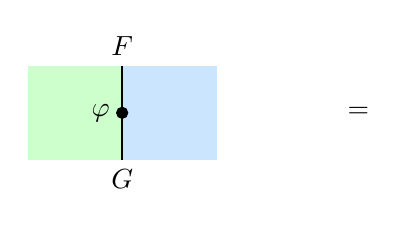
\begin{tikzpicture}[x=0.6cm,y=0.6cm, baseline=(current bounding box.center)]
        % Define colors
        \definecolor{rightcolor}{RGB}{204, 229, 255}
        \definecolor{leftcolor}{RGB}{204,255,204}
    
        % Draw background
        \fill[leftcolor] (0,0) rectangle (2,2);
        \fill[rightcolor] (2,0) rectangle (4,2);
    
        % Draw vertical line and point
        \draw[line width=0.7pt] (2,0) -- (2,2);
        \filldraw [black] (2,1) circle (2pt) node[left=1pt] {$\varphi$};
    
        % Label axes
        \draw (2,0) node[below] {$G$};
        \draw (2,2) node[above] {$F$};
        \draw (7,1) node {$=$};
    \end{tikzpicture}
    \hspace{1cm}
    \begin{tikzcd}[ampersand replacement=\&]
        \mathsf{C} \arrow[r, "F"{name=A, above}, bend left=40] \arrow[r, "G"'{name=B, below}, bend right=40] \&[+30pt] \mathsf{D}
        \arrow[Rightarrow, shorten <=5.5pt, shorten >=5.5pt, from=A.south-|B, to=B, "\varphi"]
    \end{tikzcd}
\end{center}

When we say two string diagrams are equal, we mean that the vertical compositions of natural transformations they represent are equal.

The point(0-cells), strings(1-cells), and 2-cells in a string diagram can be interpreted as follows
\begin{itemize}
    \item 2-cells: categories. 2-cells with different colors represent different categories.
    \item 1-cells: functors. Each 1-cell has exactly two adjacent 2-cells. The left and right adjacent 2-cells are the domain and codomain of the functor respectively. We can think each 1-cell has two end points connected to either a natural transformation or the point at infinity $\infty$. If an end point is connected to $\infty$, then we say that it is a \textbf{free end}. The end point on the top of a string and the end point on the bottom of a string are called the \textbf{top end} and \textbf{bottom end} respectively.
    \item 0-cells: natural transformations. Each 0-cell has exactly two adjacent 1-cells. The top and bottom adjacent 1-cells are the domain and codomain of the natural transformation respectively. 
\end{itemize}

\subsection{Basic Operations}
\subsubsection{Composition of Functors}
If two string $F:\mathsf{C}\to\mathsf{D}$ and $G:\mathsf{D}\to\mathsf{F}$ has the same top ends and bottom ends, then we can glue them together to form a new string $G\circ F$. Depending on whether the top ends and bottom ends are free or not, we can illustrate the following cases


\begin{center}
    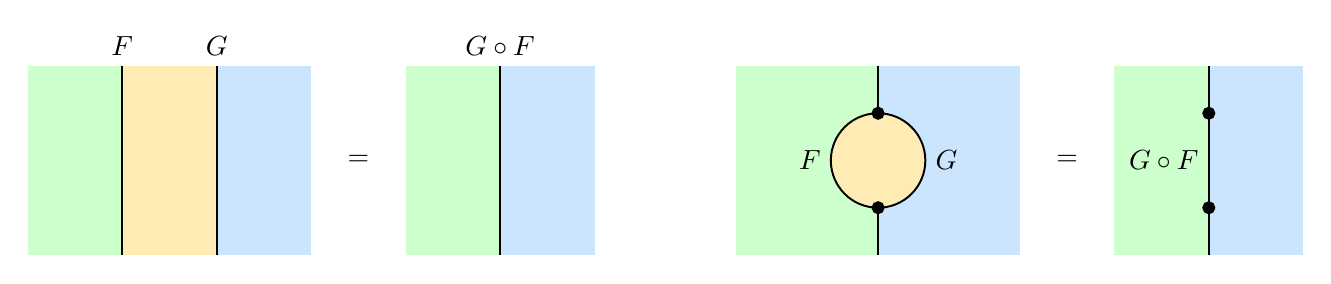
\begin{tikzpicture}[x=0.6cm,y=0.6cm, line width=0.7pt]
            % Define colors
        \definecolor{leftcolor}{RGB}{204,255,204}
        \definecolor{midcolor}{HTML}{FFEBB4} 
        \definecolor{rightcolor}{RGB}{204, 229, 255}
        \begin{scope}
                % Draw background
            \fill[leftcolor] (0,0) rectangle (2,4);
            \fill[midcolor] (2,0) rectangle (4,4);
            \fill[rightcolor] (4,0) rectangle (6,4);
        
            % Draw vertical line and point
            \draw[line width=0.7pt] (2,0) -- (2,4);
            \draw[line width=0.7pt] (4,0) -- (4,4);
    
        
            % Label axes
            \draw (2,4) node[above] {$F$};
            \draw (4,4) node[above] {$G$};
        \end{scope}

        \draw (7,2) node {$=$};

        \begin{scope}[shift={(8,0)}]
            % Draw background
            % Draw background
            \fill[leftcolor] (0,0) rectangle (2,4);
            \fill[rightcolor] (2,0) rectangle (4,4);
        
            % Draw vertical line and point
            \draw[line width=0.7pt] (2,0) -- (2,4);

        
            % Label axes
            \draw (2,4) node[above] {$G\circ F$};
        \end{scope}

        

        \begin{scope}[shift={(16,0)}]
            % Draw background
    
            \fill[leftcolor] (-1,0) rectangle (2,4);
            \fill[rightcolor] (2,0) rectangle (5,4);
            \draw[fill=midcolor, rounded corners=0.6cm, line width=0.7pt] (1,1) rectangle (3, 3);
    
            % Draw vertical line and point
            \draw[line width=0.7pt] (2,0) -- (2,1);
            \draw[line width=0.7pt] (2,3) -- (2,4);
            \filldraw [black] (2,1) circle (2pt);
            \filldraw [black] (2,3) circle (2pt);
        
            % Label axes
            \draw (1,2) node[left] {$F$};
            \draw (3,2) node[right] {$G$};
        \end{scope}
        \draw (22,2) node {$=$};
        \begin{scope}[shift={(23,0)}]
                % Draw background
            % Draw background
            \fill[leftcolor] (0,0) rectangle (2,4);
            \fill[rightcolor] (2,0) rectangle (4,4);
        
            % Draw vertical line and point
            \draw[line width=0.7pt] (2,0) -- (2,4);
            \filldraw [black] (2,1) circle (2pt);
            \filldraw [black] (2,3) circle (2pt);
        
            % Label axes
            \draw (2,2) node[left] {$G\circ F$};
        \end{scope}
    \end{tikzpicture}
\end{center}
\begin{center}
    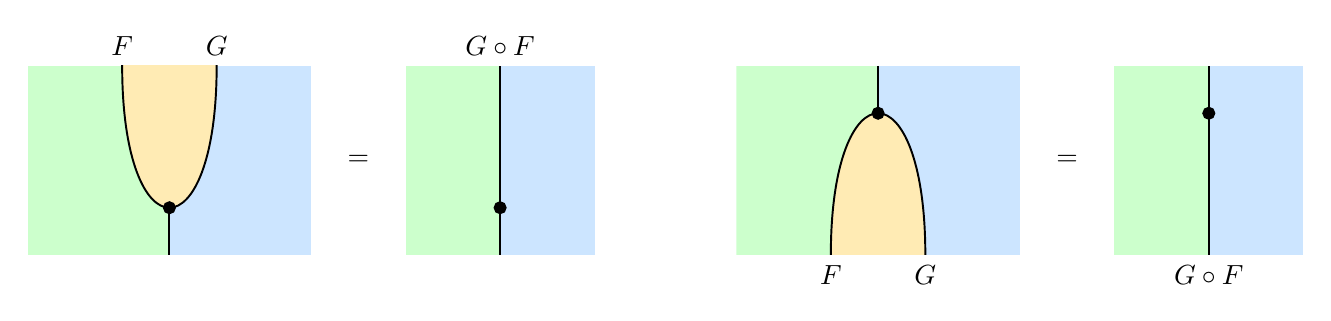
\begin{tikzpicture}[x=0.6cm,y=0.6cm, line width=0.7pt]
        \definecolor{leftcolor}{RGB}{204, 255, 204}
        \definecolor{midcolor}{HTML}{FFEBB4} 
        \definecolor{rightcolor}{RGB}{204, 229, 255}

        \begin{scope}[shift={(0,0)}]
            \begin{scope}
                \clip  (0,0) rectangle (6,4);
                    % Draw background
                \fill[leftcolor] (0,0) rectangle (3,4);
                \fill[rightcolor] (3,0) rectangle (6,4);
                \filldraw[fill=midcolor] (2,5)-- (2,4) .. controls (2,2) and (2.5, 1) .. (3,1).. controls (3.5,1) and (4, 2) .. (4,4)--(4,5)--cycle;
            \end{scope}
        
            % Draw vertical line and point
            \draw[line width=0.7pt] (3,0) -- (3,1);
            \filldraw [black] (3,1) circle (2pt);
            
        
            % Label axes
            \draw (2,4) node[above] {$F$};
            \draw (4,4) node[above] {$G$};
        \end{scope}

        \draw (7,2) node {$=$};

        \begin{scope}[shift={(8,0)}]
            % Draw background
            \fill[leftcolor] (0,0) rectangle (2,4);
            \fill[rightcolor] (2,0) rectangle (4,4);
        
            % Draw vertical line and point
            \draw[line width=0.7pt] (2,0) -- (2,4);
            \filldraw [black] (2,1) circle (2pt);
        
            % Label axes
            \draw (2,4) node[above] {$G\circ F$};
        \end{scope}

            \begin{scope}[shift={(15,0)}]
            \begin{scope}
                \clip  (0,0) rectangle (6,4);
                    % Draw background
                \fill[leftcolor] (0,0) rectangle (3,4);
                \fill[rightcolor] (3,0) rectangle (6,4);
                \filldraw[fill=midcolor] (2,-1)-- (2,0) .. controls (2,2) and (2.5, 3) .. (3,3).. controls (3.5,3) and (4, 2) .. (4,0)--(4,-1)--cycle;
            \end{scope}
        
            % Draw vertical line and point
            \draw[line width=0.7pt] (3,4) -- (3,3);
            \filldraw [black] (3,3) circle (2pt);
            
        
            % Label axes
            \draw (2,0) node[below] {$F$};
            \draw (4,0) node[below] {$G$};
        \end{scope}

        \draw (22,2) node {$=$};

        \begin{scope}[shift={(23,0)}]
            % Draw background
            \fill[leftcolor] (0,0) rectangle (2,4);
            \fill[rightcolor] (2,0) rectangle (4,4);
        
            % Draw vertical line and point
            \draw[line width=0.7pt] (2,0) -- (2,4);
            \filldraw [black] (2,3) circle (2pt);
        
            % Label axes
            \draw (2,0) node[below] {$G\circ F$};
        \end{scope}
    \end{tikzpicture}
\end{center}

\subsubsection{Vertical Composition}
The vertical composition of natural transformations $\varphi:F\Rightarrow H$ and $\psi:G\Rightarrow I$ collapses two adjacent points in a string into one single point and ``eats" the intermediate segment, which is illustrated as follows

\begin{center}
    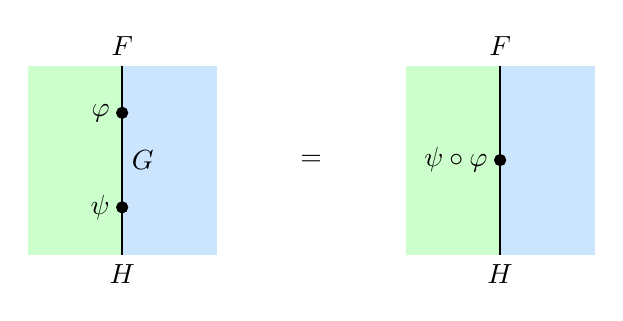
\begin{tikzpicture}[x=0.6cm,y=0.6cm, baseline=(current bounding box.center)]
        % Define colors
        \definecolor{leftcolor}{RGB}{204,255,204}
        \definecolor{rightcolor}{RGB}{204, 229, 255}
        \begin{scope}
            % Draw background
            \fill[leftcolor] (0,-2) rectangle (2,2);
            \fill[rightcolor] (2,-2) rectangle (4,2);
        
        
            % Draw vertical line and point
            \draw[line width=0.7pt] (2,-2) -- (2,2);
            \filldraw [black] (2,1) circle (2pt) node[left=1pt] {$\varphi$};
            \filldraw [black] (2,-1) circle (2pt) node[left=1pt] {$\psi$};
        
            % Label axes
            \draw (2,-2) node[below] {$H$};
            \draw (2,0) node[right] {$G$};
            \draw (2,2) node[above] {$F$};
        \end{scope}

        \draw (6,0) node {$=$};

        \begin{scope}[shift={(8,0)}]
            % Draw background
            \fill[leftcolor] (0,-2) rectangle (2,2);
            \fill[rightcolor] (2,-2) rectangle (4,2);
        
        
            % Draw vertical line and point
            \draw[line width=0.7pt] (2,-2) -- (2,2);
            \filldraw [black] (2,0) circle (2pt) node[left=1pt] {$\psi\circ \varphi$};
    
            % Label axes
            \draw (2,-2) node[below] {$H$};
            \draw (2,2) node[above] {$F$};
        \end{scope}
    \end{tikzpicture}
\end{center}
\subsubsection{Horizontal Composition}
To do horizontal composition for natural transformations $\varphi:F\Rightarrow H$ and $\theta:G\Rightarrow I$ on a horizontal line. First we can stick these two points together, which is illustrated as follows

\begin{center}
    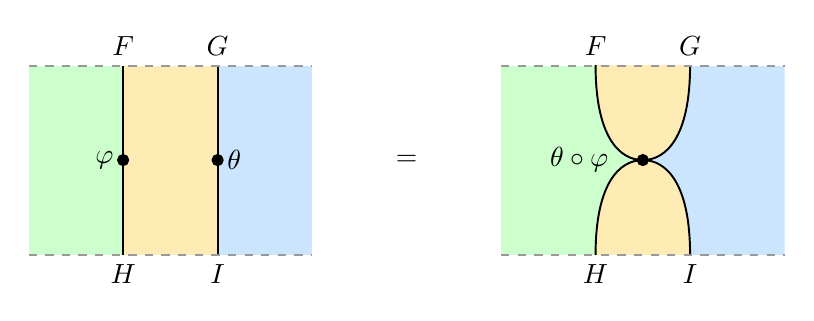
\begin{tikzpicture}[x=0.6cm,y=0.6cm, baseline=(current bounding box.center)]
        \definecolor{leftcolor}{RGB}{204, 255, 204}
        \definecolor{midcolor}{HTML}{FFEBB4} 
        \definecolor{rightcolor}{RGB}{204, 229, 255}

        \begin{scope}
             % Draw background
            \fill[leftcolor] (0,0) rectangle (2,4);
            \fill[midcolor] (2,0) rectangle (4,4);
            \fill[rightcolor] (4,0) rectangle (6,4);
        
            % Draw vertical line and point
            \draw[line width=0.7pt] (2,0) -- (2,4);
            \filldraw [black] (2,2) circle (2pt) node[anchor=east] {$\varphi$};
            \draw[line width=0.7pt] (4,0) -- (4,4);
            \filldraw [black] (4,2) circle (2pt) node[anchor=west] {$\theta$};

            % Draw dashed line
            \draw[dashed, color=black!40, line width=0.7pt] (0,0) -- (6,0);
            \draw[dashed, color=black!40, line width=0.7pt] (0,4) -- (6,4);
        
            % Label axes
            \draw (2,0) node[below] {$H$};
            \draw (2,4) node[above] {$F$};
            \draw (4,0) node[below] {$I$};
            \draw (4,4) node[above] {$G$};
        \end{scope}

        \draw (8,2) node {$=$};

        \begin{scope}[shift={(10,0)}]
             \begin{scope}
                \clip (0,0) rectangle (6,4);
                % Draw background
                \fill[leftcolor] (0,0) rectangle (3,4);
                \fill[rightcolor] (3,0) rectangle (6,4);
                \filldraw[fill=midcolor, line width=0.7pt] (2,5)-- (2,4) .. controls (2, 2.5) and (2.5, 2) .. (3,2).. controls (3.5,2) and (4, 2.5) .. (4,4)--(4,5)--cycle;
                \filldraw[fill=midcolor, line width=0.7pt] (2,-1)-- (2,0) .. controls (2,1.5) and (2.5, 2) .. (3,2).. controls (3.5,2) and (4, 1.5) .. (4,0)--(4,-1)--cycle;
            \end{scope}
        
            % Draw vertical line and point
            \filldraw [black] (3,2) circle (2pt) node[left=9pt] {$\theta\circ\varphi$};

            % Draw dashed line
            \draw[dashed, color=black!40, line width=0.7pt] (0,0) -- (6,0);
            \draw[dashed, color=black!40, line width=0.7pt] (0,4) -- (6,4);

            % Label axes
            \draw (2,0) node[below] {$H$};
            \draw (2,4) node[above] {$F$};
            \draw (4,0) node[below] {$I$};
            \draw (4,4) node[above] {$G$};
        \end{scope}
    \end{tikzpicture}
\end{center}

Then we can composite the functors $F$ and $G$ to get a new functor $G\circ F$. Also we can composite the functors $H$ and $I$ to get a new functor $I\circ H$. By gluing these strings together, we get a new natural transformation $\theta\circ\varphi:G\circ F\Rightarrow I\circ H$. This is illustrated as follows


\begin{center}
    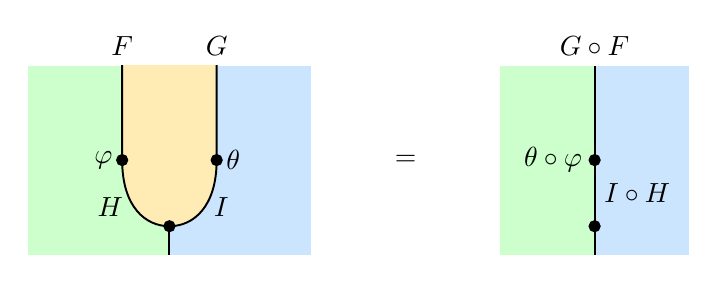
\begin{tikzpicture}[x=0.6cm,y=0.6cm]
        \definecolor{leftcolor}{RGB}{204, 255, 204}
        \definecolor{midcolor}{HTML}{FFEBB4} 
        \definecolor{rightcolor}{RGB}{204, 229, 255}

        \begin{scope}[shift={(0,0)}]
            \begin{scope}
                \clip  (0,0) rectangle (6,4);
                 % Draw background
                \fill[leftcolor] (0,0) rectangle (3,4);
                \fill[rightcolor] (3,0) rectangle (6,4);
                \filldraw[fill=midcolor, line width=0.7pt] (2,5)-- (2,2) .. controls (2,1) and (2.5, 0.6) .. (3,0.6).. controls (3.5,0.6) and (4, 1) .. (4,2)--(4,5)--cycle;
            \end{scope}
        
            % Draw vertical line and point
            \draw[line width=0.7pt] (3,0) -- (3,0.6);
            \filldraw [black] (3,0.6) circle (2pt);
            \filldraw [black] (2,2) circle (2pt) node[anchor=east] {$\varphi$};
            \filldraw [black] (4,2) circle (2pt) node[anchor=west] {$\theta$};

            % Label axes
            \draw (2,4) node[above] {$F$};
            \draw (4,4) node[above] {$G$};
            \draw (1.75,1) node {$H$};
            \draw (4.1,1) node {$I$};
        \end{scope}

        \draw (8,2) node {$=$};

        \begin{scope}[shift={(10,0)}]
            % Draw background
            \fill[leftcolor] (0,0) rectangle (2,4);
            \fill[rightcolor] (2,0) rectangle (4,4);
        
            % Draw vertical line and point
            \draw[line width=0.7pt] (2,0) -- (2,4);
            \filldraw [black] (2,0.6) circle (2pt);
            \filldraw [black] (2,2) circle (2pt) node[left=1pt] {$\theta\circ \varphi$};
            \draw (2, 1.3) node[anchor=west] {$I\circ H$};

            % Label axes
            \draw (2,4) node[above] {$G\circ F$};
        \end{scope}

    \end{tikzpicture}
\end{center}

\subsection{Morphism as Natural Transformation}
If $f:X\to Y$ is a morphism in $\mathsf{C}$, then the following string diagram should be understood as follows
\begin{center}
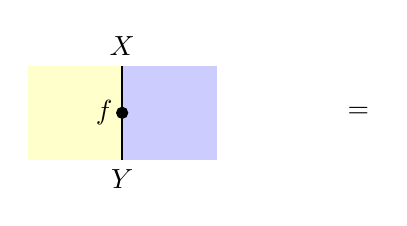
\begin{tikzpicture}[x=0.6cm,y=0.6cm, baseline=(current bounding box.center)]
    % Define colors
    \definecolor{leftcolor}{RGB}{255,255,204} % light yellow
    \definecolor{rightcolor}{RGB}{204,204,255} % light purple

    % Draw background
    \fill[leftcolor] (0,0) rectangle (2,2);
    \fill[rightcolor] (2,0) rectangle (4,2);

    % Draw vertical line and point
    \draw[line width=0.7pt] (2,0) -- (2,2);
    \filldraw [black] (2,1) circle (2pt) node[anchor=east] {$f$};

    % Label axes
    \draw (2,0) node[below] {$Y$};
    \draw (2,2) node[above] {$X$};
    \draw (7,1) node {$=$};
\end{tikzpicture}
\hspace{1cm}
\begin{tikzcd}[ampersand replacement=\&]
    \boldone \arrow[r, "\diagfunctor X"{name=A, above}, bend left=40] \arrow[r, "\diagfunctor Y"'{name=B, below}, bend right=40] \&[+30pt] \mathsf{C}
    \arrow[Rightarrow, shorten <=5.5pt, shorten >=5.5pt, from=A.south-|B, to=B, "f_{\bullet}"]
\end{tikzcd}
\end{center}
\subsubsection{Naturality}
Suppose $\varphi:F\Rightarrow G$ is a natural transformation between functors $F,G:\mathsf{C}\to \mathsf{D}$. Then the functoriality of $\varphi$ can be described by the following string diagram
\[
    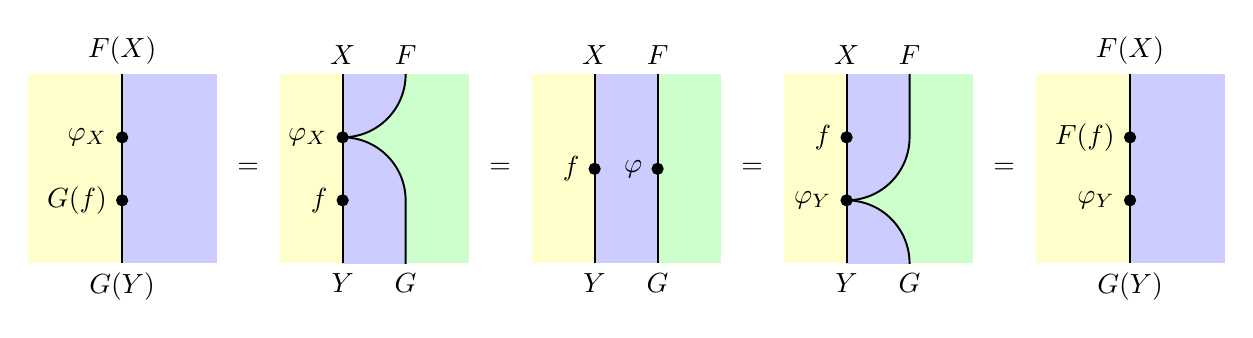
\begin{tikzpicture}[x=0.8cm,y=0.8cm, baseline=(current bounding box.center)]
        % Define colors
        \definecolor{leftcolor}{RGB}{255,255,204} % light yellow
        \definecolor{rightcolor}{RGB}{204,204,255} % light purple
        \begin{scope} [shift={(-3.5,0)}]
        % Draw background
        \fill[leftcolor] (-0.5,0) rectangle (1,3);
        \fill[rightcolor] (1,0) rectangle (2.5,3);
    
        % Draw vertical line and point
        \draw[line width=0.7pt] (1,0) -- (1,3);
        \filldraw [black] (1,1) circle (2pt) node[left=2pt] {$G(f)$};
        \filldraw [black] (1,2) circle (2pt) node[left=2pt] {$\varphi_X$};
        % Label axes
        \draw (1,0) node[below] {$G(Y)$};
        \draw (1,3) node[above] {$F(X)$};
        \draw (3,1.5) node {$=$};
    \end{scope} 
    \begin{scope} 
        % Draw background
        \fill[leftcolor] (0,0) rectangle (1,3);
        \fill[green!20] (1,0) rectangle (3,3);
        \begin{scope} 
            \clip (1,0) rectangle (3, 3); 
            \draw[fill=blue!20, rounded corners=0.8cm, line width=0.7pt] (0,2) rectangle (2, 5);
            \draw[fill=blue!20, rounded corners=0.8cm, line width=0.7pt] (0,2) rectangle (2, -1);
        \end{scope} 
    
        % Draw vertical line and point
        \draw[line width=0.7pt] (1,0) -- (1,3);
        \filldraw [black] (1,1) circle (2pt) node[left=2pt] {$f$};
        \filldraw [black] (1,2) circle (2pt) node[left=2pt] {$\varphi_X$};
        % Label axes
        \draw (1,0) node[below] {$Y$};
        \draw (1,3) node[above] {$X$};
        \draw (2,0) node[below] {$G$};
        \draw (2,3) node[above] {$F$};
        \draw (3.5,1.5) node {$=$};
    \end{scope} 
        
    \begin{scope} [shift={(4,0)}]
        % Define colors
        \definecolor{leftcolor}{RGB}{255,255,204} % light yellow
        \definecolor{rightcolor}{RGB}{204,204,255} % light purple
    
        % Draw background
        \fill[leftcolor] (0,0) rectangle (1,3);
        \fill[blue!20] (1,0) rectangle (2,3);
        \fill[green!20] (2,0) rectangle (3,3);
     
        % Draw vertical line and point
        \draw[line width=0.7pt] (1,0) -- (1,3);
        \draw[line width=0.7pt] (2,0) -- (2,3);
        \filldraw [black] (1,1.5) circle (2pt) node[left=2pt] {$f$};
        \filldraw [black] (2,1.5) circle (2pt) node[left=2pt] {$\varphi$};
        % Label axes
        \draw (1,0) node[below] {$Y$};
        \draw (1,3) node[above] {$X$};
        \draw (2,0) node[below] {$G$};
        \draw (2,3) node[above] {$F$};
        \draw (3.5,1.5) node {$=$};
    \end{scope} 
    
    \begin{scope}[shift={(8,0)}]
        % Define colors
        \definecolor{leftcolor}{RGB}{255,255,204} % light yellow
        \definecolor{rightcolor}{RGB}{204,204,255} % light purple
    
        % Draw background
        \fill[leftcolor] (0,0) rectangle (1,3);
        \fill[green!20] (1,0) rectangle (3,3);
        \begin{scope} 
            \clip (1,0) rectangle (3, 3); 
            \draw[fill=blue!20, rounded corners=0.8cm, line width=0.7pt] (0,1) rectangle (2, 4);
            \draw[fill=blue!20, rounded corners=0.8cm, line width=0.7pt] (0,1) rectangle (2, -2);
            %\fill[color=green!20] (2,0) rectangle (3,3);
            %\filldraw[fill=green!20, rounded corners=1cm] (2, 4) -- (2, 1) -- (1, 1) -- (2, 1) -- (2, -1) -- (4, -1) -- (4, 4) -- cycle;
        \end{scope} 
        % Draw vertical line and point
        \draw[line width=0.7pt] (1,0) -- (1,3);
        \filldraw [black] (1,1) circle (2pt) node[left=2pt] {$\varphi_Y$};
        \filldraw [black] (1,2) circle (2pt) node[left=2pt] {$f$};
        % Label axes
        \draw (1,0) node[below] {$Y$};
        \draw (1,3) node[above] {$X$};
        \draw (2,0) node[below] {$G$};
        \draw (2,3) node[above] {$F$};
        \draw (3.5,1.5) node {$=$};
    \end{scope} 
    
    \begin{scope} [shift={(12.5,0)}]
        % Draw background
        \fill[leftcolor] (-0.5,0) rectangle (1,3);
        \fill[rightcolor] (1,0) rectangle (2.5,3);
    
        % Draw vertical line and point
        \draw[line width=0.7pt] (1,0) -- (1,3);
        \filldraw [black] (1,2) circle (2pt) node[left=2pt] {$F(f)$};
        \filldraw [black] (1,1) circle (2pt) node[left=2pt] {$\varphi_Y$};
        % Label axes
        \draw (1,0) node[below] {$G(Y)$};
        \draw (1,3) node[above] {$F(X)$};
    \end{scope} 
    \end{tikzpicture}
    \]

Note that appending the string diagram 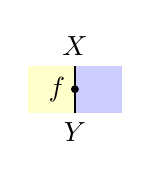
\begin{tikzpicture}[x=0.3cm,y=0.3cm, baseline=(current bounding box.center)]
    % Define colors
    \definecolor{leftcolor}{RGB}{255,255,204} % light yellow
    \definecolor{rightcolor}{RGB}{204,204,255} % light purple

    % Draw background
    \fill[leftcolor] (0,0) rectangle (2,2);
    \fill[rightcolor] (2,0) rectangle (4,2);

    % Draw vertical line and point
    \draw[line width=0.7pt] (2,0) -- (2,2);
    \filldraw [black] (2,1) circle (1.2pt) node[anchor=east] {$f$};

    % Label axes
    \draw (2,0) node[below] {$Y$};
    \draw (2,2) node[above] {$X$};
\end{tikzpicture} to the left of the string diagram of $\varphi$ is equivalent to evaluating $\varphi$ at $f:X\to Y$.

\subsubsection{Elements of Sets}
Let $X$ be a set and $x\in X$ be an element of $X$. Then we represents $x$ as a morphism $x:\{*\}\to X$ in $\mathsf{Set}$, which is illustrated as follows
\begin{center}
    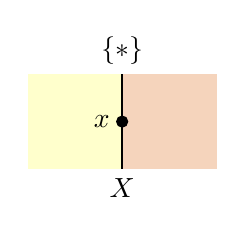
\begin{tikzpicture}[x=0.6cm,y=0.6cm, baseline=(current bounding box.center)]
        % Define colors
        \definecolor{leftcolor}{RGB}{255,255,204} % light yellow
        \definecolor{rightcolor}{HTML}{F5D4BC} % red
    
        % Draw background
        \fill[leftcolor] (0,0) rectangle (2,2);
        \fill[rightcolor] (2,0) rectangle (4,2);
    
        % Draw vertical line and point
        \draw[line width=0.7pt] (2,0) -- (2,2);
        \filldraw [black] (2,1) circle (2pt) node[left=1pt] {$x$};
    
        % Label axes
        \draw (2,0) node[below] {$X$};
        \draw (2,2) node[above] {$\{*\}$};
    \end{tikzpicture}
\end{center}
\subsubsection{Function as Element or Morphism}
If we have a function $f:X\to Y$, then we can represent $f$ as morphism $f:X\to Y$ in $\mathsf{Set}$, which is illustrated as follows
\[
    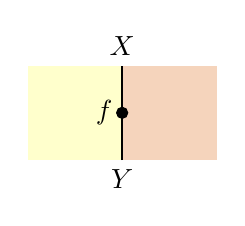
\begin{tikzpicture}[x=0.6cm,y=0.6cm, baseline=(current bounding box.center)]
        % Define colors
        \definecolor{leftcolor}{RGB}{255,255,204} % light yellow
        \definecolor{rightcolor}{HTML}{F5D4BC}  % red
    
        % Draw background
        \fill[leftcolor] (0,0) rectangle (2,2);
        \fill[rightcolor] (2,0) rectangle (4,2);
    
        % Draw vertical line and point
        \draw[line width=0.7pt] (2,0) -- (2,2);
        \filldraw [black] (2,1) circle (2pt) node[anchor=east] {$f$};
    
        % Label axes
        \draw (2,0) node[below] {$Y$};
        \draw (2,2) node[above] {$X$};
    \end{tikzpicture}
\]
And we can also represent $f$ as an element $f\in \mathrm{Hom}_{\mathsf{Set}}(X,Y)$, which is illustrated as follows
\[
    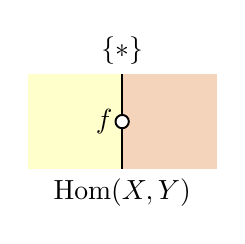
\begin{tikzpicture}[
        x=0.6cm,
        y=0.6cm,
        mydot/.style={
            circle,
            fill=white,
            draw,
            outer sep=0pt,
            inner sep=1.7pt,
            line width=0.7pt
          }]
        % Define colors
        \definecolor{leftcolor}{RGB}{255,255,204} % light yellow
        \definecolor{rightcolor}{HTML}{F5D4BC}  % red
    
        % Draw background
        \fill[leftcolor] (0,0) rectangle (2,2);
        \fill[rightcolor] (2,0) rectangle (4,2);
    
        % Draw vertical line and point
        \draw[line width=0.7pt] (2,0) -- (2,2);
        \draw (2,1) node[mydot] {};
        \draw (2,1) node[left] {$f$};
    
        % Label axes
        \draw (2,0) node[below] {$\mathrm{Hom}(X,Y)$};
        \draw (2,2) node[above] {$\{*\}$};
    \end{tikzpicture}
\]
Then we have the following equalities for Hom functor $\llbracket X , -\rrbracket:\mathsf{C}\to \mathsf{Set}$
\[
 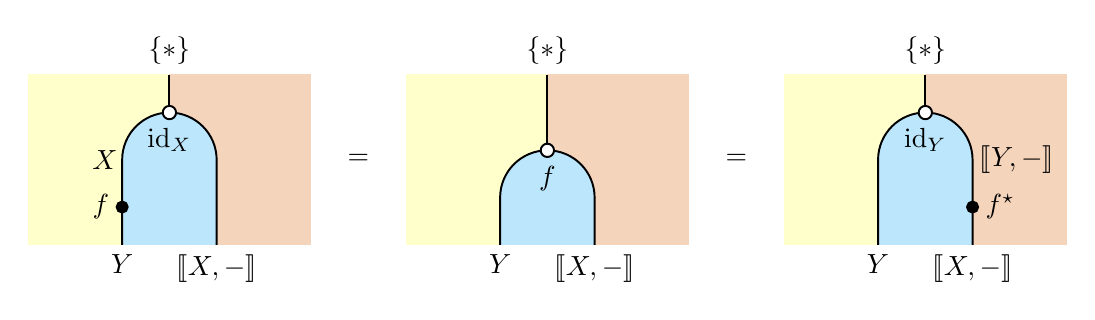
\begin{tikzpicture}[x=0.6cm,y=0.6cm,line width=0.7pt,hollow/.style={
            circle,
            fill=white,
            draw,
            outer sep=0pt,
            inner sep=1.7pt,
            line width=0.7pt
          }]
    \definecolor{leftcolor}{RGB}{255,255,204}
    \definecolor{midcolor}{HTML}{BBE6FB}
    \definecolor{rightcolor}{HTML}{F5D4BC}

    \node at (4, 1.8) {$=$};
    \node at (12, 1.8) {$=$};
    
    \begin{scope}
        \begin{scope} 
            \clip (-3,0) rectangle (3,3.6);     
            \fill[fill=leftcolor] (-3,0) rectangle (0, 4);  
            \fill[fill=rightcolor] (0,0) rectangle (3, 4);  
            \draw[fill=midcolor, rounded corners=0.6cm, line width=0.7pt] (-1, -2) rectangle (1, 2.8);
        \end{scope}
        \draw (0, 3.6) -- (0,2.8);
        \filldraw [black] (-1,0.8) circle (2pt) node[left=1pt] {$f$};
        \node[below] at (-1, 0) {$Y$};
        \node[left=-2pt] at (-1, 1.8) {$X$};
        \node[below] at (1, 0) {$\llbracket X , -\rrbracket$};
        \node[hollow] at (0, 2.8) {};
        \node[below=2pt] at (0, 2.8) {$\mathrm{id}_X$}; 
        \node[above] at (0, 3.6) {$\{*\}$};
    \end{scope}
    
    \begin{scope}[shift={(8,0)}]
        \begin{scope} 
            \clip (-3,0) rectangle (3,3.6);     
            \fill[fill=leftcolor] (-3,0) rectangle (0, 4);  
            \fill[fill=rightcolor] (0,0) rectangle (3, 4);  
            \draw[fill=midcolor, rounded corners=0.6cm, line width=0.7pt] (-1, -2) rectangle (1, 2);
        \end{scope}
        \draw (0, 3.6) -- (0,2);
        \node[below] at (-1, 0) {$Y$};
        \node[below] at (1, 0) {$\llbracket X , -\rrbracket$};
        \node[hollow] at (0, 2) {};
        \node[below=2pt] at (0, 2) {$f$}; 
        \node[above] at (0, 3.6) {$\{*\}$};
    \end{scope}
    
     \begin{scope}[shift={(16,0)}]
        \begin{scope} 
            \clip (-3,0) rectangle (3, 3.6);     
            \fill[fill=leftcolor] (-3,0) rectangle (0, 4);  
            \fill[fill=rightcolor] (0,0) rectangle (3, 4);  
            \draw[fill=midcolor, rounded corners=0.6cm, line width=0.7pt] (-1, -2) rectangle (1, 2.8);
        \end{scope}
        \draw (0, 3.6) -- (0,2.8);
        \filldraw [black] (1,0.8) circle (2pt) node[right=1pt] {$f^\star$};
        \node[below] at (-1, 0) {$Y$};
        \node[right=-1pt] at (1, 1.8) {$\llbracket Y , -\rrbracket$};
        \node[below] at (1, 0) {$\llbracket X , -\rrbracket$};
        \node[hollow] at (0, 2.8) {};
        \node[below=2pt] at (0, 2.8) {$\mathrm{id}_Y$}; 
        \node[above] at (0, 3.6) {$\{*\}$};
    \end{scope}
    
    \end{tikzpicture}
\]
Generally, given $X\xrightarrow{f}Y_1\xrightarrow{g}Y_2$ in $\mathsf{Set}$, we have the following equalities
\[
 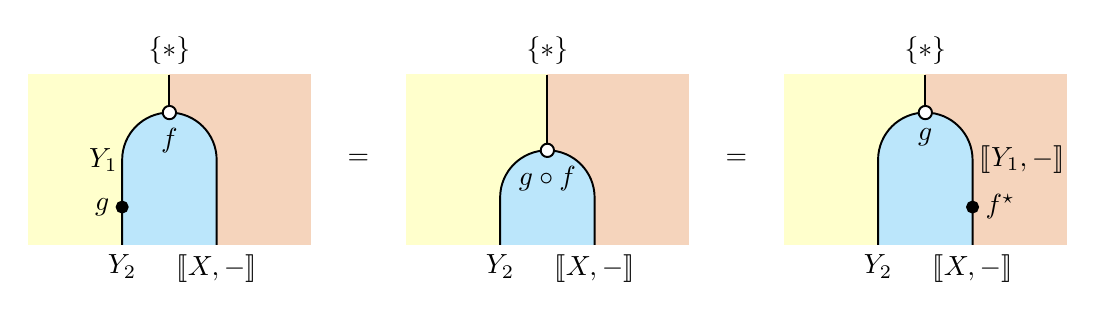
\begin{tikzpicture}[x=0.6cm,y=0.6cm,line width=0.7pt,hollow/.style={
            circle,
            fill=white,
            draw,
            outer sep=0pt,
            inner sep=1.7pt,
            line width=0.7pt
          }]
    \definecolor{leftcolor}{RGB}{255,255,204}
    \definecolor{midcolor}{HTML}{BBE6FB}
    \definecolor{rightcolor}{HTML}{F5D4BC}

    \node at (4, 1.8) {$=$};
    \node at (12, 1.8) {$=$};
    
    \begin{scope}
        \begin{scope} 
            \clip (-3,0) rectangle (3,3.6);     
            \fill[fill=leftcolor] (-3,0) rectangle (0, 4);  
            \fill[fill=rightcolor] (0,0) rectangle (3, 4);  
            \draw[fill=midcolor, rounded corners=0.6cm, line width=0.7pt] (-1, -2) rectangle (1, 2.8);
        \end{scope}
        \draw (0, 3.6) -- (0,2.8);
        \filldraw [black] (-1,0.8) circle (2pt) node[left=1pt] {$g$};
        \node[below] at (-1, 0) {$Y_2$};
        \node[left=-2pt] at (-1, 1.8) {$Y_1$};
        \node[below] at (1, 0) {$\llbracket X , -\rrbracket$};
        \node[hollow] at (0, 2.8) {};
        \node[below=2pt] at (0, 2.8) {$f$}; 
        \node[above] at (0, 3.6) {$\{*\}$};
    \end{scope}
    
    \begin{scope}[shift={(8,0)}]
        \begin{scope} 
            \clip (-3,0) rectangle (3,3.6);     
            \fill[fill=leftcolor] (-3,0) rectangle (0, 4);  
            \fill[fill=rightcolor] (0,0) rectangle (3, 4);  
            \draw[fill=midcolor, rounded corners=0.6cm, line width=0.7pt] (-1, -2) rectangle (1, 2);
        \end{scope}
        \draw (0, 3.6) -- (0,2);
        \node[below] at (-1, 0) {$Y_2$};
        \node[below] at (1, 0) {$\llbracket X , -\rrbracket$};
        \node[hollow] at (0, 2) {};
        \node[below=2pt] at (0, 2) {$g\circ f$}; 
        \node[above] at (0, 3.6) {$\{*\}$};
    \end{scope}
    
     \begin{scope}[shift={(16,0)}]
        \begin{scope} 
            \clip (-3,0) rectangle (3, 3.6);     
            \fill[fill=leftcolor] (-3,0) rectangle (0, 4);  
            \fill[fill=rightcolor] (0,0) rectangle (3, 4);  
            \draw[fill=midcolor, rounded corners=0.6cm, line width=0.7pt] (-1, -2) rectangle (1, 2.8);
        \end{scope}
        \draw (0, 3.6) -- (0,2.8);
        \filldraw [black] (1,0.8) circle (2pt) node[right=1pt] {$f^\star$};
        \node[below] at (-1, 0) {$Y_2$};
        \node[right=-1pt] at (1, 1.8) {$\llbracket Y_1 , -\rrbracket$};
        \node[below] at (1, 0) {$\llbracket X , -\rrbracket$};
        \node[hollow] at (0, 2.8) {};
        \node[below=2pt] at (0, 2.8) {$g$}; 
        \node[above] at (0, 3.6) {$\{*\}$};
    \end{scope}
    
    \end{tikzpicture}
\]
\section{Representable Functor}
\begin{definition}{Presheaf}{}
    Let $\mathsf{C}$ be a category. A \textbf{presheaf} on $\mathsf{C}$ is a functor $F:\mathsf{C}^{\mathrm{op}}\to \mathsf{Set}$.
\end{definition}


\begin{definition}{Yoneda Embedding Functor}{yoneda_embedding_functor}
    Let $\mathsf{C}$ be a category. The \textbf{Yoneda embedding functor} is the functor $Y_\mathsf{C}:\mathsf{C}\to \left[\mathsf{C}^{\mathrm{op}},\mathsf{Set}\right]$ defined as follows
    \[
    \begin{tikzcd}[ampersand replacement=\&]
    \mathsf{C} % column 1
    \&[-25pt]  % column 2
    \&[+30pt]  % column 3
    \&[-30pt] \left[\mathsf{C}^{\mathrm{op}},\mathsf{Set}\right]    % column 4
    \&[+25pt]  % column 5
    \&[-25pt]  % column 6 
    \&         % column 7
    \\[-15pt]
    Y_1 \arrow[dd, "g"{name=L, left}] \&\&  \& \mathrm{Hom}_{\mathsf{C}}\left(-,Y_1\right) \arrow[dd, Rightarrow, "g_\star"{name=R}] \& \mathrm{Hom}_{\mathsf{C}}(X_1,Y_1) \arrow[dd, "{g_*}"'] \arrow[rr, "{f^*}"] \& \& \mathrm{Hom}_{\mathsf{C}}(X_2,Y_1) \arrow[dd, "g_*"] \\[-5pt]
    \& \phantom{.}\arrow[r, "Y_\mathsf{C}", squigarrow]\&\phantom{.} \&\phantom{.} \&\phantom{.}\&\\[-5pt]
    Y_2 \& \& \& \mathrm{Hom}_{\mathsf{C}}\left(-,Y_2\right)\& \mathrm{Hom}_{\mathsf{C}}(X_1,Y_2) \arrow[rr, "{f^*}"'] \& \& \mathrm{Hom}_{\mathsf{C}}(X_2,Y_2) 
    \arrow[from=4-5, to=2-5, dash, start anchor={[xshift=-8ex,yshift=-3ex]}, end anchor={[xshift=-8ex,yshift=3ex]},decorate,decoration={brace,amplitude=10pt,raise=4pt}] 
    \arrow[from=3-4, to=3-5, dashed, start anchor={[xshift=9pt, yshift=-2pt]}, end anchor={[xshift=-11ex, yshift=-2pt]},decorate] 
    \end{tikzcd}
    \]
    where the natural transformation $g_\star$ is defined pointwise as follows: $\left(g_\star\right)_X=g_*$ for any $X\in \mathrm{Ob}(\mathsf{C}^{\mathrm{op}})$.\\
    The contravariant version is $Y_{\mathsf{C}^{\mathrm{op}}}:\mathsf{C}^{\mathrm{op}}\to \left[\mathsf{C},\mathsf{Set}\right]$, which is defined as follows
    \[
    \begin{tikzcd}[ampersand replacement=\&]
    \mathsf{C}^{\mathrm{op}} % column 1
    \&[-25pt]  % column 2
    \&[+30pt]  % column 3
    \&[-30pt] \left[\mathsf{C},\mathsf{Set}\right]    % column 4
    \&[+25pt]  % column 5
    \&[-25pt]  % column 6 
    \&         % column 7
    \\[-15pt]
    X_1 \arrow[dd, "f"{name=L, left}] \&\&  \& \mathrm{Hom}_{\mathsf{C}}\left(X_1,-\right) \arrow[dd, Rightarrow, "f^\star"{name=R}] \& \mathrm{Hom}_{\mathsf{C}}(X_1,Y_1) \arrow[dd, "{f^*}"'] \arrow[rr, "{g_*}"] \& \& \mathrm{Hom}_{\mathsf{C}}(X_1,Y_2) \arrow[dd, "f^*"] \\[-5pt]
    \& \phantom{.}\arrow[r, "Y_{\mathsf{C}^{\mathrm{op}}}", squigarrow]\&\phantom{.} \&\phantom{.} \&\phantom{.}\&\\[-5pt]
    X_2 \& \& \& \mathrm{Hom}_{\mathsf{C}}\left(X_2,-\right)\& \mathrm{Hom}_{\mathsf{C}}(X_2,Y_1) \arrow[rr, "{g_*}"'] \& \& \mathrm{Hom}_{\mathsf{C}}(X_2,Y_2) 
    \arrow[from=4-5, to=2-5, dash, start anchor={[xshift=-8ex,yshift=-3ex]}, end anchor={[xshift=-8ex,yshift=3ex]},decorate,decoration={brace,amplitude=10pt,raise=4pt}] 
    \arrow[from=3-4, to=3-5, dashed, start anchor={[xshift=9pt, yshift=-2pt]}, end anchor={[xshift=-11ex, yshift=-2pt]},decorate] 
    \end{tikzcd}
    \]
    Here we use the fact $\mathrm{Hom}_{\mathsf{C}^{\mathrm{op}}}\left(-,X\right)=\mathrm{Hom}_{\mathsf{C}}\left(X,-\right)$.
    
\end{definition}

\begin{theorem}{Yoneda Lemma}{yoneda_lemma}
    Let $\mathsf{C}$ be a locally small category. For any functor $F:\mathsf{C}^{\mathrm{op}}\to \mathsf{Set}$ and any $A\in \mathrm{Ob}(\mathsf{C})$, there is a natural bijection
    \begin{align*}
        q_{A,F}:\operatorname{Hom}_{\mathsf{Psh}(\mathsf{C})}\left(\operatorname{Hom}_{\mathsf{C}}\left(-,A\right), F\right) & \overset{\sim}{\longrightarrow} F(A) \\
        {  \left[ \begin{tikzcd}[ampersand replacement=\&]
            \mathsf{C}^{\mathrm{op}} \arrow[r, "\operatorname{Hom}_{\mathsf{C}}\left(-{,}A\right)"{name=A, above}, bend left] \arrow[r, "F"'{name=B, below}, bend right] \&[+30pt] \mathsf{Set}
            \arrow[Rightarrow, shorten <=5.5pt, shorten >=5.5pt, from=A.south-|B, to=B, "\phi"]
        \end{tikzcd}\right] } & \longmapsto \phi_A\left(\operatorname{id}_A\right)
    \end{align*}
    The naturality of $q_{A,F}$ means that 
    \[
        \begin{tikzcd}[ampersand replacement=\&]
            \mathsf{C}^{\mathrm{op}}\times \left[\mathsf{C}^{\mathrm{op}},\mathsf{Set}\right]\&[-34pt]\&[+62pt]\&[-25pt] \mathsf{Set}\&[-25pt]\&[-25pt] \\ [-15pt] 
            (A_1,F_1)  \arrow[dd, "\left(g{,} \eta\right)"{name=L, left}] 
            \&[-25pt] \& [+10pt] 
            \& [-30pt]\operatorname{Hom}_{\mathsf{Psh}(\mathsf{C})}(\mathrm{Hom}_{\mathsf{C}}(-,A_1),F_1)\arrow[dd, ""{name=R}] \& \ni \& \phi \arrow[dd,mapsto]\\ [-8pt] 
            \&  \phantom{.}\arrow[r, "\operatorname{Hom}_{\mathsf{Psh}(\mathsf{C})}\left(Y_\mathsf{C}(-){,}-\right)", squigarrow]\&\phantom{.}  \&   \\[-8pt] 
            (A_2,F_2)  \& \& \& \operatorname{Hom}_{\mathsf{Psh}(\mathsf{C})}(\mathrm{Hom}_{\mathsf{C}}(-,A_2),F_2)\& \ni \& \eta\circ \phi\circ g_\star
        \end{tikzcd}
    \]
    is a functor isomorphic to the \hyperref[th:evaluation_functor]{evaluation functor}
    \begin{align*}
        \mathrm{ev}:\mathsf{C}^{\mathrm{op}}\times \left[\mathsf{C}^{\mathrm{op}},\mathsf{Set}\right]&\longrightarrow \mathsf{Set}\\
        \left(A,F\right)&\longmapsto F(A)
    \end{align*}
    \textbf{Covariant version}\\
    For any functor $F:\mathsf{C}\to \mathsf{Set}$ and any $A\in \mathrm{Ob}(\mathsf{C})$, there is a natural bijection
    \begin{align*}
        \operatorname{Hom}_{\left[\mathsf{C},\mathsf{Set}\right]}\left(\operatorname{Hom}_{\mathsf{C}}\left(A,-\right), F\right) & \overset{\sim}{\longrightarrow} F(A) \\
        {  \left[ \begin{tikzcd}[ampersand replacement=\&]
            \mathsf{C} \arrow[r, "\operatorname{Hom}_{\mathsf{C}}\left(A{,}-\right)"{name=A, above}, bend left] \arrow[r, "F"'{name=B, below}, bend right] \&[+30pt] \mathsf{Set}
            \arrow[Rightarrow, shorten <=5.5pt, shorten >=5.5pt, from=A.south-|B, to=B, "\phi"]
        \end{tikzcd}\right] } & \longmapsto \phi_A\left(\operatorname{id}_A\right)
    \end{align*}
\end{theorem}

\begin{prf}
    We break the proof into following steps.
\begin{itemize}[leftmargin=*]
    \item \textbf{$\phi$ is determined by $\phi_A\left(\operatorname{id}_A\right)$}.\\
    Suppose $\phi:\mathrm{Hom}_{\mathsf{C}}\left(-,A\right)\Rightarrow F$ is a natural transformation. Given any morphism $f:X\to A$ in $\mathsf{C}$, the naturality of $\phi$ gives the following commutative diagram
    \[
		\begin{tikzcd}[ampersand replacement=\&, row sep = 3.5em]
			\mathrm{id}_A\arrow[d, mapsto]\&[-25pt]\in\&[-25pt]\mathrm{Hom}_{\mathsf{C}}(A,A) \arrow[d, "{\phi_A}"']  \arrow[rr, "{f^*}"] \&[-20pt] \& {\mathrm{Hom}_{\mathsf{C}}(X,A)} \arrow[d, "\phi_X"]\&[-25pt]\ni\&[-25pt]f \arrow[d, mapsto]\\
			\phi_A(\mathrm{id}_A)\&\in\&{F(A)}\arrow[rr, "{F(f)}"'] \&  \& {F(X)}  \&\ni\& \phi_X(f)     
		\end{tikzcd}
	\]
    Thus we see $\phi$ is determined by $\phi_A(\mathrm{id}_A)$ as follows
    \[
        \phi_X(f)=F(f)(\phi_A(\mathrm{id}_A)),\quad\forall X\in \mathrm{Ob}(\mathsf{C}),\forall f\in \mathrm{Hom}_{\mathsf{C}}(X,A).
    \]
    This implies that the injectivity of $q_{A,F}$.
    \item \textbf{Construct the inverse of $q_{A,F}$}.\\
    Define 
    \begin{align*}
        r_{A,F}:  F(A)&\longrightarrow\operatorname{Hom}_{\mathsf{Psh}(\mathsf{C})}\left(\operatorname{Hom}_{\mathsf{C}}\left(-,A\right), F\right) \\
         u & \longmapsto \phi^u:\left[\begin{aligned}\phi_X^u: \mathrm{Hom}_{\mathsf{C}}(X,A)&\longrightarrow F(X)\\
             f&\longmapsto F(f)(u)\end{aligned}  \right]
    \end{align*}
    To ensure $r_{A,F}$ is well-defined, we need to check that $r_{A,F}(u)=\phi^u$ is always a natural transformation. In fact, given any morphism $h:X_1\to X_2$ in $\mathsf{C}$, it is easy to check the following diagram commutes
    \[
        \begin{tikzcd}[ampersand replacement=\&, row sep = 3.5em]
                g\arrow[mapsto]{d}\&[-25pt]\in\&[-25pt]\mathrm{Hom}_{\mathsf{C}}(X_2,A) \arrow[d, "{\phi_{X_2}^u}"']  \arrow[rr, "{h^*}"] \&[-20pt] \& {\mathrm{Hom}_{\mathsf{C}}(X_1,A)} \arrow[d, "\phi_{X_1}^u"]\&[-25pt]\ni\&[-25pt]g\circ h \arrow[mapsto]{d}\\
                F(g)(u)\&\in\&{F(X_2)}\arrow[rr, "{F(h)}"'] \&  \& {F(X_1)}  \&\ni\& F(g\circ h)(u)  
            \end{tikzcd}
    \]
    because the functoriality of $F$ gives the identity $F(g\circ h)=F(h)\circ F(g)$.

    For any $u\in F(A)$, we have
    \begin{align*}
        \left(q_{A,F}\circ r_{A,F}\right)(u)
        &=q_{A,F}(\phi^u)\\
        &=\phi^u_A(\mathrm{id}_A)\\
        &=F(\mathrm{id}_A)(u)\\
        &=\mathrm{id}_{F(A)}(u)\\
        &=u,
    \end{align*}
    which implies that $q_{A,F}$ is surjective. Therefore, $q_{A,F}$ is a bijection and $r_{A,F}$ is the inverse of $q_{A,F}$.

    We can also manually check that $\left(r_{A,F}\circ q_{A,F}\right)(\phi)=\phi$ for any natural transformation $\phi:\mathrm{Hom}_{\mathsf{C}}\left(-,A\right)\Rightarrow F$, by evaluating the natural transformations at $\mathrm{id}_A$,
    \begin{align*}
        \left(\left(r_{A,F}\circ q_{A,F}\right)(\phi)\right)_A(\mathrm{id}_A)&=(r_{A,F}(\phi_A(\mathrm{id}_A)))_A(\mathrm{id}_A)\\
        &=F(\mathrm{id}_A)(\phi_A(\mathrm{id}_A))\\
        &=\mathrm{id}_{F(A)}(\phi_A(\mathrm{id}_A))\\
        &=\phi_A(\mathrm{id}_A).
    \end{align*}
    \item \textbf{$q_{A,F}$ is natural in $A$ and $F$}.\\
    $\operatorname{Hom}_{\mathsf{Psh}(\mathsf{C})}\left(Y_\mathsf{C}(-){,}-\right)$ is a functor obtained by the composition 
    \[
        \mathsf{C}^{\mathrm{op}}\times \left[\mathsf{C}^{\mathrm{op}},\mathsf{Set}\right]\xrightarrow{\left(Y^{\mathrm{op}}_{\mathsf{C}},\mathrm{id}\right)}\left[\mathsf{C}^{\mathrm{op}},\mathsf{Set}\right]^{\mathrm{op}}\times \left[\mathsf{C}^{\mathrm{op}},\mathsf{Set}\right]\xrightarrow{\mathrm{Hom}_{\mathsf{Psh}(\mathsf{C})}\left(-,-\right)}\mathsf{Set}
    \]
    Given any $g:A_2\to A_1$ and $\eta:F_1\to F_2$, we should check the following diagram commutes
    \[
        \begin{tikzcd}[row sep=3.5em, column sep=2.5em, ampersand replacement=\&]
        {\operatorname{Hom}_{\mathsf{Psh}(\mathsf{C})}(Y_\mathsf{C}(A_1),F_1)} \arrow[d, "{q_{A_1,F_1}}"'] \arrow[rr, "\left(g_\star\right)^*\circ \eta_*"] \&  \& {\operatorname{Hom}_{\mathsf{Psh}(\mathsf{C})}(Y_\mathsf{C}(A_2),F_2)} \arrow[d, "q_{A_2,F_2}"] \\
        {F_1(A_1)} \arrow[rr, "F_2(g)\circ \eta_{A_1}"']      \&  \& {F_2(A_2)}               
    \end{tikzcd}
    \]
    It suffices to check that the following diagram commutes
    \[
    \begin{tikzcd}[ampersand replacement=\&, row sep = 3.5em]
        \operatorname{Hom}(Y_\mathsf{C}(A_1),F_1) \arrow[rr,"\left(g_\star\right)^*"] \arrow[dr,swap,"\eta_*"] \arrow[dd,swap,"q_{A_1,F_1}"] \&\&
        \operatorname{Hom}(Y_\mathsf{C}(A_2),F_1) \arrow[dd,swap,"q_{A_2,F_1}" near start] \arrow[dr,"\eta_*"] \\
        \& \operatorname{Hom}(Y_\mathsf{C}(A_1),F_2) \arrow[rr,crossing over,"\left(g_\star\right)^*" near start] \&\&
        \operatorname{Hom}(Y_\mathsf{C}(A_2),F_2) \arrow[dd,"q_{A_2,F_2}"] \\
        F_1(A_1) \arrow[rr,"F_1(g)" near end] \arrow[dr,swap,"\eta_{A_1}"] \&\& F_1(A_2) \arrow[dr,swap,"\eta_{A_2}"] \\
        \& F_2(A_1) \arrow[rr,"F_2(g)"] \arrow[uu,<-,crossing over,"q_{A_1,F_2}" near end]\&\& F_2(A_2)
        \end{tikzcd}
    \]
\end{itemize}
    To check the commutativity of the left square
    \[
        \begin{tikzcd}[row sep=3.5em, column sep=2.5em, ampersand replacement=\&]
        {\operatorname{Hom}_{\mathsf{Psh}(\mathsf{C})}(Y_\mathsf{C}(A_1),F_1)} \arrow[d, "{q_{A_1,F_1}}"'] \arrow[rr, "\eta_*"] \&  \& {\operatorname{Hom}_{\mathsf{Psh}(\mathsf{C})}(Y_\mathsf{C}(A_1),F_2)} \arrow[d, "q_{A_1,F_2}"] \\
        {F_1(A_1)} \arrow[rr, "\eta_{A_1}"']      \&  \& {F_2(A_1)}               
    \end{tikzcd}
    \]
    we can verify that for any $\phi\in \operatorname{Hom}_{\mathsf{Psh}(\mathsf{C})}\left(Y_\mathsf{C}(A_1),F_1\right)$, 
    \begin{align*}
        q_{A_1,F_2}\circ \eta_*\left(\phi\right)&=q_{A_1,F_2}\left(\eta\circ \phi\right)\\
        &=\left(\eta\circ \phi\right)_{A_1}\left(\mathrm{id}_{A_1}\right)\\
        &=\eta_{A_1}(\phi_{A_1}(\mathrm{id}_{A_1}))\\
        &=\eta_{A_1}\circ q_{A_1,F_1}(\phi).
    \end{align*}
    To check the commutativity of the front square
    \[
        \begin{tikzcd}[row sep=3.5em, column sep=2.5em, ampersand replacement=\&]
        {\operatorname{Hom}_{\mathsf{Psh}(\mathsf{C})}(Y_\mathsf{C}(A_1),F_2)} \arrow[d, "{q_{A_1,F_2}}"'] \arrow[rr, "\left(g_\star\right)^*"] \&  \& {\operatorname{Hom}_{\mathsf{Psh}(\mathsf{C})}(Y_\mathsf{C}(A_2),F_2)} \arrow[d, "q_{A_2,F_2}"] \\
        {F_2(A_1)} \arrow[rr, "F_2(g)"']      \&  \& {F_2(A_2)}               
    \end{tikzcd}
    \]
    we can verify that for any $\psi\in \operatorname{Hom}_{\mathsf{Psh}(\mathsf{C})}\left(Y_\mathsf{C}(A_1),F_2\right)$, we have
    \begin{align*}
        q_{A_2,F_2}\circ \left(g_\star\right)^*(\psi)&=q_{A_2,F_2}\left(\psi\circ g_\star\right)\\
        &=\left(\psi\circ g_\star\right)_{A_2}\left(\mathrm{id}_{A_2}\right)\\
        &=\psi_{A_2}\circ g_*\left(\mathrm{id}_{A_2}\right)\\
        &=\psi_{A_2}(g)\\
        &=F_2(g)(\psi_{A_1}(\mathrm{id}_{A_1}))\\
        &=F_2(g)\circ q_{A_1,F_2}(\psi).
    \end{align*}
\end{prf}

\noindent For the covariant version, the following string diagram shows $\phi$ is determined by $\phi_A\left(\operatorname{id}_A\right)$
\[
        \phi_X(f)=F(f)(\phi_A(\mathrm{id}_A)),\quad\forall X\in \mathrm{Ob}(\mathsf{C}),\forall f\in \mathrm{Hom}_{\mathsf{C}}(A,X).
\]
\[
    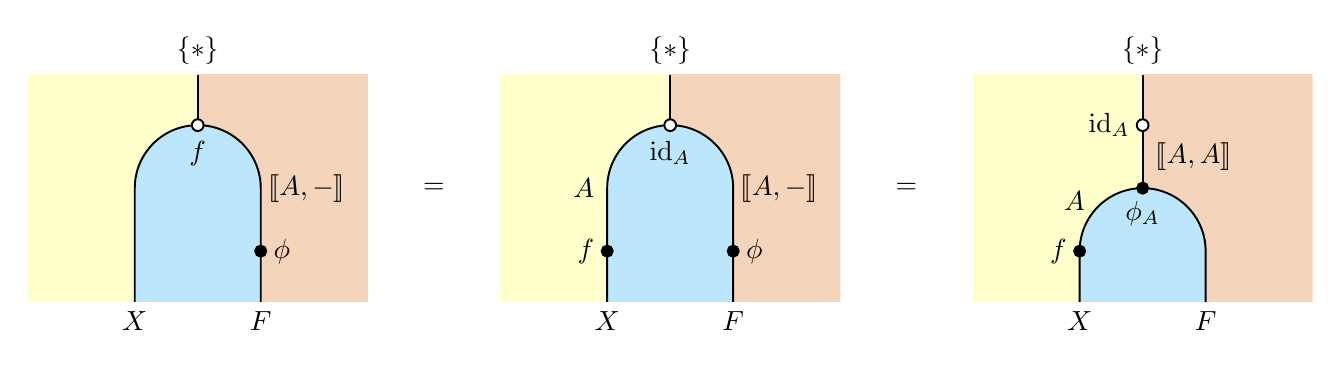
\begin{tikzpicture}[x=0.8cm,y=0.8cm, line width=0.7pt, hollow/.style={
            circle,
            fill=white,
            draw,
            outer sep=0pt,
            inner sep=1.5pt,
            line width=0.7pt
          }]
        % Define colors
         \definecolor{leftcolor}{RGB}{255,255,204}
    \definecolor{midcolor}{HTML}{BBE6FB}
    \definecolor{rightcolor}{HTML}{F5D4BC}

    \node at (-3.75, 1.8) {$=$};
    \node at (3.75, 1.8) {$=$};

    \begin{scope}[shift={(-7.5,0)}]
        \begin{scope} 
            \clip (-2.7,0) rectangle (2.7, 3.6);     
            \fill[fill=leftcolor] (-3,0) rectangle (0, 4);  
            \fill[fill=rightcolor] (0,0) rectangle (3, 4);  
            \draw[fill=midcolor, rounded corners=0.8cm, line width=0.7pt] (-1, -2) rectangle (1, 2.8);
        \end{scope}
        \draw (0, 3.6) -- (0,2.8);
        \filldraw [black] (1,0.8) circle (2pt) node[right=1pt] {$\phi$};
        \node[below] at (-1, 0) {$X$};
        \node[right=-1pt] at (1, 1.8) {$\llbracket A , -\rrbracket$};
        \node[below] at (1, 0) {$F$};
        \node[hollow] at (0, 2.8) {};
        \node[below=2pt] at (0, 2.8) {$f$}; 
        \node[above] at (0, 3.6) {$\{*\}$};
    \end{scope}

    \begin{scope}[shift={(0,0)}]
        \begin{scope} 
            \clip (-2.7,0) rectangle (2.7, 3.6);     
            \fill[fill=leftcolor] (-3,0) rectangle (0, 4);  
            \fill[fill=rightcolor] (0,0) rectangle (3, 4);  
            \draw[fill=midcolor, rounded corners=0.8cm, line width=0.7pt] (-1, -2) rectangle (1, 2.8);
        \end{scope}
        \draw (0, 3.6) -- (0,2.8);
        \filldraw [black] (1,0.8) circle (2pt) node[right=1pt] {$\phi$};
        \filldraw [black] (-1,0.8) circle (2pt) node[left=1pt] {$f$};
        \node[below] at (-1, 0) {$X$};
        \node[right=-1pt] at (1, 1.8) {$\llbracket A , -\rrbracket$};
        \node[left=1pt] at (-1, 1.8) {$A$};
        \node[below] at (1, 0) {$F$};
        \node[hollow] at (0, 2.8) {};
        \node[below=2pt] at (0, 2.8) {$\mathrm{id}_A$}; 
        \node[above] at (0, 3.6) {$\{*\}$};
    \end{scope}

    \begin{scope}[shift={(7.5,0)}]
        \begin{scope} 
            \clip (-2.7,0) rectangle (2.7, 3.6);     
            \fill[fill=leftcolor] (-3,0) rectangle (0, 4);  
            \fill[fill=rightcolor] (0,0) rectangle (3, 4);  
            \draw[fill=midcolor, rounded corners=0.8cm, line width=0.7pt] (-1, -3) rectangle (1, 1.8);
        \end{scope}
        \draw (0, 3.6) -- (0, 1.8);
        \filldraw [black] (-1,0.8) circle (2pt) node[left=1pt] {$f$};
        \filldraw [black] (0,1.8) circle (2pt) node[below=1pt] {$\phi_A$};
        \node[below] at (-1, 0) {$X$};
        \node at (-1.08, 1.6) {$A$};
        \node[below] at (1, 0) {$F$};
        \node[hollow] at (0, 2.8) {};
        \node[right=1pt] at (0, 2.3) {$\llbracket A , A\rrbracket$}; 
        \node[left=1pt] at (0, 2.8) {$\mathrm{id}_A$}; 
        \node[above] at (0, 3.6) {$\{*\}$};
    \end{scope}
    \end{tikzpicture}
\]

\noindent For any $u\in F(A)$, we can define $\phi^u:\mathrm{Hom}_{\mathsf{C}}\left(A,-\right)\Rightarrow F$ by

\[
    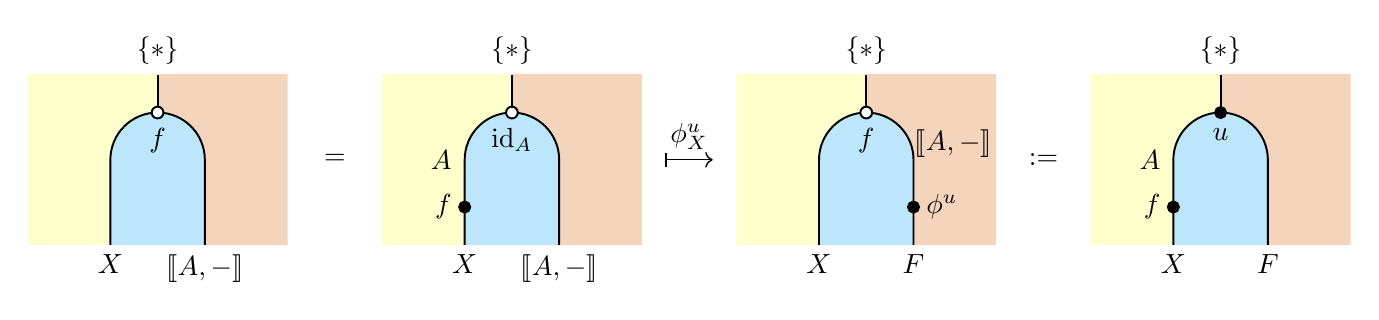
\begin{tikzpicture}[x=0.6cm,y=0.6cm, line width=0.7pt, hollow/.style={
            circle,
            fill=white,
            draw,
            outer sep=0pt,
            inner sep=1.5pt,
            line width=0.7pt
          }]
        % Define colors
    \definecolor{leftcolor}{RGB}{255,255,204}
    \definecolor{midcolor}{HTML}{BBE6FB}
    \definecolor{rightcolor}{HTML}{F5D4BC}

    \node at (-3.75, 1.8) {$=$};
    \draw [|-To, line width=0.5pt] (3.25,1.8) -- (4.25,1.8) node[midway,above] {$\phi^u_X$};
    \node at (11.25, 1.8) {$:=$};

    \begin{scope}[shift={(-7.5,0)}]
        \begin{scope} 
            \clip (-2.75,0) rectangle (2.75, 3.6);     
            \fill[fill=leftcolor] (-3,0) rectangle (0, 4);  
            \fill[fill=rightcolor] (0,0) rectangle (3, 4);  
            \draw[fill=midcolor, rounded corners=0.6cm, line width=0.7pt] (-1, -2) rectangle (1, 2.8);
        \end{scope}
        \draw (0, 3.6) -- (0,2.8);
        \node[below] at (-1, 0) {$X$};
        \node[below] at (1, 0) {$\llbracket A , -\rrbracket$};
        \node[hollow] at (0, 2.8) {};
        \node[below=2pt] at (0, 2.8) {$f$}; 
        \node[above] at (0, 3.6) {$\{*\}$};
    \end{scope}

    \begin{scope}[shift={(0,0)}]
        \begin{scope} 
            \clip (-2.75,0) rectangle (2.75, 3.6);     
            \fill[fill=leftcolor] (-3,0) rectangle (0, 4);  
            \fill[fill=rightcolor] (0,0) rectangle (3, 4);  
            \draw[fill=midcolor, rounded corners=0.6cm, line width=0.7pt] (-1, -2) rectangle (1, 2.8);
        \end{scope}
        \draw (0, 3.6) -- (0,2.8);
        \filldraw [black] (-1,0.8) circle (2pt) node[left=1pt] {$f$};
        \node[below] at (-1, 0) {$X$};
        \node[left=1pt] at (-1, 1.8) {$A$};
        \node[below] at (1, 0) {$\llbracket A , -\rrbracket$};
        \node[hollow] at (0, 2.8) {};
        \node[below=2pt] at (0, 2.8) {$\mathrm{id}_A$}; 
        \node[above] at (0, 3.6) {$\{*\}$};
    \end{scope}

    \begin{scope}[shift={(7.5,0)}]
       \begin{scope} 
            \clip (-2.75,0) rectangle (2.75, 3.6);     
            \fill[fill=leftcolor] (-3,0) rectangle (0, 4);  
            \fill[fill=rightcolor] (0,0) rectangle (3, 4);  
            \draw[fill=midcolor, rounded corners=0.6cm, line width=0.7pt] (-1, -2) rectangle (1, 2.8);
        \end{scope}
        \draw (0, 3.6) -- (0,2.8);
        \filldraw [black] (1,0.8) circle (2pt) node[right=1pt] {$\phi^u$};
        \node[below] at (-1, 0) {$X$};
        \node[right=-1.5pt] at (0.9, 2.15) {$\llbracket A , -\rrbracket$};
        \node[below] at (1, 0) {$F$};
        \node[hollow] at (0, 2.8) {};
        \node[below=2pt] at (0, 2.8) {$f$}; 
        \node[above] at (0, 3.6) {$\{*\}$};
    \end{scope}
    
    \begin{scope}[shift={(15,0)}]
       \begin{scope} 
            \clip (-2.75,0) rectangle (2.75, 3.6);     
            \fill[fill=leftcolor] (-3,0) rectangle (0, 4);  
            \fill[fill=rightcolor] (0,0) rectangle (3, 4);  
            \draw[fill=midcolor, rounded corners=0.6cm, line width=0.7pt] (-1, -2) rectangle (1, 2.8);
        \end{scope}
        \draw (0, 3.6) -- (0,2.8);
        \filldraw [black] (-1,0.8) circle (2pt) node[left=1pt] {$f$};
        \filldraw [black] (0, 2.8) circle (2pt) node[below=2pt] {$u$};
        \node[below] at (-1, 0) {$X$};
        \node[left=1pt] at (-1, 1.8) {$A$};
        \node[below] at (1, 0) {$F$};
        \node[above] at (0, 3.6) {$\{*\}$};
    \end{scope}
    \end{tikzpicture}
\]

\noindent and check that the naturality of $\phi^u$ as follows

\[
    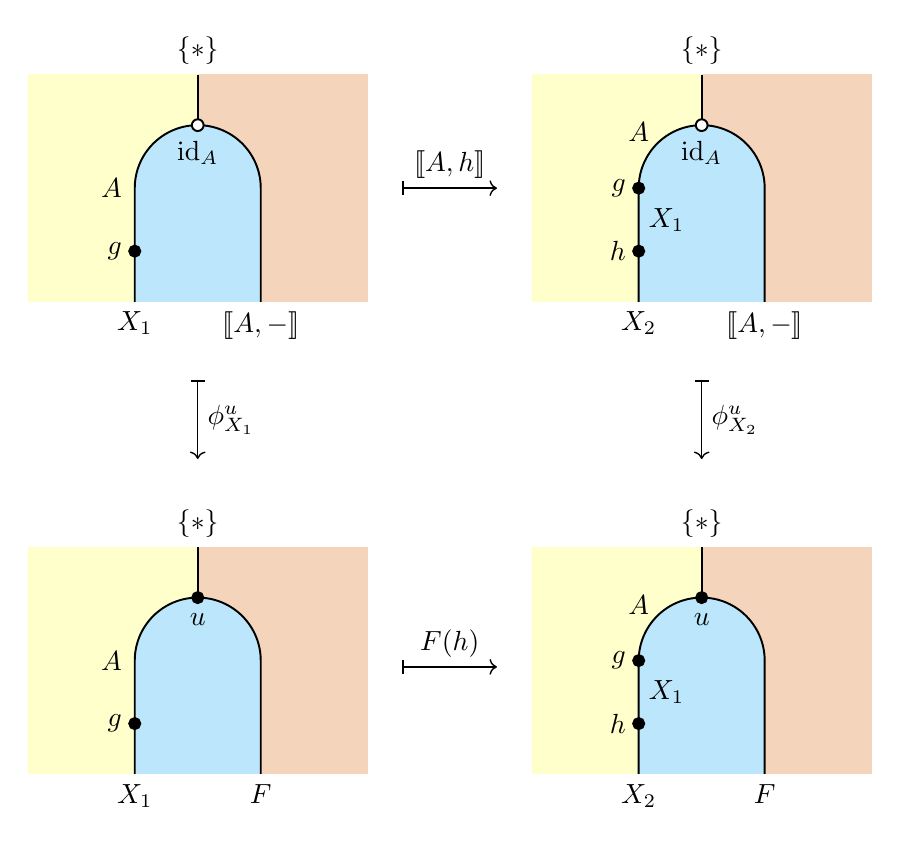
\begin{tikzpicture}[x=0.8cm,y=0.8cm, line width=0.7pt, hollow/.style={
            circle,
            fill=white,
            draw,
            outer sep=0pt,
            inner sep=1.5pt,
            line width=0.7pt
          }]
        % Define colors
         \definecolor{leftcolor}{RGB}{255,255,204}
    \definecolor{midcolor}{HTML}{BBE6FB}
    \definecolor{rightcolor}{HTML}{F5D4BC}

    \draw [|-To, line width=0.5pt] (-4.75,-5.8) -- (-3.25,-5.8) node[midway,above] {$F(h)$};
    \draw [|-To, line width=0.5pt] (0,-1.25) -- (0,-2.5) node[midway,right] {$\phi^u_{X_2}$};
    \draw [|-To, line width=0.5pt] (-4.75,1.8) -- (-3.25,1.8) node[midway,above] {$\llbracket A , h\rrbracket$};
    \draw [|-To, line width=0.5pt] (-8,-1.25) -- (-8,-2.5) node[midway,right] {$\phi^u_{X_1}$};  

    \begin{scope}[shift={(-8,0)}]
        \begin{scope} 
            \clip (-2.7,0) rectangle (2.7, 3.6);     
            \fill[fill=leftcolor] (-3,0) rectangle (0, 4);  
            \fill[fill=rightcolor] (0,0) rectangle (3, 4);  
            \draw[fill=midcolor, rounded corners=0.8cm, line width=0.7pt] (-1, -2) rectangle (1, 2.8);
        \end{scope}
        \draw (0, 3.6) -- (0,2.8);
        \filldraw [black] (-1,0.8) circle (2pt) node[left=1pt] {$g$};
        \node[below] at (-1, 0) {$X_1$};
        \node[left=1pt] at (-1, 1.8) {$A$};
        \node[below] at (1, 0) {$\llbracket A , -\rrbracket$};
        \node[hollow] at (0, 2.8) {};
        \node[below=2pt] at (0, 2.8) {$\mathrm{id}_A$}; 
        \node[above] at (0, 3.6) {$\{*\}$};
    \end{scope}

    \begin{scope}[shift={(-8,-7.5)}]
       \begin{scope} 
            \clip (-2.7,0) rectangle (2.7, 3.6);     
            \fill[fill=leftcolor] (-3,0) rectangle (0, 4);  
            \fill[fill=rightcolor] (0,0) rectangle (3, 4);  
            \draw[fill=midcolor, rounded corners=0.8cm, line width=0.7pt] (-1, -2) rectangle (1, 2.8);
        \end{scope}
        \draw (0, 3.6) -- (0,2.8);
        \filldraw [black] (-1,0.8) circle (2pt) node[left=1pt] {$g$};
        \filldraw [black] (0, 2.8) circle (2pt) node[below=2pt] {$u$};
        \node[below] at (-1, 0) {$X_1$};
        \node[left=1pt] at (-1, 1.8) {$A$};
        \node[below] at (1, 0) {$F$};
        \node[above] at (0, 3.6) {$\{*\}$};
    \end{scope}

    \begin{scope}[shift={(0,-7.5)}]
        \begin{scope} 
            \clip (-2.7,0) rectangle (2.7, 3.6);     
            \fill[fill=leftcolor] (-3,0) rectangle (0, 4);  
            \fill[fill=rightcolor] (0,0) rectangle (3, 4);  
            \draw[fill=midcolor, rounded corners=0.8cm, line width=0.7pt] (-1, -2) rectangle (1, 2.8);
        \end{scope}
        \draw (0, 3.6) -- (0,2.8);
        \node[below] at (-1, 0) {$X_2$};
        \node[right] at (-1, 1.3) {$X_1$};
        \node[below] at (-1, 3) {$A$};
        \node[below] at (1, 0) {$F$};
        % \node[hollow] at (0, 2.8) {};
        % \node[below=2pt] at (0, 2.8) {$u$}; 
        \filldraw [black] (-1,1.8) circle (2pt) node[left=1pt] {$g$};
        \filldraw [black] (-1,0.8) circle (2pt) node[left=1pt] {$h$};
        \filldraw [black] (0, 2.8) circle (2pt) node[below=2pt] {$u$};
        \node[above] at (0, 3.6) {$\{*\}$};
    \end{scope}

     \begin{scope}[shift={(0,0)}]
        \begin{scope} 
            \clip (-2.7,0) rectangle (2.7, 3.6);     
            \fill[fill=leftcolor] (-3,0) rectangle (0, 4);  
            \fill[fill=rightcolor] (0,0) rectangle (3, 4);  
            \draw[fill=midcolor, rounded corners=0.8cm, line width=0.7pt] (-1, -2) rectangle (1, 2.8);
        \end{scope}
        \draw (0, 3.6) -- (0,2.8);
        \node[below] at (-1, 0) {$X_2$};
        \node[right] at (-1, 1.3) {$X_1$};
        \node[below] at (-1, 3) {$A$};
        \node[below] at (1, 0) {$\llbracket A , -\rrbracket$};
        \node[hollow] at (0, 2.8) {};
        \node[below=2pt] at (0, 2.8) {$\mathrm{id}_A$}; 
        \filldraw [black] (-1,1.8) circle (2pt) node[left=1pt] {$g$};
        \filldraw [black] (-1,0.8) circle (2pt) node[left=1pt] {$h$};
        \node[above] at (0, 3.6) {$\{*\}$};
    \end{scope}
    
    \end{tikzpicture}    
\]
Then it is straightforward to see $\phi^u_{A}\left(\mathrm{id_A}\right)=u$ and $\phi^{\phi_A(\mathrm{id}_A)}=\phi$.


\begin{corollary}{Yoneda Embedding}{}
    Let $\mathsf{C}$ be a locally small category. The \hyperref[th:yoneda_embedding_functor]{Yoneda embedding functor} $Y_\mathsf{C}:\mathsf{C}\to \left[\mathsf{C}^{\mathrm{op}},\mathsf{Set}\right]$ is fully faithful. That is, for any $A_1,A_2\in\mathrm{Ob}\left(\mathsf{C}\right)$, the morphism set map 
    \begin{align*}
        \left.Y_{\mathsf{C}}\right|_{\operatorname{Hom}_{\mathsf{C}}\left(A_1,A_2\right)}:\operatorname{Hom}_{\mathsf{C}}\left(A_1,A_2\right) &\longrightarrow\operatorname{Hom}_{\mathsf{Psh}(\mathsf{C})}\left(\operatorname{Hom}_{\mathsf{C}}\left(-,A_1\right), \operatorname{Hom}_{\mathsf{C}}\left(-,A_2\right)\right) \\
         f & \longmapsto f_\star
    \end{align*}
    is a bijection. That justifies the name ``embedding'' because $\mathsf{C}$ is embedded into $\mathsf{Psh}(\mathsf{C})$ via $Y_\mathsf{C}$ as a full subcategory.
\end{corollary}

\begin{prf}
    By \hyperref[th:yoneda_lemma]{Yoneda lemma}, there is a natural bijection
    \[
        \operatorname{Hom}_{\mathsf{Psh}(\mathsf{C})}\left(\operatorname{Hom}_{\mathsf{C}}\left(-,A_1\right), \operatorname{Hom}_{\mathsf{C}}\left(-,A_2\right)\right)\cong \operatorname{Hom}_{\mathsf{C}}\left(A_1,A_2\right),
    \]
    which is given by
    \begin{align*}
        r_{A_1,Y_{\mathsf{C}}(A_2)}:  \operatorname{Hom}_{\mathsf{C}}\left(A_1,A_2\right) &\xlongrightarrow{\sim}\operatorname{Hom}_{\mathsf{Psh}(\mathsf{C})}\left(\operatorname{Hom}_{\mathsf{C}}\left(-,A_1\right), \operatorname{Hom}_{\mathsf{C}}\left(-,A_2\right)\right) \\
         f & \longmapsto f_\star:\left[\begin{aligned}\left(f_\star\right)_X: \mathrm{Hom}_{\mathsf{C}}(X,A_1)&\longrightarrow \mathrm{Hom}_{\mathsf{C}}(X,A_2)\\
             g&\longmapsto f_*(g)=f\circ g\end{aligned}  \right]
    \end{align*}
    and
    \begin{align*}
        q_{A_1,Y_{\mathsf{C}}(A_2)}:\operatorname{Hom}_{\mathsf{Psh}(\mathsf{C})}\left(\operatorname{Hom}_{\mathsf{C}}\left(-,A_1\right), \operatorname{Hom}_{\mathsf{C}}\left(-,A_2\right)\right) & \xlongrightarrow{\sim}\operatorname{Hom}_{\mathsf{C}}\left(A_1,A_2\right) \\
        {  \left[ \begin{tikzcd}[ampersand replacement=\&]
            \mathsf{C}^{\mathrm{op}} \arrow[r, "\operatorname{Hom}_{\mathsf{C}}\left(-{,}A_1\right)"{name=A, above}, bend left] \arrow[r, "\operatorname{Hom}_{\mathsf{C}}\left(-{,}A_2\right)"'{name=B, below}, bend right] \&[+30pt] \mathsf{Set}
            \arrow[Rightarrow, shorten <=5.5pt, shorten >=5.5pt, from=A.south-|B, to=B, "\phi"]
        \end{tikzcd}\right] } & \longmapsto \phi_{A_1}\left(\operatorname{id}_{A_1}\right)
    \end{align*}
    Note that $r_{A_1,Y_{\mathsf{C}}(A_2)}$ is exactly the morphism set map $\left.Y_{\mathsf{C}}\right|_{\operatorname{Hom}_{\mathsf{C}}\left(A_1,A_2\right)}$.
\end{prf}

Yoneda embedding allows us to regard any category $\mathsf{C}$ as a full subcategory of $\mathsf{Psh}(\mathsf{C})$. So in the sense of categorical isomorphism, we can identify any object $A\in \mathrm{Ob}(\mathsf{C})$ with a presheaf $\operatorname{Hom}_{\mathsf{C}}(-, A)$. 

An object in a category is equivalent to the collection of all arrows pointing to that object. In other words, the information we care about is which arrows from an object itself and other objects would point to this object, while the object's internals are completely regarded as a black box. 

The arrows between objects in a category are equivalent to the transformations between sets of arrows pointing to objects. Specifically, suppose $f$ is an arrow from object $A$ to object $B$, then any arrow pointing to $A$ can be transformed into an arrow pointing to $B$ by appending an $f$, which is exactly what $f_\star$ does. Conversely, if there is a way to naturally transform all arrows pointing to $A$ into arrows pointing to $B$, then this transformation must be realized by appending an arrow between $A$ and $B$.

\begin{definition}{Representable Functor}{}
    Let $\mathsf{C}$ be a locally small category. 
    \begin{itemize}
        \item A functor $F:\mathsf{C}\to \mathsf{Set}$ is called \textbf{representable} if it is naturally isomorphic to $\operatorname{Hom}_{\mathsf{C}}\left(A,-\right)$ for some $A\in \mathrm{Ob}(\mathsf{C})$.
        \item A functor $F:\mathsf{C}^{\mathrm{op}}\to \mathsf{Set}$ is called \textbf{representable} if it is naturally isomorphic to $\operatorname{Hom}_{\mathsf{C}}\left(-,A\right)$ for some $A\in \mathrm{Ob}(\mathsf{C})$.
    \end{itemize}
    A \textbf{representation of $F$} is a pair $(A,\phi)$, where $A\in \mathrm{Ob}(\mathsf{C})$ and $\phi:  \operatorname{Hom}_{\mathsf{C}}\left(A,-\right)\xRightarrow{\sim} F$ is a natural isomorphism. \\
    According to \hyperref[th:yoneda_lemma]{Yoneda lemma}, $\phi:\operatorname{Hom}_{\mathsf{C}}\left(A,-\right)\Rightarrow  F$ is 1-1 correspondence with an element $\phi_A(\mathrm{id}_A)\in F(A)$. We define an \textbf{universal element of $F$} is a pair $(A,u)$ where $A\in \mathrm{Ob}(\mathsf{C})$ and $u\in F(A)$ such that $u$ corresponds to a natural isomorphism $\phi: \operatorname{Hom}_{\mathsf{C}}\left(A,-\right)\xRightarrow{\sim} F$. Specifying a universal element of $F$ is equivalent to specifying a representation of $F$.
\end{definition}

\[
 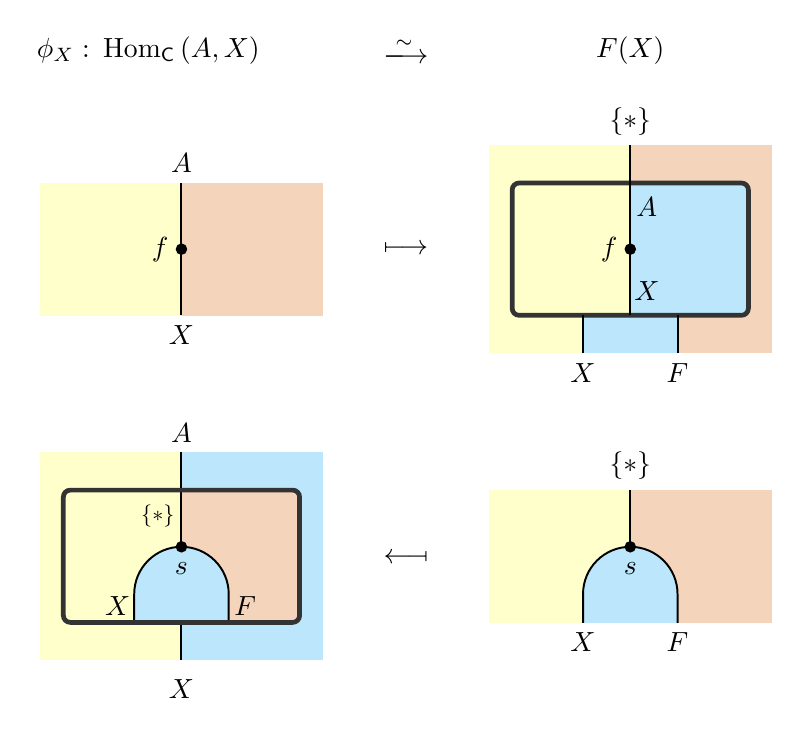
\begin{tikzpicture}[x=0.6cm,y=0.6cm, baseline=(current bounding box.center), line width=0.7pt]
    \definecolor{leftcolor}{RGB}{255,255,204}
    \definecolor{midcolor}{HTML}{BBE6FB}
    \definecolor{rightcolor}{HTML}{F5D4BC}
    \node at (-2.5, 6) {$\phi_{X}:$};
    \node at (0, 6) {$\mathrm{Hom}_{\mathsf{C}}\left(A,X\right)$};
    \node at (4.75, 6) {$\xlongrightarrow{\sim}$};
    \node at (4.75, -4.75) {$\longmapsfrom$};
    \node at (4.75, 1.8) {$\longmapsto$};
    \node at (9.5, 6) {$F(X)$};
    
    \begin{scope}[line width=0.7pt]
        \begin{scope}
            \clip (-3,0.4) rectangle (3,3.2);     
            \fill[fill=leftcolor] (-3,0) rectangle (0, 3.2);  
            \fill[fill=rightcolor] (0,0) rectangle (3, 3.2);  
        \end{scope}
        \node[below] at (0, 0.4) {$X$};
        \node[left=1pt] at (0, 1.8) {$f$};
        \draw[fill=black] (0, 1.8) circle (0.1);  
        \draw (0, 3.2) -- (0, 0.4);
        \node[above] at (0, 3.2) {$A$};
    \end{scope}

    \begin{scope}[shift={(9.5,0)}]
    \fill[fill=leftcolor] (-3,-0.4) rectangle (0,4); 
     \fill[fill=rightcolor] (0, -0.4) rectangle (3,4); 
     \fill[fill=midcolor] (-1, -0.4) rectangle (1,2); 
        \begin{scope} 
            \clip (-2.5,0.4) rectangle (2.5,3.2);     
            \fill[fill=leftcolor] (-2.5,0) rectangle (0, 3.2);  
            \fill[fill=midcolor] (0,0) rectangle (2.5, 3.2);  
        \end{scope}
        \draw[line width=1.7pt, color=black!80, rounded corners=2.5pt] (-2.5, 0.4) rectangle (2.5, 3.2); % inner rectangle
        \node[above,shift={(0.35,0.1)}] at (0, 0.4) {$X$};
        \node[left=1pt] at (0, 1.8) {$f$};
        \draw[fill=black] (0, 1.8) circle (0.1);  
        \draw (0, 4) -- (0, 0.4);
        \node[below,shift={(0.35,-0.1)}] at (0, 3.2) {$A$};
        \draw (1, 0.4) -- (1, -0.4);
        \draw (-1, 0.4) -- (-1, -0.4);
        \node[above] at (0, 4) {$\{*\}$};
        \node[below] at (-1, -0.4) {$X$};
        \node[below] at (1, -0.4) {$F$};
    \end{scope}
    
    \begin{scope}[shift={(0, -6.5)}, line width=0.7pt]
    \fill[fill=leftcolor] (-3,-0.4) rectangle (0,4); 
     \fill[fill=midcolor] (0, -0.4) rectangle (3,4); 
        \begin{scope} 
            \clip (-2.5,0.4) rectangle (2.5, 3.2);     
            \fill[fill=leftcolor] (-2.5,0) rectangle (0, 3.2);  
            \fill[fill=rightcolor] (0,0) rectangle (2.5, 3.2);  
            \draw[fill=midcolor, rounded corners=0.6cm] (-1, -2) rectangle (1, 2);
        \end{scope}
        \node[shift={(-0.35,0.35)}] at (-1, 0.4) {$X$};
        \node[shift={(0.35,0.35)}] at (1, 0.4) {$F$};
        \node[below=2pt] at (0, 2) {$s$};
        \draw[fill=black] (0, 2) circle (0.1);  
        \draw (0,4) -- (0,2);
        \draw (0, -0.4) -- (0,0.4);
        \node[below,shift={(-0.5,0.1)}] at (0, 3) {\scalebox{.8}{$\{*\}$}};
        \draw[line width=1.7pt, color=black!80, rounded corners=2.5pt] (-2.5, 0.4) rectangle (2.5, 3.2); % inner rectangle
        \node[above] at (0, 4){$A$};
        \node[below] at (0, -0.6){$X$};
    \end{scope}

    \begin{scope}[shift={(9.5, -6.5)}, line width=0.7pt]
        \begin{scope} 
            \clip (-3,0.4) rectangle (3,3.2);     
            \fill[fill=leftcolor] (-3,0) rectangle (0, 3.2);  
            \fill[fill=rightcolor] (0,0) rectangle (3, 3.2);  
            \draw[fill=midcolor, rounded corners=0.6cm] (-1, -2) rectangle (1, 2);
        \end{scope}
        \node[below] at (-1, 0.4) {$X$};
        \node[below] at (1, 0.4) {$F$};
        \node[below=2pt] at (0, 2) {$s$};
        \draw[fill=black] (0, 2) circle (0.1);  
        \draw (0,3.2) -- (0,2);
        \node[above] at (0, 3.2) {$\{*\}$};
    \end{scope}
    \end{tikzpicture}
\]

The naturality diagram of $\phi$ 
\[
    \begin{tikzcd}[ampersand replacement=\&, row sep = 3.5em]
        \mathrm{Hom}_{\mathsf{C}}(A,X) \arrow[d, "{\phi_X}"'{name=L, left}, "{\sim}"{name=R, right}]  \arrow[rr, "{h_*}"] \&[-20pt] \& {\mathrm{Hom}_{\mathsf{C}}(A,Y)} \arrow[d, "{\phi_Y}"'{name=L, right}, "{\sim}"{name=R, left}]\\
        {F(X)}\arrow[rr, "{F(h)}"'] \&  \& {F(Y)}  
    \end{tikzcd}
\]
can be translated into the following calculus rules

\[
 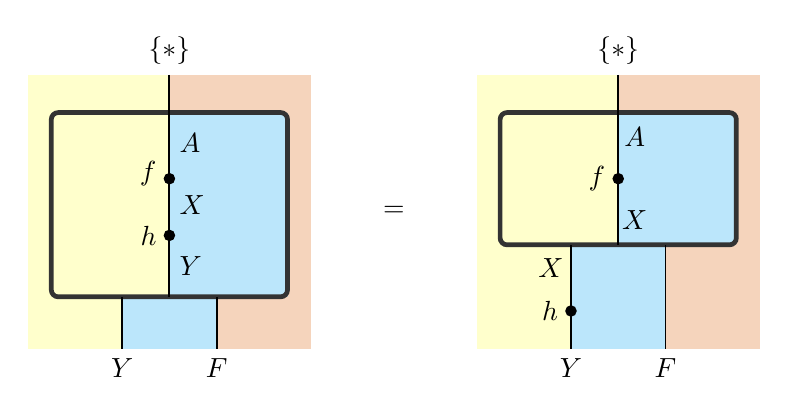
\begin{tikzpicture}[x=0.6cm,y=0.6cm, baseline=(current bounding box.center), line width=0.7pt]
    \definecolor{leftcolor}{RGB}{255,255,204}
    \definecolor{rightcolor}{HTML}{BBE6FB}
    \definecolor{midcolor}{HTML}{F5D4BC}

    \node at (4.75, 1.1) {$=$};
  
    \begin{scope}[shift={(9.5,0)}]
     \fill[fill=leftcolor] (-3,-1.8) rectangle (0,4); 
     \fill[fill=midcolor] (0, -1.8) rectangle (3,4); 
     \fill[fill=rightcolor] (-1, -1.8) rectangle (1,2); 
        \begin{scope} 
            \clip (-2.5,0.4) rectangle (2.5,3.2);     
            \fill[fill=leftcolor] (-2.5,0) rectangle (0, 3.2);  
            \fill[fill=rightcolor] (0,0) rectangle (2.5, 3.2);  
        \end{scope}
        \draw[line width=1.7pt, color=black!80, rounded corners=2.5pt] (-2.5, 0.4) rectangle (2.5, 3.2); % inner rectangle
        \node[above,shift={(0.35,0.1)}] at (0, 0.4) {$X$};
        \node[left=1pt] at (0, 1.8) {$f$};
        \draw[fill=black] (0, 1.8) circle (0.1);  
        \draw (0, 4) -- (0, 0.4);
        \node[below,shift={(0.35,-0.1)}] at (0, 3.2) {$A$};
        \draw (1, 0.4) -- (1, -1.8);
        \draw (-1, 0.4) -- (-1, -1.8);
        \node[above] at (0, 4) {$\{*\}$};
        \node[below] at (-1, -1.8) {$Y$};
        \node[below] at (1, -1.8) {$F$};
        \node[left=-1pt] at (-1, -0.1) {$X$};
        \filldraw [black] (-1, -1) circle (0.1) node[left=1pt] {$h$};
    \end{scope}

    \begin{scope}
    \fill[fill=leftcolor] (-3,-1.8) rectangle (0,4); 
     \fill[fill=midcolor] (0, -1.8) rectangle (3,4); 
     \fill[fill=rightcolor] (-1, -1.8) rectangle (1,2); 
        \begin{scope} 
            \clip (-2.5,-0.7) rectangle (2.5,3.2);     
            \fill[fill=leftcolor] (-2.5,-2) rectangle (0, 3.2);  
            \fill[fill=rightcolor] (0,-2) rectangle (2.5, 3.2);  
        \end{scope}
        \draw[line width=1.7pt, color=black!80, rounded corners=2.5pt] (-2.5, -0.7) rectangle (2.5, 3.2); % inner rectangle
        \node[right] at (0, 1.25) {$X$};
        \node[left=1pt] at (0, 1.9) {$f$};
        \draw[fill=black] (0, 1.8) circle (0.1);  
        \draw (0, 4) -- (0, -0.7);
        \node[right] at (0, 2.55) {$A$};
        \draw (1, -0.7) -- (1, -1.8);
        \draw (-1, -0.7) -- (-1, -1.8);
        \node[above] at (0, 4) {$\{*\}$};
        \node[below] at (-1, -1.8) {$Y$};
        \node[below] at (1, -1.8) {$F$};
        \node[right] at (0, -0.05) {$Y$};
        \filldraw [black] (0, 0.6) circle (0.1) node[left=1pt] {$h$};
    \end{scope}
   
    \end{tikzpicture}
\]
\[
 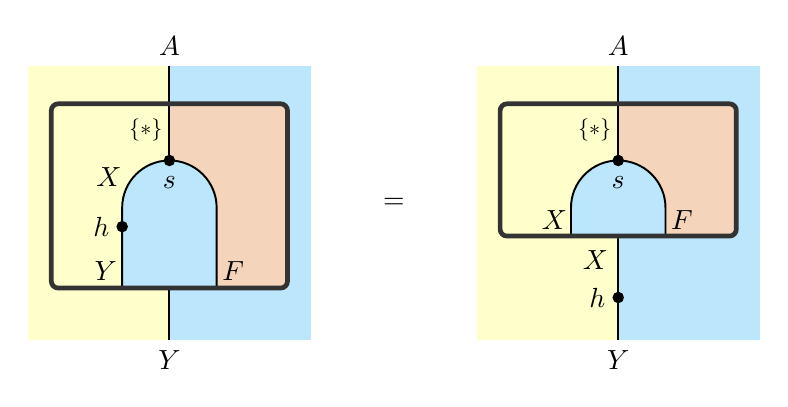
\begin{tikzpicture}[x=0.6cm,y=0.6cm, baseline=(current bounding box.center), line width=0.7pt]
    \definecolor{leftcolor}{RGB}{255,255,204}
    \definecolor{rightcolor}{HTML}{BBE6FB}
    \definecolor{midcolor}{HTML}{F5D4BC}

    \node at (4.75, 1.1) {$=$};
  
    \begin{scope}[shift={(9.5,0)}]
   \fill[fill=leftcolor] (-3,-1.8) rectangle (0,4); 
     \fill[fill=rightcolor] (0, -1.8) rectangle (3,4); 
        \begin{scope} 
            \clip (-2.5,0.4) rectangle (2.5, 3.2);     
            \fill[fill=leftcolor] (-2.5,0) rectangle (0, 3.2);  
            \fill[fill=midcolor] (0,0) rectangle (2.5, 3.2);  
            \draw[fill=rightcolor, rounded corners=0.6cm] (-1, -2) rectangle (1, 2);
        \end{scope}
        \node[shift={(-0.35,0.35)}] at (-1, 0.4) {$X$};
        \node[shift={(0.35,0.35)}] at (1, 0.4) {$F$};
        \node[below=2pt] at (0, 2) {$s$};
        \draw[fill=black] (0, 2) circle (0.1);  
        \draw (0,4) -- (0,2);
        \draw (0, -1.8) -- (0,0.4);
        \node[below,shift={(-0.5,0.1)}] at (0, 3) {\scalebox{.8}{$\{*\}$}};
        \draw[line width=1.7pt, color=black!80, rounded corners=2.5pt] (-2.5, 0.4) rectangle (2.5, 3.2); % inner rectangle
        \node[above] at (0, 4){$A$};
        \node[left] at (0, -0.1){$X$};
        \node[below] at (0, -1.8){$Y$};
        \filldraw [black] (0, -0.9) circle (0.1) node[left=1pt] {$h$};
    \end{scope}

    \begin{scope}
   \fill[fill=leftcolor] (-3,-1.8) rectangle (0,4); 
     \fill[fill=rightcolor] (0, -1.8) rectangle (3,4); 
        \begin{scope} 
            \clip (-2.5,-0.7) rectangle (2.5, 3.2);     
            \fill[fill=leftcolor] (-2.5,0) rectangle (0, 3.2);  
            \fill[fill=midcolor] (0,-1) rectangle (2.5, 3.2);  
            \draw[fill=rightcolor, rounded corners=0.6cm] (-1, -2) rectangle (1, 2);
        \end{scope}
        \node[shift={(-0.35,0.35)}] at (-1, -0.7) {$Y$};
        \node[shift={(0.35,0.35)}] at (1, -0.7) {$F$};
        \node[below=2pt] at (0, 2) {$s$};
        \draw[fill=black] (0, 2) circle (0.1);  
        \draw (0,4) -- (0,2);
        \draw (0, -1.8) -- (0, -0.7);
        \node[below,shift={(-0.5,0.1)}] at (0, 3) {\scalebox{.8}{$\{*\}$}};
        \draw[line width=1.7pt, color=black!80, rounded corners=2.5pt] (-2.5, -0.7) rectangle (2.5, 3.2); % inner rectangle
        \node[above] at (0, 4){$A$};
        \node[left] at (-0.8, 1.65){$X$};
        \node[below] at (0, -1.8){$Y$};
        \filldraw [black] (-1, 0.6) circle (0.1) node[left=1pt] {$h$};
    \end{scope}   
    \end{tikzpicture}
\]


\begin{proposition}{Equivalent Characterizations of Representable Functor}{representable_functor_by_universal_element}
    Suppose $F:\mathsf{C}\to \mathsf{Set}$ is a functor. Then the following statements are equivalent:
    \begin{enumerate}[(i)]
        \item $F$ is representable by universal element $(A,u)$ 
        \item $(A,u)$ is initial in the category \hyperref[th:category_of_elements]{$\int_{\mathsf{C}}F$}$=\left(\{*\} \downarrow F\right)$, which corresponds to $ \begin{tikzcd}[ampersand replacement=\&]
            \boldone \arrow[r, "\diagfunctor\{*\}"] \& \mathsf{Set} \& \mathsf{C}  \arrow[l, " F"']
        \end{tikzcd}$.
        \item $(A,\phi^u)$ is initial in the category $\left(  \text{\hyperref[th:yoneda_embedding_functor]{$Y_{\mathsf{C}^{\mathrm{op}}}$}}\downarrow F\right)$, which corresponds to $ \begin{tikzcd}[ampersand replacement=\&]
           \mathsf{C}^{\mathrm{op}}  \arrow[r, " Y_{\mathsf{C}^{\mathrm{op}}}"] \& \left[\mathsf{C},\mathsf{Set}\right] \&  \boldone \arrow[l, "\diagfunctor F"']
        \end{tikzcd}$.
        \item $\left(A,\diagfunctor u:\{*\}\to F(A)\right)$ is a \hyperref[th:universal_morphism]{universal morphism} from $\{*\}$ to $F$.
        \item For any $(X,x)\in \mathrm{Ob}(\int_{\mathsf{C}}F)$, there is a unique morphism $(A,u)\to (X,x)$ in $\int_{\mathsf{C}}F$ (which is a morphism $f:A\to X$ in $\mathsf{C}$ such that $F(f)(u)=x$).
    \end{enumerate}
    Suppose $F:\mathsf{C}^{\mathrm{op}}\to \mathsf{Set}$ is a functor. Then the following statements are equivalent:
    \begin{enumerate}[(i)]
        \item $F$ is representable by universal element $(A,u)$ 
        \item $(A,u)$ is initial in the category \hyperref[th:category_of_elements]{$\int_{\mathsf{C}^{\mathrm{op}}}F$}$=\left(\{*\} \downarrow F\right)$, which corresponds to $ \begin{tikzcd}[ampersand replacement=\&]
            \boldone \arrow[r, "\diagfunctor\{*\}"] \& \mathsf{Set} \& \mathsf{C}^{\mathrm{op}}  \arrow[l, " F"']
        \end{tikzcd}$.
        \item $(A,\phi^u)$ is terminal in the category $\left(  \text{\hyperref[th:yoneda_embedding_functor]{$Y_{\mathsf{C}}$}}\downarrow F\right)$, which corresponds to $ \begin{tikzcd}[ampersand replacement=\&]
           \mathsf{C} \arrow[r, " Y_{\mathsf{C}}"] \& \left[\mathsf{C}^{\mathrm{op}},\mathsf{Set}\right] \&  \boldone \arrow[l, "\diagfunctor F"']
        \end{tikzcd}$.
        \item $\left(A,\diagfunctor u:\{*\}\to F(A)\right)$ is a \hyperref[th:universal_morphism]{universal morphism} from $\{*\}$ to $F$.
        \item For any $(X,x)\in \mathrm{Ob}\left(\int_{\mathsf{C}^{\mathrm{op}} }F\right)$, there is a unique morphism $(A,u)\to (X,x)$ in $\int_{\mathsf{C}^{\mathrm{op}} }F$ (which is a morphism $f: X\to A$ in $\mathsf{C}$ such that $F(f)(x)=u$).
    \end{enumerate}
\end{proposition}

\begin{prf}
    (i)$\iff$ (ii). Suppose $(A,u)$ is an object of $\int_{\mathsf{C}}F$ and $\phi^u:\operatorname{Hom}_{\mathsf{C}}\left(A,-\right)\Rightarrow F$ be the natural transformation
    \[
        \phi^u_X(f)=F(f)(u),\quad\forall f\in \mathrm{Hom}_{\mathsf{C}}(A,X),
    \]
    which can be illustrated by the following diagram
    \[
		\begin{tikzcd}[ampersand replacement=\&, row sep = 3.5em]
			\mathrm{id}_A\arrow[d, mapsto]\&[-25pt]\in\&[-25pt]\mathrm{Hom}_{\mathsf{C}}(A,A) \arrow[d, "{\phi_A^u}"']  \arrow[rr, "{f_*}"] \&[-20pt] \& {\mathrm{Hom}_{\mathsf{C}}(A,X)} \arrow[d, "\phi_X^u"]\&[-25pt]\ni\&[-25pt]f \arrow[d, mapsto]\\
			u=\phi_A^u(\mathrm{id}_A)\&\in\&{F(A)}\arrow[rr, "{F(f)}"'] \&  \& {F(X)}  \&\ni\& \phi_X^u(f)     
		\end{tikzcd}
	\]   
    Thus we have
    \begin{align*}
        (A,u)\text{ is initial in }\int_{\mathsf{C}}F&\iff \forall(X,x)\in \mathrm{Ob}\left(\int_{\mathsf{C}}F\right),\;\exists! f\in \mathrm{Hom}_{\mathsf{C}}(A,X),\;F(f)(u)=x\\
        &\iff\forall X\in \mathrm{Ob}\left(\mathsf{C}\right),\; \forall x\in F(X),\;\exists! f\in \mathrm{Hom}_{\mathsf{C}}(A,X),\;\phi_X^u(f)=x\\
        &\iff \forall X\in \mathrm{Ob}\left(\mathsf{C}\right),\;\phi_X^u \text{ is bijective}\\
        &\iff \phi^u \text{ is a natural isomorphism}\\
        &\iff (A,u) \text{ is a universal element of }F.
    \end{align*}
    \[
        \begin{tikzcd}[ampersand replacement=\&, row sep=9pt]
              \& F(A) \arrow[dd, dashed, "F(f)"]\\
            \{*\}\arrow[ru, "\diagfunctor u"]\arrow[rd, "\diagfunctor x"']\& \\
             \& F\left(X\right)
            \end{tikzcd}
    \]
    (i)$\iff$ (iii). $\left(A,\phi^u\right)$ is initial in $\left(  Y_{\mathsf{C}^{\mathrm{op}}}\downarrow F\right)$ if and only if for any $ X\in \mathrm{Ob}\left(\mathsf{C}\right)$ and any natural transformation $\psi:\mathrm{Hom}_\mathsf{C}\left(X,-\right)\implies F$, there is a unique $f\in \mathrm{Hom}_{\mathsf{C}}(A,X)$ such that $\phi^u\circ f^\star=\psi$
    \[
        \begin{tikzcd}[ampersand replacement=\&, row sep=9pt]
               \mathrm{Hom}_{\mathsf{C}}\left(A,-\right) \arrow[rd, "\phi^u"]\&\\
            \& F\\
             \mathrm{Hom}_{\mathsf{C}}\left(X,-\right) \arrow[ru, "\psi"']\arrow[uu, dashed, "f^\star"]\& 
            \end{tikzcd}
    \]
    or equivalently
    \[
        \psi_X(\mathrm{id}_X)=\left(\phi^u\circ f^\star\right)_X(\mathrm{id}_X)=\phi^u_X(f).
    \]
    Suppose $F$ is representable by universal element $(A,u)$. Then $\phi^u:\mathrm{Hom}_\mathsf{C}\left(A,-\right)\xRightarrow{\sim} F$ is a natural isomorphism. Since
    \begin{align*}
        \left.Y_{\mathsf{C}^{\mathrm{op}}}\right|_{\operatorname{Hom}_{\mathsf{C}}\left(A,X\right)}:\operatorname{Hom}_{\mathsf{C}}\left(A,X\right) &\xlongrightarrow{\sim}\operatorname{Hom}_{[\mathsf{C},\mathsf{Set}]}\left(\operatorname{Hom}_{\mathsf{C}}\left(X,-\right), \operatorname{Hom}_{\mathsf{C}}\left(A,-\right)\right) \\
         f & \longmapsto f^\star
    \end{align*}
    is a bijection, there is a unique $f\in \mathrm{Hom}_{\mathsf{C}}(A,X)$ such that $f^\star=\left(\phi^u\right)^{-1}\circ\psi$ or equivalently $\phi^u\circ f^\star=\psi$.

    Conversely, suppose $(A,\phi^u)$ is initial in $\left(  Y_{\mathsf{C}^{\mathrm{op}}}\downarrow F\right)$. Then for any $ X\in \mathrm{Ob}\left(\mathsf{C}\right)$ and any $x\in F(X)$, there exist natural transformation $\psi^x:\mathrm{Hom}_\mathsf{C}\left(X,-\right)\implies F$ and unique $f\in \mathrm{Hom}_{\mathsf{C}}(A,X)$ such that $x=\psi_X^x(\mathrm{id}_X)=\phi^u_X(f)$,
    \[
        \begin{tikzcd}[ampersand replacement=\&, row sep=9pt]
               \mathrm{Hom}_{\mathsf{C}}\left(A,X\right) \arrow[rd, "\phi^u_X"]\&\\
            \& F(X)\\
             \mathrm{Hom}_{\mathsf{C}}\left(X,X\right) \arrow[ru, "\psi_X^x"']\arrow[uu, dashed, "f^*"]\& 
            \end{tikzcd}
    \]
    which implies $\phi^u_X$ is bijective. Thus $\phi^u$ is a natural isomorphism and $(A,u)$ is a universal element of $F$.
\end{prf}

\begin{corollary}{Initial Object Characterized by Representable Functor}{initial_object_representable_functor}
    Suppose $\mathsf{C}$ is a locally small category.
    \begin{itemize}
        \item $A\in\mathrm{Ob}(\mathsf{C})$ is initial in $\mathsf{C}$ if and only if the functor $\diagfunctor \{*\}:\mathsf{C}\to \mathsf{Set}$ is representable and naturally isomorphic to $\mathrm{Hom}_\mathsf{C}\left(A,-\right)$.
        \item $A\in\mathrm{Ob}(\mathsf{C})$ is terminal in $\mathsf{C}$ if and only if the functor $\diagfunctor \{*\}:\mathsf{C}^{\mathrm{op}}\to \mathsf{Set}$ is representable and naturally isomorphic to $\mathrm{Hom}_\mathsf{C}\left(-,A\right)$.
    \end{itemize}
\end{corollary}

\begin{prf}
    Let $\diagfunctor \{*\}:\mathsf{C}\to \mathsf{Set}$ be a constant functor. It is easy to see that the category $\int_\mathsf{C}\diagfunctor \{*\}$ is isomorphic to $\mathsf{C}$ through the functor
    \begin{align*}
        p:\int_\mathsf{C}\diagfunctor \{*\}&\longrightarrow \mathsf{C}\\
        (C,*) &\longmapsto C
    \end{align*}
    As established in \Cref{th:representable_functor_by_universal_element},
    $(A,*)\in\mathrm{Ob}(\mathsf{C})$ is initial in $\int_\mathsf{C}\diagfunctor \{*\}$ if and only if $\diagfunctor \{*\}$ is a representable functor with a universal element $(A,*)$, which proves the first statement. The second statement can be obtained by applying the first statement to $\mathsf{C}^{\mathrm{op}}$.\\
    In addition, an alternative ad-hoc proof is conceivable. If $\diagfunctor \{*\}$ is naturally isomorphic to $\mathrm{Hom}_\mathsf{C}\left(A,-\right)$ through $\theta:\mathrm{Hom}_\mathsf{C}\left(A,-\right)\xRightarrow{\sim} \diagfunctor \{*\}$, we have no choice but to define $\theta_X(\mathrm{id}_X)=*$. Note that $\diagfunctor \{*\}(A)=\{*\}$.  Yoneda lemma also implies that $\theta$ must correspond to $*\in \diagfunctor \{*\}(A)$ and accordingly $\theta$ is the unique natural isomorphism from $\mathrm{Hom}_\mathsf{C}\left(A,-\right)$ to $\diagfunctor\{*\}$.
\end{prf}

\begin{lemma}{}{isomorphism_between_comma_category_and_Grothendieck_construction}
    Let $F:\mathsf{C}\to \mathsf{D}$ be a functor and $X\in \mathrm{Ob}(\mathsf{D})$. Consider functors
    \[
        \begin{tikzcd}[ampersand replacement=\&,column sep=2.2cm]
            \boldone \arrow[r, "\diagfunctor X"] \& {\mathsf{D}} \& \mathsf{C}  \arrow[l, "F"']\\
            \boldone \arrow[r, "\diagfunctor \{*\}"] \& {\mathsf{Set}} \& \mathsf{C}  \arrow[l, "{\mathrm{Hom}_{\mathsf{D}}\left(X,F(-)\right)}"']
        \end{tikzcd}
    \]
    
    We have the following category isomorphism 
    $$
    \left(X \downarrow F\right)
    \cong
    \left( \{*\}\downarrow \mathrm{Hom}_{\mathsf{D}}\left(X,F(-)\right)\right)=\int_{\mathsf{C}}  \mathrm{Hom}_{\mathsf{D}}\left(X,F(-)\right)
    $$
    through the functor $(A,u)\mapsto(A,\diagfunctor u)$, whose action on commutative diagrams is illustrated as follows
    \[
    \begin{tikzcd}[ampersand replacement=\&]
        X \arrow[r, "u"] \arrow[rdd, "g"'] \&[+20pt] F(A) \arrow[dd, "F\left(h\right)", dashed]\&[+10pt]\&[+10pt] \{*\} \arrow[r, "\diagfunctor u"] \arrow[rdd, "\diagfunctor g"'] \&[+15pt] \mathrm{Hom}_{\mathsf{D}}\left(X,F(A)\right)\arrow[dd, "F(h)_*", dashed] \\[-2pt]
        \& \&\longmapsto\&\&\\[-2pt]
        \& F(B)\&\&\&\mathrm{Hom}_{\mathsf{D}}\left(X,F(B)\right)          
    \end{tikzcd}
    \]
\end{lemma}

\begin{proposition}{Equivalent Characterizations of Universal Morphism}{universal_morphism_by_representability}
    Let $F:\mathsf{C}\to \mathsf{D}$ be a functor, $A,X\in \mathrm{Ob}(\mathsf{D})$ and $u:X\to F(A)$ be a morphism. Then the following statements are equivalent:
    \begin{enumerate}[(i)]
        \item $(A,u)$ is initial in the category $\left(X \downarrow F\right)$.
        \item $\mathrm{Hom}_{\mathsf{D}}\left(X,F(-)\right)$ is representable by universal element $(A,u)$.
        \item $(A,\diagfunctor u)$ is initial in the category $\int_{\mathsf{C}}  \mathrm{Hom}_{\mathsf{D}}\left(X,F(-)\right)=\left( \{*\}\downarrow \mathrm{Hom}_{\mathsf{D}}\left(X,F(-)\right)\right)$.
    \end{enumerate}
 Dually, the following statements are equivalent:
    \begin{enumerate}[(i)]
        \item $(A,u)$ is terminal in the category $\left(F \downarrow X\right)$.
        \item $\mathrm{Hom}_{\mathsf{D}}\left(F(-),X\right)$ is representable by universal element $(A,u)$.
        \item $(A,\diagfunctor u)$ is initial in the category $\int_{\mathsf{C}^{\mathrm{op}}}  \mathrm{Hom}_{\mathsf{D}}\left(F(-),X\right)=\left( \{*\}\downarrow \mathrm{Hom}_{\mathsf{D}}\left(F(-),X\right)\right)$.
    \end{enumerate}
\end{proposition}

\begin{prf}     
    It suffices to show (i)$\iff$ (iii). The category $\left(X \downarrow F\right)$ is isomorphic to $\int_{\mathsf{C}}  \mathrm{Hom}_{\mathsf{D}}\left(X,F(-)\right)$ through the functor 
    \[
    \begin{tikzcd}[ampersand replacement=\&]
        X \arrow[r, "u"] \arrow[rdd, "g"'] \&[+20pt] F(A) \arrow[dd, "F\left(h\right)", dashed]\&[+10pt]\&[+10pt] \{*\} \arrow[r, "\diagfunctor u"] \arrow[rdd, "\diagfunctor g"'] \&[+15pt] \mathrm{Hom}_{\mathsf{D}}\left(X,F(A)\right)\arrow[dd, "F(h)_*", dashed] \\[-2pt]
        \& \&\longmapsto\&\&\\[-2pt]
        \& F(B)\&\&\&\mathrm{Hom}_{\mathsf{D}}\left(X,F(B)\right)          
    \end{tikzcd}
    \]
    We can also verify it directly.
    \begin{align*}
        (A,u)\text{ is initial in }\left(X \downarrow F\right)&\iff \forall(B,g)\in \mathrm{Ob}\left(X \downarrow F\right),\;\exists! h\in \mathrm{Hom}_{\mathsf{C}}(A,B),\;F(h)\circ u=g\\
        &\iff \forall B\in \mathrm{Ob}\left(\mathsf{C}\right),\;\forall g\in \mathrm{Hom}_{\mathsf{C}}(X,F(B)),\;\exists! h\in \mathrm{Hom}_{\mathsf{C}}(A,B),\;F(h)\circ u=g\\
        &\iff \forall (B,\diagfunctor g)\in \mathrm{Ob}\left(\int_{\mathsf{C}}  \mathrm{Hom}_{\mathsf{D}}\left(X,F(-)\right)\right),\;\exists! h\in \mathrm{Hom}_{\mathsf{C}}(A,B),\;F(h)_*\circ\diagfunctor u=\diagfunctor g\\
        &\iff (A,u)\text{ is initial in }\int_{\mathsf{C}}  \mathrm{Hom}_{\mathsf{D}}\left(X,F(-)\right)
    \end{align*}
  The dual version is similar.
\end{prf}


\begin{example}{Identity Functor $\mathrm{id}_{\mathsf{Set}}$ is Representable}{identity_functor_is_representable}
    The identity functor $\mathrm{id}_{\mathsf{Set}}:\mathsf{Set}\to \mathsf{Set}$ is representable by $\left(\{*\},\mathrm{id}_{\{*\}}\right)$. The natural isomorphism $\phi:\mathrm{Hom}_{\mathsf{Set}}\left(\{*\},-\right)\xRightarrow{\sim} \mathrm{id}_{\mathsf{Set}}$ is defined by 
    \begin{align*}
        \phi_X:\mathrm{Hom}_{\mathsf{Set}}\left(\{*\},X \right)&\xlongrightarrow{\sim} X\\
        f&\longmapsto f(*)
    \end{align*}
    Naturality of $\phi$ means that for any function $h:X\to Y$, the following diagram commutes
    \[
        \begin{tikzcd}[ampersand replacement=\&]
            \mathrm{Hom}_{\mathsf{Set}}\left(\{*\},X \right)\arrow[r, "h_*"] \arrow[d, "\phi_X"'] \& \mathrm{Hom}_{\mathsf{Set}}\left(\{*\},Y \right) \arrow[d, "\phi_Y"]\\[+10pt]
            X \arrow[r, "h"'] \& Y
        \end{tikzcd}
    \]
\end{example}


\begin{example}{$\mathrm{Ob}:\mathsf{Cat}\to \mathsf{Set}$ is Representable}{}
    The functor 
    \[
        \begin{tikzcd}[ampersand replacement=\&]
            \mathsf{Cat}\&[-25pt]\&[+10pt]\&[-30pt]\mathsf{Set}\&[-30pt]\&[-30pt] \\ [-15pt] 
           \mathsf{C}  \arrow[dd, "F"{name=L, left}] 
            \&[-25pt] \& [+10pt] 
            \& [-30pt]\mathrm{Ob}(\mathsf{C}) \arrow[dd, "F^{\mathrm{Ob}}"{name=R}] \\ [-10pt] 
            \&  \phantom{.}\arrow[r, "\mathrm{Ob}", squigarrow]\&\phantom{.}  \&   \\[-10pt] 
            \mathsf{D}  \& \& \& \mathrm{Ob}(\mathsf{D}) 
        \end{tikzcd}
    \]
    $\mathrm{Ob}:\mathsf{Cat}\to \mathsf{Set}$ is representable by $\left(\boldone,\mathrm{id}_{\{*\}}\right)$. The natural isomorphism $\phi:\mathrm{Hom}_{\mathsf{Cat}}\left(\boldone,-\right)\xRightarrow{\sim} \mathrm{Ob}$ is defined by 
    \begin{align*}
        \phi_{\mathsf{C}}:\mathrm{Hom}_{\mathsf{Cat}}\left(\boldone,\mathsf{C} \right)&\xlongrightarrow{\sim} \mathrm{Ob}(\mathsf{C})\\
        F&\longmapsto F^{\mathrm{Ob}}(\bullet)
    \end{align*}
    Naturality of $\phi$ means that for any functor $H:\mathsf{C}\to \mathsf{D}$, the following diagram commutes
    \[
        \begin{tikzcd}[ampersand replacement=\&]
            \mathrm{Hom}_{\mathsf{Cat}}\left(\boldone,\mathsf{C} \right)\arrow[r, "H_\star"] \arrow[d, "\phi_{\mathsf{C}}"'] \& \mathrm{Hom}_{\mathsf{Cat}}\left(\boldone,\mathsf{D} \right) \arrow[d, "\phi_{\mathsf{D}}"]\\[+10pt]
            \mathrm{Ob}(\mathsf{C}) \arrow[r, "H^{\mathrm{Ob}}"'] \& \mathrm{Ob}(\mathsf{D})
        \end{tikzcd}
    \]

\end{example}

\begin{example}{$\mathrm{Mor}:  \mathsf{C}\to \mathsf{Set}$ is Representable}{}
    The functor 
    \[
        \begin{tikzcd}[ampersand replacement=\&]
            \mathsf{Cat}\&[-25pt]\&[+10pt]\&[-30pt]\mathsf{Set}\&[-30pt]\&[-30pt] \\ [-15pt] 
           \mathsf{C}  \arrow[dd, "F"{name=L, left}] 
            \&[-25pt] \& [+10pt] 
            \& [-30pt]\mathrm{Mor}(\mathsf{C}) \arrow[dd, "F^{\mathrm{Mor}}"{name=R}] \\ [-10pt] 
            \&  \phantom{.}\arrow[r, "\mathrm{Mor}", squigarrow]\&\phantom{.}  \&   \\[-10pt] 
            \mathsf{D}  \& \& \& \mathrm{Mor}(\mathsf{D}) 
        \end{tikzcd}
    \]
    $\mathrm{Mor}: \mathsf{Cat}\to \mathsf{Set}$ is representable by $\left(\boldtwo,\bullet\to\bullet\right)$. The natural isomorphism $\phi:\mathrm{Hom}_{\mathsf{Cat}}\left(\boldtwo,-\right)\xRightarrow{\sim} \mathrm{Mor}$ is defined by
    \begin{align*}
        \phi_{\mathsf{C}}:\mathrm{Hom}_{\mathsf{Cat}}\left(\boldtwo,\mathsf{C} \right)&\xlongrightarrow{\sim} \mathrm{Mor}(\mathsf{C})\\
        F&\longmapsto F^{\mathrm{Mor}}\left(\bullet\to\bullet\right)
    \end{align*}
    Naturality of $\phi$ means that for any functor $H:\mathsf{C}\to \mathsf{D}$, the following diagram commutes
    \[
        \begin{tikzcd}[ampersand replacement=\&]
            \mathrm{Hom}_{\mathsf{Cat}}\left(\boldtwo,\mathsf{C} \right)\arrow[r, "H_\star"] \arrow[d, "\phi_{\mathsf{C}}"'] \& \mathrm{Hom}_{\mathsf{Cat}}\left(\boldtwo,\mathsf{D} \right) \arrow[d, "\phi_{\mathsf{D}}"]\\[+10pt]
            \mathrm{Mor}(\mathsf{C}) \arrow[r, "H^{\mathrm{Mor}}"'] \& \mathrm{Mor}(\mathsf{D})
        \end{tikzcd}
    \]
\end{example}



\section{Limit and Colimit}
\begin{definition}{Cone}{cone}
    Let $\mathsf{J},\mathsf{C}$ be categories and $F:\mathsf{J}\to\mathsf{C}$ be a functor. Consider functors
    \[
        \begin{tikzcd}[ampersand replacement=\&]
            \mathsf{C} \arrow[r, "\diagfunctor"] \& {[\mathsf{J},\mathsf{C}]} \& \boldone \arrow[l, "\diagfunctor F"']
        \end{tikzcd}
    \]
    The comma category $\left(\diagfunctor \downarrow \diagfunctor F\right)$ is called the \textbf{cone category from $\textsf{C}$ to $F$}, denoted by $\mathsf{Cone}(\textsf{C},F)$. According to \Cref{th:isomorphism_between_comma_category_and_Grothendieck_construction}, we have category isomorphism
    \[
        \mathsf{Cone}(\textsf{C},F)=\left(\diagfunctor \downarrow \diagfunctor F\right)\cong \left( \{*\}\downarrow \mathrm{Hom}_{\mathsf{[\mathsf{J},\mathsf{C}]}}\left(\diagfunctor (-),F\right)\right)=\int_{\mathsf{C}^{\mathrm{op}}}  \mathrm{Hom}_{\mathsf{[\mathsf{J},\mathsf{C}]}}\left(\diagfunctor (-),F\right).
    \]
    \begin{itemize}
        \item Objects: The objects in $\mathsf{Cone}(\textsf{C},F)$ are all natural transformations 
        \[
                \begin{tikzcd}[ampersand replacement=\&]
                    \mathsf{J} \arrow[r, "\diagfunctor C"{name=A, above}, bend left] \arrow[r, "F"'{name=B, below}, bend right] \&[+30pt] \mathsf{C}
                    \arrow[Rightarrow, shorten <=5.5pt, shorten >=5.5pt, from=A.south-|B, to=B, "h"]
                \end{tikzcd}
        \]
        where $C\in \mathrm{Ob}(\mathsf{C})$. Such $h:\diagfunctor C\Rightarrow F$ is called a \textbf{cone from $C$ to $F$} because it can be viewed as a family of morphisms $\left(h_i:C\to F(i)\right)_{i\in \mathrm{Ob}(\mathsf{J})}$ in $\mathsf{C}$ such that the following diagram commutes for each morphism $\lambda:i\to j$ in $\mathsf{J}$
        \[
            \begin{tikzcd}[ampersand replacement=\&]
                \& C \arrow[ld, "h_i"'] \arrow[rd, "h_j"] \&      \\
    F(i) \arrow[rr, "F(\lambda)"'] \&                                         \& F(j)
    \end{tikzcd}
    \]  
    \item Morphisms: The morphisms in $\mathsf{Cone}(\textsf{C},F)$ are commutative triangles shown as follows
    \[
        \begin{tikzcd}[ampersand replacement=\&, row sep=9pt]
            \diagfunctor C \arrow[rd, Rightarrow, "h"] \arrow[dd, Rightarrow, "f_\bullet"'] \& \\
            \&  F\\
            \diagfunctor C' \arrow[ru, Rightarrow, "h^{\prime}"'] \&
            \end{tikzcd}
    \] 
    Equivalently, a morphism from cone $\left(h_i:C\to F(i)\right)_{i\in \mathrm{Ob}(\mathsf{J})}$ to cone $\left(h_i':C'\to F(i)\right)_{i\in \mathrm{Ob}(\mathsf{J})}$ is a morphism $f:C\to C'$ in $\mathsf{C}$ such that the following diagram commutes for each $i\in \mathrm{Ob}(\mathsf{J})$
    \[
        \begin{tikzcd}[ampersand replacement=\&, row sep=9pt]
             C \arrow[rd, "h_i"] \arrow[dd, "f"'] \& \\
            \&  F(i)\\
             C' \arrow[ru, "h^{\prime}_i"'] \&
        \end{tikzcd}
    \]
    \end{itemize}
\end{definition}

\begin{definition}{Limit}{}
    Let $\mathsf{J},\mathsf{C}$ be categories and $F:\mathsf{J}\to\mathsf{C}$ be a functor. The \textbf{limit} of $F$, denoted by $\varprojlim_\mathsf{J} F$, is the terminal object of $\mathsf{Cone}(\textsf{C},F)$. For each morphism $\lambda:i\to j$ in $\mathsf{J}$, we have the following commutative diagram
    \[
        \begin{tikzcd}[ampersand replacement=\&, every arrow/.append style={-latex, line width=1.1pt}]
            \&   [-1.5em]                \&[-1em] C \arrow[rdd, draw=cyan, "h_j"] \arrow[ldd, draw=cyan, "h_i"'] \arrow[d, dash pattern=on 4pt off 2pt, draw=arrowRed] \& [-1em]                  \\[+0.2cm]
            \&                   \& \varprojlim_{\mathsf{J}} F\arrow[ld, draw=arrowBlue, shorten <=-3pt, "\ell_i" yshift=4.5pt] \arrow[rd, draw=arrowBlue, shorten <=-4.5pt, "\ell_j"' yshift=4pt]               \&                   \\[-0.1cm]
        \& F(i) \arrow[rr, "F(\lambda)"']\&   \& F(j)
        \end{tikzcd}
    \]
    For simplicity, we may write $\varprojlim F$ instead of $\varprojlim_\mathsf{J} F$.
\end{definition}

\begin{definition}{Cocone}{}
    Let $\mathsf{J},\mathsf{C}$ be categories and $F:\mathsf{J}\to\mathsf{C}$ be a functor. Consider functors
    \[
        \begin{tikzcd}[ampersand replacement=\&]
             \boldone \arrow[r, "\diagfunctor F"] \& {[\mathsf{J},\mathsf{C}]} \&\mathsf{C} \arrow[l, "\diagfunctor "']
        \end{tikzcd}
    \]
    The comma category $\left(\diagfunctor F \downarrow \diagfunctor\right)$ is called the \textbf{cocone category from $F$ to $\textsf{C}$}, denoted by $\mathsf{Cocone}(F,\textsf{C})$. 
    \begin{itemize}
        \item Objects: The objects in $\mathsf{Cocone}(F,\textsf{C})$ are all natural transformations
        \[
            \begin{tikzcd}[ampersand replacement=\&]
                \mathsf{J} \arrow[r, "F"{name=A, above}, bend left] \arrow[r, "\diagfunctor C"'{name=B, below}, bend right] \&[+30pt] \mathsf{C}
                \arrow[Rightarrow, shorten <=5.5pt, shorten >=5.5pt, from=A.south-|B, to=B, "h"]
            \end{tikzcd}
    \]
    where $C\in \mathrm{Ob}(\mathsf{C})$. Such $h:F\Rightarrow \diagfunctor C$ is called a \textbf{cocone from $F$ to $C$} because it can be viewed as a family of morphisms $\left(h_i:F(i)\to C\right)_{i\in \mathrm{Ob}(\mathsf{J})}$ in $\mathsf{C}$ such that the following diagram commutes for each morphism $\lambda:i\to j$ in $\mathsf{J}$
    \[
        \begin{tikzcd}[ampersand replacement=\&]
            \& C\&      \\
F(i)\arrow[ru, "h_i"]  \arrow[rr, "F(\lambda)"'] \&                                         \& F(j) \arrow[lu, "h_j"'] 
\end{tikzcd}
\]    
    \item Morphisms: The morphisms in $\mathsf{Cocone}(F,\textsf{C})$ are commutative triangles shown as follows
    \[
        \begin{tikzcd}[ampersand replacement=\&, row sep=9pt]
            \&\diagfunctor C \arrow[dd, Rightarrow, "f_\bullet"]  \\
            F \arrow[ru, Rightarrow, "h"]\arrow[rd, Rightarrow, "h^{\prime}"']\&  \\
            \&\diagfunctor C' 
            \end{tikzcd}
    \]
    \end{itemize}
    Equivalently, a morphism from cocone $\left(h_i:F(i)\to C\right)_{i\in \mathrm{Ob}(\mathsf{J})}$ to cocone $\left(h_i':F(i)\to C'\right)_{i\in \mathrm{Ob}(\mathsf{J})}$ is a morphism $f:C\to C'$ in $\mathsf{C}$ such that the following diagram commutes for each $i\in \mathrm{Ob}(\mathsf{J})$
    \[
        \begin{tikzcd}[ampersand replacement=\&, row sep=9pt]
            \& C \arrow[dd, "f"]  \\
            F(i) \arrow[ru, "h_i"]\arrow[rd, "h^{\prime}_i"']\&  \\
            \& C' 
            \end{tikzcd}
    \]
\end{definition}


\begin{definition}{Colimit}{}
    Let $\mathsf{J},\mathsf{C}$ be categories and $F:\mathsf{J}\to\mathsf{C}$ be a functor. 
    The \textbf{colimit} of $F$, denoted by $\varinjlim F$, is the initial object of $\mathsf{Cocone}(F,\textsf{C})$. For each morphism $\lambda:i\to j$ in $\mathsf{J}$, we have the following commutative diagram
    \[
        \begin{tikzcd}[ampersand replacement=\&, every arrow/.append style={-latex, line width=1.1pt}]
            \&   [-1.5em]                \&[-1em] C \& [-1em]                  \\[+0.2cm]
            \&                   \& \varinjlim_\mathsf{J} F \arrow[u, dash pattern=on 4pt off 2pt, draw=arrowRed]         \&                   \\[-0.1cm]
        \& F(i) \arrow[ruu, draw=cyan, "h_i"]\arrow[ru, draw=arrowBlue, shorten >=-3.5pt, "\ell_i"' yshift=4.5pt]        \arrow[rr, "F(\lambda)"']\&   \& F(j)\arrow[luu, draw=cyan, "h_j"']\arrow[lu, draw=arrowBlue, shorten >=-3.7pt, "\ell_j" yshift=4.5pt] 
        \end{tikzcd}
    \]
    For simplicity, we may write $\varinjlim F$  instead of $\varinjlim_\mathsf{J} F$.
\end{definition}


\begin{proposition}{Limit Characterized by Representability}{limit_by_representability}
    Let $\mathsf{J},\mathsf{C}$ be categories and $F:\mathsf{J}\to\mathsf{C}$ be a functor. The limit of $F$ exists if and only if the functor $\mathrm{Hom}_{[\mathsf{J},\mathsf{C}]}\left(\diagfunctor\left(-\right), F\right)$ 
    \begin{align*}
        \begin{minipage}{.7\textwidth}
        \begin{tikzcd}[ampersand replacement=\&]
            \mathsf{C}^{\mathrm{op}}\&[-34pt]\&[+52pt]\&[-30pt] \mathsf{Set}\&[-30pt]\&[-30pt] \\ [-15pt] 
            C_1  \arrow[dd, "g"{name=L, left}] 
            \&[-25pt] \& [+10pt] 
            \& [-30pt]\mathrm{Hom}_{[\mathsf{J},\mathsf{C}]}\left(\diagfunctor C_1, F\right)\arrow[dd, "\left(\diagfunctor g\right)^*"{name=R}] \& \ni \& \left(h_i:C_1\textcolor{arrowBlue}{\boldsymbol{\longrightarrow}} F(i)\right)_{i\in \mathrm{Ob}(\mathsf{J})}\arrow[dd,mapsto,"\left(g^*\right)_{i\in \mathrm{Ob}(\mathsf{J})}"]\\ [-3pt] 
            \&  \phantom{.}\arrow[r, "{\mathrm{Hom}_{[\mathsf{J},\mathsf{C}]}\left(\diagfunctor\left(-\right), F\right)}", squigarrow]\&\phantom{.}  \&   \\[-3pt] 
            C_2  \& \& \& \mathrm{Hom}_{[\mathsf{J},\mathsf{C}]}\left(\diagfunctor C_2, F\right)\& \ni \& \left(h_i\circ g:C_2\textcolor{cyan}{\boldsymbol{\longrightarrow}} F(i)\right)_{i\in \mathrm{Ob}(\mathsf{J})}
        \end{tikzcd}
    \end{minipage}
    \begin{minipage}{.2\textwidth}
        \begin{tikzcd}[ampersand replacement=\&, every arrow/.append style={-latex, line width=1.1pt},scale=0.5]
            \\[-1pt]
            \&   [-1.5em]                \&[-1em] C_2 \arrow[rdd, draw=cyan, "h_j\circ g"] \arrow[ldd, draw=cyan, "h_i\circ g"'] \arrow[d, draw=red!50!yellow!80, "g"'] \& [-1em]                  \\[+0.1cm]
            \&                   \& C_1\arrow[ld, draw=arrowBlue, shorten <=-3pt, "h_i" yshift=3.7pt] \arrow[rd, draw=arrowBlue, shorten <=-4.5pt, "h_j"' yshift=4pt]               \&                   \\[-0.2cm]
        \& F(i) \arrow[rr, "F(\lambda)"']\&   \& F(j)
        \end{tikzcd}
    \end{minipage}
    \end{align*}
     is representable. In this case, the universal element coincides with $\left(\varprojlim F,\left(\ell_i:\varprojlim F\to F(i)\right)_{i\in \mathrm{Ob}(\mathsf{J})}\right)$ and we have
     \[
        \mathrm{Hom}_{[\mathsf{J},\mathsf{C}]}\left(\diagfunctor\left(-\right), F\right)\cong \mathrm{Hom}_{\mathsf{C}}\left(-,\varprojlim F\right).
    \]
    Dually, the colimit of $F$ exists if and only if the functor $\mathrm{Hom}_{[\mathsf{J},\mathsf{C}]}\left(F,\diagfunctor\left(-\right)\right):\mathsf{C}\to\mathsf{Set}$ is representable. In this case, the universal element coincides with $\left(\varinjlim F,\left(\ell_i:F(i)\to \varinjlim F\right)_{i\in \mathrm{Ob}(\mathsf{J})}\right)$ and we have
    \[
        \mathrm{Hom}_{[\mathsf{J},\mathsf{C}]}\left(F,\diagfunctor\left(-\right)\right)\cong \mathrm{Hom}_{\mathsf{C}}\left(\varinjlim F,-\right).
    \]
\end{proposition}

\begin{prf}
    According to \Cref{th:representable_functor_by_universal_element}, $\mathrm{Hom}_{[\mathsf{J},\mathsf{C}]}\left(\diagfunctor\left(-\right), F\right)$ is representable by the universal element $(A,u)$ if and only if $(A,u)$ is initial in $\int_{\mathsf{C}^{\mathrm{op}}}\mathrm{Hom}_{[\mathsf{J},\mathsf{C}]}\left(\diagfunctor\left(-\right), F\right)$, which is equivalent to saying that for any $C\in\mathrm{Ob}\left(\mathsf{C}\right)$ and $(h_i)\in \mathrm{Hom}_{[\mathsf{J},\mathsf{C}]}\left(\diagfunctor C, F\right)$, there is a unique morphism $f:C\to A$ in $\mathsf{C}$ such that $h_i=f^*(u_i)=u_i\circ f$ for each $i\in \mathrm{Ob}(\mathsf{J})$. This is exactly the universal property of limit.
\end{prf}

\begin{lemma}{}{}
    If $\mathsf{J}$ is a small category with a terminal object $t$, then for any functor $F:\mathsf{J}\to \mathsf{C}$, we have $\varinjlim F\cong F(t)$.
\end{lemma}
\begin{prf}
    Since for every $j\in \mathrm{Ob}(\mathsf{J})$, there is a unique morphism $\lambda_j:j\to t$, $\left(F(t),\left(F(\lambda_j):F(j)\to F(t)\right)_{j\in \mathrm{Ob}(\mathsf{J})}\right)$ is a cocone from $F$ to $F(t)$. We need to show that it is initial. Note that $F\left(\lambda_t \right)=F(\mathrm{id}_t)=\mathrm{id}_{F(t)}$. For any cocone $\left(C,\left(h_j:F(j)\to C\right)_{j\in \mathrm{Ob}(\mathsf{J})}\right)$, there is a morphism $h_t:F(t)\to C$ such that for any $j\in \mathrm{Ob}(\mathsf{J})$, $h_t\circ  F(\lambda_j) =h_j$, which means the following diagram commutes
    \[
    \begin{tikzcd}
            & C                                  &                                                    \\[+10pt]
            & F(t) \arrow[u, "h_t"', dashed] &                                                    \\
    F(j) \arrow[ru, "F(\lambda_j)"'] \arrow[ruu, "h_j"] \arrow[rr, "F(\lambda_j)"'] &                                    & F(t) \arrow[lu, "\mathrm{id}"] \arrow[luu, "h_t"']
    \end{tikzcd}
    \]
    If there is another morphism $g:F(t)\to C$ such that for any $j\in \mathrm{Ob}(\mathsf{J})$, $g\circ  F(\lambda_j) =h_j$. Take $j=t$, and we have $g=h_t$. Therefore, $\left(F(t),\left(F(\lambda_j):F(j)\to F(t)\right)_{j\in \mathrm{Ob}(\mathsf{J})}\right)$ is the colimit of $F$.

\end{prf}

\begin{example}{}{}
    Let $\mathsf{C}$ be a category and $X\in \mathrm{Ob}(\mathsf{C})$. Consider the hom functor $\mathrm{Hom}_{\mathsf{C}}(X,-):\mathsf{C}\to\mathsf{Set}$. We have
    \[
    \varinjlim \mathrm{Hom}_{\mathsf{C}}(X,-)\cong \{*\}.
    \]
\end{example}
\begin{prf}
    Let $h^X=\mathrm{Hom}_{\mathsf{C}}(X,-)$.
    By \Cref{th:limit_by_representability}, we have
    \[
        \mathrm{Hom}_{[\mathsf{C},\mathsf{Set}]}\left(h^X,\diagfunctor\left(-\right)\right)\cong \mathrm{Hom}_{\mathsf{Set}}\left(\varinjlim h^X,-\right).
    \]
    where $\diagfunctor:\mathsf{Set}\to[\mathsf{C},\mathsf{Set}]$ is the diagonal functor. By \hyperref[th:yoneda_lemma]{Yoneda Lemma}, we have natural isomorphism
    \[
        \mathrm{Hom}_{[\mathsf{C},\mathsf{Set}]}\left(h^X,\diagfunctor\left(-\right)\right)\cong \mathrm{Hom}_{[\mathsf{C},\mathsf{Set}]}\left(h^X,-\right)\circ \diagfunctor \cong \mathrm{ev}_X \circ \diagfunctor \cong \mathrm{id}_{\mathsf{Set}}\cong \mathrm{Hom}_{\mathsf{Set}}\left(\{*\},- \right).
    \]
    The last isomorphism has been proved in \Cref{ex:identity_functor_is_representable}. Therefore, we have
    \[
        \mathrm{Hom}_{\mathsf{Set}}\left(\varinjlim h^X,-\right) \cong \mathrm{Hom}_{\mathsf{Set}}\left(\{*\},- \right).
    \]
    Since Yoneda embedding is full and faithful, we have $\varinjlim h^X\cong \{*\}$.
\end{prf}

\begin{definition}{$\varprojlim_{\mathsf{J}}$ Functor}{}
    Let $\mathsf{J}$ be a small category and $\mathsf{C}$ be a category. If for any functor $F:\mathsf{J}\to\mathsf{C}$, $\varprojlim_{\mathsf{J}} F$ exists, then we have a functor
    \[
        \begin{tikzcd}[ampersand replacement=\&]
            [\mathsf{J},\mathsf{C}]\&[-25pt]\&[+10pt]\&[-30pt]\mathsf{C}\&[-30pt]\&[-30pt] \\ [-15pt] 
           F  \arrow[dd, "\theta"{name=L, left}, Rightarrow] 
            \&[-25pt] \& [+10pt] 
            \& [-30pt]\varprojlim_{\mathsf{J}} F\arrow[dd, "\varprojlim_{\mathsf{J}} \theta"{name=R}] \\ [-10pt] 
            \&  \phantom{.}\arrow[r, "\varprojlim_{\mathsf{J}}", squigarrow]\&\phantom{.}  \&   \\[-10pt] 
        G  \& \& \& \varprojlim_{\mathsf{J}} G
        \end{tikzcd}
    \]
    where $\varprojlim_{\mathsf{J}} \theta$ is induced by the universal property of $\varprojlim_{\mathsf{J}} G$
    \[
        \begin{tikzcd}[ampersand replacement=\&, background color=mydefinitbg]
            \& \varprojlim_{\mathsf{J}} F \arrow[ld] \arrow[rd] \&                             \\[+10pt]
F(i) \arrow[rr, black!35] \arrow[dd, "\theta_i"'] \&                                                                               \& F(j) \arrow[dd, "\theta_j"] \\[+10pt]
            \& \varprojlim_{\mathsf{J}} G \arrow[ld] \arrow[rd]                                           \&                             \\[+10pt]
G(i) \arrow[rr]                         \&                                                                               \& G(j)      
    % absulute arrow
    \arrow[from=1-2, to=3-2, "\varprojlim_{\mathsf{J}} \theta"', near end, crossing over]                  
    \end{tikzcd}
    \]
\end{definition}

\begin{definition}{$\varinjlim_{\mathsf{J}}$ Functor}{}
    Let $\mathsf{J}$ be a small category and $\mathsf{C}$ be a category. If for any functor $F:\mathsf{J}\to\mathsf{C}$, $\varinjlim_{\mathsf{J}} F$ exists, then we have a functor
    \[
        \begin{tikzcd}[ampersand replacement=\&]
            [\mathsf{J},\mathsf{C}]\&[-25pt]\&[+10pt]\&[-30pt]\mathsf{C}\&[-30pt]\&[-30pt] \\ [-15pt] 
           F  \arrow[dd, "\theta"{name=L, left}, Rightarrow] 
            \&[-25pt] \& [+10pt] 
            \& [-30pt]\varinjlim_{\mathsf{J}} F\arrow[dd, "\varinjlim_{\mathsf{J}} \theta"{name=R}] \\ [-10pt] 
            \&  \phantom{.}\arrow[r, "\varinjlim_{\mathsf{J}}", squigarrow]\&\phantom{.}  \&   \\[-10pt] 
        G  \& \& \& \varinjlim_{\mathsf{J}} G
        \end{tikzcd}
    \]
    where $\varinjlim_{\mathsf{J}} \theta$ is induced by the universal property of $\varinjlim_{\mathsf{J}} F$
    \[
        \begin{tikzcd}[ampersand replacement=\&, background color=mydefinitbg]
            \& \varinjlim_{\mathsf{J}} F   \&                             \\[+10pt]
F(i) \arrow[ru]\arrow[rr, black!35] \arrow[dd, "\theta_i"'] \&                                                                               \& F(j) \arrow[lu]\arrow[dd, "\theta_j"] \\[+10pt]
            \& \varinjlim_{\mathsf{J}} G                                       \&                             \\[+10pt]
G(i) \arrow[ru]\arrow[rr]                         \&                                                                               \& G(j)\arrow[lu]      
    % absulute arrow
    \arrow[from=1-2, to=3-2, "\varinjlim_{\mathsf{J}} \theta"', near end, crossing over]                  
    \end{tikzcd}
    \]
\end{definition}



\begin{proposition}{Diagonal is Left Adjoint to Limit: $\diagfunctor\dashv \varprojlim_{\mathsf{J}}$}{}
    Let $\mathsf{J}$ be a small category and $\mathsf{C}$ be a category. If for any functor $F\in[\mathsf{J},\mathsf{C}]$, $\varprojlim_{\mathsf{J}} F$ exists, then the functor $\varinjlim_{\mathsf{J}}:\left[\mathsf{J},\mathsf{C}\right]\to\mathsf{C}$ is right adjoint to the diagonal functor $\diagfunctor:\mathsf{C}\to\left[\mathsf{J},\mathsf{C}\right]$
    \[
        \begin{tikzcd}[ampersand replacement=\&]
            \mathsf{C} \arrow[r, "\diagfunctor"{name=U}, bend left, start anchor=east, yshift=1.7ex, end anchor=west] \&[+12pt] 
            \left[\mathsf{J},\mathsf{C}\right] \arrow[l, "\varprojlim_{\mathsf{J}}"{name=D, anchor=north}, bend left, start anchor=west, yshift=-1.5ex, end anchor=east]
            \arrow[phantom, from=U, to=D, "\dashv"{rotate=-90}]
        \end{tikzcd}    
    \]
    We have a natural isomorphism
    \[
        \mathrm{Hom}_{\left[\mathsf{J},\mathsf{C}\right]}\left(\diagfunctor C, F\right)\cong \mathrm{Hom}_{\mathsf{C}}\left(C,\varprojlim_{\mathsf{J}} F\right)
    \]
\end{proposition}

\begin{proposition}{Diagonal is Right Adjoint to Colimit:  $\varinjlim_{\mathsf{J}}\dashv \diagfunctor$}{}
    Let $\mathsf{J}$ be a small category and $\mathsf{C}$ be a category. If for any functor $F\in[\mathsf{J},\mathsf{C}]$, $\varprojlim_{\mathsf{J}} F$ exists, then the functor $\varinjlim_{\mathsf{J}}:\left[\mathsf{J},\mathsf{C}\right]\to\mathsf{C}$ is right adjoint to the diagonal functor $\diagfunctor:\mathsf{C}\to\left[\mathsf{J},\mathsf{C}\right]$
    \[
        \begin{tikzcd}[ampersand replacement=\&]
            \left[\mathsf{J},\mathsf{C}\right]  \arrow[r, "\varinjlim_{\mathsf{J}}"{name=U}, bend left, start anchor=east, yshift=1.7ex, end anchor=west] \&[+12pt] 
            \mathsf{C}\arrow[l, "\diagfunctor"{name=D, anchor=north}, bend left, start anchor=west, yshift=-1.5ex, end anchor=east]
            \arrow[phantom, from=U, to=D, "\dashv"{rotate=-90}]
        \end{tikzcd}    
    \]
    We have a natural isomorphism
    \[
        \mathrm{Hom}_{\left[\mathsf{J},\mathsf{C}\right]}\left(F,\diagfunctor C\right)\cong \mathrm{Hom}_{\mathsf{C}}\left(\varinjlim_{\mathsf{J}} F,C\right)
    \]
\end{proposition}



\begin{definition}{Complete Category}{}
    A category $\mathsf{C}$ is \textbf{complete} if it has all small limits. That is, for any functor $F:\mathsf{J}\to \mathsf{C}$ with $\mathsf{J}$ small, $\varprojlim F$ exists.
\end{definition}

\begin{definition}{Cocomplete Category}{}
    A category $\mathsf{C}$ is \textbf{cocomplete} if it has all small colimits. That is, for any functor $F:\mathsf{J}\to \mathsf{C}$ with $\mathsf{J}$ small, $\varinjlim F$ exists.
\end{definition}

\begin{definition}{Bicomplete Category}{}
    A category $\mathsf{C}$ is \textbf{bicomplete} if it is both complete and cocomplete.
\end{definition}

\begin{example}{Examples of Bicomplete Categories}{}
    The following categories are bicomplete: $\mathsf{Set}$, $\mathsf{Grp}$, $\mathsf{Ab}$, $\mathsf{Ring}$, 
    $R\text{-}\mathsf{Mod}$, $K\text{-}\mathsf{Vect}$, $\mathsf{Top}$.
\end{example}

\begin{definition}{Finitely Complete category}{}
    A category $\mathsf{C}$ is \textbf{finitely complete} if it has all finite limits. That is, for any functor $F:\mathsf{J}\to \mathsf{C}$ with $\mathsf{J}$ a finite category, $\varprojlim F$ exists.
\end{definition}

\begin{definition}{Finitely Cocomplete category}{}
    A category $\mathsf{C}$ is \textbf{finitely cocomplete} if it has all finite colimits. That is, for any functor $F:\mathsf{J}\to \mathsf{C}$ with $\mathsf{J}$ a finite category, $\varinjlim F$ exists.
\end{definition}



\begin{definition}{Filtered Category}{filtered_category}
    A category $\mathsf{J}$ is \textbf{filtered} if 
    \begin{itemize}
        \item $\mathsf{J}$ is nonempty.
        \item For any pair of objects $j_1,j_2\in \mathrm{Ob}(\mathsf{J})$, there exists an object $j_3\in \mathrm{Ob}(\mathsf{J})$ and morphisms $j_1\to j_3$ and $j_2\to j_3$.
        \item For any pair of morphisms $f,g:j_1\to j_2$, there exists an object $j_3\in \mathrm{Ob}(\mathsf{J})$ and a morphism $h:j_2\to j_3$ such that $h\circ f=h\circ g$.
    \end{itemize}
\end{definition}

\begin{definition}{Cofiltered Category}{}
    A category $\mathsf{J}$ is \textbf{cofiltered} if $\mathsf{J}^{\mathrm{op}}$ is filtered. Equivalently, $\mathsf{J}$ is cofiltered if
    \begin{itemize}
        \item $\mathsf{J}$ is nonempty.
        \item For any pair of objects $j_1,j_2\in \mathrm{Ob}(\mathsf{J})$, there exists an object $j_3\in \mathrm{Ob}(\mathsf{J})$ and morphisms $j_3\to j_1$ and $j_3\to j_2$.
        \item For any pair of morphisms $f,g:j_1\to j_2$, there exists an object $j_3\in \mathrm{Ob}(\mathsf{J})$ and a morphism $h:j_3\to j_2$ such that $f\circ h=g\circ h$.
    \end{itemize}
\end{definition}

\begin{lemma}{}{properties_of_filtered_category}
    Let $\mathsf{C}$ be a filtered category. Then 
    \begin{enumerate}[(i)]
        \item Given a finite family of objects $\left(c_i\right)_{i=1}^n\subseteq \mathrm{Ob}(\mathsf{C})$, there exists an object $c\in \mathrm{Ob}(\mathsf{C})$ and morphisms $c_i\to c$ for each $i=1,2,\cdots,n$.
        \item Given a finite family of morphisms $\left(f_i:c\to c'\right)_{i=1}^n\subseteq \mathrm{Hom}(c,c')$, there exists an object $c''\in \mathrm{Ob}(\mathsf{C})$ and a morphism $g:c'\to c''$ such that $g\circ f_i=g\circ f_j$ for each $i,j=1,2,\cdots,n$.
    \end{enumerate}
\end{lemma}
\begin{proof}
    \begin{enumerate}[(i)]
        \item We prove this by induction on $n$. For $n=1$, we can take $c=c_1$ and $f_i=\mathrm{id}_{c_1}$. Suppose the result is valid in the case of $n=k-1$. Then we can find an object $c'\in \mathrm{Ob}(\mathsf{C})$ and morphisms $g_i:c_i\to c'$ for each $i=1,2,\cdots,k-1$. By the definition of filtered category, there exists an object $c\in \mathrm{Ob}(\mathsf{C})$ and morphisms $h':c'\to c$ and $h:c_k\to c$. Take $f_i=h'\circ g_i$ for each $i=1,2,\cdots,k-1$ and $f_n=h$. Then we prove the case of $n=k$.
        \item We prove this by induction on $n$. For $n=1$, this holds trivially. Suppose the result is valid in the case of $n=k-1$. Then we can find a morphism $h:c'\to c^*$ such that $h\circ f_i=h\circ f_j$ for each $i,j=1,2,\cdots,k-1$. By the definition of filtered category, there exists an object $c''\in \mathrm{Ob}(\mathsf{C})$ and a morphism $h^*:c^*\to c''$ such that $h^*\circ h\circ f_1=h^*\circ h\circ f_k$. Take $g=h^*\circ h$, then we prove the case of $n=k$.
    \end{enumerate}
\end{proof}

\begin{proposition}{Equivalent Characterizations of Filtered Category}{equivalent_characterizations_of_filtered_category}
    The following are equivalent for a category $\mathsf{C}$.
    \begin{enumerate}[(i)]
        \item $\mathsf{C}$ is filtered.
        \item For any finite category $\mathsf{J}$ and functor $F:\mathsf{J}\to \mathsf{C}$, the exists a cocone from $F$ to an object $c\in \mathrm{Ob}(\mathsf{C})$.
    \end{enumerate}
\end{proposition}
\begin{proof}
    (i)$\implies$(ii). By \Cref{th:properties_of_filtered_category}, there exists an object $a\in \mathrm{Ob}(\mathsf{C})$ and morphisms $f_j:F(j)\to a$ for each $j\in \mathrm{Ob}(\mathsf{J})$. For each morphism $\lambda:j\to j'$ in $\mathsf{J}$, we have a pair of parallel morphisms
    \[
    \begin{tikzcd}
        F(j) \arrow[rr, "f_j"] \arrow[rd, "F(\lambda)"'] &                             & a \\
                                                         & F(j') \arrow[ru, "f_{j'}"'] &  
    \end{tikzcd}
    \]
    By \Cref{th:properties_of_filtered_category}, there exists an object $a_{\lambda}\in \mathrm{Ob}(\mathsf{C})$ and a morphism $g_\lambda:a\to a_{\lambda}$ such that 
    \[
    g_\lambda\circ f_j= g_\lambda\circ f_{j'}\circ F(\lambda).
    \]
    Again by \Cref{th:properties_of_filtered_category}, we can find an object $b\in \mathrm{Ob}(\mathsf{C})$ and morphisms $h_\lambda:a_{\lambda}\to b$. Now we have a family of parallel morphisms
    \[
    \left(h_\lambda\circ g_\lambda : a\longrightarrow b\right)_{\lambda\in\mathrm{Mor}\left(\mathsf{J}\right)}.
    \]
    Again by \Cref{th:properties_of_filtered_category}, there exists an object $c\in \mathrm{Ob}(\mathsf{C})$ and morphisms $h:b\to c$ such that
    \[
    h\circ h_\lambda\circ g_\lambda=h\circ h_{\lambda'}\circ g_{\lambda'}.
    \]
    Hence $l:=h\circ h_\lambda\circ g_\lambda$ is a well-defined morphism from $a$ to $c$. Since the following diagram commutes for any $\lambda\in\mathrm{Mor}\left(\mathsf{J}\right)$
    \[
        \begin{tikzcd}
            F(j) \arrow[rd, "f_j"] \arrow[dd, "F(\lambda)"'] \arrow[rrrrd, "l\circ f_j", bend left] &                          &                                  &                  &   \\
                                                                                                    & a \arrow[r, "g_\lambda"] & a_\lambda \arrow[r, "h_\lambda"] & b \arrow[r, "h"] & c \\
            F(j') \arrow[ru, "f_{j'}"'] \arrow[rrrru, "l\circ f_{j'}"', bend right]                 &                          &                                  &                  &  
        \end{tikzcd}
    \]
    we have constructed a cocone from $F$ to $c$
    \[
    \left( l\circ f_j:F(j)\longrightarrow c\right)_{j\in \mathrm{Ob}(\mathsf{J})}.
    \]
\end{proof}

\begin{definition}{Filtered Colimit}{}
    A \textbf{filtered colimit} is a colimit of a functor $F: \mathsf{J} \rightarrow \mathsf{C}$ where $\mathsf{J}$ is a filtered category.
\end{definition}


\begin{definition}{Thin Category}{thin_category}
    A \textbf{thin category} or \textbf{$(0,1)$-category} is a category in which any two objects have at most one morphism between them. 

    A preorder set $(X,\leq)$ can be regarded as a thin category $\mathsf{X}$ with objects being elements of $X$ and morphisms being
    \begin{align*}
        \mathrm{Hom}(x,y)=\begin{cases}
            \{*\} & \text{if }x\leq y\\
            \varnothing & \text{otherwise}
        \end{cases}
    \end{align*}
    Therefore, we obtain a category isomorphism between the category of preorder sets and the category of thin categories
    \begin{align*}
        F:\mathsf{PreOrdSet}&\longrightarrow (0,1)\text{-}\mathsf{Cat}\\
        (X,\leq)&\longmapsto \mathsf{X}
    \end{align*}
\end{definition}


\begin{example}{Filtered Set}{}
    A filtered set can be regarded as a filtered (0,1)-category with objects being elements of the set and morphisms being
    \begin{align*}
        \mathrm{Hom}(x,y)=\begin{cases}
            \{*\} & \text{if }x\leq y\\
            \varnothing & \text{otherwise}
        \end{cases}
    \end{align*}
\end{example}


\begin{example}{Pushforward Cone by Functor}{}
    Let $\mathsf{J},\mathsf{C},\mathsf{D}$ be categories and $K:\mathsf{J}\to\mathsf{C}$, $F:\mathsf{C}\to\mathsf{D}$ be a functor. $F$ induces the following pushforward functor between \hyperref[th:cone]{cone} categories
    \[
        \begin{tikzcd}[ampersand replacement=\&]
            \mathsf{Cone}\left(\mathsf{C},K\right) \&[-25pt]\&[+10pt]\&[-30pt]\mathsf{Cone}\left(\mathsf{C},F\circ K\right)\&[-30pt]\&[-30pt] \\ [-15pt] 
            \diagfunctor C\xRightarrow{h} K  \arrow[dd, "\diagfunctor f"{name=L, left}] 
            \&[-25pt] \& [+10pt] 
            \& [-30pt]\diagfunctor F(C)\xRightarrow{\mathrm{id}_F\circ h} F\circ K\arrow[dd, "\diagfunctor F(f)"{name=R}] \\ [-10pt] 
            \&  \phantom{.}\arrow[r, "F_*", squigarrow]\&\phantom{.}  \&   \\[-10pt] 
            \diagfunctor C'\xRightarrow{h'} K  \& \& \& \diagfunctor F\left(C'\right)\xRightarrow{\mathrm{id}_F\circ h'} F\circ K 
        \end{tikzcd}
    \]
    
\end{example}




\begin{definition}{Preserve, Reflect, Create Limits}{}
    Suppose $\mathsf{J}$, $\mathsf{C}$, $\mathsf{D}$ are categories and $\mathcal{K}\subseteq\mathrm{Ob}\left([\mathsf{J}, \mathsf{C}]\right)$ is a class of diagrams  valued in $\mathsf{C}$. A functor $F: \mathsf{C} \rightarrow \mathsf{D}$ is said to
    \begin{itemize}
        \item \textbf{preserves} limits for $\mathcal{K}$ if for any diagram $K: \mathsf{J} \rightarrow \mathsf{C}$ in $\mathcal{K}$ and any cone $\mu\in \mathsf{Cone}(\mathsf{C},K)$, 
        \[
        \text{$\mu$ is terminal in $\mathsf{Cone}(\mathsf{C},K)$ $\implies$ $F_*\mu$ is terminal in $\mathsf{Cone}(\mathsf{D},F\circ K)$}
        \]
        \item \textbf{reflects} limits for $\mathcal{K}$ if for any diagram $K: \mathsf{J} \rightarrow \mathsf{C}$ in $\mathcal{K}$ and any cone $\mu\in \mathsf{Cone}(\mathsf{C},K)$, 
        \[\text{$F_*\mu$ is terminal in $\mathsf{Cone}(\mathsf{D},F\circ K)$ $\implies$ $\mu$ is terminal in $\mathsf{Cone}(\mathsf{C},K)$}\]
        \item \textbf{creates} limits for $\mathcal{K}$ if 
        \begin{itemize}
            \item $F$ reflects the limits for $\mathcal{K}$, and
            \item for any diagram $K: \mathsf{J} \rightarrow \mathsf{C}$ in $\mathcal{K}$, if $\eta$ is terminal in $\mathsf{Cone}(\mathsf{D},F\circ K)$, then there exists a cone $\mu$ in $\mathsf{Cone}(\mathsf{C},K)$ such that $F_*\mu$ is terminal in $\mathsf{Cone}(\mathsf{D},F\circ K)$.
        \end{itemize}
        \item \textbf{strictly creates} limits for $\mathcal{K}$ if for any diagram $K: \mathsf{J} \rightarrow \mathsf{C}$ in $\mathcal{K}$ and limit cone over $F \circ K: \mathsf{J} \rightarrow \mathsf{D}$,
        \begin{itemize}
            \item there exists a unique lift of that cone to a cone over $K$, and
            \item moreover, this lift defines a limit cone in $\mathsf{C}$.
        \end{itemize}
    \end{itemize}
\end{definition}

\begin{proposition}{}{}
    Suppose $\mathsf{J}$, $\mathsf{C}$, $\mathsf{D}$ are categories and $\mathcal{K}\subseteq\mathrm{Ob}\left([\mathsf{J}, \mathsf{C}]\right)$ is a class of diagrams valued in $\mathsf{C}$. If $F: \mathsf{C} \rightarrow \mathsf{D}$ creates limits for $\mathcal{K}$ and $\varprojlim_\mathsf{J} F\circ K$ exists for each $K \in\mathcal{K}$, then $\varprojlim_\mathsf{J} K$ exists for each $K \in\mathcal{K}$ and $F$ preserves them.
\end{proposition}
\begin{proof}
    For any diagram $K: \mathsf{J} \rightarrow \mathsf{C}$ in $\mathcal{K}$, the hypothesis asserts that there is a cone $\mu: \diagfunctor d \Rightarrow F\circ K$ in $\mathsf{Cone}(\mathsf{D},F\circ K)$. As $F$ creates these limits, there must be a limit cone $\lambda: \diagfunctor c \Rightarrow K$ in $\mathsf{Cone}(\mathsf{C},K)$ such that $F_* \lambda: \diagfunctor F(c) \Rightarrow F\circ K$ is a limit cone. Since $F$ reflects limits, $\lambda$ is a limit cone, which means that $\mathsf{C}$ admits limits for $\mathcal{K}$. To see that $F$ preserves them, consider another limit cone $\lambda^{\prime}: \diagfunctor c^{\prime} \Rightarrow K$. The two limit cones in $\mathsf{Cone}(\mathsf{C},K)$ are isomorphic and by composing isomorphisms we see that the cone $F \lambda^{\prime}: \diagfunctor F c^{\prime} \Rightarrow F\circ K$ is isomorphic to the limit cone $\mu: \diagfunctor d \Rightarrow F\circ K$. This implies that $F \lambda^{\prime}: F c^{\prime} \Rightarrow F K$ is again a limit cone, proving that $F$ preserves these limits.
\end{proof}

\begin{definition}{Conservative Functor}{}
    A functor $F:\mathsf{C}\to\mathsf{D}$ is \textbf{conservative} if it reflects isomorphisms. Equivalently, $F$ is a conservative functor if for any morphism $f$ in $\mathsf{C}$, 
    \[
        \text{$f$ is an isomorphism in $\mathsf{C}$}\iff\text{$F(f)$ is an isomorphism in $\mathsf{D}$}. 
    \]
\end{definition}


\begin{proposition}{}{}
    Suppose $K:\mathsf{J}\to \mathsf{C}$ is a diagram and $F:\mathsf{C}\to\mathsf{D}$ is a conservative functor. If $\varprojlim K$ exists, and $F$ preserves $\varprojlim K$, then $F$ reflects $\varprojlim K$.
\end{proposition}


\begin{proposition}{Fully Faithful Functor Reflects Limits}{}
    Any full and faithful functor reflects all limits and
colimits.
\end{proposition}

\begin{prf}
    Let $F: \mathsf{C} \rightarrow \mathsf{D}$ be a full and faithful functor. Suppose $K: \mathsf{J} \rightarrow \mathsf{C}$ is a diagram, 
    $$
    \left(\ell_i: A \rightarrow K(i)\right)_{i\in \mathrm{Ob}(\mathsf{J})}\in \mathsf{Cone}\left(\mathsf{C},K\right)
    $$ 
    is a cone over $K$, and $\left(F(\ell_i): F(A) \rightarrow F\circ K(i)\right)_{i\in \mathrm{Ob}(\mathsf{J})}$ is a limit cone over $F\circ K$. We want to show that $\left(\ell_i\right)_{i\in \mathrm{Ob}(\mathsf{J})}$ is initial in $\mathsf{Cone}\left(\mathsf{C},K\right)$.
    
    
    Suppose $\left(h_i:B \rightarrow K(i)\right)_{i\in \mathrm{Ob}(\mathsf{J})}\in \mathsf{Cone}\left(\mathsf{C},K\right)$ is another cone over $K$. Then 
    \[
    \left( F(h_i): F(B)\longrightarrow F\circ K(i)\right)_{i\in \mathrm{Ob}(\mathsf{J})}\in \mathsf{Cone}\left(\mathsf{D},F\circ K\right)
    \]
    is a cone over $F\circ K$. By the universal property of $F(A)$, there exists a unique morphism $g':F(B)\to F(A)$ such that $F(\ell_i) \circ g' = F(h_i)$ for each $i\in \mathrm{Ob}(\mathsf{J})$
    \[
        \begin{tikzcd}[ampersand replacement=\&, every arrow/.append style={-latex, line width=1.1pt}]
            \&   [-1.5em]                \&[-1em] F(B) \arrow[rdd, draw=cyan, "F(h_j)"] \arrow[ldd, draw=cyan, "F(h_i)"'] \arrow[d, dash pattern=on 4pt off 2pt, draw=arrowRed, "g'"] \& [-1em]                  \\[+0.3cm]
            \&                   \& F(A)\arrow[ld, draw=arrowBlue, shorten <=-3pt, "F(\ell_i)" yshift=4.5pt] \arrow[rd, draw=arrowBlue, shorten <=-4.5pt, "F(\ell_j)"' yshift=4pt]               \&                   \\[0.1cm]
        \& F(K(i)) \arrow[rr, "F(K(\lambda))"']\&   \& F(K(j))
        \end{tikzcd}
    \]
    
    Since $F$ is full and faithful, there exists a unique morphism $g:B\to A$ such that $F(g)=g'$. We can check that  
    \[
        F\left(\ell_i \circ g\right)=F\left(\ell_i \right)\circ F\left( g\right)=F\left(\ell_i \right)\circ g'=F\left(h_i\right)\implies \ell_i \circ g=h_i.
    \]
    If there exists another morphism $q:B\to A$ such that $\ell_i \circ q=h_i$ for all $i\in\mathrm{Ob}\left(\mathsf{J}\right)$, then we have
    \[
    \forall i \in\mathrm{Ob}\left(\mathsf{J}\right),\;F\left( \ell_i \circ q\right)=F\left(\ell_i \right)\circ F\left( q\right)=F\left(h_i\right)\implies F\left( q\right)=g'\implies q=g.
    \]
    Thus we show that $\left(\ell_i:A\to K(i)\right)_{i\in \mathrm{Ob}(\mathsf{J})}$ is initial in $\mathsf{Cone}\left(\mathsf{C},K\right)$.
\end{prf}


\begin{proposition}{}{}
    Suppose $\mathcal{K}\subseteq\mathrm{Ob}\left([\mathsf{J}, \mathsf{C}]\right)$. If $F:\mathsf{C}\to \mathsf{D}$ creates limits for $\mathcal{K}$ and $\varprojlim F\circ K$ exists for all $K\in\mathcal{K}$, then $\varprojlim K$ exists for all $K\in\mathcal{K}$ and $F$ preserves limits for $\mathcal{K}$.
\end{proposition}

\begin{prf}
    For any $K\in\mathcal{K}$, since $\varprojlim F\circ K$ exists and $F$ creates limits for $\mathcal{K}$, there exists a limit cone 
    \[
       \left(\ell_i:\varprojlim K\to K(i)\right)_{i\in \mathrm{Ob}(\mathsf{J})}\in\mathsf{Cone}\left(\mathsf{C},K\right)    
    \]
    such that
    \[
        \left(F(\ell_i):F\left(\varprojlim K\right)\to F\circ K(i)\right)_{i\in \mathrm{Ob}(\mathsf{J})}\in \mathsf{Cone}\left(\mathsf{D},F\circ K\right)
    \]
    is terminal in $\mathsf{Cone}\left(\mathsf{D},F\circ K\right)$, i.e it is a limit cone over $F\circ K$. Given any limit cone in $\mathsf{Cone}\left(\mathsf{C},K\right) $, it is isomorphic to $\left(\ell_i\right)_{i\in \mathrm{Ob}(\mathsf{J})}$, which implies that its image under $F$ is isomorphic to $\left(F(\ell_i)\right)_{i\in \mathrm{Ob}(\mathsf{J})}$. Thus we show $F$ preserves limits for $\mathcal{K}$.
\end{prf}


\begin{theorem}{Existance Theorem for Limits}{}
    Let $\mathsf{C}$ be a category and $F:\mathsf{J}\to\mathsf{C}$ be a functor. If a category $\mathsf{C}$ has equalizers and all products indexed by the classes $\mathrm{Ob}(\mathsf{J})$ and $\mathrm{Hom}(\mathsf{J})$, then $\mathsf{C}$ has all limits of shape $\mathsf{J}$.
\end{theorem}


\begin{proposition}{}{}
    Suppose $\mathsf{A}$ is a small category. Denote $\mathsf{Ob}(A)=\mathsf{Disc}\left(\mathrm{Ob} \left(\mathsf{A}\right)\right)$. Then the forgetful functor $U:[\mathsf{A},\mathsf{C}] \rightarrow \left[\mathsf{Ob}(A), \mathsf{C}\right]\cong \prod\limits_{a\in \mathrm{Ob} \left(\mathsf{A}\right)}\mathsf{C}$
    \[
        \begin{tikzcd}[ampersand replacement=\&]
            [\mathsf{A},\mathsf{C}] \&[-25pt]\&[+10pt]\&[-30pt]\prod\limits_{a\in \mathrm{Ob} \left(\mathsf{A}\right)}\mathsf{C}\&[-30pt]\&[-30pt] \\ [-15pt] 
            F  \arrow[dd, Rightarrow, "\theta"{name=L, left}] 
            \&[-25pt] \& [+10pt] 
            \& [-30pt]\left(F(a)\right)_{a\in \mathrm{Ob} \left(\mathsf{A}\right)}\arrow[dd, "\prod\limits_{a\in \mathrm{Ob} \left(\mathsf{A}\right)} \theta_{a}"{name=R}] \\ [-10pt] 
            \&  \phantom{.}\arrow[r, "U", squigarrow]\&\phantom{.}  \&   \\[-10pt] 
            G  \& \& \& \left(G(a)\right)_{a\in \mathrm{Ob} \left(\mathsf{A}\right)}
        \end{tikzcd}
    \]    
    strictly creates all limits and colimits that exist in $\mathsf{C}$. These limits are defined objectwise, meaning that for each $a \in \mathrm{A}$, the evaluation functor $\mathrm{ev}_a:[\mathsf{A},\mathsf{C}]  \rightarrow \mathsf{C}$ preserves all limits and colimits existing in $\mathsf{C}$.
\end{proposition}
\begin{proof}
    Given a diagram $F:\mathsf{J}\to [\mathsf{A},\mathsf{C}]$, suppose the limit $\varprojlim U\circ F$ exists and can be written as 
    \[
        \left((L(a))_{a \in \operatorname{Ob}(\mathsf{A})},\left(\ell_j=\left(\ell_{j, a}:L(a)\to F(j)(a)\right)_{a \in \operatorname{Ob}(\mathsf{A})}\right)_{j \in \operatorname{Ob}(\mathsf{J})}\right).
    \]
    
\end{proof}


The next result shows that functor categories inherit limits and colimits, defined ``objectwise" in the target category: that is, given a $\mathsf{J}$-indexed diagram in $[\mathsf{A},\mathsf{C}]$ whose objects are functors $F_j : \mathsf{A} \to \mathsf{C}$, the value of the limit functor $\varprojlim_{j\in J} F_j : \mathsf{A} \to \mathsf{C}$ at an object $a \in \mathsf{A}$ is the limit of the $\mathsf{J}$-indexed diagram in $\mathsf{C}$ whose objects are the objects $F_j(a) \in \mathrm{Ob}(\mathsf{C})$, which reads as follows:
\[
    \left(\varprojlim_{j\in J} F_j\right)(a) = \varprojlim_{j\in J} F_j(a).
\]

\begin{proposition}{Evaluation Functor Preserves Limits}{ev_functor_preserves_limits}
    Let $\mathsf{A}$ be a small category and $\mathsf{C}$ be a category. Given a diagram $F: \mathsf{J} \to\left[\mathsf{A},\mathsf{C}\right]$ with $\mathsf{J}$ small, if for any $a\in \mathsf{A}$, the diagram 
    \[
        \mathrm{ev}_a \circ F:\mathsf{J}\xrightarrow{\quad F\quad}\left[\mathsf{A},\mathsf{C}\right]\xrightarrow{\quad\mathrm{ev}_a\quad}\mathsf{C}
    \]
    has a limit, then
    \begin{enumerate}[(i)]
        \item $\varprojlim F$ exists.
        \item For any $a\in \mathsf{A}$, $\mathrm{ev}_a$ preserves $\varprojlim F$.
    \end{enumerate}
\end{proposition}




\begin{definition}{Exact Functor}{exact_functor}
    Let $F$ be a functor between finitely complete categories categories $\mathsf{C}$ and $\mathsf{D}$.
    \begin{itemize}
        \item $F$ is \textbf{left exact} if it preserves finite limits.
        \item $F$ is \textbf{right exact} if it preserves finite colimits.
        \item $F$ is \textbf{exact} if it is both left and right exact.
    \end{itemize}
\end{definition}


\begin{example}{Limit in $\mathsf{Set}$}{}
    Let $F:\mathsf{J}\to \mathsf{Set}$ be a functor. Then
    \begin{align*}
        \varprojlim F&\cong\left\{(x_i)_{i\in \mathrm{Ob}(\mathsf{J})}\in \prod\limits_{i\in \mathrm{Ob}(\mathsf{J})}F(i)\;\midv \;\forall \lambda:i\to j\text{ in }\mathrm{Hom}_\mathsf{J}(i,j),\,F(\lambda)(x_i)=x_j\right\}
    \end{align*}
    where $\alpha$ and $\beta$ are defined by 
    and the map $\ell_i:\varprojlim F\to F(i)$ is given by the composition
    \[
        \varprojlim F\xrightarrow{\quad\iota\quad}\prod\limits_{i\in \mathrm{Ob}(\mathsf{J})}F(i)\xrightarrow{\quad\pi_i\quad}F(i).
    \]
    $\varprojlim F$ also can be constructed from product and equalizer 
    \begin{align*}
        \varprojlim F\cong \ker\left[
            \begin{tikzcd}[ampersand replacement=\&]
                \prod\limits_{i\in \mathrm{Ob}(\mathsf{J})}F(i)  \arrow[r, "\alpha", shift left] \arrow[r, "\beta"', shift right] \& \prod\limits_{\lambda \in \mathrm{Mor}(\mathsf{J})}F(\mathrm{codom}\left(\lambda\right))
                \end{tikzcd}
        \right]
    \end{align*}
    where $\alpha$ and $\beta$ are induced by the following diagrams
    \[
        \begin{tikzcd}[ampersand replacement=\&]
            F\left(\mathrm{dom}\left(\lambda\right)\right) \arrow[d, "F(\lambda)"'] \&[+25pt] \prod\limits_{i\in \mathrm{Ob}(\mathsf{J})}F(i)  \arrow[l, "\pi_{\mathrm{dom}\left(\lambda\right)}"'] \arrow[d, "\alpha", dashed] \&[-15pt]\ni \& [-15pt]      (x_i)_{i\in \mathrm{Ob}(\mathsf{J})}   \arrow[d, "\alpha", mapsto]                    \\ [+10pt]
            F\left(\mathrm{codom}\left(\lambda\right)\right)        \& {\prod\limits_{\lambda \in \mathrm{Mor}(\mathsf{J})}F(\mathrm{codom}\left(\lambda\right))} \arrow[l, "{\pi_{\lambda}}"]\&\ni\& (F(\lambda)(x_i))_{\lambda:i\to j\in \mathrm{Mor}(\mathsf{J})}
            \end{tikzcd}
    \]
    \[
        \begin{tikzcd}[ampersand replacement=\&]
             \&[+25pt] \prod\limits_{i\in \mathrm{Ob}(\mathsf{J})}F(i)  \arrow[ld, "\pi_{\mathrm{codom}\left(\lambda\right)}"'] \arrow[d, "\beta", dashed]    \&[-15pt]\ni \&[-15pt]   (x_i)_{i\in \mathrm{Ob}(\mathsf{J})}   \arrow[d, "\beta", mapsto]                                 \\ [+10pt]
            F\left(\mathrm{codom}\left(\lambda\right)\right)        \& {\prod\limits_{\lambda \in \mathrm{Mor}(\mathsf{J})}F(\mathrm{codom}\left(\lambda\right))} \arrow[l, "{\pi_{\lambda}}"]\&\ni\& (x_j)_{\lambda:i\to j\in \mathrm{Mor}(\mathsf{J})}
            \end{tikzcd}
    \]
\end{example}



\begin{example}{Colimit in $\mathsf{Set}$}{colimit_in_set_category}
    Let $F:\mathsf{J}\to \mathsf{Set}$ be a functor. Define a relation $\sim^*$ on $\coprod\limits_{i\in \mathrm{Ob}(\mathsf{J})}F(i)$: for any $(i,x),(j,y)\in \coprod\limits_{i\in \mathrm{Ob}(\mathsf{J})}F(i)$,
    \[
        (i,x)\sim^* (j,y)\iff \text{there exists }\lambda:i\to j\text{ in }\mathrm{Hom}_\mathsf{J}(i,j)\text{ such that }F(\lambda)(x)=y.
    \]
    Let $\sim$ denote the equivalence relation generated by $\sim^*$. Then 
    \[
        \varinjlim F\cong\coprod_{i\in \mathrm{Ob}(\mathsf{J})}F(i)/\sim
    \]
    and the map $\ell_i:F(i)\to \varinjlim F$ is given by the composition
    \[
        F(i)\xrightarrow{\quad\iota_i\quad}\coprod_{i\in \mathrm{Ob}(\mathsf{J})}F(i)\xrightarrow{\quad\pi\quad}\coprod_{i\in \mathrm{Ob}(\mathsf{J})}F(i)/\sim.
    \]
\end{example}

\begin{prf} 
    It is straightforward to show
    \[
        \varinjlim F\cong\coprod_{i\in \mathrm{Ob}(\mathsf{J})}F(i)/\sim
    \]
    by checking the universal property of $\varinjlim F$
    \[
        \begin{tikzcd}[ampersand replacement=\&, every arrow/.append style={-latex, line width=1.1pt}]
            \&   [-1.5em]                \&[-0em] C \& [-0em]                  \\[+1cm]
            \&                   \& \coprod\limits_{i\in \mathrm{Ob}(\mathsf{J})}F(i)/\sim \arrow[u, "f"', dash pattern=on 4pt off 2pt, draw=arrowRed]         \&                   \\[+0.2cm]
        \& F(i) \arrow[ruu, draw=cyan, "h_i"]\arrow[ru, draw=arrowBlue, shorten >=-3.5pt, "\pi\circ \iota_i"' yshift=2.5pt]        \arrow[rr, "F(\lambda)"']\&   \& F(j)\arrow[luu, draw=cyan, "h_j"']\arrow[lu, draw=arrowBlue, shorten >=-3.7pt, "\pi\circ \iota_j" yshift=2.5pt] 
        \end{tikzcd}
    \]
   First, we check that for any morphism $\lambda:i\to j$ in $\mathsf{J}$ and any $x\in F(i)$, we have
   \[
   \ell_i(x)= \pi\circ \iota_i(x)=[(i,x)]_\sim=[(j,F(\lambda)(x))]_\sim=\pi\circ \iota_j(F(\lambda)(x))=\ell_j\circ F(\lambda)(x).
   \]
   Suppose $(C,(h_i)_{i\in \mathrm{Ob}(\mathsf{J})})$ is a cone over $F$, then by the universal property of coproduct, there a unique map $g:\coprod\limits_{i\in \mathrm{Ob}(\mathsf{J})}F(i)\to C$ defined by $g(i,x)=h_i(x)$ such that $g\circ \iota_i =h_i$. Note that if $(i,x)\sim (j,y)$, then we can suppose there exists $\lambda:i\to j$ such that $F(\lambda)(x)=y$. Hence $h(i,x) = h_i(x)=h_j(F(\lambda)(x))=h_j(y)=
   h(j,y)$. Then by the universal property of quotient set, there exists a unique map $f:\coprod\limits_{i\in \mathrm{Ob}(\mathsf{J})}F(i)/\sim\;\to C$ such that $f\circ \pi=g$. Thus we have
   \[
   f\circ \ell_i=f\circ \pi\circ \iota_i=g\circ \iota_i=h_i.
   \]
   What is left is to show that $f$ is unique. Suppose there exists another map $f':\coprod\limits_{i\in \mathrm{Ob}(\mathsf{J})}F(i)/\sim\;\to C$ such that 
   \[
   f'\circ \ell_i=f'\circ \pi\circ \iota_i=g\circ \iota_i=h_i.
   \]
   By the universal property of coproduct, we have $f'\circ \pi=g=f\circ \pi$. Since $\pi$ is surjective, there must be $f'=f$.
\end{prf}

\begin{example}{Filtered Colimit in $\mathsf{Set}$}{}
    Let $F:\mathsf{J}\to \mathsf{Set}$ be a functor and $\mathsf{J}$ is a filtered category, then 
    the colimit $\varinjlim_\mathsf{J} F$ has an explicit description
    \begin{align*}
        \varinjlim_\mathsf{J} F\cong\left(\coprod_{j\in \mathrm{Ob}(\mathsf{J})}F(j)\right)/\sim  
    \end{align*}
    where the equivalence relation $\sim$ is defined as follows: for any $(i,x),(j,y)\in \coprod\limits_{i\in \mathrm{Ob}(\mathsf{J})}F(i)$,
    \[
        (i,x)\sim (j,y)\iff \text{there exists }\lambda_1:i\to k\text{ and }\lambda_2:j\to k\text{ such that }F(\lambda_1)(x)=F(\lambda_2)(y).
    \]
    \[
        \begin{tikzcd}[ampersand replacement=\&]
            \& \{*\} \arrow[ld, "c_x"'] \arrow[rd, "c_y"] \&                                                               \\[+1.5em]
F(i) \arrow[rd, "\iota_i"'] \arrow[r, "F(\lambda_1)", dashed] \& F(k) \arrow[d, "\iota_k"]                  \& F(j) \arrow[ld, "\iota_j"] \arrow[l, "F(\lambda_2)"', dashed] \\[+1em]
            \& \varinjlim_{\mathsf{J}}F                   \&                                                              
\end{tikzcd}
\]
\end{example}
\begin{prf} 
    If $\mathsf{J}$ is a filtered category, first we can check 
    \[
        (i,x)\approx (j,y)\iff \text{there exists }\lambda_1:i\to k\text{ and }\lambda_2:j\to k\text{ such that }F(\lambda_1)(x)=F(\lambda_2)(y).
    \]
    is an equivalence relation that $\approx$ contains $\sim^*$. It is clear an equivalence relation. If $(i,x)\sim^* (j,y)$, then there exists $\lambda:i\to j$ such that $F(\lambda)(x)=y$. Hence there exists $\lambda_1=\lambda$ and $\lambda_2=\mathrm{id}_j$ such that $F(\lambda_1)(x)=F(\lambda_2)(y)$. Thus we have $\sim^*\subseteq\, \approx$.
    
    To show $\approx\;=\;\sim$, let's assume $\backsimeq$ is any equivalence relation containing $\sim^*$. If $(i,x)\approx(j,y)$, then there exists $\lambda_1:i\to k$ and $\lambda_2:j\to k$ such that $F(\lambda_1)(x)=F(\lambda_2)(y)=z$. Hence 
    \[
        (i,x)\sim^* (k,z)\text{ and }(j,y)\sim^* (k,z)\implies(i,x)\backsimeq (k,z)\text{ and }(j,y)\backsimeq (k,z)\implies (i,x)\backsimeq (j,y).
    \]
    This implies $\backsimeq$ contains $\approx$. Therefore, $\approx$ is the smallest equivalence relation containing $\sim^*$, which means $\approx$ coincides with $\sim$.
\end{prf}
\begin{definition}{Connected Category}{}
    A category $\mathsf{C}$ is \textbf{connected} if it is nonempty and for any pair of objects $X,Y\in \mathrm{Ob}(\mathsf{C})$, there exists a zigzag of morphisms $(f_1,f_2,\cdots,f_{2n})$ connecting $X$ and $Y$ as follows
\[
    \begin{tikzcd}[ampersand replacement=\&]
            \&  [-3em]   \& Z_1 \arrow[ld, "f_1"', dashed] \arrow[rd, "f_2", dashed] \&     \& Z_3 \arrow[ld, "f_3"', dashed] \arrow[rd, "f_4", dashed] \&        \& Z_{2n-1} \arrow[ld, "f_{2n-1}"', dashed] \arrow[rd, "f_{2n}", dashed] \&        \&  [-3em]   \\
         X= \& Z_0 \&                                          \& Z_2 \&                                          \& \cdots \&                                                       \& Z_{2n} \& =Y
         \end{tikzcd}
         \]

\end{definition}

\begin{definition}{Final Functor}{}
    A functor $F:\mathsf{C}\to\mathsf{D}$ is \textbf{final} if for every object $d\in \mathsf{D}$, the comma category $(d\downarrow F)$ obtained from
    \[
        \begin{tikzcd}[ampersand replacement=\&]
             \boldone \arrow[r, "\text{const}_d"] \&[+20pt]\mathsf{D}  \&[+20pt]\mathsf{C} \arrow[l, "F"']
        \end{tikzcd}
    \]
    is connected. That is, given any $d\in \mathrm{Ob}\left(\mathsf{D}\right)$, $(d\downarrow F)$ is nonempty, and for any morphisms $d\to F(c)$ and $d\to F(c')$ there exists a zigzag of morphisms $(f_1,f_2,\cdots,f_{2n})$ such that the following diagram commutes
    \[
        \begin{tikzcd}
            &   [-3em]      &                                                             & d \arrow[lldd, bend right=40] \arrow[rrdd, bend left=36] \arrow[ld] \arrow[rd] \arrow[dd] &                                                                          &           & [-3em]\\
            &        & F(c_1) \arrow[ld, "f_1", dashed] \arrow[rd, "f_2"', dashed] &                                                                                     & F(d_{2n-1}) \arrow[ld, "f_{2n-1}", dashed] \arrow[rd, "f_{2n}"', dashed] &   &\\
      F(c)= & F(c_0) &                                                             & \cdots                                                                              &                                                                          & F(c_{2n}) & =F(c')
      \end{tikzcd}
    \]
\end{definition}

\begin{lemma}{}{}
    Let $F:\mathsf{C}\to\mathsf{D}$ and $G:\mathsf{D}\to\mathsf{E}$ be functors. If both $\varinjlim G \circ F$ and $\varinjlim G$ exist, then there exists a natural morphism between colimits
        \[
            \varinjlim G \circ F \longrightarrow \varinjlim G
        \]
\end{lemma}
\begin{proof}
    Suppose $\mu: G\circ F \Rightarrow \diagfunctor \varinjlim_{\mathsf{C}} G\circ F $ is a colimit cone in $\mathsf{Cocone}(G\circ F,\textsf{E})$ and $\nu: G\Rightarrow \diagfunctor \varinjlim_{\mathsf{D}} G$ is a colimit cone in $\mathsf{Cocone}(G,\textsf{E})$. Then by universal property of $\varinjlim G\circ F$, we can get the following commutative diagram
    \[
        \begin{tikzcd}
            & \varinjlim_{\mathsf{D}} G                          \\
    G(F(c)) \arrow[r, "\mu_c"'] \arrow[ru, "\nu_{F(c)}"] & \varinjlim_{\mathsf{C}} G\circ F \arrow[u, dashed]
    \end{tikzcd}
    \]
\end{proof}

\begin{proposition}{Equivalent Characterization of Final Functor}{}
    Let $F:\mathsf{C}\to\mathsf{D}$ be a functor. The following are equivalent:
    \begin{enumerate}[(i)]
        \item $F$ is final.
        \item For any functor $G:\mathsf{D}\to\mathsf{E}$, the natural morphism between colimits
        \[
            \varinjlim G \circ F \longrightarrow \varinjlim G
        \]
        is an isomorphism.
    \end{enumerate}
\end{proposition}

Note that $d\in \mathrm{Ob}\left(\mathsf{D}\right)$ is a final object in $\mathsf{D}$ if and only if the functor $\text{const}_d:\boldone \to \mathsf{D}$ is final.

\begin{definition}{Initial Functor}{}
    A functor $F:\mathsf{C}\to\mathsf{D}$ is \textbf{initial} if the opposite functor $F^{\text{op}}:\mathsf{C}^{\text{op}}\to\mathsf{D}^{\text{op}}$ is final.
\end{definition}


\begin{proposition}{Limits Commute with Limits}{}
    Let $F: \mathsf{I}\times \mathsf{J}\to \mathsf{C}$ be a functor. Suppose for each $i\in \mathrm{Ob}\left(\mathsf{I}\right)$, the limit of the diagram $F(i,-):\mathsf{J}\to \mathsf{C}$ exists and is denoted by $F_{i,\infty}:=\varprojlim_{\mathsf{J}} F(i,-)$. Define a diagram $F_{-,\infty}:\mathsf{I}\to \mathsf{C}$ as follows
    \[
        \begin{tikzcd}[ampersand replacement=\&]
            \mathsf{I}\&[-25pt]\&[+10pt]\&[-30pt]\mathsf{C}\&[-30pt]\&[-30pt] \\ [-15pt] 
            i  \arrow[dd, "\lambda"{name=L, left}] 
            \&[-25pt] \& [+10pt] 
            \& [-30pt]  \varprojlim_{\mathsf{J}} F(i,-)   \arrow[dd, "F_{-,\infty}(\lambda)"{name=R}] \\ [-10pt] 
            \&  \phantom{.}\arrow[r, "F_{-,\infty}", squigarrow]\&\phantom{.}  \&   \\[-10pt] 
            i'  \& \& \& \varprojlim_{\mathsf{J}} F(i',-)
        \end{tikzcd}
    \]    
    where $F_{-,\infty}(\lambda)$ is induced by the universal property of $\varprojlim_{\mathsf{J}} F(i', -)$
    \[
        \begin{tikzcd}[ampersand replacement=\&, background color=mypropbg!10]
            \& \varprojlim_{\mathsf{J}} F(i,-) \arrow[ld] \arrow[rd] \&                             \\[+10pt]
F(i,j) \arrow[rr, black!35] \arrow[dd, "{F(\lambda, \mathrm{id}_j)}"'] \&                                                                               \& F(i,j') \arrow[dd, "{F(\lambda, \mathrm{id}_{j'})}"] \\[+10pt]
            \& \varprojlim_{\mathsf{J}} F(i', -)\arrow[ld]  \arrow[rd]                                      \&                             \\[+10pt]
F(i',j) \arrow[rr]                         \&                                                                               \& F(i', j')   
    % absulute arrow
    \arrow[from=1-2, to=3-2, "F_{-,\infty}(\lambda)"', near end, crossing over]                  
    \end{tikzcd}
    \]
    Then $\varprojlim_{\mathsf{I}} F_{-,\infty}$ exists $\iff$ $\varprojlim_{\mathsf{I}\times\mathsf{J}} F$ exists. Moreover, if either $\varprojlim_{\mathsf{I}} F_{-,\infty}$ or $\varprojlim_{\mathsf{I}\times\mathsf{J}} F$ exists, we have natural isomorphism
    \[
     \varprojlim_{\mathsf{I}\times\mathsf{J}} F\cong \varprojlim_{\mathsf{I}} F_{-,\infty}.
    \]
    Similarly, Suppose for each $j\in \mathrm{Ob}\left(\mathsf{J}\right)$, the limit of the diagram $F(-,j):\mathsf{I}\to \mathsf{C}$ exists and is denoted by $F_{\infty,j}:=\varprojlim_{\mathsf{I}} F(-,j)$. Then $\varprojlim_{\mathsf{J}} F_{\infty,-}$ exists if and only if $\varprojlim_{\mathsf{I}\times\mathsf{J}} F$ exists. Moreover, if either $\varprojlim_{\mathsf{J}} F_{\infty,-}$ or $\varprojlim_{\mathsf{I}\times\mathsf{J}} F$ exists, we have natural isomorphism
    \[
     \varprojlim_{\mathsf{I}\times\mathsf{J}} F\cong \varprojlim_{\mathsf{J}} F_{\infty,-}.
    \]
\end{proposition}
\begin{prf}
    For any cone  
    $$
    h=\left(c\xlongrightarrow{h_i} F_{i,\infty}\right)_{i \in\mathrm{Ob}\left(\mathsf{I}\right)}\in \mathrm{Ob}\left(\mathsf{Cone}\left(\mathsf{C}, \varprojlim F_{-,\infty}\right)\right),
    $$
    we can construct a cone
    $$
    \phi(h):=\left( c\xlongrightarrow{h_i} F_{i,\infty}\xlongrightarrow{\pi_{i,j}} F(i,j)\right)_{(i,j) \in\mathrm{Ob}\left(\mathsf{I}\times \mathsf{J}\right)}\in \mathrm{Ob}\left(\mathsf{Cone}\left(\mathsf{C}, \varprojlim F\right)\right).
    $$
    To verify it is a cone, we need to check for any morphism $(\lambda, \mu):(i,j)\to (i',j)$ in $\mathsf{I}\times \mathsf{J}$, the following diagram commutes
    \[
        \begin{tikzcd}
            & c \arrow[ld, "h_i"'] \arrow[rd, "h_{i'}"] &                                            \\[+10pt]
{F_{i,\infty}} \arrow[d, "{\pi_{i,j}}"'] &                                           & {F_{i',\infty}} \arrow[d, "{\pi_{i',j'}}"] \\[+10pt]
{F(i,j)} \arrow[rr, "{F(\lambda,\mu)}"'] &                                           & {F(i',j')}                                
\end{tikzcd}
\]
Note that $F(\lambda,\mu)= F(\mathrm{id}_{i'},\mu)\circ F(\lambda,\mathrm{id}_{j'})$. It is sufficient to show the following diagram commutes
    \[
        \begin{tikzcd}
            {F(i,j)} \arrow[rrrr, "{F(\lambda,\mathrm{id}_{j'})}"] \arrow[dddd, "{F(\mathrm{id}_i,\mu)}"'] &                                                                                                               &                                           &                                                                           & {F(i',j)} \arrow[dddd, "{F(\mathrm{id}_{i'},\mu)}"] \\
                                                                                                           &                                                                                                               & c \arrow[ld, "h_i"'] \arrow[rd, "h_{i'}"] &                                                                           &                                                     \\
                                                                                                           & {F_{i,\infty}} \arrow[rr, "{F_{-,\infty}(\lambda)}"'] \arrow[luu, "{\pi_{i,j}}"'] \arrow[ldd, "{\pi_{i,j'}}"] &                                           & {F_{i',\infty}} \arrow[ruu, "{\pi_{i',j}}"] \arrow[rdd, "{\pi_{i',j'}}"'] &                                                     \\
                                                                                                           &                                                                                                               &                                           &                                                                           &                                                     \\
            {F(i,j')} \arrow[rrrr, "{F(\lambda,\mathrm{id}_{j'})}"']                                       &                                                                                                               &                                           &                                                                           & {F(i',j')}                                         
            \end{tikzcd}
    \]

    \noindent Conversely, for any cone
    $$
    g=\left( c \xlongrightarrow{g_{i,j}} F(i,j)\right)_{(i,j) \in\mathrm{Ob}\left(\mathsf{I}\times \mathsf{J}\right)}\in \mathrm{Ob}\left(\mathsf{Cone}\left(\mathsf{C}, \varprojlim F\right)\right),
    $$
     we can construct a cone
    $$
    \psi(g):=\left( c\xlongrightarrow{q_i} F_{i,\infty}\right)_{i \in\mathrm{Ob}\left(\mathsf{I}\right)}\in \mathrm{Ob}\left(\mathsf{Cone}\left(\mathsf{C}, \varprojlim F_{-,\infty}\right)\right).
    $$
    through the universal property of $\varprojlim F(i,-)$
    \[
        \begin{tikzcd}
            & c \arrow[d, "q_i"', dashed] \arrow[ldd, "{g_{i,j}}"'] \arrow[rdd, "{g_{i,j'}}"] &           \\[+20pt]
            & {\varprojlim F(i,-)} \arrow[ld, "{\pi_{i,j}}"] \arrow[rd, "{\pi_{i,j'}}"']            &           \\ [+5pt]
{F(i,j)} \arrow[rr, "{F(\mathrm{id}_i,\mu)}"'] &                                                                                 & {F(i,j')}
\end{tikzcd}
\]



\end{prf}

\begin{proposition}{Colimits Commute with Colimits}{}
    Let $F: \mathsf{I}\times \mathsf{J}\to \mathsf{C}$ be a functor. Suppose for each $i\in \mathrm{Ob}\left(\mathsf{I}\right)$, the colimit of the diagram $F(i,-):\mathsf{J}\to \mathsf{C}$ exists and is denoted by $F_{i,\infty}:=\varinjlim F(i,-)$. Define a diagram $F_{-,\infty}:\mathsf{I}\to \mathsf{C}$ as follows
    \[
        \begin{tikzcd}[ampersand replacement=\&]
            \mathsf{I}\&[-25pt]\&[+10pt]\&[-30pt]\mathsf{C}\&[-30pt]\&[-30pt] \\ [-15pt] 
            i  \arrow[dd, "\lambda"{name=L, left}] 
            \&[-25pt] \& [+10pt] 
            \& [-30pt]  \varinjlim F(i,-)   \arrow[dd, "F_{-,\infty}(\lambda)"{name=R}] \\ [-10pt] 
            \&  \phantom{.}\arrow[r, "F_{-,\infty}", squigarrow]\&\phantom{.}  \&   \\[-10pt] 
            i'  \& \& \& \varinjlim F(i',-)
        \end{tikzcd}
    \]    
    where $F_{-,\infty}(\lambda)$ is induced by the universal property of $\varinjlim F(i,-)$
    \[
        \begin{tikzcd}[ampersand replacement=\&, background color=mypropbg!10]
            \& \varinjlim F(i,-)   \&                             \\[+10pt]
F(i,j) \arrow[ru]\arrow[rr, black!35] \arrow[dd, "{F(\lambda, \mathrm{id}_j)}"'] \&                                                                               \& F(i,j') \arrow[lu]\arrow[dd, "{F(\lambda, \mathrm{id}_{j'})}"] \\[+10pt]
            \& \varinjlim F(i', -)                                     \&                             \\[+10pt]
F(i',j) \arrow[ru]\arrow[rr]                         \&                                                                               \& F(i', j')\arrow[lu]      
    % absulute arrow
    \arrow[from=1-2, to=3-2, "F_{-,\infty}(\lambda)"', near end, crossing over]                  
    \end{tikzcd}
    \]
    Then $\varinjlim F_{-,\infty}$ exists if and only if $\varinjlim F$ exists. Moreover, if $\varinjlim F$ exists, we have natural isomorphism
    \[
     \varinjlim F\cong \varinjlim F_{-,\infty}.
    \]
\end{proposition}
\begin{prf}
This can be proved by duality. Here we give another proof. 
\[
\begin{tikzcd}
    \left[\mathsf{I},\mathsf{C}\right]  \arrow[d, "\diagfunctor_\mathsf{J}"'] & \mathsf{C}\arrow[d, "\diagfunctor_{\mathsf{I}\times\mathsf{J}}"'] \arrow[r, "\diagfunctor_\mathsf{J}"] \arrow[l, "\diagfunctor_\mathsf{I}"'] & \left[\mathsf{J},\mathsf{C}\right] \arrow[d, "\diagfunctor_\mathsf{I}"] \\
    \left[\mathsf{J},\left[\mathsf{I},\mathsf{C}\right]\right] \arrow[r, "\cong"] & \left[\mathsf{I}\times \mathsf{J},\mathsf{C}\right] & \left[\mathsf{I},\left[\mathsf{J},\mathsf{C}\right]\right]\arrow[l, "\cong"']
    \end{tikzcd}
    \]

\noindent Using the adjunction between $\varprojlim$ and $\diagfunctor$
\[
        \begin{tikzcd}[ampersand replacement=\&]
            \left[\mathsf{J},\mathsf{C}\right]  \arrow[r, "\varinjlim_\mathsf{J}"{name=U}, bend left, start anchor=east, yshift=1.7ex, end anchor=west] \&[+12pt] 
            \mathsf{C}\arrow[l, "\diagfunctor_\mathsf{J}"{name=D, anchor=north}, bend left, start anchor=west, yshift=-1.5ex, end anchor=east]
            \arrow[phantom, from=U, to=D, "\dashv"{rotate=-90}]
        \end{tikzcd}    
    \]
    we have
    \[
        \begin{tikzcd}
            {\left[\mathsf{I},\mathsf{C}\right]} \arrow[r, "\varinjlim_\mathsf{I}"]                         & \mathsf{C}                                                                                                                                        & {\left[\mathsf{J},\mathsf{C}\right]} \arrow[l, "\varinjlim_\mathsf{J}"']                         \\[1em]
            {\left[\mathsf{J},\left[\mathsf{I},\mathsf{C}\right]\right]} \arrow[u, "\varinjlim_\mathsf{J}"] & {\left[\mathsf{I}\times \mathsf{J},\mathsf{C}\right]} \arrow[u, "\varinjlim_{\mathsf{I}\times\mathsf{J}}"] \arrow[l, "\cong"'] \arrow[r, "\cong"] & {\left[\mathsf{I},\left[\mathsf{J},\mathsf{C}\right]\right]} \arrow[u, "\varinjlim_\mathsf{I}"']
            \end{tikzcd}
    \]
   


\end{prf}

\begin{definition}{$\mathsf{I}$-colimits commute with $\mathsf{J}$-limits in $\mathsf{C}$}{}
    Let $\mathsf{I}$, $\mathsf{J}$, $\mathsf{C}$ be categories. Suppose $\mathsf{C}$ has all $\mathsf{I}$-shaped colimits and all $\mathsf{J}$-shaped limits. Then for any functor $F:\mathsf{I}\times \mathsf{J}\to \mathsf{C}$, there is canonical morphism
    \[
        h:\varinjlim_{i\in\mathsf{I}}\varprojlim_{j\in\mathsf{J}} F(i,j)\longrightarrow \varprojlim_{j\in\mathsf{J}}\varinjlim_{i\in\mathsf{I}} F(i,j)
    \]
    If this morphism is an isomorphism, we say \textbf{$\mathsf{I}$-colimits commute with $\mathsf{J}$-limits in $\mathsf{C}$}.
\end{definition}
\begin{prf}
First for any $i\in\mathrm{Ob}(\mathsf{I})$, we can construct a cone
    $$
    \left( \varprojlim\limits_{j\in\mathsf{I}} F(i,j)\xlongrightarrow{\pi_{i,j}}F(i,j)\xlongrightarrow{\iota_{i,j}} \varinjlim\limits_{i\in\mathsf{I}} F(i,j)\right)_{j \in\mathrm{Ob}\left(\mathsf{J}\right)}\in \mathrm{Ob}\left(\mathsf{Cone}\left(\mathsf{C}, \varprojlim\limits_{j\in\mathsf{I}} F(i,j)\right)\right).
    $$
    And by the universal property of $\varprojlim\limits_{j\in\mathsf{I}} \varinjlim\limits_{i\in\mathsf{I}} F(i,j)$, we can induce a morphism $h_i:\varprojlim\limits_{j\in\mathsf{I}} F(i,j)\to \varprojlim\limits_{j\in\mathsf{I}} \varinjlim\limits_{i\in\mathsf{I}} F(i,j)$ such that the following diagram commutes
    \[
        \begin{tikzcd}
            {F(i,j)} \arrow[rrrrr, "{F(\lambda,\mathrm{id}_{j'})}"] \arrow[dddd, "{F(\mathrm{id}_i,\mu)}"'] \arrow[rrrrd, "{\iota_{i,j}}"] &                                                                                                                                                                                                                                                       &  &                                                                                                                            &                                                        & {F(i',j)} \arrow[dddd, "{F(\mathrm{id}_{i'},\mu)}"] \arrow[ld, "{\iota_{i',j}}"'] \\
                                                                                                                                           &                                                                                                                                                                                                                                                       &  &                                                                                                                            & {\varinjlim\limits_{i\in\mathsf{I}} F(i,j)} \arrow[dd] &                                                                                   \\
                                                                                                                                           & {\varprojlim\limits_{j\in\mathsf{I}} F(i,j)} \arrow[rrru, "{\iota_{i,j}\circ\pi_{i,j}}"] \arrow[luu, "{\pi_{i,j}}"'] \arrow[ldd, "{\pi_{i,j'}}"] \arrow[rrrd, "{\iota_{i,j'}\circ\pi_{i,j'}}"'] \arrow[rr, no head, dashed] \arrow[rr, "h_i", dashed] &  & {\varprojlim\limits_{j\in\mathsf{I}} \varinjlim\limits_{i\in\mathsf{I}} F(i,j)} \arrow[ru, "\pi_j"] \arrow[rd, "\pi_{j'}"] &                                                        &                                                                                   \\
                                                                                                                                           &                                                                                                                                                                                                                                                       &  &                                                                                                                            & {\varinjlim\limits_{i\in\mathsf{I}} F(i,j')}           &                                                                                   \\
            {F(i,j')} \arrow[rrrrr, "{F(\lambda,\mathrm{id}_{j'})}"'] \arrow[rrrru, "{\iota_{i,j'}}"]                                      &                                                                                                                                                                                                                                                       &  &                                                                                                                            &                                                        & {F(i',j')} \arrow[lu, "{\iota_{i',j'}}"]                                         
            \end{tikzcd}
        \]
        Doing this for each $i\in\mathrm{Ob}(\mathsf{I})$, we can get a cocone
        $$
    \left( \varprojlim\limits_{j\in\mathsf{I}} F(i,j)\xlongrightarrow{h_i}\varprojlim\limits_{j\in\mathsf{J}} \varinjlim\limits_{i\in\mathsf{I}} F(i,j)\right)_{i\in\mathrm{Ob}\left(\mathsf{I}\right)}\in \mathrm{Ob}\left(\mathsf{Cocone}\left(\mathsf{C}, \varprojlim\limits_{j\in\mathsf{J}} \varinjlim\limits_{i\in\mathsf{I}} F(i,j)\right)\right),
    $$
    which is shown in the following commutative diagram
    \[
    \begin{tikzcd}
        {\varprojlim\limits_{j\in\mathsf{J}} F(i,j)} \arrow[dd, "{\pi_{i,j}}"'] \arrow[r] \arrow[rrrd, "h_i", dashed, bend right=10] & {\varprojlim\limits_{j\in\mathsf{J}} F(i',j)} \arrow[dd, "{\pi_{i',j}}"'] \arrow[rrd, "h_{i'}", dashed, bend left=20] &  &                                                                                           \\
                                                                                                                      &                                                                                                                    &  & {\varprojlim\limits_{j\in\mathsf{J}} \varinjlim\limits_{i\in\mathsf{I}} F(i,j)} \arrow[d] \\
        {F(i,j)} \arrow[d] \arrow[r]                                                                                  & {F(i',j)} \arrow[d] \arrow[rr, "{\iota_{i',j}}"]                                                                   &  & {\varinjlim\limits_{i\in\mathsf{I}} F(i,j)} \arrow[d]                                     \\
        {F(i,j')} \arrow[r]                                                                                           & {F(i',j')} \arrow[rr, "{\iota_{i;,j'}}"']                                                                          &  & {\varinjlim\limits_{i\in\mathsf{I}} F(i,j')}                                             
        \end{tikzcd}
    \]
    Finally, by the universal property of $ \varinjlim\limits_{i\in\mathsf{I}}\varprojlim\limits_{j\in\mathsf{J}} F(i,j)$, we can induce a morphism
    \[
        \begin{tikzcd}
            {\varprojlim\limits_{j\in\mathsf{J}} F(i,j)} \arrow[dd, "{\pi_{i,j}}"'] \arrow[r] \arrow[rrrd, "h_i", bend right=15] & {\varprojlim\limits_{j\in\mathsf{J}} F(i',j)} \arrow[dd, "{\pi_{i',j}}"'] \arrow[r] \arrow[rrd, "h_{i'}", bend right=10] & { \varinjlim\limits_{i\in\mathsf{I}}\varprojlim\limits_{j\in\mathsf{J}} F(i,j)} \arrow[rd,"h", dashed] &                                                                                           \\
                                                                                                                              &                                                                                                                       &                                                                                                    & {\varprojlim\limits_{j\in\mathsf{J}} \varinjlim\limits_{i\in\mathsf{I}} F(i,j)} \arrow[d] \\
            {F(i,j)} \arrow[d] \arrow[r]                                                                                      & {F(i',j)} \arrow[d] \arrow[rr, "{\iota_{i',j}}"]                                                                      &                                                                                                    & {\varinjlim\limits_{i\in\mathsf{I}} F(i,j)} \arrow[d]                                     \\
            {F(i,j')} \arrow[r]                                                                                               & {F(i',j')} \arrow[rr, "{\iota_{i;,j'}}"']                                                                             &                                                                                                    & {\varinjlim\limits_{i\in\mathsf{I}} F(i,j')}                                             
            \end{tikzcd}
            \]
\end{prf}

\begin{proposition}{}{}
    Let $\mathsf{I}$, $\mathsf{J}$, $\mathsf{C}$ be categories. Suppose $\mathsf{C}$ has all $\mathsf{I}$-shaped colimits and all $\mathsf{J}$-shaped limits. Then the following are equivalent:
    \begin{enumerate}[(i)]
        \item $\mathsf{I}$-colimits commute with $\mathsf{J}$-limits in $\mathsf{C}$.
        \item The functor $\varinjlim_{\mathsf{I}}:[\mathsf{I},\mathsf{C}]\to \mathsf{C}$ preserves all $\mathsf{J}$-shaped limits.
        \item The functor $\varprojlim_{\mathsf{J}}:[\mathsf{J},\mathsf{C}]\to \mathsf{C}$ preserves all $\mathsf{I}$-shaped colimits.
    \end{enumerate}
\end{proposition}

\begin{proposition}{}{}
    In $\mathsf{Set}$, we have
    \begin{enumerate}[(i)]
        \item Filtered colimits commute with finite limits.
        \item Coproducts commute with connected limits.
    \end{enumerate}
\end{proposition}
\begin{prf}
    \begin{enumerate}[(i)]
        \item Let $\mathsf{I}$ be a filtered category and $\mathsf{J}$ be a finite category. Let $F:\mathsf{I}\times \mathsf{J}\to \mathsf{Set}$ be a functor. 

        First we prove the canonical map
        \begin{align*}
            h:\varinjlim_{i\in\mathsf{I}}\varprojlim_{j\in\mathsf{J}} F(i,j)&\longrightarrow \varprojlim_{j\in\mathsf{J}}\varinjlim_{i\in\mathsf{I}} F(i,j)\\
            \left[\left(a_j\right)_{j\in\mathrm{Ob}(\mathsf{J})}\right]&\longmapsto \left(\left[a_j\right]\right)_{j\in\mathrm{Ob}(\mathsf{J})}
        \end{align*}
        is injective. Let $a=\left[\left(a_j\right)_{j\in\mathrm{Ob}(\mathsf{J})}\right]$ with $a_j\in F(i,j)$ and $b=\left[\left(b_j\right)_{j\in\mathrm{Ob}(\mathsf{J})}\right]$ with $b_j\in F(i',j)$. If $h(a)=h(b)$, then for each $j\in \mathrm{Ob}(\mathsf{J})$, we have $[a_j]=[b_j]$, which implies there exists morphisms $\varphi_j:i\to i_j$ and $\psi_j:i'\to i_j$ in $\mathsf{I}$ such that 
        \[
        F(\varphi_j,\mathrm{id}_j)(a_j)=F(\psi_j,\mathrm{id}_j)(b_j)
        \]
        holds in $F(i_j,j)$. Consider the subcategory $\mathsf{W}$ of $\mathsf{I}$ consisting of $\varphi_j$ and $\psi_j$ for all $j\in \mathrm{Ob}(\mathsf{J})$. By \Cref{th:limit_by_representability}, there exists a cocone from $H:\mathsf{W}\hookrightarrow \mathsf{I}$ to $m\in \mathrm{Ob}(\mathsf{J})$.
        \[
            \left( \begin{tikzcd}
                & m                       &                                            \\
i \arrow[r, "\varphi_j"'] \arrow[ru, "\varphi"] & i_j \arrow[u, "\eta_j"'] & i' \arrow[l, "\psi_j"] \arrow[lu, "\psi"']
\end{tikzcd}\right)_{j\in \mathrm{Ob}(\mathsf{J})}\in \mathrm{Ob}\left(\mathsf{Cocone}\left(H,\mathsf{I} \right)\right).
            \]
            This implies for any $j\in \mathrm{Ob}(\mathsf{J})$, 
            \begin{align*}
                F(\varphi,\mathrm{id}_j)(a_j)&=F(\eta_i\circ \varphi_j,\mathrm{id}_j)(a_j)\\
                &=F(\eta_i,\mathrm{id}_j)\circ F(\varphi_j,\mathrm{id}_j)(a_j)\\
                &=F(\eta_i,\mathrm{id}_j)\circ F(\psi_j,\mathrm{id}_j)(b_j)\\
                &=F(\eta_i\circ \psi_j,\mathrm{id}_j)(b_j)\\
                &=F(\psi,\mathrm{id}_j)(b_j)
            \end{align*}
            holds in $F(m,j)$. Consider the functor 
            \[
                \begin{tikzcd}[ampersand replacement=\&]
                    \mathsf{I}\&[-25pt]\&[+10pt]\&[-30pt]\mathsf{Set}\&[-30pt]\&[-30pt] \\ [-15pt] 
                    i_1  \arrow[dd, "\lambda"{name=L, left}] 
                    \&[-25pt] \& [+10pt] 
                    \& [-30pt]  \varinjlim\limits_{j\in\mathsf{J}} F(i_1,j)   \arrow[dd, "F_{-,\infty}(\lambda)"{name=R}] \\ [-10pt] 
                    \&  \phantom{.}\arrow[r, "F_{-,\infty}", squigarrow]\&\phantom{.}  \&   \\[-10pt] 
                    i_2  \& \& \& \varinjlim\limits_{j\in\mathsf{J}} F(i_2,j)
                \end{tikzcd}
            \]    
            Then there exist morphisms $\varphi:i\to m$ and $\psi:i'\to m$ in $\mathsf{I}$ such that 
            \[
                F_{-,\infty}(\varphi)\left(\left(a_j\right)_{j\in\mathrm{Ob}(\mathsf{J})}\right)=\varinjlim\limits_{j\in\mathsf{J} }F(\varphi,\mathrm{id}_j)(a_j)=\varinjlim\limits_{j\in\mathsf{J} }F(\psi,\mathrm{id}_j)(b_j)=F_{-,\infty}(\psi)\left(\left(b_j\right)_{j\in\mathrm{Ob}(\mathsf{J})}\right),
            \]
            which implies $a=b$. So the map $h$ is injective.
        
        To Specify an element $a$ in the filtered colimit $\varinjlim\limits_{i\in\mathsf{I}}\varprojlim\limits_{j\in\mathsf{J}} F(i,j)$, it is sufficient to specify a map $\{*\}\to \varprojlim\limits_{j\in\mathsf{J}} F(i,j)$ or alternatively a cone
        \[
        v:=\left( \{*\}\xlongrightarrow{v_j}   F(i,j)\right)_{j\in \mathrm{Ob}(\mathsf{J})}\in \mathrm{Ob}\left(\mathsf{Cone}\left(\mathsf{Set}, \varprojlim\limits_{j\in\mathsf{J}} F(i,-)\right)\right).
        \]
        Let $w$ be another cone over $\varprojlim\limits_{j\in\mathsf{J}} F(i',-)$ correponding to $b\in \varinjlim\limits_{i\in\mathsf{I}}\varprojlim\limits_{j\in\mathsf{J}} F(i,j)$. Suppose $h(a)=h(b)$. Then there exists a morphism $\lambda:i\to i'$ in $\mathsf{I}$ such that the following diagram commutes

        Giving an element $x\in \varprojlim\limits_{j\in\mathsf{J}} \varinjlim\limits_{i\in\mathsf{I}} F(i,j)$ is equivalent to giving a map $c_x: \{*\}\to \varprojlim\limits_{j\in\mathsf{J}} \varinjlim\limits_{i\in\mathsf{I}} F(i,j)$. By \Cref{th:limit_by_representability}, this is equivalent to specifying a cone over $\varinjlim\limits_{i\in\mathsf{I}} F(i,-)$
        \[
        \left( \{*\}\xlongrightarrow{f_j}  \varinjlim\limits_{i\in\mathsf{I}} F(i,j)\right)_{j\in \mathrm{Ob}(\mathsf{J})}\in \mathrm{Ob}\left(\mathsf{Cone}\left(\mathsf{Set}, \varinjlim\limits_{i\in\mathsf{I}} F(i,-)\right)\right).
        \]
        By the construction filtered colimits in $\mathsf{Set}$, for each $j\in \mathrm{Ob}(\mathsf{J})$, there exists a $i_j\in \mathrm{Ob}(\mathsf{I})$ and a morphism $g_j:\{*\}\to F(i_j,j)$ such that $f_j=\iota_{i_j,j}\circ g_j$, where $\iota_{i_j,j}: F(i_j,j)\to \varinjlim\limits_{i\in\mathsf{I}}F(i,j)$ are the morphisms in the cocone of colimit. Since $\mathsf{I}$ is filtered and $\mathsf{J}$ is finite, there exists $k\in \mathrm{Ob}(\mathsf{I})$ with morphisms $\lambda_j: i_j\to k$ for each $j\in \mathrm{Ob}(\mathsf{J})$. 


        Given any morphism $\mu:j\to j'$ in $\mathsf{J}$, the following two diagrams commutes
        \[
            \begin{tikzcd}
                {F(i_j,j)} \arrow[rr, "\iota_j"]                                                        &  & {\varinjlim\limits_{i\in\mathsf{I}} F(i,j)} \arrow[dd] \\
                \{*\} \arrow[u, "g_{j}"] \arrow[d, "g_{j'}"'] \arrow[rru, "f_j"] \arrow[rrd, "f_{j'}"'] &  &                                                 \\
                {F(i_{j'},j')} \arrow[rr, "\iota_{j'}"']                                                &  & {\varinjlim\limits_{i\in\mathsf{I}} F(i,j')}          
                \end{tikzcd}
        \]
        \[
            \begin{tikzcd}
                & {F(i_j,j)} \arrow[ld, "{F(\mathrm{id},\mu)}"'] \arrow[rr, "{F(\lambda_j,\mathrm{id})}"] \arrow[rrdd, bend right] &                                        & {F(k,j)} \arrow[ld, "{F(\mathrm{id},\mu)}"'] \arrow[dd] &                                                                                                            & {F(i_{j'},j)} \arrow[ld, "{F(\mathrm{id},\mu)}"'] \arrow[ll, "{F(\lambda_{j'},\mathrm{id})}"'] \arrow[lldd, bend left] \\[4em]
{F(i_{j},j')} \arrow[rr, "{F(\lambda_{j},\mathrm{id})}"] \arrow[rrdd, "{\iota_{i_j,j'}}", bend right] &                                                                                                                  & {F(k,j')} \arrow[dd, "{\iota_{k,j'}}"] &                                                         & {F(i_{j'},j')} \arrow[ll, "{F(\lambda_{j'},\mathrm{id})}"'] \arrow[lldd, "{\iota_{i_{j'},j'}}", bend left] &                                                                                                                        \\[4em]
                &                                                                                                                  &                                        & {\varinjlim\limits_{i\in\mathsf{I}} F(i,j)} \arrow[ld]         &                                                                                                            &                                                                                                                        \\[4em]
                &                                                                                                                  & {\varinjlim\limits_{i\in\mathsf{I}} F(i,j')}  &                                                         &                                                                                                            &                                                                                                                       
\end{tikzcd}
\]
Combining these two commutative diagrams, we obtain
\[
    \iota_{k,j'}\circ F(\lambda_j,\mathrm{id}_{j'})\circ F(\mathrm{id}_{i_j},\mu)\circ g_j=\iota_{k,j'}\circ F(\lambda_{j'},\mathrm{id}_{j'})\circ g_{j'},
\]
or equivalently
\[
    \iota_{k,j'}\circ F(\lambda_j,\mu)\circ g_j=\iota_{k,j'}\circ F(\lambda_{j'},\mathrm{id}_{j'})\circ g_{j'},
\]
which is illustrated in the following diagram
\[
\begin{tikzcd}
    & {F(i_j,j)} \arrow[rd, "{F(\lambda_j,\mu)}"]                      &                                       &                                       \\
\{*\} \arrow[ru, "g_j"] \arrow[rd, "g_{j'}"'] &                                                                  & {F(k,j')} \arrow[r, "{\iota_{k,j'}}"] & {\varinjlim\limits_{i\in\mathsf{I}} F(i,j')} \\
    & {F(i_{j'},j')} \arrow[ru, "{F(\lambda_{j'},\mathrm{id}_{j'})}"'] &                                       &                                      
\end{tikzcd}
\]
By the property of filtered colimits in $\mathsf{Set}$, there exists an object $k_\mu\in \mathrm{Ob}(\mathsf{I})$ and morphisms $\alpha_\mu: k\to k_\mu$ and $\beta_\mu: k\to k_\mu$ such that 
\[
    F(\alpha_\mu,\mathrm{id}_{j'})\circ F(\lambda_j,\mu)\circ g_j=F(\beta_\mu,\mathrm{id}_{j'})\circ  F(\lambda_{j'},\mathrm{id}_{j'})\circ g_{j'},
\]
namely
\[
    F(\alpha_\mu\circ \lambda_j,\mu)\circ g_j=F(\beta_\mu\circ \lambda_{j'},\mathrm{id}_{j'})\circ g_{j'}.
\]

Consider the subcategory $\mathsf{K}$ of $\mathsf{I}$ consisting of $k$, $(k_\mu)_{\mu\in \mathrm{Mor}(\mathsf{I})}$ and morphisms $\alpha_\mu$, $\beta_\mu$ for each $\mu\in \mathrm{Mor}(\mathsf{I})$. By \Cref{th:limit_by_representability}, since the inclusion functor $G:\mathsf{K}\hookrightarrow\mathsf{I}$ is a finite diagram, there exists a cocone from $G$ to $\widehat{k}\in \mathrm{Ob}(\mathsf{I})$
        \[
        \left( \begin{tikzcd}
            & \widehat{k} &                              \\
k \arrow[rr, "\alpha_\mu", shift left] \arrow[ru, "\gamma"] \arrow[rr, "\beta_\mu"', shift right] &    & k_\mu \arrow[lu, "\xi_\mu"']
\end{tikzcd}\right)_{\mu\in \mathrm{Mor}(\mathsf{I})}\in \mathrm{Ob}\left(\mathsf{Cocone}\left(G,\mathsf{I} \right)\right).
        \]
        Then we can define a cone over $F\left(\widehat{k} ,-\right)$ as follows
        \[
        \left( r_j:\{*\}\xlongrightarrow{g_j}  F(i_j,j)\xlongrightarrow{F(\gamma\circ \lambda_j,j)} F\left(\widehat{k} ,j\right)\right)_{j\in \mathrm{Ob}(\mathsf{J})}\in \mathrm{Ob}\left(\mathsf{Cone}\left(\mathsf{Set},  F\left(\widehat{k} ,-\right)\right)\right).
        \]
        To verify it is a cone, we need to check for any morphism $\mu:j\to j'$ in $\mathsf{J}$, the following diagram commutes
        \[
            \begin{tikzcd}
                & \{*\} \arrow[ld, "g_j"'] \arrow[rd, "g_{j'}"] &                                                                         \\[1em]
{F(i_j,j)} \arrow[d, "{F\left(\gamma\circ\lambda_j,\mathrm{id}_j\right)}"'] &                                               & {F(i_{j'},j')} \arrow[d, "{F\left(\gamma\circ\lambda_{j'},\mathrm{id}_{j'}\right)}"] \\[1em]
{F\left(\widehat{k} ,j\right)} \arrow[rr, "{F(\mathrm{id}_k, \mu)}"']                   &                                               & {F\left(\widehat{k} ,j'\right)}                                                              
\end{tikzcd}
        \]
        This can be derived from the following diagram
        \[
            \begin{tikzcd}
                & \{*\} \arrow[ld, "g_j"'] \arrow[rd, "g_{j'}"] &                                                                                                                                                                                        &  &                                                                       \\[2em]
{F(i_j,j)} \arrow[d, "{F\left(\lambda_j,\mathrm{id}_j\right)}"']                                     &                                               & {F(i_{j'},j')} \arrow[d, "{F\left(\lambda_{j'},\mathrm{id}_{j'}\right)}"']                                                                                                             &  &                                                                       \\[2em]
{F(k,j)} \arrow[d, "{F\left(\gamma,\mathrm{id}_j\right)}"'] \arrow[rr, "{F(\mathrm{id}_{{k}},\mu)}"] &                                               & {F(k,j')} \arrow[d, "{F\left(\gamma,\mathrm{id}_{j'}\right)}"'] \arrow[rr, "{F(\alpha_\mu,\mathrm{id}_{j'})}", shift left] \arrow[rr, "{F(\beta_\mu,\mathrm{id}_{j'})}"', shift right] &  & {F(k_\mu,j')} \arrow[lld, "{F(\xi_\mu,\mathrm{id}_{j'})}", bend left] \\[2em]
{ F\left(\widehat{k} ,j\right)} \arrow[rr, "{F(\mathrm{id}_{\widehat{k}},\mu)}"']                    &                                               & { F\left(\widehat{k} ,j'\right)}                                                                                                                                                       &  &                                                                      
\end{tikzcd}
        \]
        By the universal property of $\varprojlim\limits_{j\in\mathsf{J}} F\left(\widehat{k} ,j\right)$, there exists a unique morphism $r^*:\{*\}\to \varprojlim\limits_{j\in\mathsf{J}} F\left(\widehat{k} ,j\right)$. Compose $r^*$ with the canonical morphism $\varprojlim\limits_{j\in\mathsf{J}} F\left(\widehat{k} ,j\right)\to \varinjlim\limits_{i\in\mathsf{I}}\varprojlim\limits_{j\in\mathsf{J}} F(i,j)$, we obtain a morphism $v:\{*\}\to \varprojlim\limits_{j\in\mathsf{J}} \varinjlim\limits_{i\in\mathsf{I}} F(i,j)$. To prove $h$ is surjective, it is sufficient to verify that the following diagram commutes
        \[
            \begin{tikzcd}
                & \{*\} \arrow[ld, "u"'] \arrow[rd, "c_x"] &                                                                                 \\
{\varinjlim\limits_{i\in\mathsf{I}}\varprojlim\limits_{j\in\mathsf{J}} F(i,j)} \arrow[rr, "h"'] &                                          & {\varprojlim\limits_{j\in\mathsf{J}} \varinjlim\limits_{i\in\mathsf{I}} F(i,j)}
\end{tikzcd}
\]
We need to check that for any $j \in \mathrm{Ob}\left(\mathsf{J}\right)$, the following diagram commutes
        \[
            \begin{tikzcd}
                & \{*\} \arrow[ldd, "f_j"', bend right] \arrow[d, "u"]                                               \\
                & {\varinjlim\limits_{i\in\mathsf{I}}\varprojlim\limits_{j\in\mathsf{J}} F(i,j)} \arrow[d, "h"]      \\
{ \varinjlim\limits_{i\in\mathsf{I}} F(i,j)} & {\varprojlim\limits_{j\in\mathsf{J}} \varinjlim\limits_{i\in\mathsf{I}} F(i,j)} \arrow[l, "\pi_j"]
\end{tikzcd}
        \]
This follows from the commutativity of the outer square and all inter loops but the right one in the following diagram
\[
    \begin{tikzcd}
        {\varprojlim\limits_{j\in\mathsf{J}} F\left(\widehat{k},j\right)} \arrow[ddd, "{\pi_{\widehat{k},j}}"'] \arrow[rd, "h_{\widehat{k}}"] \arrow[rr] &                                                                                                 & {\varprojlim\limits_{j\in\mathsf{J}} \varinjlim\limits_{i\in\mathsf{I}} F(i,j)} \arrow[ddd, "\pi_j"] \\
                                                                                                                                                         & { \varinjlim\limits_{i\in\mathsf{I}}\varprojlim\limits_{j\in\mathsf{J}} F(i,j)} \arrow[ru, "h"] &                                                                                                      \\
                                                                                                                                                         & \{*\} \arrow[rd, "f_j"] \arrow[ld, "r_j"'] \arrow[luu, "r^*"', bend left] \arrow[u, "u"']     &                                                                                                      \\
        {F\left(\widehat{k},j\right)} \arrow[rr, "{\iota_{\widehat{k},j}}"]                                                                              &                                                                                                 & {\varinjlim\limits_{i\in\mathsf{I}} F(i,j)}                                                         
        \end{tikzcd}
        \]
        By the universal property of $\varprojlim\limits_{j\in\mathsf{J}} \varinjlim\limits_{i\in\mathsf{I}} F(i,j)$, $c_x$ is the uniqueness morphism such that $\pi_j\circ c_x=f_j$ for any $j \in \mathrm{Ob}\left(\mathsf{J}\right)$. So we have $c_x = h\circ u$. 
        
        
    \end{enumerate}
\end{prf}



\subsection{Product and Coproduct}
\begin{definition}{Binary Product}{}
    \begin{center}
        \begin{tikzcd}[every arrow/.append style={-latex, line width=1.2pt}]
            & X \arrow[d, dash pattern=on 4pt off 2pt, draw=arrowRed] \arrow[ld, "f_1"', draw=cyan] \arrow[rd, "f_2", draw=cyan] &         \\[+10pt]
    Y_1 & Y_1\times Y_2 \arrow[l, "\pi_1", draw=arrowBlue] \arrow[r, "\pi_2"', draw=arrowBlue]               & Y_2
    \end{tikzcd}
    \end{center}
\end{definition}

In the diagram $Y_1\xleftarrow{f_1} X \xrightarrow{f_2} Y_2$, the information in $X$ is coarsened through $f_1$ and reinterpreted in $Y_1$, while the same information in $X$ is processed in another coarsening manner through $f_2$ and reinterpreted differently in $Y_2$.

$Y_1\xleftarrow{\pi_1}Y_1\times Y_2 \xrightarrow{\pi_2} Y_2$ is the most refined way to combine the information in $Y_1$ and $Y_2$ such that $Y_1\times Y_2$ exactly captures the mixture of information in $Y_1$ and $Y_2$ and the projections $\pi_1$ and $\pi_2$ can coarsen the information in $Y_1\times Y_2$ exactly to recover the information in $Y_1$ and $Y_2$ respectively.

\begin{example}{Binary Product in $\mathsf{Set}$}{}
    Let $Y_1$ and $Y_2$ be sets. The binary product $Y_1\times Y_2$ can be constructed as follows
    \begin{align*}
        Y_1\times Y_2&=\left\{(y_1,y_2) \midv y_1\in Y_1\text{ and }y_2\in Y_2\right\}.\\
        \pi_1&:(y_1,y_2)\longmapsto y_1,\\
        \pi_2&:(y_1,y_2)\longmapsto y_2.
    \end{align*}
    Given any $Y_1\xleftarrow{f_1} X \xrightarrow{f_2} Y_2$, there exists a unique map 
    \begin{align*}
        f_1\times f_2 :X&\longrightarrow Y_1\times Y_2\\
        x&\longmapsto (f_1(x),f_2(x))
    \end{align*}
    such that $\pi_1\circ (f_1\times f_2)=f_1$ and $\pi_2\circ (f_1\times f_2)=f_2$.
\end{example}

\begin{definition}{Binary Coproduct}{}
    \begin{center}
        \begin{tikzcd}[every arrow/.append style={-latex, line width=1.2pt}]
                & Y   &         \\[+10pt]
        X_1 \arrow[r, "\iota_1"', draw=arrowBlue]  \arrow[ru, "f_1", draw=cyan] & X_1 \sqcup X_2  \arrow[u, dash pattern=on 4pt off 2pt, draw=arrowRed]             & X_2 \arrow[l, "\iota_2", draw=arrowBlue]\arrow[lu, "f_2"', draw=cyan]
        \end{tikzcd}
    \end{center}
\end{definition}

\subsection{Fibered Product and Fibered Coproduct}
\begin{definition}{Fibered Product / Pullback}{}
    \begin{center}
        \begin{tikzcd}[every arrow/.append style={-latex, line width=1.2pt}]
        X \arrow[rd, dash pattern=on 4pt off 2pt, draw=arrowRed] \arrow[rrd, draw=cyan, bend left] \arrow[rdd, draw=cyan, bend right] &[-2em]                                 &                    \\[5pt]
                                                                                & Y_1\times_{A} Y_2 \arrow[d, "\pi_1"', draw=arrowBlue] \arrow[r, "\pi_2", draw=arrowBlue] & Y_2 \arrow[d,"f_2"] \\[10pt]
                                                                                & Y_1 \arrow[r, "f_1"']               & A        
        \end{tikzcd} 
    \end{center}
\end{definition}

\begin{example}{Pullback in $\mathsf{Set}$}{}
    Let $Y_1$, $Y_2$, and $A$ be sets and $f_1:Y_1\to A$, $f_2:Y_2\to A$ be maps. The fibered product $Y_1\times_{A} Y_2$ can be constructed as follows
    \begin{align*}
        Y_1\times_{A} Y_2&=\left\{(y_1,y_2) \midv y_1\in Y_1\text{ and }y_2\in Y_2\text{ such that }f_1(y_1)=f_2(y_2)\right\}.\\
    \end{align*}
    Given any $X\xrightarrow{f} Y_1 \xleftarrow{g} Y_2$, there exists a unique map 
    \begin{align*}
        X&\longrightarrow Y_1\times_{A} Y_2\\
        x&\longmapsto (f(x),g(x))
    \end{align*}
    such that the following diagram commutes
    \begin{center}
        \begin{tikzcd}[every arrow/.append style={-latex, line width=1.2pt}]
            X \arrow[rd, dash pattern=on 4pt off 2pt, draw=arrowRed] \arrow[rrd, draw=cyan, bend left] \arrow[rdd, draw=cyan, bend right] &[-2em]                                 &  [-0.4em]                  \\[5pt]
                                                                                & Y_1\times_{A} Y_2 \arrow[d, draw=arrowBlue] \arrow[r, draw=arrowBlue] & Y_2 \arrow[d] \\[10pt]
                                                                                & Y_1 \arrow[r]               & A        
        \end{tikzcd} 
    \end{center}
    
\end{example}

\begin{definition}{Fibered Coproduct / Pushout}{}
    \begin{center}
        \begin{tikzcd}[every arrow/.append style={-latex, line width=1.2pt}]
                                          &  [-0.4em]                  \\[10pt]
                                                                                A  \arrow[d] \arrow[r] & X_2 \arrow[d, draw=arrowBlue]\arrow[rdd, draw=cyan, bend left] \\[10pt]
                                                                                 X_1 \arrow[rrd, draw=cyan, bend right]\arrow[r, draw=arrowBlue]               &   X_1 \sqcup_A X_2  \arrow[rd, dash pattern=on 4pt off 2pt, draw=arrowRed]      \\
                                                                                 & & Y
        \end{tikzcd} 
    \end{center}
\end{definition}

\section{Adjoint Functor}
\begin{definition}{Adjoint Pair of Functors}{}
    An \textbf{adjoint pair of functors} is a tuple $\left(L,R,\Phi\right)$ consisting of a pair of functors $\begin{tikzcd}[ampersand replacement=\&]
        \mathsf{C} \arrow[r, "L", bend left] \& \mathsf{D} \arrow[l, "R", bend left]
        \end{tikzcd}$
    and a natural isomorphism 
    \[
            \begin{tikzcd}[ampersand replacement=\&]
                \mathsf{C}^{\mathrm{op}}\times\mathsf{D} \arrow[r, "\scalebox{1.2}{$\mathrm{Hom}_{\mathsf{D}}\left(L(-){,}-\right)$}"{name=A, above}, bend left] \arrow[r, "\scalebox{1.2}{$\mathrm{Hom}_{\mathsf{C}}\left(-{,}R(-)\right)$}"'{name=B, below}, bend right] \&[+60pt] \mathsf{Set}
                \arrow[Rightarrow, shorten <=5.5pt, shorten >=5.5pt, from=A.south-|B, to=B, "\Phi", "\sim\hspace{1.5pt}"']
            \end{tikzcd}
    \]
    which means for any $X\in \mathrm{Ob}(\mathsf{C})$ and $Y\in \mathrm{Ob}(\mathsf{D})$, there is a bijection
    \begin{align*}
        \Phi_{X,Y}:\mathrm{Hom}_{\mathsf{D}}\left(L(X),Y\right)&\xlongrightarrow{\sim} \mathrm{Hom}_{\mathsf{C}}\left(X,R(Y)\right)\\
        \Big(L(X)\xlongrightarrow{f}Y\Big)&\longmapsto \Big(X\xlongrightarrow{f^{\triangleright}}R(Y)\Big)
    \end{align*}
    natural in $X$ and $Y$. $L$ is called the \textbf{left adjoint} of $R$, and $R$ is called the \textbf{right adjoint} of $L$. We write $L\dashv R$ to denote that $L$ is left adjoint to $R$.
\end{definition}

The naturality square of $\Phi$ means that for any morphism $g:X_2\to X_1$ in $\mathsf{C}$ and $h:Y_1\to Y_2$ in $\mathsf{D}$, the following diagram commutes
\[
    \begin{tikzcd}[ampersand replacement=\&]
        \mathrm{Hom}_{\mathsf{D}}\left(L(X_1),Y_1\right) \arrow[r, "{\mathrm{Hom}_{\mathsf{D}}\left(L(g){,}h\right)}"] \arrow[d, "\Phi_{X_1,Y_1}"', "\sim"] \&[+50pt] \mathrm{Hom}_{\mathsf{D}}\left(L(X_2),Y_2\right) \arrow[d, "\Phi_{X_2,Y_2}", "\sim"'] \\[+20pt]
        \mathrm{Hom}_{\mathsf{C}}\left(X_1,R(Y_1)\right) \arrow[r, "{\mathrm{Hom}_{\mathsf{C}}\left(g{,}R(h)\right)}"'] \& \mathrm{Hom}_{\mathsf{C}}\left(X_2,R(Y_2)\right)
    \end{tikzcd}
\]
which in turn can be explicitly written as for any $f:L(X_1)\to Y_1$ in $\mathsf{D}$,
\[
    \Phi_{X_2,Y_2}\left(h\circ f\circ L(g)\right)=R(h)\circ\Phi_{X_1,Y_1}(f)\circ g.
\]

\begin{definition}{Adjunction Unit and Counit}{}
Let $\left(L,R,\Phi\right)$ be an adjoint pair of functors. The \textbf{adjunction unit} $\eta$ of this adjunction is a natural transformation
\begin{center}
    \begin{tikzcd}[ampersand replacement=\&]
        \mathsf{C} \arrow[r, "\scalebox{1.2}{$\mathrm{id}_{\mathsf{C}}$}"{name=A, above}, bend left=40] \arrow[r, "\scalebox{1.2}{$R\circ L$}"'{name=B, below}, bend right=40] 
        \&[+25pt] \mathsf{C}
        \arrow[Rightarrow, shorten <=3.5pt, shorten >=3.5pt, from=A.south-|B, to=B, "\eta"]
    \end{tikzcd}
    \hspace{3cm}
    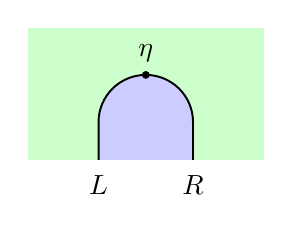
\begin{tikzpicture}[x=0.6cm,y=0.6cm, baseline=(current bounding box.center)]
        \begin{scope}       
            \clip (-2.5,0.2) rectangle (2.5,3);     
            \fill[fill=green!20] (-2.5,0.2) rectangle (2.5,3);  
            \draw[fill=blue!20, rounded corners=0.6cm, line width=0.7pt] (-1,-1) rectangle (1, 2); 
        \end{scope}
        \node[below=2pt] at (-1,0.2) {$L$};
        \node[below=2pt] at (1,0.2) {$R$};
        \node[above=1pt] at (0,2) {$\eta$};
        \draw[fill=black] (0, 2) circle (0.07);
    \end{tikzpicture}
\end{center}
defined by $\eta_X:=\Phi_{X,L(X)}\left(\mathrm{id}_{L(X)}\right)$ for any $X\in \mathrm{Ob}(\mathsf{C})$, where $\Phi_{X,L(X)}$ is the natural bijection
$$
\begin{aligned}
    \Phi_{X,L(X)}:\operatorname{Hom}_{\mathsf{D}}\left(L(X), L(X)\right) & \xlongrightarrow{\sim}\operatorname{Hom}_{\mathsf{C}}(X, RL(X)) \\
\operatorname{id}_{F(X)} & \longmapsto \eta_X 
\end{aligned}
$$
The \textbf{adjunction counit} $\varepsilon$ of this adjunction is a natural transformation
\begin{center}
    \begin{tikzcd}[ampersand replacement=\&]
        \mathsf{D} \arrow[r, "\scalebox{1.2}{$L\circ R$}"{name=A, above}, bend left=40] \arrow[r, "\scalebox{1.2}{$\mathrm{id}_{\mathsf{D}}$}"'{name=B, below}, bend right=40] 
        \&[+25pt] \mathsf{D}
        \arrow[Rightarrow, shorten <=3.5pt, shorten >=3.5pt, from=A.south-|B, to=B, "\varepsilon"]
    \end{tikzcd}
    \hspace{3cm}
    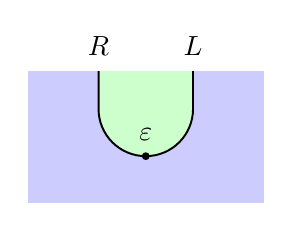
\begin{tikzpicture}[x=0.6cm,y=0.6cm, baseline=(current bounding box.center)]
        \begin{scope} 
            \clip (-2.5,0) rectangle (2.5,2.8);     
            \fill[fill=blue!20] (-2.5,0) rectangle (2.5,2.8);  
            \draw[fill=green!20, rounded corners=0.6cm, line width=0.7pt] (-1,1) rectangle (1, 4);
        \end{scope}
        \node[above=2pt] at (-1,2.8) {$R$};
        \node[above=2pt] at (1,2.8) {$L$};
        \node[above=2pt] at (0,1) {$\varepsilon$};
        \draw[fill=black] (0, 1) circle (0.07);  
    \end{tikzpicture}
\end{center}
defined by $\varepsilon_Y:=\Phi_{R(Y),Y}^{-1}\left(\mathrm{id}_{R(Y)}\right)$ for any $Y\in \mathrm{Ob}(\mathsf{D})$, where $\Phi_{R(Y),Y}^{-1}$ is the natural bijection
$$
\begin{aligned}
    \Phi_{R(Y),Y}^{-1}:\operatorname{Hom}_{\mathsf{D}}\left(R(Y), R(Y)\right) & \xlongrightarrow{\sim}\operatorname{Hom}_{\mathsf{C}}(LR(Y), R(Y)) \\
\mathrm{id}_{R(Y)} & \longmapsto \varepsilon_Y
\end{aligned}
$$
\end{definition}

\begin{prf}
    By naturality of $\Phi$, for any morphism $g:X_2\to X_1$ in $\mathsf{C}$, we have the following commutative diagram
    \[
    \begin{tikzcd}[ampersand replacement=\&]
        \mathrm{id}_{L(X_1)}\arrow[d,mapsto]\&[-30pt]\ni\&[-29pt]{\operatorname{Hom}_{\mathsf{D}}\left(L(X_1), L(X_1)\right) } \arrow[d, "{\Phi_{X_1,L(X_1)}}"'] \arrow[r,"{\left(L(g)\right)^*}"] \& [+12pt]{\operatorname{Hom}_{\mathsf{D}}\left(L(X_2), L(X_1)\right) } \arrow[d, "{\Phi_{X_2,L(X_1)}}"] \&[+12pt] {\operatorname{Hom}_{\mathsf{D}}\left(L(X_2), L(X_2)\right) } \arrow[d, "{\Phi_{X_2,L(X_2)}}"] \arrow[l,"{\left(L(g)\right)_*}"'] \&[-28pt]\in\&[-28pt]\mathrm{id}_{L(X_2)}\arrow[d,mapsto]\\[+20pt]
        \eta_{X_1}\&\ni\&{\operatorname{Hom}_{\mathsf{C}}(X_1, RL(X_1))} \arrow[r,"g^*"]                                                    \& {\operatorname{Hom}_{\mathsf{C}}(X_2, RL(X_1))}                                                   \& {\operatorname{Hom}_{\mathsf{C}}(X_2, RL(X_2))} \arrow[l, "\left(RL(g)\right)_*"']            \&[-30pt]\in\&[-30pt]\eta_{X_2}       
        \end{tikzcd}
        \]
        Since
        \[
        (L(g))^*\left(\mathrm{id}_{L(X_1)}\right)=L(g)=(L(g))_*\left(\mathrm{id}_{L(X_2)}\right),
        \]
        we have
        \[
        g^*(\eta_{X_1})=\Phi_{X_2,L(X_1)}(L(g))=\left(RL(g)\right)_*(\eta_{X_2}),
        \]   
    which implies the naturality square of $\eta$ commutes
\[
    \begin{tikzcd}[ampersand replacement=\&]
        X_2 \arrow[d, "{\eta_{X_2}}"'] \arrow[r, "g"] \&[+18pt]X_1\arrow[d, "{\eta_{X_1}}"]    \\[+15pt]
         RL(X_2)\arrow[r, "RL(g)"']\& RL(X_1)
    \end{tikzcd}
\] 
Similarly, we can show that for any morphism $h:Y_1\to Y_2$ in $\mathsf{D}$, the naturality square of $\varepsilon$ commutes
\[
    \begin{tikzcd}[ampersand replacement=\&]
        LR(Y_1) \arrow[d, "{\varepsilon_{Y_1}}"'] \arrow[r, "LR(h)"] \&[+18pt]LR(Y_2)\arrow[d, "{\varepsilon_{Y_2}}"]    \\[+15pt]
         Y_1\arrow[r, "h"']\& Y_2
    \end{tikzcd}
\]
\end{prf}

\begin{proposition}{Adjunction Isomorphism Determined by Unit or Counit}{}
    Let $\left(L,R,\Phi\right)$ be an adjoint pair of functors and $\eta$ and $\varepsilon$ be the adjunction unit and counit respectively. Then 
   \begin{align*}
\Phi_{X,Y}(f) & =R(f) \circ \eta_X: X \rightarrow R(Y), \quad \forall f: L(X) \rightarrow Y , \\
\Phi_{X,Y}^{-1}(g) & =\varepsilon_Y \circ L(g): L(X) \rightarrow Y, \quad \forall g: X \rightarrow R(Y) .
   \end{align*}
\end{proposition}

\begin{prf}
    For any object $X\in \mathrm{Ob}(\mathsf{C})$ and any morphism $f:L(X)\to Y$ in $\mathsf{D}$, we have the following commutative diagram
    \[
		\begin{tikzcd}[ampersand replacement=\&, row sep = 3.5em]
			\mathrm{id}_{L(X)}\arrow[d, mapsto]\&[-25pt]\in\&[-25pt]\mathrm{Hom}_{\mathsf{C}}(L(X),L(X)) \arrow[d, "{\Phi_{X,L(X)}}"']  \arrow[rr, "{f_*}"] \&[-15pt] \& {\mathrm{Hom}_{\mathsf{C}}(L(X),Y)}\arrow[d, "\Phi_{X,Y}"]\&[-25pt]\ni\&[-25pt]f \arrow[d, mapsto]\\
			\eta_X\&\in\&{\mathrm{Hom}_{\mathsf{C}}(X,RL(X))} \arrow[rr, "{\left(R(f)\right)_*}"'] \&  \& {\mathrm{Hom}_{\mathsf{C}}(X,R(Y))}  \&\ni\& \Phi_{X,Y}(f)     
		\end{tikzcd}
	\]
    For any object $Y\in \mathrm{Ob}(\mathsf{D})$ and any morphism $g:X\to R(Y)$ in $\mathsf{C}$, we have the following commutative diagram
    \[
        \begin{tikzcd}[ampersand replacement=\&, row sep = 3.5em]
            \mathrm{id}_{R(Y)}\arrow[d, mapsto]\&[-25pt]\in\&[-25pt]\mathrm{Hom}_{\mathsf{D}}(R(Y),R(Y)) \arrow[d, "{\Phi_{R(Y),Y}^{-1}}"']  \arrow[rr, "{g^*}"] \&[-15pt] \& {\mathrm{Hom}_{\mathsf{D}}(X,R(Y))}\arrow[d, "\Phi_{R(Y),Y}^{-1}"]\&[-25pt]\ni\&[-25pt]g \arrow[d, mapsto]\\
            \varepsilon_Y\&\in\&{\mathrm{Hom}_{\mathsf{C}}(LR(Y),Y)} \arrow[rr, "{\left(L(g)\right)^*}"'] \&  \& {\mathrm{Hom}_{\mathsf{C}}(L(X),Y)}  \&\ni\& \Phi_{X,Y}^{-1}(g)
        \end{tikzcd}
    \]
\end{prf}

\begin{lemma}{Snake Equations}{}
    Let $\left(L,R,\Phi\right)$ be an adjoint pair of functors and $\eta$ and $\varepsilon$ be the adjunction unit and counit respectively. Then we have the following equalities of natural transformations
    \begin{center}
        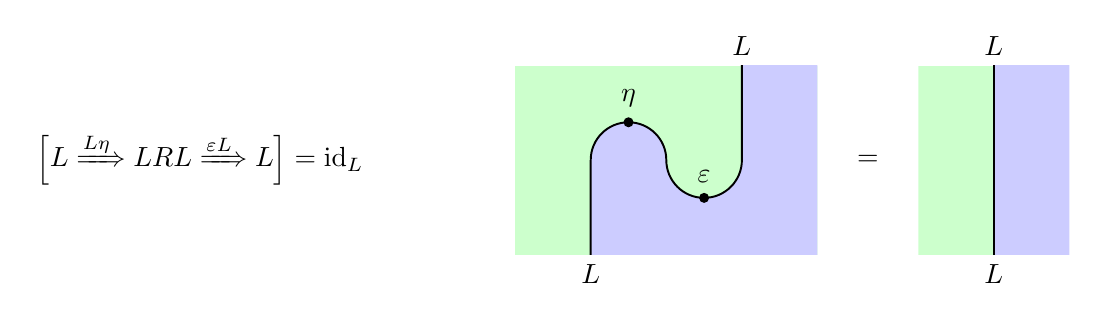
\begin{tikzpicture}[x=0.8cm,y=0.8cm]
            \node at (-7.4,1.5) {${\left[L \xRightarrow{L \eta}LR L\xRightarrow{\varepsilon L} L\right]=\mathrm{id}_L}$};
            \begin{scope} 
                \clip (-2.4,0) rectangle (2.4,3);     
                \fill[fill=green!20] (-2.5,0) rectangle (2.5,3);  
                \filldraw[fill=blue!20, rounded corners=0.48cm, line width=0.7pt] (-1.2,-1) -- (-1.2, 2.1)-- (0,2.1)-- (0,0.9)-- (1.2,0.9)
                   -- (1.2,4)-- (4,4)-- (4,-1)--cycle;
            \end{scope}
        
            \node[above] at (1.2,3) {$L$};
            \node[below] at (-1.2,0) {$L$};
        
            \draw[fill=black] (0.6, 0.9) circle (0.07);  
            \node[above=2pt] at (0.6, 0.9) {$\varepsilon$};
            
            \draw[fill=black] (-0.6, 2.1) circle (0.07); 
            \node[above=2pt] at (-0.6, 2.1) {$\eta$};
        
            \node at (3.2, 1.5) {$=$};
        
            \begin{scope} 
                \clip (4,0) rectangle (6.4,3); 
                \fill[fill=green!20] (4,0) rectangle (6.4,3); 
                \filldraw[fill=blue!20, line width=0.7pt] (5.2,-1) rectangle (7,4);  
            \end{scope} 
            
            \node[below] at (5.2,0) {$L$};
            \node[above] at (5.2,3) {$L$};
        \end{tikzpicture}
    \end{center}
    \begin{center}
        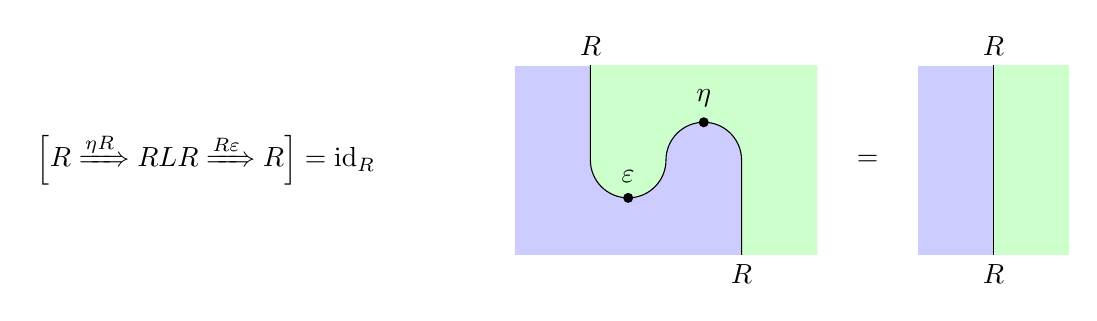
\begin{tikzpicture}[x=0.8cm,y=0.8cm]
            \node at (-7.3,1.5) {${\left[R \xRightarrow{\eta R}RLR \xRightarrow{R \varepsilon}R\right]=\mathrm{id}_R}$};
            \begin{scope} 
                \clip (-2.4, 0) rectangle (2.4, 3);     
                \fill[fill=blue!20] (-2.5, 0) rectangle (2.5,3);  
                \filldraw[fill=green!20, rounded corners=0.48cm] (-1.2, 4) -- (-1.2, 0.9)-- (0, 0.9)-- (0, 2.1)-- (1.2, 2.1)
                -- (1.2, -1)-- (4, -1)-- (4, 4)--cycle;
            \end{scope}
        
            \node[below] at (1.2,0) {$R$};
            \node[above] at (-1.2,3) {$R$};
        
            \draw[fill=black] (0.6, 2.1) circle (0.07);  
            \node[above=2pt] at (0.6, 2.1) {$\eta$};
            
            \draw[fill=black] (-0.6, 0.9) circle (0.07); 
            \node[above=2pt] at (-0.6, 0.9) {$\varepsilon$};
        
            \node at (3.2, 1.5) {$=$};
        
            \begin{scope} 
                \clip (4,0) rectangle (6.4,3); 
                \fill[fill=blue!20] (4,0) rectangle (6.4,3); 
                \filldraw[fill=green!20] (5.2,-1) rectangle (7,4);  
            \end{scope} 
            
            \node[below] at (5.2,0) {$R$};
            \node[above] at (5.2,3) {$R$};
        \end{tikzpicture}
    \end{center}
\end{lemma}

\begin{proposition}{}{}
    If $F:\mathsf{C}\to\mathsf{D}$ and $G:\mathsf{D}\to\mathsf{C}$ are inverse functors, which means $F\circ G=\mathrm{id}_{\mathsf{D}}$ and $G\circ F=\mathrm{id}_{\mathsf{C}}$, then we have $F\dashv G$ and $G\dashv F$.
\end{proposition}
\begin{prf}
    The snake equations of the adjunction unit and counit holds trivially because the unit $\eta:\mathrm{id}_{\mathsf{C}}\Rightarrow G\circ F$ and counit $\varepsilon:F\circ G\Rightarrow \mathrm{id}_{\mathsf{D}}$ are identity natural transformations.
\end{prf}

\begin{definition}{Wire Bending}{}
Let $\mathsf{C}$, $\mathsf{D}$, $\mathsf{C'}$, $\mathsf{D'}$ be categories and $L,R,L',R',H,K$ be functors shown in the following diagram
\[
    \begin{tikzcd}[ampersand replacement=\&]
        \mathsf{C} \arrow[dd, "L"', bend right=38] \arrow[r, "H"]  \&[+36pt] \mathsf{C'} \arrow[dd, "L'"', bend right=38] \\[-5pt]
        \dashv                                                  \& \dashv                                    \\[-5pt]
        \mathsf{D} \arrow[uu, "R"', bend right=38] \arrow[r, "K"'] \& \mathsf{D'} \arrow[uu, "R'"', bend right=38]
        \end{tikzcd}    
\]
There are bijections between the following sets of natural transformations
\[
    \begin{tikzcd}[ampersand replacement=\&]
        {\mathrm{Hom}_{[\mathsf{C}, \mathsf{D'}]}\left(L'H, KL\right) } \arrow[r, shift left=1pt, rightharpoonup, "\triangleright"]\arrow[r, shift right=1pt,leftharpoondown, "\triangleleft"']  \& {\mathrm{Hom}_{[\mathsf{C}, \mathsf{C'}]}(H, R'KL) } \arrow[d, shift left=1pt, rightharpoonup, "\triangleright"]\arrow[d, shift right=1pt,leftharpoondown, "\triangleleft"']   \\[+15pt]
        { \mathrm{Hom}_{[\mathsf{D}, \mathsf{D'}]}\left(L'HR, K\right)} \arrow[u, shift left=1pt, rightharpoonup, "\triangleright"]\arrow[u, shift right=1pt,leftharpoondown, "\triangleleft"'] \& {\mathrm{Hom}_{[\mathsf{D}, \mathsf{C'}]}(HR, R'K) } \arrow[l, shift left=1pt, rightharpoonup, "\triangleright"]\arrow[l, shift right=1pt,leftharpoondown, "\triangleleft"'] 
        \end{tikzcd}    
\]
natural in both $H$ and $K$ such that $\triangleleft=\triangleright^{-1}$ and $\triangleright\triangleright\triangleright\hspace{2.15pt}\triangleright=\triangleright^4=\mathrm{id}$. $\triangleright$ is called \textbf{wire bending} because its action can be visualized as bending the wires of adjoint pairs in the following string diagrams

\begin{center}
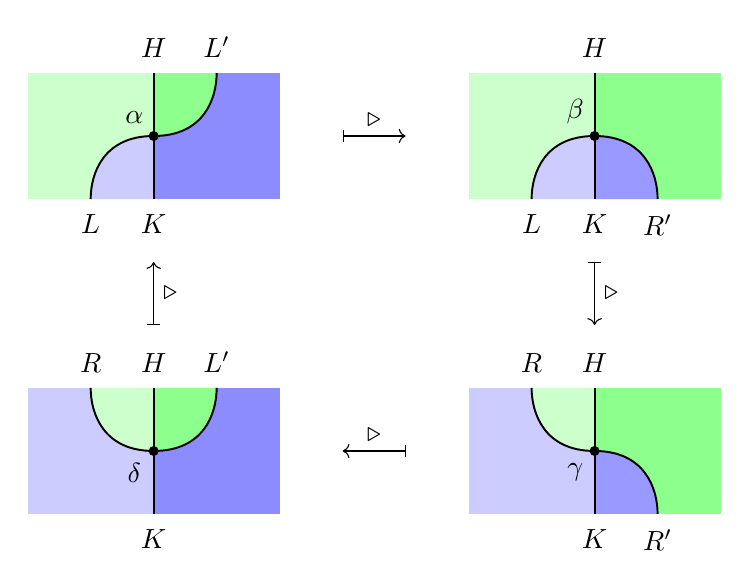
\begin{tikzpicture}[x=0.8cm,y=0.8cm, baseline=(current bounding box.center)]
    \draw [|-To] (3,1) -- (4,1) node[midway,above] {$\triangleright$};
    \draw [|-To] (7,-1) -- (7,-2) node[midway,right] {$\triangleright$};
    \draw [|-To] (4,-4) -- (3,-4) node[midway,above] {$\triangleright$};
    \draw [|-To] (0,-2) -- (0,-1) node[midway,right] {$\triangleright$};
    \begin{scope}      
        \fill[fill=green!20] (-2,0) rectangle (0,2);  
        \fill[fill=blue!45] (0,0) rectangle (2,2); 
        \fill[fill=blue!20] (-1,0) .. controls (-1,0.4) and (-0.8, 1) .. (0,1)--(0,0)--cycle;
        \fill[fill=green!45] (1,2) .. controls (1,1.6) and (0.8, 1) .. (0,1)--(0,2)--cycle;
    \end{scope}
    \draw[line width=0.7pt] (0,0) -- (0,2);
    \draw[line width=0.7pt] (-1,0) .. controls (-1, 0.4) and (-0.8, 1) .. (0, 1) .. controls (0.8, 1) and (1, 1.6) .. (1, 2);
    
    \node[above=2pt] at (0, 2) {$H$};
    \node[below=2pt] at (0, 0) {$K$};
    \node[below=2pt] at (-1, 0) {$L$};
    \node[above=2pt] at (1, 2) {$L'$};

    \draw[fill=black] (0, 1) circle (0.07);  
    \node[left=7pt, above=1pt] at (0, 1)  {$\alpha$};

\begin{scope}[shift={(7,0)}]
     \begin{scope}     
        \fill[fill=green!20] (-2,0) rectangle (0,2);  
        \fill[fill=green!45] (0,0) rectangle (2,2); 
        \fill[fill=blue!20] (-1,0) .. controls (-1, 0.4) and (-0.8, 1) .. (0,1)--(0,0)--cycle;
        \fill[fill=blue!40] (1,0) .. controls (1, 0.4) and (0.8, 1) .. (0,1)--(0,0)--cycle;
    \end{scope}
    \draw[line width=0.7pt] (0,0) -- (0,2);
    \draw[line width=0.7pt] (-1,0) .. controls (-1, 0.4) and (-0.8, 1) .. (0, 1) .. controls (0.8, 1) and (1, 0.4) .. (1, 0);
    
    \node[above=2pt] at (0, 2) {$H$};
    \node[below=2pt] at (0, 0) {$K$};
    \node[below=2pt] at (-1, 0) {$L$};
    \node[below=2pt] at (1, 0) {$R'$};

    \draw[fill=black] (0, 1) circle (0.07);  
    \node[left=7pt, above=1pt] at (0, 1)  {$\beta$};
\end{scope}
\begin{scope}[shift={(0,-5)}]
     \begin{scope}     
        \fill[fill=blue!20] (-2,0) rectangle (0,2);  
        \fill[fill=blue!45] (0,0) rectangle (2,2); 
        \fill[fill=green!20] (-1,2) .. controls (-1, 1.6) and (-0.8, 1) .. (0,1)--(0,2)--cycle;
        \fill[fill=green!45] (1,2) .. controls (1, 1.6) and (0.8, 1) .. (0,1)--(0,2)--cycle;
    \end{scope}
    \draw[line width=0.7pt] (0,0) -- (0,2);
    \draw[line width=0.7pt] (-1,2) .. controls (-1, 1.6) and (-0.8, 1) .. (0, 1) .. controls (0.8, 1) and (1, 1.6) .. (1, 2);
    
    \node[above=2pt] at (0, 2) {$H$};
    \node[below=2pt] at (0, 0) {$K$};
    \node[above=2pt] at (-1, 2) {$R$};
    \node[above=2pt] at (1, 2) {$L'$};

    \draw[fill=black] (0, 1) circle (0.07);  
    \node[left=7pt, below=1pt] at (0, 1)  {$\delta$};
\end{scope}
\begin{scope}[shift={(7,-5)}]
     \begin{scope}     
        \fill[fill=blue!20] (-2,0) rectangle (0,2);  
        \fill[fill=green!45] (0,0) rectangle (2,2); 
        \fill[fill=green!20] (-1,2) .. controls (-1, 1.6) and (-0.8, 1) .. (0,1)--(0,2)--cycle;
        \fill[fill=blue!40] (1,0) .. controls (1, 0.4) and (0.8, 1) .. (0,1)--(0,0)--cycle;
    \end{scope}
    \draw[line width=0.7pt] (0,0) -- (0,2);
    \draw[line width=0.7pt] (-1,2) .. controls (-1, 1.6) and (-0.8, 1) .. (0, 1) .. controls (0.8, 1) and (1, 0.4) .. (1, 0);
    
    \node[above=2pt] at (0, 2) {$H$};
    \node[below=2pt] at (0, 0) {$K$};
    \node[above=2pt] at (-1, 2) {$R$};
    \node[below=2pt] at (1, 0) {$R'$};

    \draw[fill=black] (0, 1) circle (0.07);  
    \node[left=7pt, below=1pt] at (0, 1)  {$\gamma$};
\end{scope}
\end{tikzpicture}
\end{center}
\end{definition}

We only explicit define $\alpha^\triangleright$ here. The other wire bendings are defined similarly using the unit or counit of the adjunctions.
\begin{center} 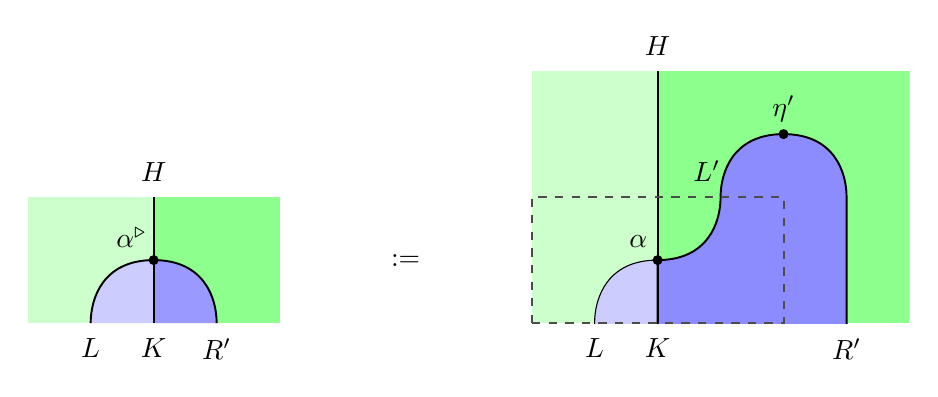
\begin{tikzpicture}[x=0.8cm,y=0.8cm, baseline=(current bounding box.center)]
    \begin{scope}     
        \fill[fill=green!20] (-2,0) rectangle (0,2);  
        \fill[fill=green!45] (0,0) rectangle (2,2); 
        \fill[fill=blue!20] (-1,0) .. controls (-1, 0.4) and (-0.8, 1) .. (0,1)--(0,0)--cycle;
        \fill[fill=blue!40] (1,0) .. controls (1, 0.4) and (0.8, 1) .. (0,1)--(0,0)--cycle;
    
    \draw[line width=0.7pt] (0,0) -- (0,2);
    \draw[line width=0.7pt] (-1,0) .. controls (-1, 0.4) and (-0.8, 1) .. (0, 1) .. controls (0.8, 1) and (1, 0.4) .. (1, 0);
    
    \node[above=2pt] at (0, 2) {$H$};
    \node[below=2pt] at (0, 0) {$K$};
    \node[below=2pt] at (-1, 0) {$L$};
    \node[below=2pt] at (1, 0) {$R'$};

    \draw[fill=black] (0, 1) circle (0.07);  
    \node[left=8pt, above=1pt] at (0, 1)  {$\alpha^{\triangleright}$};
    \end{scope}
    
    \node at (4, 1) {$:=$};
    
    \begin{scope} [shift={(8,0)}]
    \begin{scope} 
            \clip (-2,0) rectangle (4,4);     
            \fill[fill=green!20] (-2,0) rectangle (0,4);  
            \fill[fill=green!45] (0,0) rectangle (4,4);  
            \filldraw[fill=blue!20] (-1,-1) -- (-1,0) .. controls (-1,0.4) and (-0.8, 1) .. (0,1)--(0,-1)--cycle;
            \filldraw[fill=blue!45, line width=0.7pt] (0, -1) -- 
            (0, 1) .. controls (0.8, 1) and (1, 1.6) ..  
            (1, 2) .. controls (1, 2.4) and (1.2, 3) .. 
            (2, 3) .. controls (2.8, 3) and (3, 2.4) .. 
            (3, 2)--(3, -1)--cycle;
    \end{scope}
        \draw[line width=0.7pt] (0,0) -- (0,4);

        \node[above=2pt] at (0, 4) {$H$};
        \node[below=2pt] at (0, 0) {$K$};
        \node[below=2pt] at (-1, 0) {$L$};
        \node[left=5pt,above=2pt] at (1, 2) {$L'$};
        \node[below=2pt] at (3, 0) {$R'$};
    
        \draw[fill=black] (0, 1) circle (0.07);  
        \node[left=7pt, above=1pt] at (0, 1)  {$\alpha$};

        \draw[fill=black] (2, 3) circle (0.07);  
        \node[above=1pt] at (2, 3)  {$\eta'$};

        \draw[dashed, color=black!70, line width=0.7pt] (-2,0) rectangle (2,2);
    \end{scope}
    \end{tikzpicture}    
\end{center}
The fact that $\triangleleft$ is the inverse of $\triangleright$ follows from the snake equations.


\begin{proposition}{Equivalent Definition of Adjoint Functor Using Unit and Counit}{}
    Given pair of functors $\begin{tikzcd}[ampersand replacement=\&]
        \mathsf{C} \arrow[r, "L", bend left] \& \mathsf{D} \arrow[l, "R", bend left]
        \end{tikzcd}$
    there is a bijection between the following sets 
    \begin{align*}
        T:\left\{\text{adjoint pair }\left(L,R,\Phi\right)\right\}&\xrightleftharpoons{\;\sim\;}\left\{\left(L,R,\eta,\varepsilon\right)\text{ that satisfies snake equations}\right\}\\
        \Phi&\longmapsto\left(\eta_X:=\Phi\left(\mathrm{id}_{L(X)}\right), \varepsilon_Y:=\Phi^{-1}\left(\mathrm{id}_{R(Y)}\right)\right)\\
        \Phi_{X,Y}(f):=R(f) \circ \eta_X&\longmapsfrom(\eta, \varepsilon)
    \end{align*}
\end{proposition}

\begin{prf}
    Suppose $\left(L,R,\eta,\varepsilon\right)$ satisfies snake equations. Consider the diagram
    \[
        \begin{tikzcd}[ampersand replacement=\&]
            \boldone \arrow[dd, "\mathrm{id}"', bend right=38] \arrow[r, "\diagfunctor X"]  \&[+36pt] \mathsf{C} \arrow[dd, "L"', bend right=38] \\[-5pt]
            \dashv                                                  \& \dashv                                    \\[-5pt]
            \boldone \arrow[uu, "\mathrm{id}"', bend right=38] \arrow[r, "\diagfunctor Y"'] \& \mathsf{D} \arrow[uu, "R"', bend right=38]
            \end{tikzcd}    
    \]

    \begin{center}
        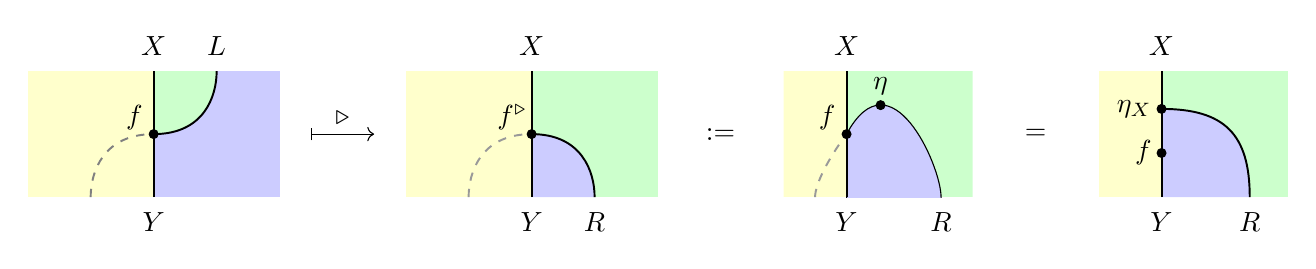
\begin{tikzpicture}[x=0.8cm,y=0.8cm, baseline=(current bounding box.center)]
        \definecolor{leftcolor}{RGB}{255,255,204}
            \draw [|-To] (2.5,1) -- (3.5,1) node[midway,above] {$\triangleright$};
            \node at (9, 1) {$:=$};
            \node at (14, 1) {$=$};
          
            \begin{scope}     
                \fill[fill=leftcolor] (-2,0) rectangle (0,2);  
                \fill[fill=blue!20] (0,0) rectangle (2,2); 
                \fill[fill=green!20] (1,2) .. controls (1,1.6) and (0.8, 1) .. (0,1)--(0,2)--cycle;
            \end{scope}
            \draw[line width=0.7pt] (0,0) -- (0,2);
            \draw[dashed, color=black!50, line width=0.7pt] (-1,0) .. controls (-1, 0.4) and (-0.8, 1) .. (0, 1) ;
            \draw[line width=0.7pt]  (0, 1) .. controls (0.8, 1) and (1, 1.6) .. (1, 2);
            
            \node[above=2pt] at (0, 2) {$X$};
            \node[below=2pt] at (0, 0) {$Y$};
            \node[above=2pt] at (1, 2) {$L$};
        
            \draw[fill=black] (0, 1) circle (0.07);  
            \node[left=7pt, above=-2pt] at (0, 1)  {$f$};
        
        \begin{scope}[shift={(6,0)}]
             \begin{scope} 
                    
                \fill[fill=leftcolor] (-2,0) rectangle (0,2);  
                \fill[fill=green!20] (0,0) rectangle (2,2); 
              
                \fill[fill=blue!20] (1,0) .. controls (1, 0.4) and (0.8, 1) .. (0,1)--(0,0)--cycle;
            \end{scope}
            \draw[line width=0.7pt] (0,0) -- (0,2);
            \draw[dashed, color=black!40, line width=0.7pt] (-1,0) .. controls (-1, 0.4) and (-0.8, 1) .. (0, 1);
            \draw[line width=0.7pt] (0, 1) .. controls (0.8, 1) and (1, 0.4) .. (1, 0);
            \node[above=2pt] at (0, 2) {$X$};
            \node[below=2pt] at (0, 0) {$Y$};
            \node[below=2pt] at (1, 0) {$R$};
        
            \draw[fill=black] (0, 1) circle (0.07);  
            \node[left=7pt, above=-2pt] at (0, 1)  {$f^{\hspace{0.2pt}\triangleright}$};
        \end{scope}
      \begin{scope}[shift={(11,0)}]
             \begin{scope} 
                \clip (-1,0) rectangle (2,2);     
                \fill[fill=leftcolor] (-2,0) rectangle (0,2);  
                \fill[fill=green!20] (0,0) rectangle (2,2); 
                \filldraw[fill=blue!20] (1.5,-1)--(1.5,0) .. controls (1.5, 0.5) and (0.7, 2.3) .. (0,1)--(0,-1)--cycle;
            \end{scope}
            \draw[line width=0.7pt] (0,0) -- (0,2);
            \draw[dashed, color=black!40, line width=0.7pt] (-0.5,0) .. controls (-0.5, 0.2) and (-0.3, 0.6) .. (0, 1);
            \node[above=2pt] at (0, 2) {$X$};
            \node[below=2pt] at (0, 0) {$Y$};
            \node[below=2pt] at (1.5, 0) {$R$};
        
            \draw[fill=black] (0, 1) circle (0.07);  
            \draw[fill=black] (0.54, 1.46) circle (0.07) node[above=0pt] {$\eta$}; 
            \node[left=7pt, above=-2pt] at (0, 1)  {$f$};
        \end{scope}

        \begin{scope}[shift={(16,0)}]
             \begin{scope}     
                \fill[fill=leftcolor] (-1,0) rectangle (0,2);  
                \fill[fill=green!20] (0,0) rectangle (2,2); 
         
                \fill[fill=blue!20] (1.4,0) .. controls (1.4,1) and (1, 1.4) .. (0,1.4)--(0,0)--cycle;
            \end{scope}
            \draw[line width=0.7pt] (0,0) -- (0,2);
         
            \draw[line width=0.7pt] (0, 1.4) .. controls (1, 1.4) and (1.4, 1) .. (1.4, 0);
            \node[above=2pt] at (0, 2) {$X$};
            \node[below=2pt] at (0, 0) {$Y$};
            \node[below=2pt] at (1.4, 0) {$R$};
        
            \draw[fill=black] (0, 0.7) circle (0.07) node[left=0pt] {$f$};  
            \draw[fill=black] (0, 1.4) circle (0.07) node[left=0pt] {$\eta_X$};  
        \end{scope}
        
        \end{tikzpicture}
    \end{center}
    As the string diagram shows, we find $\Phi_{X,Y}$ conincides with the wire bending map
    \[
        \triangleright: \mathrm{Hom}_{\mathsf{D}}\left(L(X), Y\right)\xlongrightarrow{\sim} \mathrm{Hom}_{\mathsf{C}}(X, R(Y)) 
    \]
    which is natural in both $X$ and $Y$. Hence $\Phi$ is a natural isomorphism. It is straightforward to check that $T$ is a bijection.
\end{prf}


\begin{proposition}{Uniqueness of Adjunction}{}
    If $\left(L,R,\eta,\varepsilon\right)$ and $\left(L,R',\eta', \varepsilon\right)$ are two adjoint pairs of functors, then there is a unique natural isomorphism $\psi:R\xRightarrow{\sim} R'$ such that 
    \[
        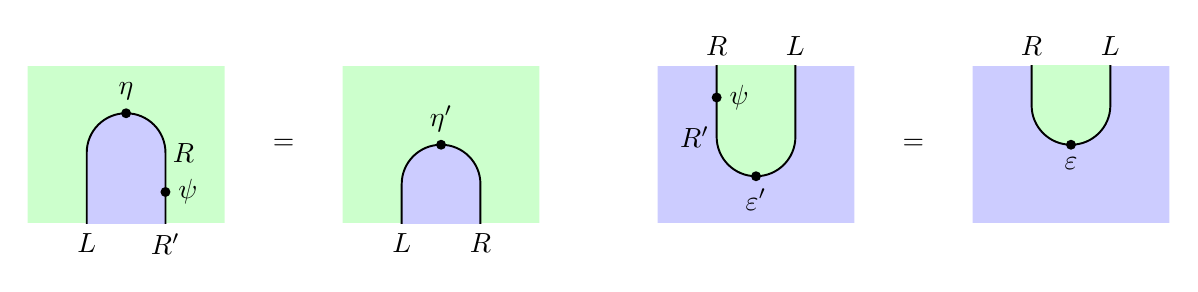
\begin{tikzpicture}[x=0.5cm,y=0.5cm,line width=0.7pt,hollow/.style={
                   circle,
                   fill=white,
                   draw,
                   outer sep=0pt,
                   inner sep=1.7pt,
                   line width=0.7pt
                 }]
           \definecolor{leftcolor}{RGB}{204, 255, 204}
           \definecolor{midcolor}{RGB}{204, 204, 255}
           
       
           \node at (4, 2) {$=$};
          \node at (20, 2) {$=$};
           
           
            \begin{scope}
               \begin{scope} 
                   \clip (-2.5,0) rectangle (2.5, 4);     
                   \fill[fill=leftcolor] (-3,0) rectangle (3, 4);  
                    
                   \draw[fill=midcolor, rounded corners=0.5cm, line width=0.7pt] (-1, -2) rectangle (1, 2.8);
               \end{scope}
             
               \filldraw [black] (1,0.8) circle (0.1) node[right=1pt] {$\psi$};
               \node[below] at (-1, 0) {$L$};
               \node[right=-1pt] at (1, 1.8) {$R$};
               \node[below] at (1, 0) {$R'$};
               \draw[fill=black] (0, 2.8) circle (0.1);
               \node[above=1pt] at (0, 2.8) {$\eta$}; 
             
           \end{scope}
           
           \begin{scope}[shift={(8,0)}]
               \begin{scope} 
                   \clip (-2.5,0) rectangle (2.5, 4); 
                   \fill[fill=leftcolor] (-3,0) rectangle (3, 4);  
                   \draw[fill=midcolor, rounded corners=0.5cm, line width=0.7pt] (-1, -2) rectangle (1, 2);
               \end{scope}
               \node[below] at (-1, 0) {$L$};
               \node[below] at (1, 0) {$R$};
               \draw[fill=black] (0, 2) circle (0.1);
               \node[above=1pt] at (0, 2) {$\eta'$}; 
           
           \end{scope}
           
           \begin{scope}[shift={(16,0)}]
               \begin{scope} 
                   \clip (-2.5,0) rectangle (2.5, 4);     
                   \fill[fill=midcolor] (-3,0) rectangle (3, 4);  
                    
                   \draw[fill=leftcolor, rounded corners=0.5cm, line width=0.7pt] (-1, 6) rectangle (1, 1.2);
               \end{scope}
             
               \filldraw [black] (-1,3.2) circle (0.1) node[right=1pt] {$\psi$};
               \node[above] at (-1, 4) {$R$};
               \node[left=-1pt] at (-1, 2.2) {$R'$};
               \node[above] at (1, 4) {$L$};
               \draw[fill=black] (0, 1.2) circle (0.1);
               \node[below=1pt] at (0, 1.2) {$\varepsilon'$}; 
             
           \end{scope}
           
           \begin{scope}[shift={(24,0)}]
               \begin{scope} 
                   \clip (-2.5,0) rectangle (2.5, 4); 
                   \fill[fill=midcolor] (-3,0) rectangle (3, 4);  
                   \draw[fill=leftcolor, rounded corners=0.5cm, line width=0.7pt] (-1, 6) rectangle (1, 2);
               \end{scope}
               \node[above] at (1, 4) {$L$};
               \node[above] at (-1, 4) {$R$};
               \draw[fill=black] (0, 2) circle (0.1);
               \node[below=1pt] at (0, 2) {$\varepsilon$}; 
           
           \end{scope}
           
        \end{tikzpicture}
    \]
\end{proposition}

\begin{prf}
    Consider the diagram
    \[
        \begin{tikzcd}[ampersand replacement=\&]
            \mathsf{C} \arrow[dd, "L"', bend right=38] \arrow[r, "\mathrm{id}_{\mathsf{C}}"]  \&[+36pt] \mathsf{C} \arrow[dd, "L"', bend right=38] \\[-5pt]
            \dashv                                                  \& \dashv                                    \\[-5pt]
            \mathsf{D} \arrow[uu, "R"', bend right=38] \arrow[r, "\mathrm{id}_{\mathsf{D}}"'] \& \mathsf{D} \arrow[uu, "R'"', bend right=38]
            \end{tikzcd}    
    \]
    Define $\psi:=\mathrm{id}_L^{\:\triangleright\triangleright}$, which is illustrated by the following string diagram
    \begin{center}
        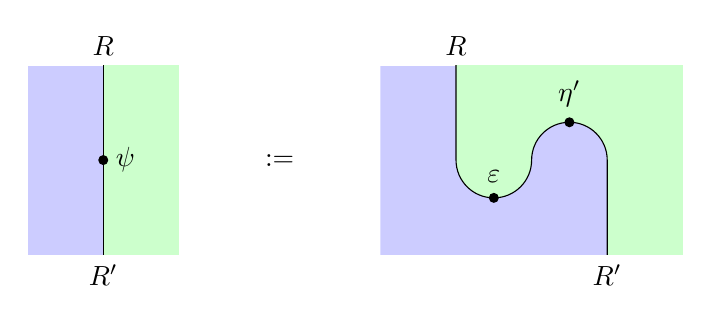
\begin{tikzpicture}[x=0.8cm,y=0.8cm]
            \node at (8, 1.5) {$:=$};
            \begin{scope}
                \begin{scope} 
                    \clip (4,0) rectangle (6.4,3); 
                    \fill[fill=blue!20] (4,0) rectangle (6.4,3); 
                    \filldraw[fill=green!20] (5.2,-1) rectangle (7,4);  
                \end{scope} 
                \draw[fill=black] (5.2, 1.5) circle (0.07) node[right=1pt] {$\psi$};
                \node[below] at (5.2,0) {$R'$};
                \node[above] at (5.2,3) {$R$};
            \end{scope}
            \begin{scope}[shift={(12,0)}] 
                \begin{scope}
                    \clip (-2.4, 0) rectangle (2.4, 3);     
                    \fill[fill=blue!20] (-2.5, 0) rectangle (2.5,3);  
                    \filldraw[fill=green!20, rounded corners=0.48cm] (-1.2, 4) -- (-1.2, 0.9)-- (0, 0.9)-- (0, 2.1)-- (1.2, 2.1)
                    -- (1.2, -1)-- (4, -1)-- (4, 4)--cycle;
                \end{scope}
        
                \node[below] at (1.2,0) {$R'$};
                \node[above] at (-1.2,3) {$R$};
            
                \draw[fill=black] (0.6, 2.1) circle (0.07);  
                \node[above=2pt] at (0.6, 2.1) {$\eta'$};
                
                \draw[fill=black] (-0.6, 0.9) circle (0.07); 
                \node[above=2pt] at (-0.6, 0.9) {$\varepsilon$};
              
            \end{scope}   
        \end{tikzpicture}
    \end{center}
    $\psi$ is a natural isomorphism since it has inverse $\mathrm{id}_L^{\:\triangleleft\triangleleft}$. The first equality in the statement of the proposition follows from $\psi^{\triangleleft}=\psi^{\triangleright\triangleright\triangleright}=\mathrm{id}_L^{\:\triangleright}=\eta'$. The uniqueness of $\psi$ follows from the injectivity of 
    $$
    \triangleleft:\mathrm{Hom}_{\left[\mathsf{D},\mathsf{C}\right]}\left(R,R'\right)\xlongrightarrow{\sim} \mathrm{Hom}_{\left[\mathsf{C},\mathsf{C}\right]}\left(\mathrm{id}_{\mathsf{C}},R'L\right).
    $$
    Similarly, the second equality follows from $\psi^{\triangleright}=\psi^{\triangleleft\triangleleft\triangleleft}=\mathrm{id}_L^{\:\triangleleft}=\varepsilon$. And the uniqueness of $\psi$ follows from the injectivity of
    $$
    \triangleright:\mathrm{Hom}_{\left[\mathsf{C},\mathsf{D}\right]}\left(L',L\right)\xlongrightarrow{\sim} \mathrm{Hom}_{\left[\mathsf{D},\mathsf{D}\right]}\left(LR,\mathrm{id}_{\mathsf{D}}\right).
    $$
\end{prf}



\begin{proposition}{Equivalent Definition of Adjoint Functor Using Representable Functor}{adjunction_by_representability}
    \begin{enumerate}[(i)]
        \item A functor $L:\mathsf{C}\to\mathsf{D}$ has right adjoint if and only for each $Y\in \mathrm{Ob}(\mathsf{D})$, $\mathrm{Hom}_{\mathsf{D}}\left(L(-),Y\right)$ is representable. If so, the universal element of $\mathrm{Hom}_{\mathsf{D}}\left(L(-),Y\right)$ is $\left(R(Y), \varepsilon_Y\right)$.
        \item A functor $R:\mathsf{D}\to\mathsf{C}$ has left adjoint if and only for each $X\in \mathrm{Ob}(\mathsf{C})$, $\mathrm{Hom}_{\mathsf{C}}\left(X,R(-)\right)$ is representable. If so, the universal element of $\mathrm{Hom}_{\mathsf{C}}\left(X,R(-)\right)$ is $\left(L(X), \eta_X\right)$.
    \end{enumerate}
\end{proposition}

\begin{prf}
    We only prove (i) here. The proof of (ii) is similar. 
    If $(L, R, \Phi)$ is an adjoint pair of functors, then for each $Y\in \mathrm{Ob}(\mathsf{D})$, we have an isomorphism 
    $$
    \Phi_{\text{-},Y}:\mathrm{Hom}_{\mathsf{D}}\left(L(-),Y\right)\xRightarrow{\sim} \mathrm{Hom}_{\mathsf{D}}\left(-,R(Y)\right).
    $$
    where $\Phi_{\text{-},Y}$ is the horizontal composition
    \[
        \begin{tikzcd}[ampersand replacement=\&]
            \mathsf{C}^{\mathrm{op}}\times\boldone\arrow[r,"{\mathrm{id}\times\diagfunctor Y}"]\&[+15pt]\mathsf{C}^{\mathrm{op}}\times\mathsf{D} \arrow[r, "\scalebox{1.2}{$\mathrm{Hom}_{\mathsf{D}}\left(L(-){,}-\right)$}"{name=A, above}, bend left] \arrow[r, "\scalebox{1.2}{$\mathrm{Hom}_{\mathsf{C}}\left(-{,}R(-)\right)$}"'{name=B, below}, bend right] \&[+60pt] \mathsf{Set}
            \arrow[Rightarrow, shorten <=5.5pt, shorten >=5.5pt, from=A.south-|B, to=B, "\Phi", "\sim\hspace{1.5pt}"']
        \end{tikzcd}
\]
    Since 
    \[
        \left(\Phi_{-,Y}^{-1}\right)_{R(Y)}\left(\mathrm{id}_{R(Y)}\right)=\Phi_{R(Y),Y}^{-1}\left(\mathrm{id}_{R(Y)}\right)=\varepsilon_Y,
    \]
    we see $\mathrm{Hom}_{\mathsf{D}}\left(L(-),Y\right)$ is representable by $\left(R(Y), \varepsilon_Y\right)$.

    Conversely, suppose for each $Y\in \mathrm{Ob}(\mathsf{D})$, $\mathrm{Hom}_{\mathsf{D}}\left(L(-),Y\right)$ is representable. Then for each $Y\in \mathrm{Ob}(\mathsf{D})$, there exist a natural isomorphism 
    $$
    \phi(Y):\mathrm{Hom}_{\mathsf{D}}\left(-,R_Y\right)\xRightarrow{\sim} \mathrm{Hom}_{\mathsf{D}}\left(L(-),Y\right)
    $$
    for some $R_Y\in \mathrm{Ob}(\mathsf{D})$. \Cref{th:representable_functor_by_universal_element} implies that $(R_Y,\phi(Y))$ is terminal in the category $\left(Y_{\mathsf{C}}\downarrow \mathrm{Hom}_{\mathsf{D}}\left(L(-),Y\right)\right)$, which corresponds to 
    $$ 
    \begin{tikzcd}[ampersand replacement=\&]
        \mathsf{C} \arrow[r, " Y_{\mathsf{C}}"] \& \left[\mathsf{C}^{\mathrm{op}},\mathsf{Set}\right] \&[+45pt]  \boldone \arrow[l, "{\diagfunctor \mathrm{Hom}_{\mathsf{D}}\left(L(-),Y\right)}"']
    \end{tikzcd}
    $$ 
    Given any morphism $h:Y_1\to Y_2$ in $\mathsf{D}$, since $(R_{Y_2},\phi(Y_2))$ is terminal in $\left(Y_{\mathsf{C}}\downarrow \mathrm{Hom}_{\mathsf{D}}\left(L(-),Y\right)\right)$, there exists a unique morphism $R_h:R_{Y_1}\to R_{Y_2}$  in $\mathsf{C}$ such that the following diagram commutes
     \[
     \begin{tikzcd}[ampersand replacement=\&]
        Y_{\mathsf{C}}\left(R_{Y_1}\right) \arrow[d, "Y_{\mathsf{C}}(R_h)"', dashed] \arrow[r, "\phi\left(Y_1\right)"] \&[+10pt] {\mathrm{Hom}_{\mathsf{D}}\left(L(-),Y_1\right)} \arrow[d, "h_\star"] \\[+15pt]
        Y_{\mathsf{C}}\left(R_{Y_2}\right) \arrow[r, "\phi\left({Y_2}\right)"']                                                   \& {\mathrm{Hom}_{\mathsf{D}}\left(L(-),Y_2\right)}                 
    \end{tikzcd}\hspace{3em}=\hspace{3em}
    \begin{tikzcd}[ampersand replacement=\&]
        \mathrm{Hom}_{\mathsf{C}}\left(-,R_{Y_1}\right)\arrow[d, "\left(R_h\right)_\star"', dashed] \arrow[r, "\phi\left(Y_1\right)"] \&[+10pt] {\mathrm{Hom}_{\mathsf{D}}\left(L(-),Y_1\right)} \arrow[d, "h_\star"] \\[+15pt]
        \mathrm{Hom}_{\mathsf{C}}\left(-,R_{Y_2}\right) \arrow[r, "\phi\left({Y_2}\right)"']                                                   \& {\mathrm{Hom}_{\mathsf{D}}\left(L(-),Y_2\right)}                 
    \end{tikzcd}
    \]
    Thus we can define a functor $R:\mathsf{D}\to\mathsf{C}$ by $R(Y):=R_Y$ and $R(h):= R_h$. We can also define a natural isomorphism $\Phi: \mathrm{Hom}_{\mathsf{D}}\left(L(-),-\right)\xRightarrow{\sim} \mathrm{Hom}_{\mathsf{D}}\left(-,R(-)\right)$ by
    \begin{align*}
        \Phi_{X,Y}:\mathrm{Hom}_{\mathsf{D}}\left(L(X),Y\right)&\xlongrightarrow{\sim} \mathrm{Hom}_{\mathsf{C}}\left(X,R(Y)\right)\\
        \Big(L(X)\xlongrightarrow{f}Y\Big)&\longmapsto \Big(X\xlongrightarrow{\left(\phi(Y)_X\right)^{-1}(f)}R(Y)\Big)
    \end{align*}
    The naturality of $\Phi$ can be check as follows: for any morphism $g:X_2\to X_1$ in $\mathsf{C}$ and $h:Y_1\to Y_2$ in $\mathsf{D}$, the following diagram commutes
    \[
        \begin{tikzcd}[ampersand replacement=\&]
            \mathrm{Hom}_{\mathsf{D}}\left(L(X_1),Y_1\right) \arrow[r, "L(g)^*"] \arrow[d, "\Phi_{X_1,Y_1}"', "\left(\phi(Y_1)_{X_1}\right)^{-1}"] \&[+40pt]\mathrm{Hom}_{\mathsf{D}}\left(L(X_2),Y_1\right) \arrow[r, "{h_*}"]\arrow[d, "\Phi_{X_2,Y_1}"', "\left(\phi(Y_1)_{X_2}\right)^{-1}"] \&[+40pt] \mathrm{Hom}_{\mathsf{D}}\left(L(X_2),Y_2\right) \arrow[d, "\Phi_{X_2,Y_2}"', "\left(\phi(Y_2)_{X_2}\right)^{-1}"] \\[+20pt]
            \mathrm{Hom}_{\mathsf{C}}\left(X_1,R(Y_1)\right) \arrow[r, "{g^*}"'] \&\mathrm{Hom}_{\mathsf{C}}\left(X_2,R(Y_1)\right) \arrow[r, "{R(h)_*}"']\& \mathrm{Hom}_{\mathsf{C}}\left(X_2,R(Y_2)\right)
        \end{tikzcd}
    \]
    Therefore, $(L,R,\Phi)$ is an adjoint pair of functors.
\end{prf}


\begin{corollary}{Equivalent Definition of Adjoint Functor Using Universal Morphism}{}
    Given pair of functors $\begin{tikzcd}[ampersand replacement=\&]
        \mathsf{C} \arrow[r, "L", bend left] \& \mathsf{D} \arrow[l, "R", bend left]
        \end{tikzcd}$, then the following are equivalent
    \begin{enumerate}[(i)]
        \item $L \dashv R$.
        \item For every object $X\in\mathrm{Ob}(\mathsf{C})$, there exists $\left(L(X), X\xrightarrow{\eta_X} R(L(X))\right)$ initial in $\left(X\downarrow R\right)$, i.e. there exists a \hyperref[th:universal_morphism]{universal morphism} from $X$ to $R$.
        \item For every object $Y\in\mathrm{Ob}(\mathsf{D})$, there exists $\left(R(Y), L(R(Y))\xrightarrow{\varepsilon_Y} Y\right)$ terminal in $\left(L\downarrow Y\right)$, i.e. there exists a \hyperref[th:universal_morphism]{universal morphism} from $L$ to $Y$.
    \end{enumerate} 
\end{corollary}

\begin{prf}
    This is a direct consequence of \Cref{th:adjunction_by_representability}. According to \Cref{th:universal_morphism_by_representability}, for each $X\in\mathrm{Ob}(\mathsf{C})$, $\mathrm{Hom}_{\mathsf{C}}\left(X,R(-)\right)$ is representable by $\left(L(X),\eta_X\right)$ is equivalent to that $\left(L(X), X\xrightarrow{\eta_X} R(L(X))\right)$ is initial in $\left(X\downarrow R\right)$.

    \[
        \begin{tikzcd}[ampersand replacement=\&]
            X \arrow[r, "\eta_X"] \arrow[rd, "g"'] \&[+20pt] R(L(X)) \arrow[d, "R\left(g^{\triangleleft}\right)", dashed] \&[+50pt]    \{*\} \arrow[r, "\diagfunctor \eta_X"] \arrow[rd, "\diagfunctor g"'] \&[+15pt] \mathrm{Hom}_{\mathsf{C}}\left(X,R(L(X))\right) \arrow[d, "R\left(g^{\triangleleft}\right)_*", dashed] \\[+20pt]
            \& R(Y) \&\& \mathrm{Hom}_{\mathsf{C}}\left(X,R(Y)\right)     
        \end{tikzcd}
    \]

    Similarly, for each $Y\in\mathrm{Ob}(\mathsf{D})$, $\mathrm{Hom}_{\mathsf{D}}\left(L(-),Y\right)$ is representable by $\left(R(Y), \varepsilon_Y\right)$ is equivalent to that $\left(R(Y), \varepsilon_Y\right)$ is terminal in $\left(L\downarrow Y\right)$.
    \[
        \begin{tikzcd}[ampersand replacement=\&]
            L(X) \arrow[d, "L\left(f^{\triangleright}\right)"', dashed] \arrow[rd, "f"] \&[+20pt]   \&[+50pt]   {\mathrm{Hom}_{\mathsf{D}}\left(L(X),Y\right)}     \&[+15pt]  \\[+20pt]
            L(R(Y)) \arrow[r, "\eta_Y"']   \& Y \&  {\mathrm{Hom}_{\mathsf{D}}\left(L(R(Y)),Y\right)} \arrow[u, "L\left(f^{\triangleright}\right)^*", dashed] \& \{*\} \arrow[lu, "\diagfunctor f"'] \arrow[l, "\diagfunctor\eta_Y"]
        \end{tikzcd}
    \]
\end{prf}



\section{Kan Extension}

\begin{definition}{Kan Extension}{}
    Let $\mathsf{C}$, $\mathsf{D}$, $\mathsf{E}$ be categories and $K:\mathsf{C}\to\mathsf{D}$, $F:\mathsf{C}\to\mathsf{E}$ be functors. A \textbf{left Kan extension} of $F$ along $K$ is a pair $\left(\mathrm{Lan}_KF,\eta\right)$ consisting of
    \begin{itemize}
        \item a functor $\mathrm{Lan}_KF:\mathsf{D}\to\mathsf{E}$,
        \item a natural transformation $\eta:F\Rightarrow \left(\mathrm{Lan}_KF\right)\circ K$
    \end{itemize}
    \begin{center}
        \begin{tikzcd}[ampersand replacement=\&, column sep=3em] 
            % drawing 0- and 1-celss 
            \mathsf{C} \arrow[dr, "K"'{name=F}] 
            \arrow[rr, "F", ""{name=H, below}] \&\& \mathsf{E} \\ 
            \& |[alias=D]| \mathsf{D} \arrow[ur, swap,
            "\mathrm{Lan}_{K}F"] 
            % % drawing 2-cells
            \arrow[Rightarrow, from=H, to=D, "\eta"] 
        \end{tikzcd} 
    \end{center}
    such that for any pair $\left(R,\xi\right)$ consisting of
    \begin{itemize}
        \item a functor $R:\mathsf{D}\to\mathsf{E}$,
        \item a natural transformation $\xi:F\Rightarrow R\circ K$,
    \end{itemize}
    there exists a unique natural transformation $\alpha: \mathrm{Lan}_KF\Rightarrow R$ such that
    \[
        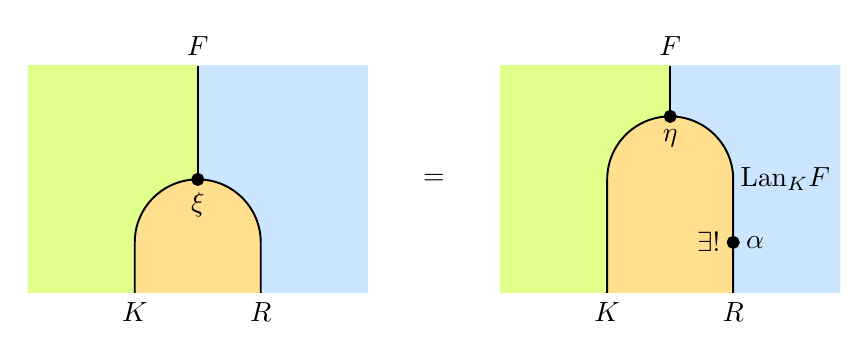
\begin{tikzpicture}[x=0.8cm,y=0.8cm, line width=0.7pt, hollow/.style={
                circle,
                fill=white,
                draw,
                outer sep=0pt,
                inner sep=1.5pt,
                line width=0.7pt
              }]
            % Define colors
            \definecolor{leftcolor}{RGB}{224, 255, 139}
            \definecolor{midcolor}{RGB}{255, 222, 142}
            \definecolor{rightcolor}{RGB}{204, 229, 255}
    
        \node at (3.75, 1.8) {$=$};
    
        \begin{scope}
            \begin{scope} 
                \clip (-2.7,0) rectangle (2.7, 3.6);     
                \fill[fill=leftcolor] (-3,0) rectangle (0, 4);  
                \fill[fill=rightcolor] (0,0) rectangle (3, 4);  
                \draw[fill=midcolor, rounded corners=0.8cm, line width=0.7pt] (-1, -3) rectangle (1, 1.8);
            \end{scope}
            \draw (0, 3.6) -- (0, 1.8);
            \filldraw [black] (0,1.8) circle (2pt) node[below=1pt] {$\xi$};
            \node[below] at (-1, 0) {$K$};
            \node[below] at (1, 0) {$R$};
            \node[above] at (0, 3.6) {$F$};
        \end{scope}
    
        \begin{scope}[shift={(7.5,0)}]
            \begin{scope} 
                \clip (-2.7,0) rectangle (2.7, 3.6);     
                \fill[fill=leftcolor] (-3,0) rectangle (0, 4);  
                \fill[fill=rightcolor] (0,0) rectangle (3, 4);  
                \draw[fill=midcolor, rounded corners=0.8cm, line width=0.7pt] (-1, -2) rectangle (1, 2.8);
            \end{scope}
            \draw (0, 3.6) -- (0,2.8);
            \filldraw [black] (1,0.8) circle (2pt) node[right=1pt] {$\alpha$} node[left=1pt] {$\exists!$};
       
            \node[below] at (-1, 0) {$K$};
            \node[right=-1pt] at (1, 1.8) {$\mathrm{Lan}_KF$};
    
            \node[below] at (1, 0) {$R$};
            \filldraw [black] (0, 2.8) circle (2pt) node[below=1pt] {$\eta$};
        
           
            \node[above] at (0, 3.6) {$F$};
        \end{scope}
    
        
        \end{tikzpicture}
    \]
    A \textbf{right Kan extension} of $K$ along $F$ is a pair $\left(\mathrm{Ran}_KF,\varepsilon\right)$ consisting of 
    \begin{itemize}
        \item a functor $\mathrm{Ran}_KF:\mathsf{D}\to\mathsf{E}$,
        \item a natural transformation $\varepsilon: \left(\mathrm{Ran}_KF\right)\circ K\Rightarrow F$
    \end{itemize}
    \begin{center}
        \begin{tikzcd}[ampersand replacement=\&, column sep=3em] 
            % drawing 0- and 1-celss 
            \mathsf{C} \arrow[dr, "K"'{name=F}] 
            \arrow[rr, "F", ""{name=H, below}] \&\& \mathsf{E} \\ 
            \& |[alias=D]| \mathsf{D} \arrow[ur, swap,
            "\mathrm{Ran}_{K}F"] 
            % % drawing 2-cells
            \arrow[Rightarrow, from=D, to=H, "\varepsilon"'] 
        \end{tikzcd}
    \end{center}
    such that for any pair $\left(L,\theta\right)$ consisting of
    \begin{itemize}
        \item a functor $L:\mathsf{D}\to\mathsf{E}$,
        \item a natural transformation $\theta:L\circ K\Rightarrow F$,
    \end{itemize}
    there exists a unique natural transformation $\beta: L\Rightarrow \mathrm{Ran}_KF$ such that
    \[
    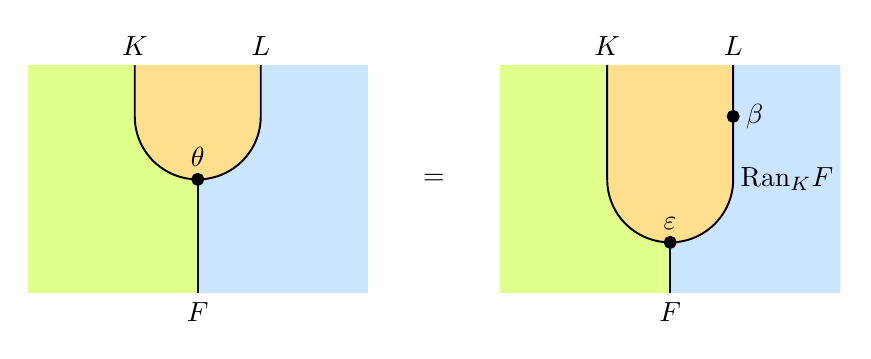
\begin{tikzpicture}[x=0.8cm,y=0.8cm, line width=0.7pt, hollow/.style={
            circle,
            fill=white,
            draw,
            outer sep=0pt,
            inner sep=1.5pt,
            line width=0.7pt
          }]
        % Define colors
        \definecolor{leftcolor}{RGB}{224, 255, 139}
        \definecolor{midcolor}{RGB}{255, 222, 142}
        \definecolor{rightcolor}{RGB}{204, 229, 255}

    \node at (3.75, 1.8) {$=$};

    \begin{scope}
        \begin{scope} 
            \clip (-2.7,0) rectangle (2.7, 3.6);     
            \fill[fill=leftcolor] (-3,0) rectangle (0, 4);  
            \fill[fill=rightcolor] (0,0) rectangle (3, 4);  
            \draw[fill=midcolor, rounded corners=0.8cm, line width=0.7pt] (-1, 6.6) rectangle (1, 1.8);
        \end{scope}
        \draw (0, 0) -- (0, 1.8);
        \filldraw [black] (0,1.8) circle (2pt) node[above=1pt] {$\theta$};
        \node[above] at (-1, 3.6) {$K$};
        \node[above] at (1, 3.6) {$L$};
        \node[below] at (0, 0) {$F$};
    \end{scope}

    \begin{scope}[shift={(7.5,0)}]
        \begin{scope} 
            \clip (-2.7,0) rectangle (2.7, 3.6);     
            \fill[fill=leftcolor] (-3,0) rectangle (0, 4);  
            \fill[fill=rightcolor] (0,0) rectangle (3, 4);  
            \draw[fill=midcolor, rounded corners=0.8cm, line width=0.7pt] (-1, 5.6) rectangle (1, 0.8);
        \end{scope}
        \draw (0, 0) -- (0,0.8);
        \filldraw [black] (1,2.8) circle (2pt) node[right=1pt] {$\beta$};
   
        \node[above] at (-1, 3.6) {$K$};
        \node[right=-1pt] at (1, 1.8) {$\mathrm{Ran}_KF$};

        \node[above] at (1, 3.6) {$L$};
        \filldraw [black] (0, 0.8) circle (2pt) node[above=1pt] {$\varepsilon$};
    
       
        \node[below] at (0, 0) {$F$};
    \end{scope}

    
    \end{tikzpicture}
\]


\end{definition}


\section{Monoidal Category}
\begin{definition}{Monoidal Category}{}
    A monoidal category is a category $\mathsf{V}$ equipped with
    \begin{enumerate}[(i)]
        \item Tensor product: a functor $\otimes:\mathsf{V}\times\mathsf{V}\to\mathsf{V}$.
        \[
            \begin{tikzcd}[ampersand replacement=\&]
                \mathsf{V}\times \mathsf{V}\&[-25pt]\&[+10pt]\&[-30pt] \mathsf{V}\&[-30pt]\&[-30pt] \\ [-15pt] 
                (X_1,Y_1)  \arrow[dd, "f\times g"{name=L, left}] 
                \&[-25pt] \& [+10pt] 
                \& [-30pt]X_1\otimes Y_1\arrow[dd, "f\otimes g"{name=R}] \\ [-10pt] 
                \&  \phantom{.}\arrow[r, "\otimes", squigarrow]\&\phantom{.}  \&   \\[-10pt] 
                (X_2,Y_2)  \& \& \& X_2\otimes Y_2
            \end{tikzcd}
            \]
        \item Associator: a natural isomorphism $a$
        \[
            \begin{tikzcd}[ampersand replacement=\&]
                \mathsf{V}\times\mathsf{V}\times\mathsf{V} \arrow[r, "(-\otimes-)\otimes-"{name=A, above}, bend left] \arrow[r, "-\otimes(-\otimes-)"'{name=B, below}, bend right] \&[+30pt] \mathsf{V}
                \arrow[Rightarrow, shorten <=5.5pt, shorten >=5.5pt, from=A.south-|B, to=B, "a", "\sim\hspace{1pt}"']
            \end{tikzcd}
        \]
        \item Unit object: an object $1\in \mathrm{Ob}(\mathsf{V})$ 
        \item An isomorphism in $\mathsf{V}$: $\iota:1\otimes 1\to 1$
    \end{enumerate}
    such that the following two condition holds
    \begin{enumerate}[(i)]
        \item The pentagon axiom: the following diagram commutes
    \[
        \begin{tikzcd}[ampersand replacement=\&, column sep=small]
            \& [-50pt]                  \&[-25pt]    ((A\otimes B)\otimes C)\otimes D \arrow[lld, "{a_{(A,B,C)}\otimes \mathrm{id}_D}"'] \arrow[rrd, "{a_{(A\otimes B,C,D)}}"] \& [-25pt]                  \&   [-50pt]                                                                      \\[+20pt]
(A\otimes( B\otimes C))\otimes D \arrow[rd, "{a_{(A,B\otimes C,D)}}"'] \&                                                                                    \&    \&       \& (A\otimes B)\otimes (C\otimes D) \arrow[ld, "{a_{(A, B, C\otimes D)}}"] \\[+35pt]
            \& A\otimes( (B\otimes C)\otimes D) \arrow[rr, "{\mathrm{id}_A\otimes a_{(B,C,D)}}"'] \&    \& A\otimes( B\otimes (C\otimes D)) \&                                                                        
\end{tikzcd}
    \]
    \item Unit axiom: the functors $1\otimes -:\mathsf{V}\to\mathsf{V}$ and $-\otimes 1:\mathsf{V}\to\mathsf{V}$ are category equivalences.
    \end{enumerate}
\end{definition}


A strict monoidal category is one for which the natural isomorphisms $a$, $\lambda$ and $\rho$ are identities. Every monoidal category is monoidally equivalent to a strict monoidal category.

\begin{definition}{Cartesian/Cocartesian Monoidal Category}{}
    \begin{itemize}[leftmargin=8pt]
        \item A \textbf{cartesian monoidal category} is a monoidal category with finite products endowed with a where the tensor product is the categorical product and the unit object is the terminal object. If a category has all finite products, then we say it is \textbf{cartesian monoidal}. 
        \item A \textbf{cocartesian monoidal category} is a monoidal category where the tensor product is the categorical coproduct and the unit object is the initial object. If a category has all finite coproducts, then we say it is \textbf{cocartesian monoidal}.
    \end{itemize}
\end{definition}


\begin{example}{Category of Endofunctors is a Monoidal Category}{}
    Let $\mathsf{C}$ be a category. The \textbf{category of endofunctors} $\left[\mathsf{C},\mathsf{C}\right]$ is a monoidal category with the following structure
    \begin{enumerate}[(i)]
        \item Tensor product: composition of functors.
        \item Associator: the natural isomorphism $a$ is the identity.
        \item Unit object: the identity functor $\mathrm{id}_{\mathsf{C}}$.
        \item Unit isomorphism: the natural isomorphism $\iota$ is the identity.
    \end{enumerate}
\end{example}


\begin{definition}{Braided Monoidal Category}{}
    A \textbf{braided monoidal category} is a monoidal category $\mathsf{V}$ equipped with an isomorphism natural in $X,Y\in \mathrm{Ob}(\mathsf{V})$
    \[
        B_{X,Y} : X \otimes Y \to Y \otimes X
    \]
    called the \textbf{braiding} such that the following two conditions hold:
    \begin{enumerate}[(i)]
        \item The hexagon axiom: the following diagram commutes
        \[
            \begin{tikzcd}[ampersand replacement=\&, column sep=small]
                \&[-50pt] (X\otimes Y)\otimes Z\arrow[rr, "{B_{X\otimes Y,Z}}"]\&[+45pt]  \&[-25pt] Z\otimes (X\otimes Y) \arrow[rd, "{a_{Z,X,Y}^{-1}}"] \&[-50pt] \\[+20pt]
                X\otimes (Y\otimes Z)\arrow[ru, "{a_{X,Y,Z}^{-1}}"] \arrow[rd, "{\mathrm{id}_X\otimes B_{Y,Z}}"'] \& \& \& \& (Z\otimes X)\otimes Y \\[+35pt]
                \& X\otimes (Z\otimes Y) \arrow[rr, "{a_{X,Z,Y}^{-1}}"'] \& \& (X\otimes Z)\otimes Y\arrow[ru, "{B_{X,Z}\otimes\mathrm{id}_Y}"']  \& 
            \end{tikzcd}
        \]
    \end{enumerate}
\end{definition}


\begin{definition}{Symmetric Monoidal Category}{}
    A \textbf{symmetric monoidal category} is a braided monoidal category $\mathsf{V}$ satisfying the following condition:
    \[
        B_{Y,X}\circ B_{X,Y}=\mathrm{id}_{X\otimes Y}.
    \]
\end{definition}

\section{Enriched Category}
\begin{definition}{Enriched Category}{enriched_category}
    Let $\mathsf{V}$ be a monoidal category. An \textbf{$\mathsf{V}$-enriched category} $\mathsf{C}$ consists of
    \begin{enumerate}[(i)]
        \item Object set: a set of objects $\mathrm{Ob}(\mathsf{C})$.
        \item $\mathrm{Hom}$-object: for each pair of objects $A,B\in \mathrm{Ob}(\mathsf{C})$, an object $\mathrm{Hom}_{\mathsf{C}}(A,B)\in \mathrm{Ob}(\mathsf{V})$.
        \item Composition: for each triple of objects $A,B,C\in \mathrm{Ob}(\mathsf{C})$, a morphism in $\mathsf{V}$
        \[
            \circ:\mathrm{Hom}_{\mathsf{C}}(B,C)\otimes \mathrm{Hom}_{\mathsf{C}}(A,B)\longrightarrow \mathrm{Hom}_{\mathsf{C}}(A,C)
        \]
        \item Identity: for each object $A\in \mathrm{Ob}(\mathsf{C})$, a morphism ${\mathcal{I}d}_A:1 \to \mathrm{Hom}_{\mathsf{C}}(A,A)$ in $\mathsf{V}$.
    \end{enumerate}
    such that the following conditions hold
    \begin{enumerate}[(i)]
        \item For each quadruple of objects $A,B,C,D\in \mathrm{Ob}(\mathsf{C})$, the following diagram in $\mathsf{V}$ commutes
        \[
            \begin{tikzcd}[ampersand replacement=\&, column sep=small]
                    \&[-130pt] {\left(\mathrm{Hom}(C,D)\otimes \mathrm{Hom}(B,C)\right)\otimes \mathrm{Hom}(A,B) } \arrow[ld, "\circ\;\otimes \,\mathrm{id}_{\mathrm{Hom}(A,B)}"'] \arrow[rr, "\cong"] \&  [-30pt]   \&  [-30pt]{\mathrm{Hom}(C,D)\otimes \left(\mathrm{Hom}(B,C)\otimes \mathrm{Hom}(A,B)\right) } \arrow[rd, "\mathrm{id}_{\mathrm{Hom}(C,D)}\,\otimes\;\circ "] \&  [-130pt]  \\[+35pt]
{\mathrm{Hom}(B,D)\otimes \mathrm{Hom}(A,B) } \arrow[rrd, "\circ"'] \&                                                                                                                                    \&                                               \&                                                                                                               \& {\mathrm{Hom}(C,D)\otimes \mathrm{Hom}(A,C) } \arrow[lld, "\circ"] \\[+20pt]
                    \&                                                                                                                                    \& {\mathrm{Hom}(A,D)} \&                                                                                                               \&                                                                   
\end{tikzcd}
    \]
    \item For each pair of objects $A,B\in \mathrm{Ob}(\mathsf{C})$, the following diagrams in $\mathsf{V}$ commute
    \[
    \begin{tikzcd}[ampersand replacement=\&, column sep=small]
        {1\otimes \mathrm{Hom}_{\mathsf{C}}(A,B)} \arrow[rr, "{{\mathcal{I}d}_B\otimes\,\mathrm{id}_{\mathrm{Hom}_{\mathsf{C}}(A,B)}}"] \arrow[rd, "\cong"'] \&                     \& {\mathrm{Hom}_{\mathsf{C}}(B,B)\otimes \mathrm{Hom}_{\mathsf{C}}(A,B)} \arrow[ld, "\circ"] \\[+10pt]
        \& {\mathrm{Hom}_{\mathsf{C}}(A,B)} \&   
\end{tikzcd}
    \]
    \[
        \begin{tikzcd}[ampersand replacement=\&, column sep=small]
            {\mathrm{Hom}_{\mathsf{C}}(A,B)\otimes 1} \arrow[rr, "\mathrm{id}_{\mathrm{Hom}_{\mathsf{C}}(A,B)}\otimes\,{\mathcal{I}d}_A "] \arrow[rd, "\cong"'] \&                     \& {\mathrm{Hom}_{\mathsf{C}}(A,B)\otimes \mathrm{Hom}_{\mathsf{C}}(A,A)} \arrow[ld, "\circ"] \\[+10pt]
            \& {\mathrm{Hom}_{\mathsf{C}}(A,B)} \&
    \end{tikzcd}
        \]
    \end{enumerate}
\end{definition}


\begin{definition}{Enriched Functor}{enriched_functor}
    Let $\mathsf{V}$ be a monoidal category and $\mathsf{C}$ and $\mathsf{D}$ be $\mathsf{V}$-enriched categories. An \textbf{$\mathsf{V}$-enriched functor} $F:\mathsf{C}\to\mathsf{D}$ consists of
    \begin{enumerate}[(i)]
        \item Object map: a map $F^{\mathrm{Ob}}:\mathrm{Ob}(\mathsf{C})\to \mathrm{Ob}(\mathsf{D})$,
        \item $\mathrm{Hom}$-object morphisms: for each pair of objects $A,B\in \mathrm{Ob}(\mathsf{C})$, a morphism $F^{\mathrm{Mor}}_{A,B}:\mathrm{Hom}_{\mathsf{C}}(A,B)\to \mathrm{Hom}_{\mathsf{D}}(F(A),F(B))$ in $\mathsf{V}$, such that for any triple of objects $A,B,C\in \mathrm{Ob}(\mathsf{C})$, the following diagram in $\mathsf{V}$ commutes
        \[
            \begin{tikzcd}[ampersand replacement=\&, column sep=small]
                {\mathrm{Hom}\left(Y,Z\right)\otimes \mathrm{Hom}\left(X,Y\right)} \arrow[rr, "\circ"] \arrow[d, "{F^{\mathrm{Mor}}_{Y,Z}\otimes F^{\mathrm{Mor}}_{X,Y}}"'] \& \& {\mathrm{Hom}\left(X,Z\right)} \arrow[d, "{F^{\mathrm{Mor}}_{X,Z}}"] \\[+15pt]
                {\mathrm{Hom}\left(FY,FZ\right)\otimes \mathrm{Hom}\left(FX,FY\right)} \arrow[rr, "\circ"'] \& \& {\mathrm{Hom}\left(FX,FZ\right)} \\
                {\mathrm{Hom}(X,X)} \arrow[rr, "{F^{\mathrm{Mor}}_{X, X}}"] \& \& {\mathrm{Hom}(FX,FX)} \\[+15pt]
                \& |[xshift=-2em,overlay]| 1 \arrow[ur] \arrow[ul] \&
            \end{tikzcd}
        \]
    \end{enumerate}
\end{definition}


\section{2-Category}

\begin{definition}{Strict 2-Category}{}
    Let $\mathsf{Cat}$ be the Cartesian monoidal category consisting of all small categories. A \textbf{strict 2-category} is a $\mathsf{Cat}$-enriched category. We define the following sets
    \begin{itemize}
        \item 0-morphism set: $\mathrm{Ob}(\mathsf{C})$
        \item 1-morphism set: $\mathrm{Hom}_{\mathsf{C}}(X,Y)$ for any $X,Y\in \mathrm{Ob}(\mathsf{C})$
        \item 2-morphism set: $\mathrm{Hom}_{\mathsf{C}}(f,g)$ for any $X,Y\in \mathrm{Ob}(\mathsf{C})$ and $f,g\in \mathrm{Hom}_{\mathsf{C}}(X,Y)$
    \end{itemize}

    For any $X,Y,Z\in\mathrm{Ob}(\mathsf{C})$, we have the following composition bifunctor
    \begin{align*}
        \begin{tikzcd}[ampersand replacement=\&]
            \mathrm{Hom}_{\mathsf{C}}(Y,Z)\times \mathrm{Hom}_{\mathsf{C}}(X,Y)\&[-25pt]\&[+10pt]\&[-30pt] \mathrm{Hom}_{\mathsf{C}}(X,Z)\&[-30pt]\&[-30pt] \\ [-15pt] 
            (f',f)  \arrow[dd, "{(\theta', \theta)}"{name=L, left},Rightarrow] 
            \&[-25pt] \& [+10pt] 
            \& [-30pt]f'\circ f\arrow[dd, "\theta'\circ \theta"{name=R},Rightarrow] \\ [-10pt] 
            \&  \phantom{.}\arrow[r, "\Theta", squigarrow]\&\phantom{.}  \&   \\[-10pt] 
            (g',g)  \& \& \& g'\circ g
        \end{tikzcd}
    \end{align*}
    which are called the horizontal composition of 2-morphisms. The functoriality of $\Theta$ means that given any vertical composition of 2-morphisms
    \[
        \begin{tikzcd}[ampersand replacement=\&]
            { (f',f)} \arrow[d, "{(\theta', \theta)}"', Rightarrow] \\
            { (g',g)} \arrow[d, "{(\psi', \psi)}"', Rightarrow]     \\
            { (h',h)}                                              
        \end{tikzcd}
    \]
    we have the following equality
    \begin{align*}
        \Theta\left(\left(\psi'\circ\theta'\right),\left(\psi\circ\theta\right)\right)=\left(\psi'\circ\theta'\right)\circ\left(\psi\circ\theta\right)=\Theta\left(\psi',\psi\right)\circ\Theta\left(\theta',\theta\right)=\left(\psi'\circ\psi\right)\circ\left(\theta'\circ\theta\right)
    \end{align*}
    which is called the \textbf{interchange law}.
\end{definition}


\begin{example}{$\mathsf{Cat}$ as 2-category}{}
    The category $\mathsf{Cat}$ is a strict 2-category with the following structure
    \begin{itemize}
        \item 0-morphism set: $\mathrm{Ob}(\mathsf{Cat})$
        \item 1-morphism set: $\mathrm{Hom}_{\mathsf{Cat}}(\mathsf{C},\mathsf{D}):=[\mathsf{C},\mathsf{D}]$ for any $\mathsf{C},\mathsf{D}\in \mathrm{Ob}(\mathsf{Cat})$
        \item 2-morphism set: $\mathrm{Hom}_{\mathsf{Cat}}(F,G):=\mathrm{Hom}_{[\mathsf{C},\mathsf{D}]}\left(F,G\right)$ for any $\mathsf{C},\mathsf{D}\in \mathrm{Ob}(\mathsf{Cat})$ and $F,G\in [\mathsf{C},\mathsf{D}]$
    \end{itemize}
\end{example}

\section{Internalization}
Traditional Bourbaki-style mathematical structures are formulated within set theory, or put differently, within the ambient category $\mathsf{Set}$. The concept of \textbf{Internalization} entails reformulating these mathematical structures in a broader ambient category $\mathsf{C}$, which typically need some extra structures to express the correponding mathematics. The extra structure required on an ambient category $\mathsf{C}$ is referred to as a \textbf{doctrine} for internalization.

\subsection{Monoid Object}
Monoids can be internalized in the doctrine of monoidal categories.

\begin{example}{Monoid Objects in Monoidal Categories}{}
    Monoid objects internal to Cartesian monoidal categories
    \begin{itemize}
        \item $\mathsf{Set}$: traditional monoid.
        \item $\mathsf{Cat}$: (small) strict monoidal category.
        \item $\mathsf{Top}$: topological monoid.
        \item $\mathsf{Mon}$: commutative monoid.
    \end{itemize}
    Monoid objects internal to general monoidal categories
    \begin{itemize}
        \item $(R\text{-}\mathsf{Mod},\otimes_{R}, R)$ for $R\in \mathrm{Ob}(\mathsf{CRing})$: associative $R$-algebra.
        \item $(\mathsf{Ab},\otimes_{\mathbb{Z}}, \mathbb{Z})$: ring.
        \item $\left(\mathsf{Ch}\left(R\text{-}\mathsf{Mod}\right),\otimes_{R}, (R)_{n\in\mathbb{Z}}\right)$ for $R\in \mathrm{Ob}(\mathsf{CRing})$:  differential graded $R$-algebra.
        \item $\left([\mathsf{C},\mathsf{C}], \circ, \mathrm{id}_{\mathsf{C}}\right)$ for $\mathsf{C}\in \mathrm{Ob}(\mathsf{Cat})$: monad on $\mathsf{C}$.
    \end{itemize}
\end{example}

Commutative monoids can be internalized in the doctrine of symmetric monoidal categories.


\subsection{Internal Category}

\begin{definition}{Internal Category}{}
    Let $\mathsf{C}$ be a category with pullbacks. A \textbf{category internal to $\mathsf{C}$} consists of
    \begin{enumerate}[(i)]
        \item Object of 0-morphisms: an object $C_0\in \mathrm{Ob}(\mathsf{C})$.
        \item Object of 1-morphisms: an object $C_1\in \mathrm{Ob}(\mathsf{C})$.
        \item Source and target morphisms: two morphisms $s,t:C_1\to C_0$.
        \item Identity assignment: a morphism $e:C_0\to C_1$.
        \item Composition: a morphism $c:C_1\times_{C_0}C_1\to C_1$.
    \end{enumerate}
    such that the following diagrams commute
    \begin{enumerate}[(i)]
        \item Source and target of identity morphisms
        \[
            \begin{tikzcd}[ampersand replacement=\&]
                \& C_0\arrow[rd, "\mathrm{id}_{C_0}"]  \arrow[ld, "\mathrm{id}_{C_0}"']\arrow[d, "e"] \&   \\
                C_0  \& C_1  \arrow[l, "s"] \arrow[r, "t"']    \&   C_0
            \end{tikzcd}
        \]
        \item Source and target of composition
        \[
            \begin{tikzcd}[ampersand replacement=\&]
                C_1\arrow[d, "s"'] \&C_1\times_{C_0}C_1 \arrow[d, "c"]\arrow[l, "\pi_1"']\arrow[r, "\pi_2"] \& C_1 \arrow[d, "t"] \\
                C_0\&C_1 \arrow[l, "s"]\arrow[r, "t"'] \& C_0                  
            \end{tikzcd}
        \]
        \item Associativity of composition 
        \item Left and right unit laws       
    \end{enumerate}
\end{definition}


\begin{definition}{Double Category}{}
    A \textbf{double category} $\mathsf{D}$ is a category internal to $\mathsf{Cat}$.
\end{definition}


\chapter{Homological Algebra}
\section{Abelian Category}

\subsection{$\mathsf{Ab}$-enriched Category}
We will refer to \hyperref[th:enriched_functor]{$\mathsf{Ab}$-enriched functors} as \textbf{additive functors}. Some literature refers to $\mathsf{Ab}$-categories as preadditive categories. We will not use this term in this note. 

\begin{definition}{Biproduct}{biproduct}
    Let $\mathsf{C}$ be an $\mathsf{Ab}$-category and $X_1$, $X_2$ be objects in $\mathsf{C}$. A \textbf{biproduct} of $X_1$ and $X_2$ is a diagram
    \[
    \begin{tikzcd}[ampersand replacement=\&]
            X_1 \arrow[r, "i_1", shift left] \& X_1\oplus X_2 \arrow[l, "p_1", shift left] \arrow[r, "p_2"', shift right] \& X_2 \arrow[l, "i_2"', shift right]
    \end{tikzcd}
    \]
    such that
    \begin{itemize}
        \item $p_1\circ i_1=\mathrm{id}_{X_1}$, $p_2\circ i_2=\mathrm{id}_{X_2}$.
        \item $i_1\circ p_1+ i_2\circ p_2=\mathrm{id}_{X_1\oplus X_2}$.
    \end{itemize}
    Empty biproduct is defined to be the zero object.
\end{definition}


\begin{proposition}{Equivalent Conditions of Existance of Biproduct}{}
    Let $\mathsf{C}$ be an $\mathsf{Ab}$-category and $X_1$, $X_2$ be objects in $\mathsf{C}$. Then the following are equivalent
    \begin{enumerate}[(i)]
        \item Product $X_1\times X_2$ exists.
        \item Coproduct $X_1\amalg X_2$ exists.
        \item Biproduct $X_1\oplus X_2$ exists.
    \end{enumerate}
\end{proposition}

\begin{proposition}{Equivalent Conditions of Existance of Zero Object}{}
    Let $\mathsf{C}$ be an $\mathsf{Ab}$-category. Then the following are equivalent
    \begin{enumerate}[(i)]
        \item Initial object (empty product) exists.
        \item Terminal object (empty coproduct) exists.
        \item Zero object (empty biproduct) exists.
    \end{enumerate}
\end{proposition}

\begin{proposition}{$\mathsf{Ab}$-enriched Functors Preserve Biproducts}{}
    $\mathsf{Ab}$-enriched functors preserve finite biproducts.
\end{proposition}


\begin{definition}{Kernel and Cokernel}{}
    Suppose $\mathsf{C}$ is a category with zero object and $f:X\to Y$ is a morphism in $\mathsf{C}$. The \textbf{kernel} of $f$ is the equalizer of $f$ and the zero morphism, which is denoted by $\ker f$. The universal property of kernel is given by the following diagram
    \[
    \begin{tikzcd}[ampersand replacement=\&]
        \& M \arrow[d, "g"] \arrow[rd, "0"] \arrow[ld, "\exists!\widetilde{g}"', dashed] \&   \\
        \ker f \arrow[r] \& X \arrow[r, "f"']                                                             \& Y
    \end{tikzcd}
    \]
    The \textbf{cokernel} of $f$ is the coequalizer of $f$ and the zero morphism, which is denoted by $\operatorname{coker}f$. The universal property of cokernel is given by the following diagram
    \[
    \begin{tikzcd}[ampersand replacement=\&]
        \& M                           \&                                                                     \\
        X \arrow[r, "f"'] \arrow[ru, "0"] \& Y \arrow[u, "g"'] \arrow[r] \& \operatorname{coker} f \arrow[lu, "\exists!\widetilde{g}"', dashed]
        \end{tikzcd}
    \]

\end{definition}


\subsection{Additive Category}
\begin{definition}{Additive Category}{}
    An $\mathsf{Ab}$-category is \textbf{additive} if it has all finite biproducts.
\end{definition}




\subsection{Abelian Category}
\begin{definition}{Abelian Category}{}
    An additive category $\mathsf{A}$ is \textbf{abelian} if 
    \begin{enumerate}[(i)]
        \item Every morphism has both a kernel and a cokernel.
        \item Every monomorphism and every epimorphism is normal. This means that every monomorphism is a kernel of some morphism, and every epimorphism is a cokernel of some morphism.
    \end{enumerate}
\end{definition}


\begin{proposition}{}{}
    If $\mathsf{A}$ is an abelian category, then $\left[\mathsf{C}, \mathsf{A}\right]$ is abelian for any small category $\mathsf{C}$.
\end{proposition}

\begin{proposition}{Exact Functors in Abelian Category}{exact_functors_in_abelian_category}
    Let $\mathsf{A}$ and $\mathsf{B}$ be abelian categories and $F:\mathsf{A}\to\mathsf{B}$ be an additive functor. Then
    \begin{enumerate}[(i)]
        \item $F$ is \hyperref[th:exact_functor]{left exact} if and only if $F$ preserves kernels, or equivalently,
        \[
        0\longrightarrow X\xlongrightarrow{f} Y\xlongrightarrow{g} Z\text{ is exact}\quad\implies\quad 0\longrightarrow F(X)\xlongrightarrow{F(f)} F(Y)\xlongrightarrow{F(g)} F(Z)\text{ is exact}.    
        \]
        \item $F$ is \hyperref[th:exact_functor]{right exact} if and only if $F$ preserves cokernels, or equivalently,
        \[
        X\xlongrightarrow{f} Y\xlongrightarrow{g} Z\longrightarrow 0\text{ is exact}\quad\implies\quad F(X)\xlongrightarrow{F(f)} F(Y)\xlongrightarrow{F(g)} F(Z)\longrightarrow 0\text{ is exact}.
        \]
        \item $F$ is \hyperref[th:exact_functor]{exact} if and only if $F$ preserves kernels and cokernels, or equivalently,
        \[
        0\longrightarrow X\xlongrightarrow{f} Y\xlongrightarrow{g} Z\longrightarrow 0\text{ is exact}\quad\implies\quad 0\longrightarrow F(X)\xlongrightarrow{F(f)} F(Y)\xlongrightarrow{F(g)} F(Z)\longrightarrow 0\text{ is exact}.
        \]
    \end{enumerate}

\end{proposition}


\begin{definition}{Cohomology Functor}{}
    Let $\mathsf{A}$ be an abelian category and 
    \[
    \begin{tikzcd}[ampersand replacement=\&]
        X \arrow[r, "f"] \& Y \arrow[r, "g"] \& Z
    \end{tikzcd}
    \]
    be an exact sequence in $\mathsf{A}$. The \textbf{cohomology functor} $\mathrm{H}:\mathsf{Ch}_{}\left(\mathsf{A}\right)\to\mathsf{Ab}$ is defined by
    \[
    \mathrm{H}(X\xlongrightarrow{f} Y\xlongrightarrow{g} Z):=\operatorname{coker}[\operatorname{im}(f) \rightarrow \operatorname{ker}(g)].
    \]
\end{definition}


    

\begin{proposition}{Exact Functor Preserve Cohomology}{exact_functor_preserve_cohomology}
    Let $F:\mathsf{A}\to\mathsf{B}$ be an exact functor between abelian categories. Suppose 
    \[
    X \xlongrightarrow{f} Y \xlongrightarrow{g} Z 
    \]
    is an exact sequence in $\mathsf{A}$. Then we have the following natural isomorphism
    \[
    F\left(\mathrm{H}\left[X \xrightarrow{f} Y\xrightarrow{g} Z\right]\right)  \cong \mathrm{H}\left[F(X) \xrightarrow{F(f)} F(Y)\xrightarrow{F(g)} F(Z)\right].
    \]
\end{proposition}

\begin{prf}
    $$
        \begin{aligned}
        F\left(\mathrm{H}\left[X \xrightarrow{f} Y\xrightarrow{g} Z\right]\right)& =F \operatorname{coker}[\operatorname{im}(f) \rightarrow \operatorname{ker}(g)] \\
        & \cong \operatorname{coker}[F \operatorname{im}(f) \rightarrow F \operatorname{ker}(g)] \\
        & \cong \operatorname{coker}[\operatorname{im}(F f) \rightarrow \operatorname{ker}(F g)]\\
        &=\mathrm{H}\left[F X \xrightarrow{F f} F Y \xrightarrow{F g} Z\right]
        \end{aligned}
$$
\end{prf}


\begin{proposition}{Hom Functors are Left Exact}{}
    Let $\mathsf{A}$ be an abelian category. Then given any $X\in \mathrm{Ob}(\mathsf{A})$, $\mathrm{Hom}_{\mathsf{A}}(X,-):\mathsf{A}\to\mathsf{Ab}$ and $\mathrm{Hom}_{\mathsf{A}}(-,X):\mathsf{A}^{\mathrm{op}}\to\mathsf{Ab}$ are left exact functors.
\end{proposition}

\begin{prf}
    To prove that $\mathrm{Hom}_{\mathsf{A}}(X,-)$ is left exact, we need to prove that it preserves kernels. Let $f:Y\to Z$ be a morphism in $\mathsf{A}$, the universal property of $\ker f$ is illustrated by the following diagram
    \[
        \begin{tikzcd}[column sep={6em, between origins}, ampersand replacement=\&]
            W \arrow[rd, "g"] \arrow[d, "\exists!h"', dashed] \&                   \&   \\[+3ex]
            \ker f \arrow[r, "\iota"']                \&Y \arrow[r, "f"', shift right=0.7ex] \arrow[r, "0", shift left=0.7ex] \& Z
        \end{tikzcd}
    \]
    It suffices to show that $\iota_*:\mathrm{Hom}_{\mathsf{A}}\left(X,\ker f \right)\hookrightarrow \mathrm{Hom}_{\mathsf{A}}\left(X,Y\right)$ satisfies the universal property of $\ker f_*$. 
    \[
        \begin{tikzcd}[column sep={10em, between origins}, ampersand replacement=\&]
            G \arrow[rd, ""] \arrow[d, "\exists!"', dashed] \&                   \&   \\[+3ex]
            \mathrm{Hom}_{\mathsf{A}}\left(X,\ker f\right) \arrow[r, "\iota_*"']                \&\mathrm{Hom}_{\mathsf{A}}\left(X,Y\right) \arrow[r, "f_*"', shift right=0.7ex] \arrow[r, "0", shift left=0.7ex] \& \mathrm{Hom}_{\mathsf{A}}\left(X,Z\right)
        \end{tikzcd}
    \]
    This reduces to checking that $\ker f_*=\iota_*\left(\mathrm{Hom}_{\mathsf{A}}\left(X,\ker f \right)\right)$. 
    
    If $\iota_*(h)\in\iota_*\left(\mathrm{Hom}_{\mathsf{A}}\left(X,\ker f \right)\right)$, then $f_*\left(\iota_*(h)\right)=f\circ \iota\circ h=0$, which means that $h\in \ker f_*$. Conversely, if $g\in \ker f_*$, then $f_*(g)=f\circ g=0$. By the universal property of $\ker f$, there exists a unique morphism $h:W\to \ker f$ such that $\iota\circ h=g$. This means that $g=\iota_*(h)\in \iota_*\left(\mathrm{Hom}_{\mathsf{A}}\left(X,\ker f \right)\right)$.

    The proof for left-exactness of $\mathrm{Hom}_{\mathsf{A}}(-,X)$ can be obtained by duality.
\end{prf}



\begin{definition}{Split Exact Sequence}{}
    Let $\mathsf{A}$ be an abelian category and 
    \[
    \begin{tikzcd}[ampersand replacement=\&]
        0 \arrow[r] \& X \arrow[r, "f"] \& Y \arrow[r, "g"] \& Z \arrow[r] \& 0
    \end{tikzcd}
    \]
    be an exact sequence in $\mathsf{A}$. The sequence is said to be \textbf{split} if there exists morphisms $r:Y\to X$ and $s:Z\to Y$ such that $Y$ is the \hyperref[th:biproduct]{biproduct} of $X$ and $Z$, which is illustrated by the following diagram
    \[
        \begin{tikzcd}[ampersand replacement=\&]
                X \arrow[r, "f", shift left] \& Y \arrow[l, "r", shift left] \arrow[r, "g"', shift right] \& Z \arrow[l, "s"', shift right]
        \end{tikzcd}
    \]
\end{definition}

\begin{proposition}{Equivalent Characterizations of Split Exact Sequence}{equivalent_split_exact_sequence}
    Let $\mathsf{A}$ be an abelian category and 
    \[
    \begin{tikzcd}[ampersand replacement=\&]
        0 \arrow[r] \& X \arrow[r, "f"] \& Y \arrow[r, "g"] \& Z \arrow[r] \& 0
    \end{tikzcd}
    \]
    be an exact sequence in $\mathsf{A}$. Then the following statements are equivalent
    \begin{enumerate}[(i)]
        \item The sequence is split.
        \item $f$ has left inverse, i.e. there exists a morphism $r:Y\to X$ such that $r\circ f=\mathrm{id}_X$.
        \begin{center}
            \begin{tikzcd}[ampersand replacement=\&, column sep={4em, between origins}, row sep={4em, between origins}]  
               0\arrow[r] \&X\arrow[d, "\mathrm{id}_X"']\arrow[r, "f"] \& Y\arrow[ld, "\exists r", dashed] \arrow[r, "g"] \& Z \arrow[r]                               \& 0\\
               \&X \&   \&   \&   
            \end{tikzcd}
        \end{center}
        \item $g$ has right inverse, i.e. there exists a morphism $s:Z\to Y$ such that $g\circ s=\mathrm{id}_Z$.
        \begin{center}
            \begin{tikzcd}[ampersand replacement=\&, column sep={4em, between origins}, row sep={4em, between origins}]
                \&  \&   \& Z \arrow[d, "\mathrm{id}_Z"] \arrow[ld, "\exists s"', dashed] \&   \\
               0\arrow[r] \&X\arrow[r, "f"'] \& Y\arrow[r, "g"'] \& Z \arrow[r]                               \& 0
            \end{tikzcd}
        \end{center}
        \item The homomorphism $f^*: \mathrm{Hom}_{\mathsf{A}}(Y,A)\to \mathrm{Hom}_{\mathsf{A}}(X,A)$ is surjective for any $A\in \mathrm{Ob}(\mathsf{A})$.
        \item The homomorphism $g_*: \mathrm{Hom}_{\mathsf{A}}(A,Y)\to \mathrm{Hom}_{\mathsf{A}}(A,Z)$ is surjective for any $A\in \mathrm{Ob}(\mathsf{A})$.
    \end{enumerate}
\end{proposition}

\begin{prf}
    (ii) $\implies$ (iv). Suppose $r:Y\to X$ is a left inverse of $f$. Given any $h\in \mathrm{Hom}_{\mathsf{A}}(X,A)$, there exists $h\circ r\in \mathrm{Hom}_{\mathsf{A}}(Y,A)$ such that $f^*(h\circ r)=h\circ r\circ f=h$, which means that $f^*$ is surjective.
    \begin{center}
        \begin{tikzcd}[ampersand replacement=\&, column sep={4em, between origins}, row sep={4em, between origins}]  
           0\arrow[r] \&X\arrow[d, "\mathrm{id}_X"']\arrow[r, "f"] \& Y \arrow[ldd, "h\circ r"]\arrow[ld, "r"', dashed] \arrow[r, "g"] \& Z \arrow[r]                               \& 0\\
           \&X \arrow[d, "h"']   \&   \&   \&   \\
           \&A \&   \&   \&
        \end{tikzcd}
    \end{center}

    (iv) $\implies$ (ii). Suppose $f^*$ is surjective. Given any $h\in \mathrm{Hom}_{\mathsf{A}}(X,A)$, there exists $h'\in \mathrm{Hom}_{\mathsf{A}}(Y,A)$ such that $f^*(h')=h$. This means that $h'\circ f=h$. Let $r:=h'$, then $r\circ f=h$.
\end{prf}



\section{Complex}

\subsection{Complex in Additive Category}
\subsubsection{Cochain Complex}
\begin{definition}{$S$-graded Object of a Category}{}
    Let $\mathsf{C}$ be a category and $S$ be a set. The category of \textbf{$S$-graded object of $\mathsf{C}$} is defined as the functor category $\left[\mathsf{Disc}(S),\mathsf{C}\right]$, denoted by $\mathsf{Gr}_{S}\left(\mathsf{C}\right)$. The explicit description of the category is given as follows
    \begin{itemize}
        \item Object: a collection of objects $\left\{X_s\right\}_{s\in S}$ in $\mathsf{C}$.
        \item Morphism: a collection of morphisms $\left\{f_s:X_s\to Y_s\right\}_{s\in S}$ in $\mathsf{C}$.
    \end{itemize}
\end{definition}


\begin{definition}{Category with Translation}{}
    A \textbf{category with translation} is a category $\mathsf{C}$ equipped with an auto-equivalence functor
    \[
    T:\mathsf{C}\longrightarrow\mathsf{C}
    \]
    called the \textbf{shift functor} or \textbf{translation functor} or suspension functor.
\end{definition}


\begin{example}{Shift Functors on $\mathbb{Z}$-graded Category}{}
    Let $\mathsf{C}$ be a category. Given $k\in \mathbb{Z}$, the \textbf{$k$-th shift functor} on $\mathsf{Gr}_{\mathbb{Z}}\left(\mathsf{C}\right)$ is an endofunctor $[k]$ defined by
    \[
        \begin{tikzcd}[ampersand replacement=\&]
            \mathsf{Gr}_{\mathbb{Z}}\left(\mathsf{C}\right)\&[-25pt]\&[+10pt]\&[-30pt]\mathsf{Gr}_{\mathbb{Z}}\left(\mathsf{C}\right)\&[-30pt]\&[-30pt] \\ [-15pt] 
            X=\left(X^i\right)  \arrow[dd, "f=\left(f^i\right)"{name=L, left}] 
            \&[-25pt] \& [+10pt] 
            \& [-30pt] X[k]=\left(X[k]^i\right)=\left(X^{k+i}\right)\arrow[dd, "{f[k]=\left(f^{k+i}\right)}"{name=R}] \\ [-10pt] 
            \&  \phantom{.}\arrow[r, "{[k]}", squigarrow]\&\phantom{.}  \&   \\[-10pt] 
            Y=\left(Y^i\right)   \& \& \& Y[k]=\left(Y[k]^i\right)=\left(Y^{k+i}\right)
        \end{tikzcd}
    \]

\end{example}


\begin{example}{Shift Functors on $\mathbb{Z}^m$-graded Category}{}
    Let $\mathsf{C}$ be a category. In a similar manner, given $k_1,\cdots,k_m\in \mathbb{Z}$, the \textbf{$(k_1,\cdots,k_m)$-th shift functor} on $\mathsf{Gr}_{\mathbb{Z}^m}\left(\mathsf{C}\right)$ is an endofunctor $[k_1,\cdots,k_m]$ defined by
    \[
        \begin{tikzcd}[ampersand replacement=\&]
            \mathsf{Gr}_{\mathbb{Z}^m}\left(\mathsf{C}\right)\&[-25pt]\&[+10pt]\&[-30pt]\mathsf{Gr}_{\mathbb{Z}^m}\left(\mathsf{C}\right)\&[-30pt]\&[-30pt] \\ [-15pt] 
            A=\left(A^{i_1,\cdots,i_m}\right)  \arrow[dd, "f=\left(f^{i_1,\cdots,i_m}\right)"{name=L, left}] 
            \&[-25pt] \& [+10pt] 
            \& [-30pt] A[k_1,\cdots,k_m]=\left(A[k_1,\cdots,k_m]^{i_1,\cdots,i_m}\right)=\left(A^{i_1+k_1,\cdots,i_m+k_m}\right)\arrow[dd, "\left(f^{i_1+k_1,\cdots,i_m+k_m}\right)"{name=R}] \\ [-10pt] 
            \&  \phantom{.}\arrow[r, "{[k_1,\cdots,k_m]}", squigarrow]\&\phantom{.}  \&   \\[-10pt] 
            B=\left(B^{i_1,\cdots,i_m}\right)   \& \& \& B[k_1,\cdots,k_m]=\left(B[k_1,\cdots,k_m]^{i_1,\cdots,i_m}\right)=\left(B^{i_1+k_1,\cdots,i_m+k_m}\right)
        \end{tikzcd}
    \]
\end{example}


\begin{lemma}{}{}
    If $\mathsf{C}$ is an additive category, then $\mathsf{Gr}_{\mathbb{Z}^m}\left(\mathsf{C}\right)=\left[\mathsf{Disc}(\mathbb{Z}^m),\mathsf{C}\right]$ is an additive category.
\end{lemma}


\begin{definition}{General Differential Object in a Category with Translation}{}
    A \textbf{general differential object} in a category $\mathsf{C}$ with translation $T$ is a pair $\left(X,d_X\right)$ consisting of an object $X$ in $\mathsf{C}$ and a morphism $d_X:X\to T(X)$ in $\mathsf{C}$.
\end{definition}


\begin{definition}{Differential Object in an Additive Category with Translation}{}
    A \textbf{differential object} in an additive category $\mathsf{C}$ with translation $T$ is a pair $\left(X,d_X\right)$ consisting of an object $X$ in $\mathsf{C}$ and a morphism $d_X:X\to T(X)$ in $\mathsf{C}$ such that $T(d_X)\circ d_X=0$.
\end{definition}


\begin{definition}{Differential $\mathbb{Z}$-Graded Object}{}
    Let $\mathsf{A}$ be an additive category. The category of \textbf{differential $\mathbb{Z}$-graded objects} of $\mathsf{A}$ consists of the following data
    \begin{itemize}
        \item Object: differential objects $\left(X,d_X\right)$ in the additive category $\mathsf{Gr}_{\mathbb{Z}}\left(\mathsf{A}\right)$ with translation $[1]$.
        \item Morphism: morphisms $f:\left(X,d_X\right)\to \left(Y,d_Y\right)$ are morphisms $f:X\to Y$ in $\mathsf{Gr}_{\mathbb{Z}}\left(\mathsf{A}\right)$ such that $f[1]\circ d_X=d_Y\circ f$.
    \end{itemize}
\end{definition}


\begin{definition}{Cochain Complex}{}
    Let $\mathsf{A}$ be an additive category. The category of \textbf{cochain complexes} of $\mathsf{A}$, denoted by $\mathsf{Ch}(\mathsf{A})$, consists of the following data
    \begin{itemize}
        \item Object: \textbf{cochain complex} of $\mathsf{A}$, which consists of a collection of objects $X^{\bullet}=\left(X^n\right)_{n\in \mathbb{Z}}$ in $\mathsf{A}$ and a collection of morphisms $d_X^{\bullet}=\left(d^n:X^n\to X^{n+1}\right)_{n\in \mathbb{Z}}$ in $\mathsf{A}$ 
        \[
            \cdots \longrightarrow X^n \xlongrightarrow{d^n_X} X^{n+1} \xlongrightarrow{d^{n+1}_X} X^{n+2} \longrightarrow \cdots
        \]
        such that $d^{n+1}_X\circ d^n_X=0$ for all $n\in \mathbb{Z}$.
        \item Morphism: a collection of morphisms $\left(f^n:X^n\to Y^{n}\right)_{n\in \mathbb{Z}}$ in $\mathsf{A}$ such that $f^{n+1}\circ d^n_X=d^n_Y\circ f^n$ for all $n\in \mathbb{Z}$
        \[
            \begin{tikzcd}[
                ampersand replacement=\&,
                column sep={6em, between origins},
                row sep={5em, between origins}
            ]
                \cdots \arrow[r] \& X^{n} \arrow[r, "d_X^n"] \arrow[d, "f^n"'] \& X^{n+1} \arrow[d, "f^{n+1}"'] \arrow[r, "d_X^{n+1}"] \& X^{n+2} \arrow[d, "f^{n+2}"] \arrow[r] \& \cdots \\
                \cdots \arrow[r] \& Y^{n} \arrow[r, "d_Y^{n}"'] \& Y^{n+1} \arrow[r, "d_Y^{n+1}"'] \& Y^{n+2} \arrow[r] \& \cdots
            \end{tikzcd}
        \]
    \end{itemize}
    $\mathsf{Ch}(\mathsf{A})$ is isomorphic to the category of differential $\mathbb{Z}$-graded objects of $\mathsf{A}$.
\end{definition}


\subsubsection{Chain Complex}
\begin{definition}{Homotopy between Morphisms of Chain Complexes}{}
    A homotopy $h$ between a pair of morphisms of chain complexes $f, g: X_{\bullet} \rightarrow Y_{\bullet}$ is a collection of morphisms $h_i: X_i \rightarrow Y_{i+1}$ such that we have
$$
f_i-g_i=d_{i+1} \circ h_i+h_{i-1} \circ d_i
$$
for all $i$. Two morphisms $f, g: X_{\bullet} \rightarrow Y_{\bullet}$ are said to be homotopic if a homotopy between $f$ and $g$ exists. 
\end{definition}

\subsection{Chain Homotopy}

\begin{definition}{Homotopy between Morphisms of Cochain Complexes}{}
    A \textbf{homotopy $h$ between a pair of morphisms of cochain complexes} $f, g: X^{\bullet} \rightarrow Y^{\bullet}$ is a collection of morphisms $h^i: X^i \rightarrow Y^{i-1}$
    \[
        \begin{tikzcd}[
            ampersand replacement=\&,
            column sep={6em, between origins},
            row sep={5em, between origins}
        ]
            \cdots \arrow[r, "d_X^{i-1}"]  \& X^{i} \arrow[r, "d_X^i"] \arrow[d, "f^i"'] \arrow[ld, "h^i"'] \& X^{i+1} \arrow[d, "f^{i+1}"'] \arrow[r, "d_X^{i+1}"] \arrow[ld, "h^{i+1}"'] \& X^{i+2} \arrow[d, "f^{i+2}"] \arrow[r, "d_X^{i+2}"] \arrow[ld, "h^{i+2}"'] \& \cdots \arrow[ld, "h^{i+3}"] \\
            \cdots \arrow[r, "d_Y^{i-1}"'] \& Y^{i} \arrow[r, "d_Y^{i}"']                                   \& Y^{i+1} \arrow[r, "d_Y^{i+1}"']                                             \& Y^{i+2} \arrow[r, "d_Y^{i+2}"']                                            \& \cdots                      
        \end{tikzcd}
    \]
         such that
$$
f^i-g^i=d^{i-1}_Y \circ h^i+h^{i+1} \circ d^i_X
$$
for all $i\in \mathbb{Z}$. Two morphisms $f, g: X^{\bullet} \rightarrow Y^{\bullet}$ are said to be \textbf{homotopic} if there exists a homotopy between $f$ and $g$. A morphism $f: X^{\bullet} \rightarrow Y^{\bullet}$ is said to be \textbf{null homotopic} if it is homotopic to the zero morphism $0: X^{\bullet} \rightarrow Y^{\bullet}$.
\end{definition}


\begin{proposition}{Additive Functor Preserves Cochain Homotopy}{}
    Let $F:\mathsf{A}\to\mathsf{B}$ be an additive functor between additive categories. Suppose $h$ is a homotopy between a pair of morphisms $f, g: X^{\bullet} \rightarrow Y^{\bullet}$ in $\mathsf{Ch}(\mathsf{A})$. Then $(F(h^i))_{i\in\mathbb{Z}}$ is a homotopy between $F(f),F(g):F\left(X^{\bullet}\right)\to F\left(Y^{\bullet} \right)$ in $\mathsf{B}$.
\end{proposition}



\begin{definition}{Homotopy Equivalence between Cochain Complexes}{}
    A morphism $f: X^{\bullet} \rightarrow Y^{\bullet}$ of cochain complexes is a \textbf{homotopy equivalence} if there exists a morphism $g: Y^{\bullet} \rightarrow X^{\bullet}$ such that $f\circ g$ and $g\circ f$ are homotopic to the identity morphisms of $X^{\bullet}$ and $Y^{\bullet}$, respectively. We say that $X^{\bullet}$ and $Y^{\bullet}$ are \textbf{homotopy equivalent} if there exists a homotopy equivalence between $X^{\bullet}$ and $Y^{\bullet}$.
\end{definition}




\subsection{Cohomology}


\begin{definition}{$n$-th Cohomology Functor}{}
    Let $\mathsf{A}$ be an abelian category. Given any $n\in \mathbb{Z}$, the \textbf{$n$-th cohomology functor} of a cochain complex $X^{\bullet}$ is defined to be the functor
    \[
    \mathrm{H}^n(X^{\bullet}):=\ker d^n/\operatorname{im}d^{n-1}.
    \]
\end{definition}


\begin{definition}{Quasi-isomorphism}{}
    A morphism $f: X^{\bullet} \rightarrow Y^{\bullet}$ of cochain complexes is a \textbf{quasi-isomorphism} if the induced morphism $\mathrm{H}^n(f):\mathrm{H}^n(X^{\bullet})\to \mathrm{H}^n(Y^{\bullet})$ is an isomorphism for all $n\in \mathbb{Z}$.
\end{definition}

\begin{lemma}{}{}
    If $f: X^{\bullet} \rightarrow Y^{\bullet}$ is null homotopic, then $\mathrm{H}^n(f)=0$ for all $n\in \mathbb{Z}$.
\end{lemma}

\begin{prf}
    Let $h$ be a homotopy between $f$ and the zero morphism. Then we have
    \[
    f^n=d^{n-1}_Y \circ h^n+h^{n+1} \circ d^n_X
    \]
    for all $n\in \mathbb{Z}$. This implies that $f^n$ induces the zero morphism on cohomology for all $n\in \mathbb{Z}$.
\end{prf}

\begin{proposition}{Homotopic Morphisms Induce the Same Morphisms on Cohomology}{}
    Let $f, g: X^{\bullet} \rightarrow Y^{\bullet}$ be homotopic morphisms of cochain complexes. Then the induced morphisms $\mathrm{H}^n(f)$ and $\mathrm{H}^n(g)$ on cohomology are the same for all $n\in \mathbb{Z}$.
\end{proposition}

\begin{prf}
    Let $h$ be a homotopy between $f$ and $g$. Then we have
    \[
    f^n-g^n=d^{n-1}_Y \circ h^n+h^{n+1} \circ d^n_X
    \]
    for all $n\in \mathbb{Z}$. This implies that $f^n$ and $g^n$ induce the same morphism on cohomology for all $n\in \mathbb{Z}$.
\end{prf}

\begin{corollary}{Homotopy Equivalences are Quasi-Isomorphisms}{}
    A homotopy equivalence of cochain complexes is a quasi-isomorphism.
\end{corollary}


\begin{definition}{Acyclic Complex}{}
    A cochain complex $X^{\bullet}$ is \textbf{acyclic} if $\mathrm{H}^n(X^{\bullet})=0$ for all $n\in \mathbb{Z}$.
\end{definition}


\begin{proposition}{}{}
    Let $\mathsf{A}$ be an abelian category and $X^{\bullet}\in\mathrm{Ob}\left(\mathsf{Ch}(\mathsf{A})\right)$ be a cochain complex. Then the following are equivalent
    \begin{enumerate}[(i)]
        \item $X^{\bullet}$ is acyclic.
        \item $X^{\bullet}$ is exact, that is, exact at each $X^n$.
        \item The zero morphism $0 \to X^{\bullet}$ is a quasi-isomorphism.
    \end{enumerate}
\end{proposition}

\section{Resolution}

\subsection{Projective and Injective Objects}
\begin{definition}{Projective Object}{}
    An object $P$ in an abelian category $\mathsf{A}$ is \textbf{projective} if for any epimorphism $f: X \rightarrow Y$ and any morphism $g: P \rightarrow Y$, there exists a morphism $h: P \rightarrow X$ such that $f \circ h = g$.
    \begin{center}
        \begin{tikzcd}[ampersand replacement=\&, column sep={5em, between origins}, row sep={5em, between origins}]
            \& P \arrow[d, "g"] \arrow[ld, "\exists h"', dashed] \&   \\
        X \arrow[r, "f"', two heads] \& Y \arrow[r]                               \& 0
        \end{tikzcd}
    \end{center}
\end{definition}


\begin{proposition}{Equivalent Characterizations of Projective Objects}{}
    Let $\mathsf{A}$ be an abelian category and $P$ be an object in $\mathsf{A}$. Then the following are equivalent
    \begin{enumerate}[(i)]
        \item $P$ is projective.
        \item $\mathrm{Hom}_{\mathsf{A}}(P,-)$ is exact.
        \item Every short exact sequence 
        \[
        \begin{tikzcd}[ampersand replacement=\&]
            0 \arrow[r] \& X \arrow[r, "f"] \& Y \arrow[r, "g"] \& P \arrow[r] \& 0
        \end{tikzcd}
        \]
        in $\mathsf{A}$ splits.
        \item $\mathop{\mathrm{Ext}}\nolimits _\mathsf{A}(P, X) = 0$ for all $X \in \mathsf{A}$.
    \end{enumerate}
\end{proposition}

\begin{prf}
    (i)$\implies$(ii). Since $\mathrm{Hom}_{\mathsf{A}}(P,-)$ is a left exact functor, it suffices to show that $\mathrm{Hom}_{\mathsf{A}}(P,-)$ preserves epimorphisms. Let $f: X \rightarrow Y$ be an epimorphism in $\mathsf{A}$. We need to show that $f_*:\mathrm{Hom}_{\mathsf{A}}(P,X)\to \mathrm{Hom}_{\mathsf{A}}(P,Y)$ is surjective. Let $g: P \rightarrow Y$ be a morphism in $\mathsf{A}$. Since $P$ is projective, there exists a morphism $h: P \rightarrow X$ such that $f_*(h)=f \circ h = g$. This means that $f_*$ is surjective.

    (i)$\implies$(iii). If $P$ is projective, then for any short exact sequence $0 \to X \xrightarrow{f} Y \xrightarrow{g} P \to 0$, there exists a morphism $h: P \to Y$ such that $h \circ g = \mathrm{id}_P$.
    \begin{center}
        \begin{tikzcd}[ampersand replacement=\&, column sep={4em, between origins}, row sep={4em, between origins}]
            \&  \&   \& P \arrow[d, "\mathrm{id}_P"] \arrow[ld, "\exists h"', dashed] \&   \\
           0\arrow[r] \&X\arrow[r, "f"'] \& Y\arrow[r, "g"', two heads] \& P \arrow[r]                               \& 0
        \end{tikzcd}
    \end{center}
    By \Cref{th:equivalent_split_exact_sequence}, this implies that the short exact sequence splits.
\end{prf}


\begin{definition}{Injective Object}{}
    An object $I$ in an abelian category $\mathsf{A}$ is \textbf{injective} if for any monomorphism $f: X \rightarrow Y$ and any morphism $g: X \rightarrow I$, there exists a morphism $h: Y \rightarrow I$ such that $h \circ f = g$.
    \begin{center}
        \begin{tikzcd}[ampersand replacement=\&, column sep={5em, between origins}, row sep={5em, between origins}]
            0 \arrow[r] \& X \arrow[r, "f", hook] \arrow[d, "g"'] \& Y \arrow[ld, "\exists h", dashed] \\
            \& I  \&                                  
        \end{tikzcd}
    \end{center}
        
\end{definition}

\begin{proposition}{Equivalent Characterizations of  Injective Objects}{}
    Let $\mathsf{A}$ be an abelian category and $I$ be an object in $\mathsf{A}$. Then the following are equivalent
    \begin{enumerate}[(i)]
        \item $I$ is injective.
        \item $\mathrm{Hom}_{\mathsf{A}}(-,I)$ is exact.
        \item Every short exact sequence 
        \[
        \begin{tikzcd}[ampersand replacement=\&]
            0 \arrow[r] \& I \arrow[r] \& X \arrow[r, "f"] \& Y \arrow[r] \& 0
        \end{tikzcd}
        \]
        in $\mathsf{A}$ splits.
        \item $\mathop{\mathrm{Ext}}\nolimits _\mathsf{A}(I, X) = 0$ for all $X \in \mathsf{A}$.
    \end{enumerate}
\end{proposition}





\chapter{Group}
\section{Basic Concepts}
\begin{definition}{Group}{}
    A \textbf{group} is a set $G$ together with a binary operation $\cdot:G\times G\to G$ such that
    \begin{enumerate}[(i)]
        \item (Associativity) $\forall x,y,z\in G$, $(x\cdot y)\cdot z=x\cdot(y\cdot z)$.
        \item (Identity) $\exists e\in G$ such that $\forall x\in G$, $e\cdot x=x\cdot e=x$.
        \item (Inverse) $\forall x\in G$, $\exists x^{-1}\in G$ such that $x\cdot x^{-1}=x^{-1}\cdot x=e$.
    \end{enumerate}
\end{definition}

Since the identity of a group is unique, we denote it by $1_G$ or simply $1$.
\begin{definition}{Opposite Group}{}
    Let $G=(G,*)$ be a group. The \textbf{opposite group} of $G$ is the group $G^{\mathrm{op}}=(G,*^{\mathrm{op}})$, where $*^{\mathrm{op}}:G\times G\to G$ is defined by $x*^{\mathrm{op}}y=y\cdot x$. If we consider $G$ as a category $\mathsf{B}G$, then we have category isomorphism
    \[
        \mathsf{B}G^{\mathrm{op}}\cong (\mathsf{B}G)^{\mathrm{op}}.
    \]
\end{definition}

\begin{proposition}{Group is Isomorphic to Its Opposite group}{}
    $G$ is isomorphic to $G^{\mathrm{op}}$ through the isomorphism $x\mapsto x^{-1}$. This is same as saying that $\mathsf{B}G$ is isomorphic to $(\mathsf{B}G)^{\mathrm{op}}$ through the functor ${}^{\mathrm{op}}$ defined in \Cref{th:functor_op}.
\end{proposition}


\begin{definition}{Subgroup}{}
    Let $G$ be a group. A subset $H$ of $G$ is called a \textbf{subgroup} of $G$ if $H$ is a group with respect to the binary operation of $G$. In this case, we write $H\le G$.
\end{definition}



\section{Group Homomorphism}
\begin{definition}{Group Homomorphism}{}
    Let $G,H$ be groups. A \textbf{group homomorphism} from $G$ to $H$ is a function $\varphi:G\to H$ such that
    \[
        \forall x,y\in G,\quad \varphi(x y)=\varphi(x)\varphi(y).
    \]
\end{definition}

\begin{definition}{Isomorphism}{}
    Let $G,H$ be groups. A group homomorphism $\varphi:G\to H$ is called an \textbf{isomorphism} if $\varphi$ is bijective. In this case, we say that $G$ and $H$ are \textbf{isomorphic} and write $G\cong H$.
\end{definition}

\begin{proposition}{Properties of Group Homomorphisms}{}
    Let $G,H$ be groups and $\varphi:G\to H$ be a group homomorphism. Then
    \begin{enumerate}[(i)]
        \item $\varphi(1_G)=1_H$.
        \item $\forall x\in G$, $\varphi(x^{-1})=\varphi(x)^{-1}$.
        \item $\forall n\in\mathbb{Z}$, $\varphi(x^n)=\varphi(x)^n$.
        \item If $K\le G$ , then $\varphi(K)\le H$.
        \item If $K\le H$, then $\varphi^{-1}(K)\le G$.
    \end{enumerate}
\end{proposition}

\begin{definition}{Kernel of Group Homomorphism}{}
    Let $\varphi:G\to H$ be a group homomorphism. The \textbf{kernel} of $\varphi$ is defined by
    \[
        \ker\varphi=\{x\in G\mid \varphi(x)=1_H\}.
    \]
\end{definition}

\begin{proposition}{Property of Kernel}{}
    Let $G$ be a group. Then
    \begin{enumerate}[(i)]
        \item Let $\varphi:G\to H$ be a group homomorphism. Then $\varphi$ is injective if and only if $\ker\varphi=\{1_G\}$.
    \end{enumerate}
\end{proposition}

\begin{definition}{Normal Subgroup}{}
    Let $G$ be a group. A subgroup $H$ of $G$ is called a \textbf{normal subgroup} if $gHg^{-1}=H$ for all $g\in G$. In this case, we write $H\lhd G$.
\end{definition}

\begin{proposition}{Equivalent Definition of Normal Subgroup}{}
    Let $G$ be a group and $H$ be a subgroup of $G$. Then the following are equivalent:
    \begin{enumerate}[(i)]
        \item $H$ is a normal subgroup of $G$.
        \item $\forall \gamma_g \in\mathrm{Inn}(G)$, $\gamma_g(H)\subseteq H$.
        \item $gHg^{-1}\subseteq H$ for all $g\in G$.
        \item $gHg^{-1}=H$ for all $g\in G$.
        \item $gH=Hg$ for all $g\in G$.
        \item $H$ is a union of conjugacy classes.
        \item $H=\ker\varphi$ for some group homomorphism $\varphi:G\to K$.
    \end{enumerate}
\end{proposition}

\begin{proposition}{Properties of Normal Subgroup}{}
    Let $G$ be a group.
    \begin{enumerate}[(i)]
        \item $\{1_G\}$ and $G$ are normal subgroups of $G$.
        \item If $H\le K\le G$ and $H\lhd G$, then $H\lhd K$.
        \item If $H\lhd_{\rm char} K\lhd G$, then $H\lhd G$.
        \item Normality is preserved under surjective homomorphisms: if $f:G \rightarrow H$ is a surjective group homomorphism and $N\lhd G$, then $f(N)\lhd H$.
        \item Normality is preserved by taking inverse images of homomorphisms: if $f:G \rightarrow H$ is a group homomorphism and $N\lhd H$, then $f^{-1}(N)\lhd G$.
        \item Normality is preserved on taking finite products: if $N_1 \lhd G_1$ and $N_2 \lhd G_2$, then $N_1 \times N_2 \lhd G_1 \times G_2$.
        \item Given two normal subgroups, $N$ and $M$, of $G$, their intersection $N \cap M$ and their product $N M=\{n m: n \in N$ and $m \in M\}$ are also normal subgroups of $G$.
    \end{enumerate}
\end{proposition}

\begin{definition}{Simple Group}{}
    A group $G$ is called \textbf{simple} if $G$ is nontrivial and the only normal subgroups of $G$ are $\{1_G\}$ and $G$.
\end{definition}

\begin{theorem}{Fundamental Theorem on Homomorphisms}{}
    Let $G,H$ be groups and $\varphi:G\to H$ be a group homomorphism. Define natural projection
    \begin{align*}
        \pi:G & \longrightarrow G/\ker\varphi \\
        g     & \longmapsto g\ker\varphi
    \end{align*}
    Then there exists a unique group homomorphism $\overline{\varphi}:G/\ker\varphi\to H$ such that the following diagram commutes
    \begin{center}
        \begin{tikzcd}[ampersand replacement=\&]
            G \arrow[r, "\varphi"] \arrow[d, "\pi"'] \& H \\[0.3cm]
            G/\ker\varphi \arrow[ru, dashed, "\exists!\,\overline{\varphi}"'] \&
        \end{tikzcd}
    \end{center}
    Moreover, $\overline{\varphi}$ is injective and we have $ G/\ker\varphi\cong \mathrm{im}\varphi$.
\end{theorem}

\begin{corollary}{First isomorphism theorem}{}
    Let $G,H$ be groups and $\varphi:G\to H$ be surjective group homomorphism. Then $G/\ker\varphi\cong H$.
\end{corollary}


\begin{proposition}{Universal Property of Quotient Group}{}
    Let $G$ be a group and $N \lhd G$ be a normal subgroup. Suppose $\pi:G\to G/N$ is the natural projection. Then $\pi$ is initial in the category of group homomorphisms $\varphi:G\to H$ such that $N\subseteq \ker\varphi$. \\
    That is, for any group $H$ and group homomorphism $\varphi:G\to H$ such that $N\subseteq \ker\varphi$, there exists a unique group homomorphism $\widetilde{\varphi}:G/N\to H$ such that the following diagram commutes
    \begin{center}
        \begin{tikzcd}[ampersand replacement=\&]
            G \arrow[r, "\varphi"] \arrow[d, "\pi"'] \& H \\[0.3cm]
            G/N \arrow[ru, dashed, "\exists !\,\widetilde{\varphi}"'] \&
        \end{tikzcd}
    \end{center}
\end{proposition}

\proof{
    Since $N\subseteq \ker\varphi$, there is a canonical projection
    \begin{align*}
        p:G/N & \longrightarrow G/\ker\varphi \\
        gN    & \longmapsto g\ker\varphi
    \end{align*}
    According to the following diagram, we can define $\widetilde{\varphi}$ by $\widetilde{\varphi}=\overline{\varphi}\circ p$.
    \begin{center}
        \begin{tikzcd}[ampersand replacement=\&]
            G \arrow[r, "\varphi"] \arrow[d, "\pi"'] \& H \\[0.4cm]
            G/N \arrow[ru, dashed, "\widetilde{\varphi}"'] \arrow[r,"p"'] \&  G/\ker\varphi \arrow[u, dashed, "\overline{\varphi}"']
        \end{tikzcd}
    \end{center}
}
\begin{theorem}{Second Isoomorphism Theorem}{}
    Let $G$ be a group and $H,K$ be subgroups of $G$. Then $HK$ is a subgroup of $G$ and $H\cap K$ is a normal subgroup of $H$. Moreover, we have
    \[
        HK/H\cong K/(H\cap K).
    \]
\end{theorem}

\section{Construction}
\subsection{Free Object}
Let $A$ be set. Define a \textbf{string} over the $A$ to be a finite sequence of elements of $A$. The \textbf{concatenation} of two strings $\overline{a_1\cdots a_n}$ and $\overline{b_1\cdots b_m}$ is a binary operation $\diamond$ defined by
\[
    \overline{a_1\cdots a_n}\diamond \overline{b_1\cdots b_m}=\overline{a_1\cdots a_nb_1\cdots b_m}.
\]
\begin{definition}{Word}{}
    Let $S$ be a set. Define $S^{-1}=\left\{s^{-1}\midv s\in S\right\}$. A \textbf{word} on $S$ is a string over $S\sqcup S^{-1}\sqcup\{1\}$. $\overline{1}$ is called an \textbf{empty word}. The \textbf{length} of a word $w$ is the number of letters in $w$.
\end{definition}

\begin{definition}{Reduced Word}{}
    Let $W(S)$ be the set of all words on $S$. Define a relation $\approx$ on $W(S)$ as follows: for any $s\in S$
    \begin{align*}
        \overline{s^{-1}s}\approx \overline{1},\quad \overline{ss^{-1}}\approx \overline{1}, \quad \overline{1s}\approx s,\quad \overline{s1}\approx \overline{1}
    \end{align*}
    Define $\sim$ to be the equivalence relation generated by $\approx$. Let $\pi:W(S)\to W(S)/\sim, w\mapsto [w]_\sim$ denote the quotient map. It is easy to see that for any $[w]_\sim\in W(S)/\sim$, there exists a unique representative element $\rho(w)\in W(S)$ which has shortest length among all representatives of $[w]_\sim$. A word $w$ is called \textbf{reduced} if $\rho(w)=w$.
\end{definition}


\begin{definition}{Free Group}{}
    Let $S$ be a set. The \textbf{free group} on $S$, denoted by $\mathrm{Free}_{\mathsf{Grp}}(S)$, together with a function $\iota:S\to \mathrm{Free}_{\mathsf{Grp}}(S)$, is defined by the following universal property: for any group $G$ and any function $f:S\to G$, there exists a unique group homomorphism $\widetilde{f}:\mathrm{Free}_{\mathsf{Grp}}(S)\to G$ such that the following diagram commutes
    \begin{center}
        \begin{tikzcd}[ampersand replacement=\&]
            \mathrm{Free}_{\mathsf{Grp}}(S)\arrow[r, dashed, "\exists !\,\widetilde{f}"]  \& G \\[0.3cm]
            S\arrow[u, "\iota"] \arrow[ru, "f"'] \&
        \end{tikzcd}
    \end{center}
    The free group $\mathrm{Free}_{\mathsf{Grp}}(S)$ can be contructed as follows: as a set it consists of all reduced words on $S$. The binary operation $\cdot$ is concatenation with reduction defined by
    \[
        w_1\cdot w_2 = \rho(w_1\diamond w_2).
    \]
    The identity element is the empty word. The inverse of a word is obtained by reversing the order of the letters and replacing each letter by its inverse.
\end{definition}


\begin{example}{Forgetful Functor $U:\mathsf{Grp}\to \mathsf{Set}$}{}
    The forgetful functor $U:\mathsf{Grp}\to \mathsf{Set}$ forgets the group structure of a group and returns the underlying set.
    \begin{enumerate}[(i)]
        \item $U$ is representable by $\left(\mathbb{Z},1\right)$. The natural isomorphism $\phi:\mathrm{Hom}_{\mathsf{Grp}}\left(\mathbb{Z},-\right)\xRightarrow{\sim} U$ is given by
              \begin{align*}
                  \phi_G:\mathrm{Hom}_{\mathsf{Grp}}\left(\mathbb{Z},G\right) & \xlongrightarrow{\sim} U(G) \\
                  f                                                           & \longmapsto f(1).
              \end{align*}
              A group homomorphism from $\mathbb{Z}$ to $G$ is uniquely determined by its action on $1$.
        \item $U$ is faithful but not full.
    \end{enumerate}
\end{example}

\begin{prf}
    \begin{enumerate}[(i)]
        \item $\phi:\mathrm{Hom}_{\mathsf{Grp}}\left(\mathbb{Z},-\right)\xRightarrow{\sim} U$ is the composition of the following natural isomorphisms
              \[
                  \mathrm{Hom}_{\mathsf{Grp}}\left(\mathbb{Z},-\right)\cong\mathrm{Hom}_{\mathsf{Grp}}(\mathrm{Free}_{\mathsf{Grp}}(\{*\}),-)\cong \mathrm{Hom}_{\mathsf{Set}}(\{*\},U(-))\cong U.
              \]
        \item $U$ is not full because not every mapping $f:\mathbb{Z}\to G$ is a group homomorphism.
    \end{enumerate}
\end{prf}


\begin{proposition}{Free-Forgetful Adjunction $\mathrm{Free}_{\mathsf{Grp}}\dashv U$}{}
    The free group functor $\mathrm{Free}_{\mathsf{Grp}}$ is left adjoint to the forgetful functor $U:\mathsf{Grp}\to \mathsf{Set}$
    $$
        \begin{tikzcd}[ampersand replacement=\&]
            \mathsf{Set} \arrow[rr, "\mathrm{Free}_{\mathsf{Grp}}", bend left] \&[-10pt]\bot\&[-10pt] \mathsf{Grp} \arrow[ll, "U", bend left]
        \end{tikzcd}
    $$
    The adjunction isomorphism is given by
    \begin{align*}
        \varphi_{S,G}:\mathrm{Hom}_{\mathsf{Grp}}(\mathrm{Free}_{\mathsf{Grp}}(S),G) & \xlongrightarrow{\sim} \mathrm{Hom}_{\mathsf{Set}}(S,U(G)) \\
        g                                                                            & \longmapsto g\circ \iota
    \end{align*}
\end{proposition}

\begin{prf}
    First we show that $\varphi_{S,G}$ is injective. Suppose $g_1,g_2:\mathrm{Free}_{\mathsf{Grp}}(S)\to G$ are two group homomorphisms such that $g_1\circ \iota=g_2\circ \iota$. By the universal property of free group, we have $g_1=g_2$. Then we show that $\varphi_{S,G}$ is surjective. Suppose $f:S\to U(G)$ is a function. By the universal property there exists a group homomorphism $\widetilde{f}:\mathrm{Free}_{\mathsf{Grp}}(S)\to G$ such that $\varphi_{S,G}(\widetilde{f})=\widetilde{f}\circ \iota=f$. Finally, we show that $\varphi_{S,G}$ is natural in $S$ and $G$. Suppose $h:S_1\to S_2$ is a function and $q:G_1\to G_2$ is a group homomorphism. Then we can check that for any $g\in \mathrm{Hom}_{\mathsf{Grp}}(\mathrm{Free}_{\mathsf{Grp}}(S_2),G_2)$,
    \begin{align*}
        \varphi_{S_1,G_1}(q\circ g\circ \iota_{S_1}) & =(q\circ g\circ \iota_{S_1})\circ \iota_{S_1} \\
                                                     & =q\circ g\circ (\iota_{S_1}\circ \iota_{S_1}) \\
                                                     & =q\circ g\circ \iota_{S_2}                    \\
                                                     & =\varphi_{S_2,G_2}(g\circ \iota_{S_2}).
    \end{align*}
\end{prf}




\subsection{Inverse Limit}
\begin{definition}{Inverse Limit in $\mathsf{Grp}$}{inverse_limit_of_groups}
    Let $\mathsf{I}$ be a \hyperref[th:filtered_category]{filtered} \hyperref[th:thin_category]{thin category} and $F:\mathsf{I}^{\mathrm{op}}\to \mathsf{Grp}$ be a functor. To unpack the information of $F$, denote $I:=\mathrm{Ob}(\mathsf{I})$, $G_i:=F(i)$ and $f_{ij}:=F(i\to j)$. An \textbf{inverse system} is a pair $\left(\left(G_i\right)_{i \in I},\left(f_{i j}\right)_{i \leq j \in I}\right)$ where $f_{i j}: G_{j} \rightarrow G_{i}$ is a group homomorphism for each $i \leq j$ such that
    \begin{enumerate}[(i)]
        \item $f_{i i}=\mathrm{id}_{G_i}$ for all $i \in I$.
        \item $f_{i k}=f_{i j} \circ f_{j k}$ for all $i \leq j \leq k$.
    \end{enumerate}
    The \textbf{inverse limit} of $\left(\left(G_i\right)_{i \in I},\left(f_{i j}\right)_{i \leq j \in I}\right)$ is the cofiltered limit $\varprojlim F$, also denoted by $\varprojlim_{i\in I}G_i$, which can be constructed as a subgroup of $\prod_{i \in I} G_{i}$ as follows
    \[
        \varprojlim_{i\in I}G_i \cong \left\{(x_i)_{i\in I}\in \prod_{i \in I} G_{i}\midv x_i=f_{ij}(x_j) \text{ for all }i\le j \in I\right\}
    \]
    equipped with natural projections $\pi_i:\varprojlim_{i\in I}G_i\to G_i$.\\

\end{definition}


\begin{example}{Inverse Limit $\varprojlim_{i\ge 1}G_i$}{}
    Let $\mathsf{I}=\left(\mathbb{Z}_{\ge 1},\le\right)$ be a filtered thin category and $F:\mathsf{I}^{\mathrm{op}}\to \mathsf{Grp}$ be a functor. To determine an inverse system, it is sufficient to specify $G_i$ and $f_{i,i+1}:G_{i+1}\to G_i$ for all $i\in \mathbb{Z}_{\ge 1}$. The inverse limit of this inverse system is denoted by $\varprojlim_{i\ge 1}G_i$, which we now write as $G$ for simplicity.\\
    $G$ can be imaged as a tree with root layer being $G_0=\{1\}$ and $i$-th layer being $G_i$. Each node in $G_i$ has a unique parent node in $G_{i-1}$, which is determined by $f_{i,i-1}$. An element in $G$ is a path starting from the root and passing through each $G_i$ exactly once along the edges of the tree. The $i$-th component $x_i$ of an element $x\in G$ includes all information of its history path from $G_0$ to $G_i$, which makes $x_1,x_2,\cdots, x_{i-1}$ redundant.
\end{example}


\section{Group Action}
\subsection{Definitions}
\begin{definition}{Symmetric Group}{}
    The \textbf{symmetric group} on a set $X$ is the group whose elements are all bijections from $X$ to $X$, with the group operation of function composition. The symmetric group on $X$ is denoted by $\mathrm{Sym}(X)$ or $\mathrm{Aut}_{\mathsf{Set}}(X)$. If $X=\{1,2,\cdots,n\}$, then we denote $\mathrm{Sym}(X)$ by $S_n$.
\end{definition}

\begin{definition}{Group Action}{}
    Let $G$ be a group and $X$ be a set. A \textbf{group action} of $G$ on $X$ is a group homomorphism
    \begin{align*}
        \sigma:G & \longrightarrow \mathrm{Aut}_{\mathsf{Set}}(X) \\
        g        & \longmapsto \sigma_g
    \end{align*}
    If $G$ acts on $X$ by $\sigma$, we say $(X,\sigma)$ is a \textbf{$G$-set}. If there is no ambiguity, we simply say $X$ is a $G$-set.
\end{definition}



\begin{proposition}{Equivalent Definition of Group Actions}{}
    Let $G$ be a group and $X$ be a set. A group action of $G$ on $X$ can be alternatively defined as a map
    \begin{align*}
        \cdot:G\times X & \longrightarrow X    \\
        (g,x)           & \longmapsto g\cdot x
    \end{align*}
    such that
    \begin{enumerate}[(i)]
        \item $\forall x\in X$, $e\cdot x=x$.
        \item $\forall g,h\in G$, $\forall x\in X$, $(gh)\cdot x=g\cdot(h\cdot x)$.
    \end{enumerate}
    The equivalence of the two definitions is given by
    \[
        \sigma_g(x)=g\cdot x.
    \]
\end{proposition}

We say $X$ is a right $G$-set if $X$ is a left $G^{\mathrm{op}}$-set.

\begin{definition}{$G$-equivariant Map}{}
    Let $G$ be a group and $(X,\sigma)$, $(Y,\sigma')$ be $G$-sets. A map $f:X\to Y$ is called \textbf{$G$-equivariant} if for all $g\in G$ and $x\in X$, we have
    \[
        f(g\cdot x)=g\cdot f(x)    .
    \]
    Equivalently, $f$ is $G$-equivariant if it is a natural transformation $f:\sigma(-)\implies \sigma'(-)$ such that for any $g\in G$, the following naturality diagram commutes
    \[
        \begin{tikzcd}[ampersand replacement=\&, column sep=1.7em, row sep=small]
            \mathsf{B}G  \& \bullet \arrow[rr, "g"]                         \&  \& \bullet                 \\
            \& X \arrow[dd, "f"'] \arrow[rr, "\sigma_g"] \&  \& X \arrow[dd, "f"] \\
            \mathsf{Set} \&                                           \&  \&                   \\
            \& Y \arrow[rr, "\sigma'_g"']                \&  \& Y
        \end{tikzcd}
    \]
\end{definition}

\begin{definition}{Category of $G$-sets}{}
    The categories of left $G$-sets, denoted by $G\text{-}\mathsf{Set}$, are defined as follows:
    \begin{itemize}
        \item Objects: $G$-sets.
        \item Morphisms: $G$-equivariant maps.
        \item Composition of morphisms is the composition of functions.
    \end{itemize}
    $G\text{-}\mathsf{Set}$ can be identified with the functor category $[\mathsf{B}G,\mathsf{Set}]$, given by the following isomorphism of categories
\begin{align*}
    G\text{-}\mathsf{Set} & \stackrel{\sim}{\longrightarrow}[\mathsf{B}G, \mathsf{Set}] \\
    (X,\sigma )               & \longmapsto \left(\bullet \rightarrow X,\;\, \sigma:G\to \mathrm{Aut}_{\mathsf{Set}}(X)\right)
\end{align*}
    
\end{definition}


\begin{example}{Trivial Group Action}{}
    Let $G$ be a group and $X$ be a set. The \textbf{trivial group action} of $G$ on $X$ is defined as $\sigma_g=\mathrm{id}_X$ for all $g\in G$.
\end{example} 


\begin{example}{Actions on $X$ Induce Actions on $2^X$}{acting_on_power_set}
    If a group $G$ acts on a set $X$, then $G$ acts on the power set $2^X$ by
    \[
        g\cdot A=\{ g\cdot x\mid x\in A\}    .
    \]
\end{example}


\begin{definition}{Product of $G$-Sets}{}
    The \textbf{product} of two $G$-sets $X$ and $Y$ is defined as the set $X\times Y$ with the $G$-action
    \[
        g\cdot (x,y)=(g\cdot x, g\cdot y)    .
    \]
    Alternatively, the product of two $G$-sets can be defined as the product of two functors, cf. \Cref{th:ev_functor_preserves_limits}.
\end{definition}

\begin{definition}{Coproduct of $G$-Sets}{}
    The \textbf{coproduct} of two $G$-sets $X$ and $Y$ is defined as the set $X\sqcup Y$ with the $G$-action
    \[
        g\cdot a=\begin{cases}
            g\cdot a & a\in X \\
            g\cdot a & a\in Y
        \end{cases}
    \]
    Alternatively, the coproduct of two $G$-sets can be defined as the coproduct of two functors, cf. \Cref{th:ev_functor_preserves_limits}.
\end{definition}

\begin{example}{$\mathrm{Aut}_\mathsf{C}(X)$ acts on $\mathrm{Hom}_\mathsf{C}(X,Y)$ and $\mathrm{Hom}_\mathsf{C}(Y,X)$}{aut_acts_on_hom}
    Let $X$ and $Y$ be objects in a category $\mathsf{C}$. Then $\mathrm{Aut}_\mathsf{C}(X)$ acts on $\mathrm{Hom}_\mathsf{C}(X,Y)$ by the composition of functors
    \[
        \begin{tikzcd}[ampersand replacement=\&, column sep=5em, row sep=3em]
            \mathsf{B}\mathrm{Aut}_\mathsf{C}(X)\arrow[r,"{(-)}^{-1}"] \&[-3em] \mathsf{B}\mathrm{Aut}_\mathsf{C}(X)^{\mathrm{op}} \arrow[r, hook] \&[-2em] \mathsf{C}^{\mathrm{op}} \arrow[r, "{\mathrm{Hom}_{\mathsf{C}}(-,Y)}"] \& \mathsf{Set}\\[-2.3em]
            \bullet \arrow[r, maps to] \arrow[d, "g"']           \& \bullet \arrow[r, maps to] \arrow[d, "g^{-1}"]                           \& X \arrow[d, "g^{-1}"] \arrow[r, maps to]                               \& {\mathrm{Hom}(X,Y)} \arrow[d, "\left(g^{-1}\right)^*"] \\
            \bullet \arrow[r, maps to]                           \& \bullet \arrow[r, maps to]                                               \& X \arrow[r, maps to]                                                   \& {\mathrm{Hom}(X,Y)}
        \end{tikzcd}
    \]
    Writing explicily, the action is given by
    \begin{align*}
        \mathrm{Aut}_\mathsf{C}(X)\times \mathrm{Hom}_\mathsf{C}(X,Y) & \longrightarrow \mathrm{Hom}_\mathsf{C}(X,Y) \\
        (g,f)                                                         & \longmapsto f\circ g^{-1}
    \end{align*}
    Similarly, $\mathrm{Aut}_\mathsf{C}(Y)$ acts on $\mathrm{Hom}_\mathsf{C}(Y,X)$ by
    \[
        \begin{tikzcd}[ampersand replacement=\&, column sep=5em, row sep=3em]
            \mathsf{B}\mathrm{Aut}_\mathsf{C}(X)\arrow[r, hook] \&[-1em] \mathsf{C} \arrow[r, "{\mathrm{Hom}_{\mathsf{C}}(Y,-)}"] \& \mathsf{Set}\\[-2.3em]
            \bullet \arrow[r, maps to] \arrow[d, "g"']           \&  X \arrow[d, "g"] \arrow[r, maps to]                               \& {\mathrm{Hom}(Y,X)} \arrow[d, "g_*"] \\
            \bullet \arrow[r, maps to]                           \& X \arrow[r, maps to]                                                   \& {\mathrm{Hom}(X,Y)}
        \end{tikzcd}
    \]
    Writing explicily, the action is given by
    \begin{align*}
        \mathrm{Aut}_\mathsf{C}(Y)\times \mathrm{Hom}_\mathsf{C}(Y,X) & \longrightarrow \mathrm{Hom}_\mathsf{C}(Y,X) \\
        (g,f)                                                         & \longmapsto g\circ f
    \end{align*}
\end{example}

\begin{example}{Actions on $X$ Induce Actions on $\mathrm{Hom}_{\mathsf{Set}}(X,Y)$}{acting_on_functions}
    If $G$ acts on $X$ through a functor $\sigma(-):\mathsf{B}G\to\mathsf{Set}$, then it also acts on $\mathrm{Hom}_{\mathsf{Set}}(X,Y)$ for any set $Y$ by the composition of functors
    \[
        \begin{tikzcd}[ampersand replacement=\&, column sep=5em, row sep=3em]
            \mathsf{B}G \arrow[r,"{(-)}^{-1}"] \&[-2em] \mathsf{B}G^{\mathrm{op}} \arrow[r, "\sigma(-)^{\mathrm{op}}"] \&[-2.2em] \mathsf{Set}^{\mathrm{op}} \arrow[r, "{\mathrm{Hom}_{\mathsf{Set}}(-,Y)}"] \& \mathsf{Set}
        \end{tikzcd}
    \]
    The left action on $\mathrm{Hom}_{\mathsf{Set}}(X,Y)$ is given explicitly as follows: for all $g\in G$, $f\in \mathrm{Hom}_{\mathsf{Set}}(X,Y)$ and $x\in X$,
    \[
        (g\cdot f)(x)=f(g^{-1}\cdot x).
    \]
    Equivalently, the right action $\star$ on $\mathrm{Hom}_{\mathsf{Set}}(X,Y)$ is given by
    \[
        (f\star g)(x)=f(g\cdot x).
    \]


\end{example}

\begin{prf}
    We can check that
    \begin{align*}
        (g_1\cdot (g_2\cdot f))(x) & =\left(g_2\cdot f\right)\left(g_1^{-1}\cdot x\right)     \\
                                   & =\left(g_2\cdot f\right)\left(g_1^{-1}\cdot x\right)     \\
                                   & =f\left(g_2^{-1}\cdot\left(g_1^{-1}\cdot x\right)\right) \\
                                   & =f\left(\left(g_2^{-1} g_1^{-1}\right)\cdot x\right)     \\
                                   & =\left(\left(g_1g_2\right)\cdot f\right)(x).
    \end{align*}
    and also check that
    \begin{align*}
        ((f\star g_1)\star g_2)(x)
         & =\left(f\star g_1\right)\left(g_2\cdot x\right) \\
         & =f\left(g_1\cdot\left(g_2\cdot x\right)\right)  \\
         & =f\left((g_1g_2)\cdot x\right)                  \\
         & =\left(f\star (g_1 g_2)\right)(x).
    \end{align*}
\end{prf}

\begin{definition}{Orbit of a Group Action}{}
    Let $G$ be a group acting on a set $X$. For $x\in X$, the \textbf{orbit} of $x$ is defined as
    \[
        G x=\{ g\cdot x\mid g\in G\}    .
    \]
\end{definition}


\begin{definition}{Orbit Space}{}
    Let $G$ be a group acting on a set $X$. The \textbf{orbit space} of $G$ acting on $X$ is defined as
    \[
        G\backslash X=\{ Gx\mid x\in X\}.
    \]
\end{definition}

If $G$ acts on $X$, then $G$ acts on $G\backslash X$ trivially by $g\cdot Gx=Gx$.
\begin{proposition}{Orbit Decomposition}{}
    Let $G$ be a group acting on a set $X$. We define a equivalence relation $\sim$ on $X$ by
    \[
        x\sim y \iff Gx=Gy.
    \]
    Then the equivalence class of $x$ is exactly $Gx$. The quotient set $X/\sim$ is exactly the orbit space $G\backslash X$.
    And we have a partition of $X$ by the orbits of $G$ acting on $X$
    \[
        X=\bigsqcup_{Gx\in G\backslash X}Gx.
    \]
\end{proposition}

\begin{prf}
    We can check that the equivalence class of $x$ is $Gx$. If $y\sim x$, then $y\in Gy=Gx$. If $y\in Gx$, then $Gy\subseteq Gx$ and $x\in Gy$. Note $x\in Gy$ implies $Gx\subseteq Gy$. We have $Gx=Gy$, i.e. $x\sim y$.
\end{prf}


If $G$ acts on $X$, then $G$ acts on $G\backslash X$ trivially.
\begin{definition}{$G$-invariant element }{}
    Let $G$ be a group acting on a set $X$. An element $x\in X$ is called \textbf{$G$-invariant} if $Gx=\{ x\}$ or equivalently $|Gx|=1$. The set of all $G$-invariant elements is denoted by $X^G$
    \[
        X^G=\{ x\in X\mid Gx=\{ x\} \} =  \{ x\in X\mid \forall g\in G, g\cdot x=x \} .
    \]
\end{definition}


\begin{definition}{Stabilizer Subgroup}{}
    Let $G$ be a group acting on a set $X$. For $x\in X$, the \textbf{stabilizer subgroup} of of $G$ with respect to $x$ is defined as
    \[
        \mathrm{Stab}_G(x)=\{ g\in G\mid g\cdot x=x\}    .
    \]
    It is easy to see that $\mathrm{Stab}_G(x)$ is a subgroup of $G$.
\end{definition}

\begin{proposition}{Properties of Stabilizer Subgroup}{properties_of_stabilizer_subgroup}
    Let $G$ be a group acting on a set $X$. For $x\in X$, the stabilizer subgroup $\mathrm{Stab}_G(x)$ has the following properties
    \begin{enumerate}[(i)]
        \item $x\in X^G\iff \mathrm{Stab}_G(x)=G$.
        \item $\ker \left(G\to \mathrm{Aut}_{\mathsf{Set}}(X)\right)=\bigcap\limits_{x\in X}\mathrm{Stab}_G(x)$.
        \item $\mathrm{Stab}_G(gx)=g\mathrm{Stab}_G(x)g^{-1}$ for any $g\in G$. Hence, $\{\mathrm{Stab}_G(x)\mid x\in X\}$ is a conjugacy class in $G$.
    \end{enumerate}
    If $X \curvearrowleft G$ is a right action, then we have $\mathrm{Stab}_G(xg)=g^{-1}\mathrm{Stab}_G(x)g$ for any $g\in G$.
\end{proposition}
\begin{proof}
    \begin{enumerate}[(i)]
        \item 
        $$
        x \in X^G \iff \forall g \in G, gx = x \iff \mathrm{Stab}_G(x) = G.
        $$
        \item 
        $$
        g \in \ker \left(G \to \mathrm{Aut}_{\mathsf{Set}}(X) \right) \iff  \forall x \in X ,\; gx = x \iff g \in \bigcap_{x \in X} \mathrm{Stab}_G(x).
        $$    
        \item  Let $h \in \mathrm{Stab}_G(gx)$, meaning $h(gx) = gx$.
        Applying $g^{-1}$ to both sides, we get $g^{-1}h(gx) = g^{-1}(gx)=x$. Thus, $g^{-1}hg \in \mathrm{Stab}_G(x)$, meaning $h \in g \mathrm{Stab}_G(x) g^{-1}$.
        Conversely, if $h \in g \mathrm{Stab}_G(x) g^{-1}$, then $h = g k g^{-1}$ for some $k \in \mathrm{Stab}_G(x)$. Therefore, $h(gx) = g(kx) = gx$, so $h \in \mathrm{Stab}_G(gx)$.
        Thus, $\mathrm{Stab}_G(gx) = g \mathrm{Stab}_G(x) g^{-1}$.
    \end{enumerate}
\end{proof}


\begin{definition}{Faithful Group Action}{}
    Let $G$ be a group acting on a set $X$. The action is called \textbf{faithful} if any of the following equivalent conditions holds
    \begin{enumerate}[(i)]
        \item $G\to \mathrm{Aut}_{\mathsf{Set}}(X)$ is injective.
        \item $\bigcap\limits_{x\in X}\mathrm{Stab}_G(x)=\{ 1_G\}$.
        \item $\forall x\in X,\;g\cdot x=x\implies g=1_G$.
    \end{enumerate}
\end{definition}


\begin{definition}{Free Group Action}{}
    Let $G$ be a group acting on a set $X$. The action is called \textbf{free} if any of the following equivalent conditions holds
    \begin{enumerate}[(i)]
        \item For all $x\in X$, $\mathrm{Stab}_G(x)=\{ 1_G\}$ .
        \item $\exists x\in X,\;g\cdot x=x\implies g=1_G$.
    \end{enumerate}
\end{definition}

It is clear that a free action is faithful, but the converse does not hold in general.

\begin{definition}{Transitive Group Action}{}
    Let $G$ be a group acting on a set $X$. The action is called \textbf{transitive} if any of the following equivalent conditions holds
    \begin{enumerate}[(i)]
        \item For any $x,y\in X$, there exists $g\in G$ such that $g\cdot x=y$.
        \item $X$ has only one orbit, i.e. $X= Gx$ for any $x\in X$.
    \end{enumerate}
    If $G$ acts transitively on $X$, then $X$ is called a \textbf{homogeneous space} for $G$.
\end{definition}

The following proposition shows that we can understand a group action on a set $X$ by studying the group action on each $G$-orbit $Gx$ separately.

\begin{proposition}{$G$ Acts on Orbit $Gx$ Transitively}{}
    Let $G$ be a group acting on a set $X$ and $x\in X$. Then $G$ acts on the orbit $Gx$ by left multiplication transitively. And we have a $G$-set isomorphism
    \[
        X\cong \bigsqcup_{Gx\in G\backslash X}Gx,
    \]
    which decomposes any $G$-set into coproduct of transitive $G$-sets.
\end{proposition}

\begin{example}{The Orbit Decomposition of Subgroup Action}{}
    Let $G$ be a group acting on a set $X$ with orbit decomposition
    \[
        X=\bigsqcup_{i \in I} G x_i
    \]
    Suppose $H$ be a subgroup of $G$ and $G$ has right coset decomposition
    \[
        G=\bigsqcup_{j \in J} Hg_j
    \]
    Then $H$ also acts on $X$ and each $G$-orbit is disjoint union of some $H$-orbits, which can written as
    \[
        Gx_i =\bigsqcup_{k \in K} H s_{ik}.
    \]
    More concretely, $Gx_i$ is the union of the cosets $H (g_jx_i)\;(j \in J)$,
    \[
        Gx_i =\bigcup_{j \in J} H g_j x_i.
    \]
    But $H (g_{j}x_i)$ may coincide with $H (g_{j'}x_i)$ for $j\ne j'$. We can duplicate $H (g_jx_i)\;(j \in J)$ by checking if there exists $h \in H$ such that $h g_j s_i=g_{j'} s_i$. Suppose $a \sim_H b$ iff $a$ and $b$ in the same $H$-orbit. Then we get
    \[
        \{s_{ik}\mid k \in K\}=\{g_j x_i \mid j \in J\}/\sim_H.
    \]
\end{example}

\begin{definition}{Regular Group Action}{}
    Let $G$ be a group acting on a set $X$. The action is called \textbf{regular} if any of the following equivalent conditions holds
    \begin{enumerate}[(i)]
        \item The action is transitive and free.
        \item For any $x,y\in X$, there exists unique $g\in G$ such that $g\cdot x=y$.
    \end{enumerate}
    If $G$ acts regularly on $X$, then $X$ is called a \textbf{principal homogeneous space} for $G$ or a $G$-\textbf{torsor}.
\end{definition}

\subsection{Coset}
\begin{example}{Left Multiplication Action}{}
    Let $G$ be a group. The \textbf{left multiplication action} of $G$ on itself is defined as
    \begin{align*}
        m^L:G & \longrightarrow \mathrm{Aut}(G) \\
        g     & \longmapsto ( x\longmapsto gx)
    \end{align*}
\end{example}

\begin{example}{Right Multiplication Action}{}
    Let $G$ be a group. The \textbf{right multiplication action} of $G$ on itself is defined as
    \begin{align*}
        m^R:G^\circ & \longrightarrow \mathrm{Aut}(G) \\
        g           & \longmapsto ( x\longmapsto xg)
    \end{align*}
\end{example}

\begin{definition}{Left Cosets}{}
    Let $G$ be a group and $H$ be a subgroup of $G$. $H^\circ$ can act on $G$ through $H^\circ\hookrightarrow G^\circ\stackrel{m^R}{\longrightarrow} \mathrm{Aut}(G)$, namely
    \begin{align*}
        H^\circ & \longrightarrow \mathrm{Aut}(G) \\
        h       & \longmapsto  (g\longmapsto gh)
    \end{align*}
    The orbit of $g$ under $H^\circ$ is called the \textbf{left coset} of $H$ containing $g$, denoted by $gH$
    \[
        gH = H^\circ g = \{ gh\mid h\in H\}.
    \]
    The set of all left cosets of $H$ is denoted by $G/H$, called the left coset space of $G$ modulo $H$. $G/H$ is the orbit space of $G$ under the right multiplication action of $H$.
\end{definition}

\begin{example}{$G$ Acts on $G/H$ Transitively}{}
    Let $G$ be a group and $H$ be a subgroup of $G$. $G$ acts on $G/H$ through
    \begin{align*}
        G & \longrightarrow \mathrm{Aut}(G/H) \\
        g & \longmapsto  (xH\longmapsto gxH)
    \end{align*}
    For any $xH,yH\in G/H$, we have $yH=gxH$ for some $g=yx^{-1}\in G$. Thus $G$ acts on $G/H$ transitively.
\end{example}

\begin{definition}{Right Cosets}{}
    Let $G$ be a group and $H$ be a subgroup of $G$. $H$ can act on $G$ through $H\hookrightarrow G\stackrel{m^L}{\longrightarrow} \mathrm{Aut}(G)$, namely
    \begin{align*}
        H & \longrightarrow \mathrm{Aut}(G) \\
        h & \longmapsto  (g\longmapsto hg)
    \end{align*}
    The orbit of $g$ under $H$ is called the \textbf{right coset} of $H$ containing $g$, denoted by $Hg$
    \[
        Hg = \{ hg\mid h\in H\},
    \]
    which matches notation of orbit. The set of all right cosets of $H$ is denoted by $H\backslash G$, called the right coset space of $G$ modulo $H$.
\end{definition}

\begin{definition}{Index of Subgroup}{}
    Let $G$ be a group and $H$ be a subgroup of $G$. The \textbf{index} of $H$ in $G$ is defined as the cardinality of $G/H$ or $H\backslash G$, denoted by $[G:H]$.
\end{definition}

\begin{theorem}{Lagrange's Theorem}{}
    Let $G$ be a finite group and $H$ be a subgroup of $G$. Then $|G|=|H|[G:H]$.
\end{theorem}


\begin{proposition}{$G$-Set Isomorphism $G/\mathrm{Stab}_G(x)\cong Gx$}{iso_stab_orbit}
    Let $G$ be a group acting on a set $X$ and $x\in X$. Then the map
    \begin{align*}
        F:G/\mathrm{Stab}_G(x)          & \longrightarrow Gx   \\
        g\hspace{1pt}\mathrm{Stab}_G(x) & \longmapsto g\cdot x
    \end{align*}
    is a $G$-set isomorphism.
\end{proposition}

\begin{prf}
    The map is well-defined since for any $h\in \mathrm{Stab}_G(x)$, we have $(gh)\cdot x=g\cdot (h\cdot x)=g\cdot x$. The map is a $G$-set homomorphism since for any $g_1,g_2\in G$,
    \begin{align*}
        F\left(g_1\cdot g_2\mathrm{Stab}_G(x)\right)=(g_1g_2)\cdot x=g_1\cdot(g_2\cdot x)=g_1\cdot F\left(g_2\mathrm{Stab}_G(x)\right).
    \end{align*}
    The map is injective since for any $g,h\in G$, if $g\cdot x=h\cdot x$, then $h^{-1}g\in \mathrm{Stab}_G(x)$. Hence $g\mathrm{Stab}_G(x)=h\mathrm{Stab}_G(x)$. The map is surjective because for any $g\cdot x\in Gx$, we have $F\left(g\hspace{1pt}\mathrm{Stab}_G(x)\right)=g\cdot x$.
\end{prf}

\begin{theorem}{Orbit-Stabilizer Theorem}{}
    Let $G$ be a group acting on a set $X$. For $x\in X$, we have
    \[
        |G|=|Gx|\cdot |\mathrm{Stab}_G(x)|    .
    \]
\end{theorem}

\begin{prf}
    According to \Cref{th:iso_stab_orbit}, we have
    \[
        \left|Gx\right|=\left|G/\mathrm{Stab}_G(x)\right|=|G|/\left|\mathrm{Stab}_G(x)\right|.
    \]
\end{prf}

\begin{theorem}{Burnside's Lemma}{Burnside's_lemma}
    Let $G$ be a finite group acting on a finite set $X$. Then the number of orbits of $G$ on $X$ is equal to
    \[
        |G\backslash X|=\frac{1}{|G|}\sum_{g\in G}|X^g|    ,
    \]
    where $X^g=\{x\in X\mid g\cdot x=x\}$ is the set of fixed points of $g$.
\end{theorem}

\begin{prf}
    \begin{align*}
        \sum_{g \in G}\left|X^g\right| & =|\{(g, x) \in G \times X \mid g \cdot x=x\}|                                        \\
                                       & =\sum_{x \in X}\left|\mathrm{Stab}_G(x)\right|                                       \\
                                       & =\sum_{x \in X}\frac{|G|}{\left|G x\right|} \quad \text{by Orbit-Stabilizer Theorem} \\
                                       & =|G| \sum_{G y \in G \backslash X}\; \sum_{x \in Gy}\frac{1}{\left|G x\right|}       \\
                                       & =|G| \sum_{G y \in G \backslash X} \left|Gy\right|\frac{1}{\left|G y\right|}         \\
                                       & =|G| \sum_{G y \in G \backslash X} 1                                                 \\
                                       & =|G| \cdot|G \backslash X|.
    \end{align*}

\end{prf}



\subsection{Conjugacy Action}
\begin{definition}{Conjugacy Action and Inner Automorphism Group}{conjugacy_action}
    Let $G$ be a group. The \textbf{conjugacy action} of $G$ on itself is defined as a group homomorphism
    \begin{align*}
        \gamma:G & \longrightarrow \mathrm{Aut}_{\mathsf{Grp}}(G) \\
        g        & \longmapsto (\gamma_g: x\longmapsto gxg^{-1})
    \end{align*}
    The \textbf{inner automorphism group} of $G$ is defined as the image of $\gamma$
    $$
        \mathrm{Inn}(G)=\operatorname{im}\gamma=\{ \gamma_g\mid g\in G\}.
    $$
    And we have inclusion relation $\mathrm{Inn}(G)\hookrightarrow\mathrm{Aut}_{\mathsf{Grp}}(G)\hookrightarrow\mathrm{Aut}_{\mathsf{Set}}(G)$.
\end{definition}

\begin{definition}{Conjugate Subgroups}{}
    From \Cref{ex:acting_on_power_set}, we see conjugacy action on $G$ induces an action on its power set $2^G$: \begin{align*}
        G\times 2^G & \longrightarrow 2^G  \\
        (g,E)       & \longmapsto gEg^{-1}
    \end{align*}
    If $H$ is a subgroup of $G$, then $gHg^{-1}$ is also a subgroup of $G$. We say $H$ and $gHg^{-1}$ are \textbf{conjugate subgroups} of $G$.
\end{definition}

\begin{proposition}{Equivalent
        Characterization of Inner Automorphisms}{}
    Let $G$ be a group and $\varphi \in \mathrm{Aut}(G)$. Then $\varphi \in \mathrm{Inn}(G)$ if and only if $\varphi$ satisfies the property:
    \[
        \text{$G$ is embedded in a group $H$} \implies \text{$\varphi$ extends to an automorphism of $H$}.
    \]
    To be specific, the property can be stated as: for any monomophism $\iota:G\hookrightarrow H$,
    there exists $\psi\in \mathrm{Aut}(H)$ such that the following diagram commutes
    \[
        \begin{tikzcd}[ampersand replacement=\&]
            G \arrow[r, hook, "\iota"] \arrow[d, "\varphi"'] \& H \arrow[d, "\psi"] \\
            G \arrow[r, hook, "\iota"']                      \& H
        \end{tikzcd}
    \]
\end{proposition}




\begin{definition}{Outer Automorphism Group}{}
    Let $G$ be a group. Then we have $\mathrm{Inn}(G) \lhd \mathrm{Aut}_{\mathsf{Grp}}(G)$. And the \textbf{outer automorphism group} of $G$ is defined as
    $$
        \mathrm{Out}(G)=\mathrm{coker}\,\gamma=\mathrm{Aut}_{\mathsf{Grp}}(G)/\mathrm{Inn}(G).
    $$
\end{definition}

\begin{definition}{Characteristic Subgroup}{}
    Let $G$ be a group. A subgroup $H\le G$ is called a \textbf{characteristic subgroup} if
    \[
        \forall \varphi \in\mathrm{Aut}_{\mathsf{Grp}}(G),\; \varphi(H)\subseteq H.
    \]
    It would be equivalent to require the stronger condition that $\forall \varphi \in\mathrm{Aut}_{\mathsf{Grp}}(G)$, $\varphi(H)= H$, because
    \[
        \varphi(H)\subseteq H\implies \varphi^{-1}(H)\subseteq H\implies H\subseteq \varphi(H).
    \]
\end{definition}

\begin{definition}{Fully Characteristic Subgroup}{}
    Let $G$ be a group. A subgroup $H\le G$ is called a \textbf{fully characteristic subgroup} if
    \[
        \forall \varphi \in\mathrm{End}_{\mathsf{Grp}}(G),\; \varphi(H)\subseteq H.
    \]
\end{definition}

\begin{definition}{Word Map}{}
    Suppose $G$ is a group and
    $$
        x=x_{i_1}^{\alpha_{1}}\cdots x_{i_m}^{\alpha_{m}}\in F\langle x_1,\cdots,x_n\rangle
    $$
    is a reduced word in a free group of rank $n$, where $\alpha_k\in\mathbb{Z}-\{0\}$ for $k=1,2,\cdots,m$. The \textbf{word map} induced by $x$ is defined as a map
    \begin{align*}
        w_x:G^m          & \longrightarrow G                                        \\
        (g_1,\cdots,g_m) & \longmapsto g_{i_1}^{\alpha_1}\cdots g_{i_m}^{\alpha_m}.
    \end{align*}
\end{definition}

\begin{definition}{Verbal Subgroup}{}
    Let $G$ be a group and $\mathcal{W}$ be a collection of word maps. A subgroup $H\le G$ is called a \textbf{verbal subgroup} if $H$ is the subgroup generated by
    $$
        \left\{ w(g_1,\cdots,g_n)\mid w\in\mathcal{W},\; g_i\in G \right\}.
    $$
\end{definition}

\begin{definition}{Commutator}{}
    Let $G$ be a group. The word map induced by $xyx^{-1}y^{-1}$ is a binary operation defined on $G$, denoted by
    \begin{align*}
        [\cdot,\cdot]:G\times G & \longrightarrow G                \\
        (x,y)                   & \longmapsto [x,y]=xyx^{-1}y^{-1}
    \end{align*}
    $[x,y]$ is called the \textbf{commutator} of $x$ and $y$.
\end{definition}

\begin{proposition}{Properties of Commutator}{}
    Let $G$ be a group. Then
    \begin{enumerate}[(i)]
        \item $x$ commutes with $y$ if and only if $[x,y]=1_G$.
        \item $[x,y]^{-1}=[y,x]$.
        \item For any homomorphism $f:G\to H$, $f([x,y])=[f(x),f(y)]$.
    \end{enumerate}
\end{proposition}

\begin{proposition}{}{}
    According to the extent that a subgroup is preserved by endomorphisms, we have the following inclusions
    \[
        \left\{\text{verbal subgroups}\right\}\subseteq \left\{\text{fully characteristic subgroups}\right\}\subseteq \left\{\text{characteristic subgroups}\right\}\subseteq\left\{\text{normal subgroups}\right\}.
    \]
\end{proposition}


\begin{definition}{Commutator Subgroup}{}
    Let $G$ be a group. The \textbf{commutator subgroup} or \textbf{derived subgroup} of $G$ is the subgroup generated by all the commutators, denoted by
    $$
        [G,G]=\langle \left\{[x,y]\mid x,y\in G \right\}\rangle.
    $$
\end{definition}

\begin{proposition}{Properties of Commutator Subgroup}{}
    Let $G$ be a group. Then
    \begin{enumerate}[(i)]
        \item $[G,G]$ is a verbal subgroup with $\mathcal{W}=\left\{ [\cdot,\cdot] \right\}$. Hence $[G,G]\lhd G$.
        \item $[G,G]$ is the smallest normal subgroup of $G$ such that $G/[G,G]$ is abelian.
        \item $[G,G]=\{1_G\}$ if and only if $G$ is abelian.
    \end{enumerate}
\end{proposition}


\begin{definition}{Abelianization}{}
    Let $G$ be a group. The \textbf{abelianization} of $G$ is defined as the quotient group
    $$
        G^{\mathrm{ab}}=G/[G,G].
    $$
\end{definition}

\begin{proposition}{Universal Property of Abelianization}{}
    Let $G$ be a group and $A$ be an abelian group. Then any group homomorphism $f:G\to A$ factors through $G^{\mathrm{ab}}$ uniquely, that is, there exists a unique homomorphism $\bar{f}:G^{\mathrm{ab}}\to A$ such that the following diagram commutes
    $$
        \begin{tikzcd}[ampersand replacement=\&]
            G \arrow[rr, "f"] \arrow[rd] \&  \& A \\
            \& G^{\mathrm{ab}} \arrow[ru, "\bar{f}"'] \&
        \end{tikzcd}
    $$
\end{proposition}

\begin{definition}{Normalizer}{}
    Let $G$ be a group and $S$ be a subset of $G$. The \textbf{normalizer} of $S$ in $G$ is defined as
    $$
        \mathrm{N}_G(S)=\left\{ g\in G\mid gSg^{-1}=S \right\}.
    $$
    Let $G$ acts on $2^G$ by conjugation (c.f. \Cref{th:conjugacy_action}). Then $\mathrm{N}_G(S)=\mathrm{Stab}_G(S)\le G$.
\end{definition}

\begin{proposition}{Normalizer of a Subgroup is the Largest Subgroup in which the Subgroup is Normal}{}
    Let $G$ be a group and $H$ be a subgroup of $G$. Then $H\lhd\mathrm{N}_G(H)$. Moreover, $\mathrm{N}_G(H)$ is the largest subgroup of $G$ in which $H$ is normal, i.e. $$H\lhd K\le G\implies H\lhd K\le \mathrm{N}_G(H)\le G.$$
\end{proposition}

\begin{prf}
    For all $n\in \mathrm{N}_G(H)$, we have $nHn^{-1}=H$, which implies $H \lhd \mathrm{N}_G(H)$. Suppose $H\lhd K\le G$. Then $\forall k\in K$, $kHk^{-1}=H$. Hence $k\in \mathrm{N}_G(H)$. Therefore we prove the maximality of $\mathrm{N}_G(H)$.
\end{prf}

\begin{definition}{Centralizer}{}
    Let $G$ be a group and $S$ be a subset of $G$. The \textbf{centralizer} of $S$ in $G$ is defined as
    \[
        \mathrm{C}_G(S)=\left\{g\in G\mid  \forall s\in S,\;gs=sg\right\}.
    \]
    The centralizer of $\{x\}$ is the stabilizer subgroup of $x$ under conjugacy action, denoted by
    \[
        \mathrm{C}_G(x)=\{ g\in G\mid gx=xg \}=\{ g\in G\mid gxg^{-1}=x \}= \mathrm{Stab}_G(x)=\mathrm{N}_G(x).
    \]

\end{definition}



\begin{definition}{Center of a Group}{}
    Let $G$ be a group. The \textbf{center} of $G$ is defined as the centralizer of $G$ in $G$, denoted by
    \[
        Z_G=\mathrm{C}_G(G)=\{ g\in G\mid \forall x\in G,\; gx=xg\}.
    \]
\end{definition}



\begin{proposition}{Normalizer $\mathrm{N}_G(S)$ Acts on $S$ by Conjugation}{normalizer_conjugation_action}
    Let $G$ be a group and $S\subseteq G$. Then $\mathrm{N}_G(S)$ acts on $S$ by conjugation, i.e. by the group homomorphism
    \begin{align*}
        \Psi_S: \mathrm{N}_G(S) & \longrightarrow \mathrm{Aut}_{\mathsf{Set}}(S) \\
        g                       & \longmapsto \gamma_g|_S
    \end{align*}
    where $\gamma_g|_S(s)=gsg^{-1}$ for all $s\in S$. Moreover, we have $\ker\Psi_S=\mathrm{C}_G(S)\lhd \mathrm{N}_G(S)$.
\end{proposition}

\proof{
$\Psi_S$ is obtained from restriction $\Psi_S:\mathrm{N}_G(S)\hookrightarrow G\xrightarrow{\gamma}\mathrm{Aut}_{\mathsf{Set}}(G)$. Since for any $g\in \mathrm{N}_G(S)$, $\gamma_g|_S(S)=\left\{gsg^{-1}\in G\mid s \in S\right\}\subseteq S$, we see $\Psi_S(g)=\gamma_g|_S\in \mathrm{Aut}_{\mathsf{Set}}(S)$. The kernel of $\Psi_S$ is
\begin{align*}
    \ker\Psi_S & = \left\{ n\in \mathrm{N}_G(S)\mid \gamma_n|_S=\mathrm{id}_S \right\}= \left\{ n\in \mathrm{N}_G(S)\mid \forall s\in S, nsn^{-1}=s \right\}=\mathrm{N}_G(S)\cap \mathrm{C}_G(S) = \mathrm{C}_G(S).
\end{align*}
}

\begin{theorem}{N/C Theorem}{N/C_theorem}
    Let $G$ be a group and $H$ be a subgroup of $G$. By \Cref{th:normalizer_conjugation_action}, $\mathrm{N}_G(H)$ acts on $H$ by conjugation through the group homomorphism $\Psi_H:\mathrm{N}_G(H)\to \mathrm{Aut}_{\mathsf{Set}}(H)$. We assert that
    \[
        \mathrm{N}_G(H)/\mathrm{C}_G(H) \cong \mathrm{Im}\Psi_H\le \mathrm{Aut}_{\mathsf{Grp}}(H).
    \]
    Hence it is legal to define
    \begin{align*}
        \Psi_H: \mathrm{N}_G(H) & \longrightarrow \mathrm{Aut}_{\mathsf{Grp}}(H) \\
        g                       & \longmapsto \gamma_g|_H
    \end{align*}
\end{theorem}

\begin{corollary}{Kernel and Cokernel of Conjugation Action $\gamma:G\to \mathrm{Aut}_{\mathsf{Grp}}(G)$}{kernel_cokernel_of_conjugation}
    Let $G$ be a group. Then $G/Z_G\cong \mathrm{Inn}(G)$. That means the conjugation action of a central element is trivial. The kernel and cokernel of the conjugation $\gamma:G\to \mathrm{Aut}_{\mathsf{Grp}}(G)$ can be connected by the following exact sequence
    \[
        1\longrightarrow Z_G\longrightarrow G\xrightarrow{\hspace{5pt}\gamma\hspace{5pt}}\mathrm{Aut}_{\mathsf{Grp}}(G)\longrightarrow \mathrm{Out}(G)\longrightarrow 1.
    \]
\end{corollary}

\begin{prf}
    Take $H=G$ in \Cref{th:N/C_theorem} we can get $G/Z_G\cong \mathrm{Inn}(G)$.
\end{prf}





\begin{proposition}{Properties of Centralizer}{}
    Let $G$ be a group and $S$ be a subset of $G$. Then
    \begin{enumerate}[(i)]
        \item $S\subseteq\mathrm{C}_G(\mathrm{C}_G(S))$.
    \end{enumerate}
\end{proposition}

\begin{proposition}{Properties of Center}{}
    Let $G$ be a group. Then
    \begin{enumerate}[(i)]
        \item $Z_G=\bigcap_{g \in G} C_G(g)$.
        \item $Z_G\lhd_{\mathrm{char}} G$.
        \item A group is Abelian if and only if $Z_G=G$.
    \end{enumerate}
\end{proposition}
\begin{prf}
    \begin{enumerate}[(i)]
        \item According to \Cref{th:kernel_cokernel_of_conjugation} and \Cref{th:properties_of_stabilizer_subgroup} (ii), we have
              \[
                  x\in Z_G\iff x\in \ker \gamma\iff x\in
                  \bigcap\limits_{g\in G}\mathrm{C}_G(g).
              \]
    \end{enumerate}
\end{prf}

\begin{definition}{Conjugacy Class}{}
    Let $G$ be a group. The orbit of $a$ under conjugacy action is called the \textbf{conjugacy class} of $a$, denoted by
    \[
        \mathrm{Cl}(a)=\{ gag^{-1}\mid x\in G   \}.
    \]
    Two elements $a,b\in G$ are called \textbf{conjugate} if $\mathrm{Cl}(a)=\mathrm{Cl}(b)$.
\end{definition}


\begin{proposition}{Conjugacy Class of Element of Center is Singleton}{}
    Consider a group $G$ under conjugacy action. The $G$-invariant elements under conjugacy action are elements in the center of $G$:
    \[
        a\in Z_G\iff \mathrm{Cl}(a)=\{ a\}\iff \mathrm{C}_G(a)=\mathrm{Stab}_G(a)=G.
    \]
\end{proposition}
\begin{prf}
    According to \Cref{th:properties_of_stabilizer_subgroup} (i), $\mathrm{Cl}(a)=\{ a\}\iff \mathrm{Stab}_G(a)=G$.
    $$
        \begin{aligned}
            a  \in Z_G \iff & \forall g \in G,\;g a  =a g     \\
            \iff            & \forall g \in G,\;g a g^{-1} =a \\
            \iff            & \mathrm{C}_G(a) =\{a\}
        \end{aligned}
    $$
\end{prf}

\begin{proposition}{Conjugacy Class Equation}{}
    Suppose $G$ is a finite group. If the distinct conjugacy classes of $G$ which are not singletons are $\mathrm{Cl}(x_1),\cdots,\mathrm{Cl}(x_m)$, then we have the \textbf{conjugacy class equation}
    \[
        |G|=|Z(G)|+\sum_{j=1}^m\left[G: Z_G\left(x_j\right)\right]
    \]
\end{proposition}
\begin{prf}
    With the orbit decomposition of $G$ under conjugacy action, then by orbit-stabilizer theorem we have
    \[
        |G|=\sum_{Gx\in G\backslash G}\left|\mathrm{Cl}(x)\right|=\sum_{Gx\in G\backslash G}\left[G: \mathrm{Stab}_G(x)\right]=|Z(G)|+\sum_{j=1}^m\left[G: Z_G\left(x_j\right)\right].
    \]
\end{prf}

\begin{proposition}{}{}
    Let $G$ acts transitively on a set $S$. Choose $s \in S$, and let $H = \mathrm{Stab}_G(s)$. Then we have group isomorphism $\mathrm{N}_G(H)/H\cong \mathrm{Aut}_{G\text{-}\mathsf{Set}}(S)$.
\end{proposition}

\begin{prf}
    For any $n \in \mathrm{N}_G(H)$ with image $\bar{n} \in \mathrm{N}_G(H)/H$, since $G$ acts transitively on $S$, we can define a map
    \begin{align*}
        \phi(\bar{n}):S & \longrightarrow S          \\
        g\cdot s        & \longmapsto gn^{-1}\cdot s
    \end{align*}
    and check $\phi(\bar{n})\in\mathrm{Aut}_{G\text{-}\mathsf{Set}}(S)$ by
    \begin{itemize}
        \item $\phi(\bar{n})\in\mathrm{Aut}_{G\text{-}\mathsf{Set}}(S)$. $\phi(\bar{n})$ is well-defined:
              \begin{align*}
                           & \bar{m}=\bar{n}\in\mathrm{N}_G(H)/H                                              \\
                  \implies & m^{-1}\in n^{-1}H                                                                \\
                  \implies & \exists h\in H,m^{-1}=n^{-1}h                                                    \\
                  \implies & \phi(\bar{m})(s)=gm^{-1}\cdot s=gn^{-1}h\cdot s=gn^{-1}\cdot s=\phi(\bar{n})(s).
              \end{align*}
        \item $\phi(\bar{n})$ is a $G$-set morphism: $\phi(\bar{n})(g\cdot s)=gn^{-1}\cdot s=g\cdot\phi(\bar{n})(s)$
        \item $\phi(\bar{n})$ is a bijection: $\phi(\bar{n}^{-1})$ is the inverse of $\phi(\bar{n})$.
    \end{itemize}
    For any automorphism $\psi\in \mathrm{Aut}_{G\text{-}\mathsf{Set}}(S)$, by transitivity we have $\psi(s)=n^{-1}\cdot s$ for some $n \in G$. For $h \in H$, $hn^{-1}\cdot s=h\cdot\psi(s)=\psi(h\cdot s)=\psi(s)=n^{-1}\cdot s$, hence $n h n^{-1} \in H$ and $n \in \mathrm{N}_G(H)$. This gives a well-defined map
    \begin{align*}
        \eta:\mathrm{Aut}_{G\text{-}\mathsf{Set}}(S) & \longrightarrow \mathrm{N}_G(H)/H \\
        \psi                                         & \longmapsto \bar{n}
    \end{align*}
    Clearly $\eta(\phi(\bar{n}))=\bar{n}$. Suppose $\psi\in\mathrm{Aut}_{G\text{-}\mathsf{Set}}(S)$ and $\psi(s)=n^{-1}\cdot s$. Then $\phi(\eta(\psi))(g\cdot s)=g n^{-1}\cdot s=g\psi(s)=\psi(g\cdot s)$, which imples $\phi(\eta(\psi))=\psi$. Therefore, $\phi:\mathrm{N}_G(H)/H\to\mathrm{Aut}_{G\text{-}\mathsf{Set}}$ is bijective. And it is easy to check that this $\phi$ is an isomorphism of groups,
    \[
        \phi(\bar{n}\bar{m})(g\cdot s)=\phi(\overline{nm})(g\cdot s)=g(nm)^{-1}\cdot s=gm^{-1}n^{-1}\cdot s=\phi(\bar{n})(gm^{-1}\cdot s)=\phi(\bar{n})\circ\phi(\bar{m})(g\cdot s).
    \]
\end{prf}


\begin{proposition}{$G$-maps between Left Coset Spaces}{}
    Suppose $H,K$ are subgroups of $G$. Then we know $G$ left acts on $G/H$ and $G/K$. A $G$-map $\alpha: G / H \longrightarrow G / K$ has the form $\alpha(g H)=g r K$, where the element $r \in G$ satisfies $r^{-1} H r\subseteq K$.
\end{proposition}

\begin{prf}
    Note
    \[
        \alpha(g H)=\alpha(g 1_G H)=g \alpha(1_G H).
    \]
    Taking $\alpha(1_G H)=r K$, then we obtain $\alpha(g H)=g r K$. Since for all $h\in H$ we have
    $$
        r K=\alpha(h1_G H)=h \alpha(1_G H)=hr K\implies r^{-1} h r \in K,
    $$
    we show $r^{-1} H r\subseteq K$.
\end{prf}


\section{Symmetric Groups}

\begin{definition}{Symmetric Group}{}
    The \textbf{symmetric group} on a set $X$ is the group of all permutations of $X$, denoted by $S_X=\mathrm{Aut}_{\mathsf{Set}}(X)$. If $X=\{1,2,\cdots,n\}$, then we denote $S_X$ by $S_n$.
\end{definition}

\begin{definition}{$k$-Cycle}{}
    Let $n\ge 2$ and $k\ge 1$ be integers. A \textbf{$k$-cycle} in $S_n$ is a permutation $\sigma\in S_n$ such that there exist a subset of $P_n=\{1,2,\cdots,n\}$, denoted by $A=\{a_1,a_2,\cdots,a_k\}$, satisfying
    \begin{enumerate}[(i)]
        \item $\sigma(a_i)=a_{i+1}\text{ for }i=1,2,\cdots,k-1$,
        \item $\sigma(a_k)=a_1$,
        \item $\sigma(x)=x\text{ for }x\in P_n-A$.
    \end{enumerate}
\end{definition}

\begin{definition}{Cycle Decomposition}{}
    Let $n\ge 2$ and $\sigma\in S_n$. A \textbf{cycle decomposition} of $\sigma$ is a product of disjoint cycles $\sigma=\sigma_1\sigma_2\cdots\sigma_r$ such that $\sigma_i$ is a $k_i$-cycle for $i=1,2,\cdots,r$ and $k_1+k_2+\cdots+k_r=n$. $(k_1,k_2,\cdots,k_r)$ is called the \textbf{cycle type} of $\sigma$. Equivalently, a \textbf{cycle decomposition} of $\sigma$ is the decomposition of $P_n$ into orbits under the action of $\langle\sigma\rangle$.
\end{definition}


\begin{theorem}{Pólya Enumeration Theorem (Unweighted)}{Polya_enumeration_unweighted}
    Let $X, Y$ be finite sets, where $X=\{1,2,\cdots,n\}$ is the set of points to be colored and $Y$ is the set of colors. Suppose a group $G$ acts on $X$ through $\sigma:G\to\mathrm{Aut}_{\mathsf{Set}}(X)$. Then it also acts on $Y^X$ by \Cref{ex:acting_on_functions}. Define that a coloring configuration of $(X,Y,\sigma)$ is an orbit in $Y^X/G$. Then the number of essentially distinct coloring configurations is
    $$
        \left|Y^X / G\right|=\frac{1}{|G|} \sum_{g \in G}|Y|^{c(g)},
    $$
    where $c(g):=\left|\langle g\rangle \backslash X\right|=\left|\langle \sigma_g\rangle \backslash X\right|$ denotes the number of cycles in the cycle decomposition of $\sigma_g \in S_n$.
\end{theorem}

\begin{prf}
    We apply Burnside's lemma \ref{th:Burnside's_lemma}, which states that
    $$
        \left|Y^X / G\right|=\frac{1}{|G|} \sum_{g \in G}\left|\left(Y^X\right)^g\right|
    $$
    where
    \begin{align*}
        \left(Y^X\right)^g & =\left\{ f \in Y^X \mid f(g \cdot x)=f (x)\text{ for all }x \in X\right\}                  \\
                           & =\left\{ f \in Y^X \mid \langle g\rangle x = \langle g\rangle y\implies f(x)=f(y)\right\}.
    \end{align*}
    Define an equivalence relation $\sim_g$ on $X$ by $x \sim_g y\iff\langle g\rangle x = \langle g\rangle y$. Then we have $X/\sim_g\;=\langle g\rangle \backslash X$. By the universal property of the quotient set, for any map $f:X\to Y$ satisfying $x\sim y\implies f(x)=f(y)$, there exists a unique map $\overline{f}:\langle \sigma_g\rangle \backslash X\to Y$ such that the following diagram commutes
    \[
        \begin{tikzcd}[ampersand replacement=\&]
            X \arrow[rr, "f"] \arrow[rd,"\pi"'] \&  \& Y \\
            \& \langle \sigma_g\rangle \backslash X \arrow[ru, "\overline{f}"',dashed] \&
        \end{tikzcd}
    \]
    And we have a natural bijection between $\left(Y^X\right)^g$ and $Y^{\langle g\rangle \backslash X}$, which implies that $\left|\left(Y^X\right)^g\right|=|Y|^{c(g)}$.
\end{prf}

\begin{definition}{Cycle Index Polynomial}{}
    Let $G$ be a subgroup of $S_n$. The \textbf{cycle index polynomial} of $G$ is defined as
    $$
        Z(t_1,t_2,\cdots,t_n;G)=\frac{1}{|G|}\sum_{g\in G}t_1^{c_1(g)}t_2^{c_2(g)}\cdots t_n^{c_n(g)},
    $$
    where $c_k(g)$ denotes the number of $k$-cycles in the cycle decomposition of $\sigma_g$. $|G|Z(t_1,t_2,\cdots,t_n;G)$ can be seen as a generating function, where the coefficient of $t_1^{c_1}t_2^{c_2}\cdots t_n^{c_n}$ represents the number of permutations in $G$ with excatly $c_k$ $k$-cycles for $k=1,2,\cdots,n$.
\end{definition}

\begin{theorem}{Pólya Enumeration Theorem (Weighted)}{}
    Let $X, Y$ be finite sets, where $X=\{1,2,\cdots,n\}$ is the set of points to be colored and $Y$ is the set of colors.  Suppose $w:Y\to\mathbb{Z}_{\ge 0}^m$ is a weight function which assigns a weight $w(y)=(w_1(y),w_2(y),\cdots,w_m(y))$ to each color $y\in Y$. Consider the genrating function
    \[
        q(x_1,\cdots,x_m)=\sum_{y\in Y}x_1^{w_1(y)}x_2^{w_2(y)}\cdots x_m^{w_m(y)},
    \]
    where the coefficient of the term $x_1^{a_1}x_2^{a_2}\cdots x_m^{a_m}$ is the number of colors with weight $(a_1,a_2,\cdots,a_m)$. For each coloring map $f:X\to Y$, define the its weight as $W(f)$, where
    \begin{align*}
        W:Y^X & \longrightarrow\mathbb{Z}_{\ge 0}^m \\
        f     & \longmapsto\sum_{x\in X}w(f(x))
    \end{align*}
    Let $G$ be a subgroup of $S_n$. Given any $g\in G$ and $f\in X^Y$, we can check the action of $g$ on $f$ does not change its weight
    \begin{align*}
        W(f\star g)=\sum_{x\in X}w(( f\star g)(x))=\sum_{x\in X}w(f(g\cdot x))=\sum_{x\in X}w(f(x))=W(f),
    \end{align*}
    which implies that for each $\omega=(\omega_1,\cdots,\omega_m)\in\mathbb{Z}_{\ge 0}^m$, the fiber $W^{-1}(\omega)$ is $G$-invariant.

    Define a coloring configuration of $(X,Y,G)$ as an orbit in $Y^X/G$. The generating function for the number of essentially distinct coloring configurations with weight $\omega$ can be expressed as
    \begin{align*}
        \mathrm{CGF}\left(x_1, \cdots,x_m\right) & =\sum_{\omega \in \mathbb{Z}_{\ge 0}^m}\left|G\backslash W^{-1}(\omega)\right| x_1^{\omega_1} \cdots x_m^{\omega_m}            \\
                                                 & = Z\left(q\left(x_1, \cdots,x_m\right), q\left(x_1^2, \cdots,x_m^2\right), \cdots, q\left(x_1^n, \cdots,x_m^n\right);G\right).
    \end{align*}
\end{theorem}

\begin{prf}
    For any $\omega=(\omega_1,\cdots,\omega_m)\in\mathbb{Z}_{\ge 0}^m$, by applying Burnside's lemma \ref{th:Burnside's_lemma} to the $G$-set $W^{-1}(\omega)$, we have
    \[
        \left|G\backslash W^{-1}(\omega)\right| =\frac{1}{|G|}\sum_{g\in G}\left|W^{-1}(\omega)^g\right|.
    \]
    Similar to \Cref{th:Polya_enumeration_unweighted}, we have a bijection between
    \[
        W^{-1}(\omega)^g=\left\{f\in \left(Y^X\right)^g\mid W(f)=\omega\right\}\quad\text{and}\quad\left\{\overline{f}\in Y^{\langle g\rangle\backslash X}\mid W\left(\,\overline{f}\circ\pi\right)=\omega\right\},
    \]
    Suppose $\langle g\rangle\backslash X=\{\langle g\rangle x_1,\cdots,\langle g\rangle x_r\}$. We can give a coloring configuration by $r$ consecutive steps. In the $i$-th step, we just need to choose a color in $y\in Y$ for the $i$-orbit $\langle g\rangle\backslash x_i$, which will contribute a term
    $$
        x_1^{|\langle g\rangle x_i| w_1(y)}x_2^{|\langle g\rangle x_i|w_2(y)}\cdots x_m^{|\langle g\rangle x_i| w_m(y)}.
    $$
    Thus we have
    \begin{align*}
        \sum_{\omega\in\mathbb{Z}_{\ge 0}^m} \left |W^{-1}(\omega)^g\right |x_1^{\omega_1} \cdots x_m^{\omega_m} & = \prod_{\langle g\rangle x_i \in \langle g\rangle\backslash X }\left(\sum_{y\in Y}x_1^{|\langle g\rangle x_i|w_1(y)}x_2^{|\langle g\rangle x_i|w_2(y)}\cdots x_m^{|\langle g\rangle x_i|w_m(y)}\right) \\
                                                                                                                 & = \prod_{\langle g\rangle x_i \in \langle g\rangle\backslash X } q\left (x_1^{|\langle g\rangle x_i|}, x_2^{|\langle g\rangle x_i|}, \cdots,x_m^{|\langle g\rangle x_i|}\right )                        \\
                                                                                                                 & = q(x_1,  \cdots,x_m)^{c_1(g)} q \left (x_1^2, \cdots,x_m^2 \right )^{c_2(g)} \cdots q \left (x_1^n, \cdots,x_m^n\right )^{c_n(g)}.
    \end{align*}
    where
    $$
        c_k(g)=\sum_{\langle g\rangle x_i \in \langle g\rangle\backslash X}\mathbf{1}_{|\langle g\rangle x_i |=k}
    $$
    denotes the number of orbits with size $k$. With this equality, we can rewrite the generating function as
    \begin{align*}
        \mathrm{CGF}\left(x_1, \cdots,x_m\right) & =\sum_{\omega \in \mathbb{Z}_{\ge 0}^m}\left|G\backslash W^{-1}(\omega)\right| x_1^{\omega_1} \cdots x_m^{\omega_m}                                          \\
                                                 & =\sum_{\omega \in \mathbb{Z}_{\ge 0}^m}\frac{1}{|G|}\sum_{g \in G}\left|W^{-1}(\omega)^g\right| x_1^{\omega_1} \cdots x_m^{\omega_m}                         \\
                                                 & =\frac{1}{|G|}\sum_{g \in G}\sum_{\omega \in \mathbb{Z}_{\ge 0}^m}\left|W^{-1}(\omega)^g\right| x_1^{\omega_1} \cdots x_m^{\omega_m}                         \\
                                                 & =\frac{1}{|G|}\sum_{g \in G}q(x_1,  \cdots,x_m)^{c_1(g)} q \left (x_1^2, \cdots,x_m^2 \right )^{c_2(g)} \cdots q \left (x_1^n, \cdots,x_m^n\right )^{c_n(g)} \\
                                                 & = Z\left(q\left(x_1, \cdots,x_m\right), q\left(x_1^2, \cdots,x_m^2\right), \cdots, q\left(x_1^n, \cdots,x_m^n\right);G\right).
    \end{align*}
\end{prf}

\begin{example}{Counting the Isomers of Chlorobenzene}{}
    Replacing the H in a benzene ring with Cl, one can consider coloring the 6 vertices of the benzene ring with two colors: H and Cl. The group action is $D_{12}$, which includes 6 rotations: 0°, 60°, ..., 300°, and 6 reflections: 3 along the opposing sides and 3 along the opposing diagonals.

    Compute the cycle decomposition for each \(g\):
    \begin{itemize}
        \item Identity: 6 1-cycles, corresponding to \(t_1^6\).
        \item Rotation by 1 or 5 times 60°: 1 6-cycle, corresponding to \(t_6^1\).
        \item Rotation by 2 or 4 times 60°: 2 3-cycles, corresponding to \(t_3^2\).
        \item Rotation by 3 times 60°: 3 2-cycles, corresponding to \(t_2^3\).
        \item 3 kinds of opposing side reflections: 3 2-cycles, corresponding to \(t_2^3\).
        \item 3 kinds of opposing diagonal reflections: 2 1-cycles and 2 2-cycles, corresponding to \(t_1^2t_2^2\).
    \end{itemize}

    Writing out \(Z(t_1,\cdots,t_6;D_{12})\):
    \[
        Z(t_1,\cdots,t_6;D_{12})=\frac{1}{12}\left(t_1^6+3 t_1^2 t_2^2+4 t_2^3+2 t_3^2+2 t_6\right)
    \]

    Assigning a weight of (1,0) to H and a weight of (0,1) to Cl, the corresponding generating function is \(q(\text{H},\text{Cl})=\text{H}+\text{Cl}\). Finally, the generating function for the number of essentially distinct coloring configurations is:

    \[
        \begin{aligned}
             & \quad \mathrm{CGF}(\text{H},\text{Cl})                                                                                                                                                                                           \\
             & =\frac{1}{12}\left((\text{H}+\text{Cl})^6+3(\text{H}+\text{Cl})^2\left(\text{H}^2+\text{Cl}^2\right)^2+4\left(\text{H}^2+\text{Cl}^2\right)^3+2\left(\text{H}^3+\text{Cl}^3\right)^2+2\left(\text{H}^6+\text{Cl}^6\right)\right) \\
             & =\text{H}^6+\text{H}^5 \text{Cl}+3 \text{H}^4 \text{Cl}^2+3 \text{H}^3 \text{Cl}^3+3 \text{H}^2 \text{Cl}^4+\text{H} \text{Cl}^5+\text{Cl}^6
        \end{aligned}
    \]

    The coefficients give the number of isomers for various chlorobenzene compounds. For instance, looking at the term \(3 \text{H}^4 \text{Cl}^2\), with a weight of $(4,2)$, it can only be achieved using 4 H atoms and 2 Cl atoms. The coefficient 3 indicates that there are 3 isomers for dichlorobenzene. The 3 isomers are 1,2-dichlorobenzene, 1,3-dichlorobenzene, and 1,4-dichlorobenzene, plotted as follows:

    \begin{center}
        \setchemfig{atom sep=1.5em}
        \chemfig[scale=0.1]{*6(=-(-Cl)=(-Cl)-=-)} \qquad % 1,2-dichlorobenzene
        \chemfig[scale=0.1]{*6(=-=(-Cl)-=(-Cl)-=)} \qquad % 1,3-dichlorobenzene
        \chemfig[scale=0.1]{*6(=-(-Cl)=-=(-Cl)-)}     % 1,4-dichlorobenzene
    \end{center}
\end{example}



\section{Abelian Group}
\begin{definition}{Abelian Group}{}
    An \textbf{abelian group} is a group $G$ such that $G$ is commutative. That is, for all $a,b\in G$, $ab=ba$.
\end{definition}


An Abelian group is a $\mathbb{Z}$-module and we have category isomorphism $\mathsf{Ab}\cong\mathbb{Z}\raisebox{0.22ex}{-}\mathsf{Mod}$.

\begin{example}{Forgetful Functor $U_{\mathsf{Grp}}: \mathsf{Ab}\to \mathsf{Grp}$}{}
    The forgetful functor $U_{\mathsf{Grp}}: \mathsf{Ab}\to \mathsf{Grp}$ is a functor that sends an abelian group to its underlying group. It is a fully faithful functor.
\end{example}


\begin{example}{Forgetful Functor $U: \mathsf{Ab}\to \mathsf{Set}$}{}
    The forgetful functor $U: \mathsf{Ab}\to \mathsf{Set}$ forgets the group structure and sends an abelian group to its underlying set.
    \begin{enumerate}[(i)]
        \item $U$ is representable by $\left(\mathbb{Z}, 1_\mathbb{Z}\right)$.
        \item $U$ is full but not faithful.
    \end{enumerate}
\end{example}


\begin{definition}{Free Abelian Group}{}
    A \textbf{free abelian group} generated by a set $X$ is an abelian group denoted by $\mathbb{Z}^{\oplus X}$ which satisfies the following universal property: for any group $G$ and any funtion $f:X\to G$, there exists a unique group homomorphism $\varphi:\mathbb{Z}^{\oplus X}\to G$ such that the following diagram commutes
    \[
        \begin{tikzcd}[ampersand replacement=\&]
            \mathbb{Z}^{\oplus X} \arrow[r, "\exists!\varphi", dashed] \& G \\[+10pt]
            X \arrow[u, "\iota"] \arrow[ru, "f"']                      \&
        \end{tikzcd}
    \]
    where $\iota:X\to \mathbb{Z}^{\oplus X}$ is the canonical injection.

\end{definition}










\chapter{Ring}
\section{Basic Concepts}
\begin{definition}{Ring}{}
    A \textbf{ring} is a set $R$ together with two binary operations $+$ and $\cdot$ on $R$ such that
    \begin{enumerate}[(i)]
        \item $(R,+)$ is an abelian group.
        \item $(R,\cdot)$ is a monoid.
        \item $\cdot$ is distributive over $+$,
        \begin{align*}
            a\cdot(b+c)=a\cdot b+a\cdot c\\
            (a+b)\cdot c=a\cdot c+b\cdot c
        \end{align*}
    \end{enumerate}
\end{definition}

A ring is a monoid object in the category $\mathsf{Ab}$. In other words, a ring is an $\mathsf{Ab}$-enriched category with only one object.\\
A ring $R$ is an $R$-module over itself.\\
A ring $R$ is a $Z(R)$-algebra and also a $\mathbb{Z}$-algebra. In fact, we have the following category isomorphism
\[
    \mathsf{Ring}\cong \mathbb{Z}\text{-}\mathsf{Alg}.
\]
\begin{definition}{Unit Group of a Ring}{}
    Let $R$ be a ring. The \textbf{unit group} of $R$ is the group of invertible elements of $R$ under multiplication, denoted by $R^\times$. We can define a functor $(-)^\times:\mathsf{Ring}\to\mathsf{Grp}$ that sends a ring to its unit group
    \[
        \begin{tikzcd}[ampersand replacement=\&]
            \mathsf{Ring}\ \&[-25pt]\&[+10pt]\&[-30pt]\mathsf{Grp}\&[-30pt]\&[-30pt] \\ [-15pt] 
            R \arrow[dd, "f"{name=L, left}] 
            \&[-25pt] \& [+10pt] 
            \& [-30pt]R^{\times}\arrow[dd, "f|_{R^\times}"{name=R}] \\ [-10pt] 
            \&  \phantom{.}\arrow[r, "(-)^\times", squigarrow]\&\phantom{.}  \&   \\[-10pt] 
            S  \& \& \& S^{\times}
        \end{tikzcd}
    \]
\end{definition}


\begin{proposition}{Adjunction $\mathbb{Z}\left[-\right]\dashv \left(-\right)^\times$}{}
    $(-)^\times:\mathsf{Ring}\to\mathsf{Grp}$ has a left adjoint which sends each group $G$ to the group ring $\mathbb{Z}\left[G\right]$.
\end{proposition}


Next we define the morphisms in the category $\mathsf{Ring}$.
\begin{definition}{Ring Homomorphism}{}
    Let $R$, $S$ be rings. A \textbf{ring homomorphism} from $R$ to $S$ is a map $f:R\to S$ such that
    \begin{enumerate}[(i)]
        \item $f(a+b)=f(a)+f(b)$ for all $a,b\in R$.
        \item $f(a\cdot b)=f(a)\cdot f(b)$ for all $a,b\in R$.
        \item $f(1_R)=1_S$.
    \end{enumerate}
\end{definition}




\begin{definition}{Zero Divisor}{zero_divisor}
    Assume that $a$ is an element of a ring $R$. 
    \begin{itemize}
        \item $a$ is called a \textbf{left zero divisor} if there exists a nonzero $x$ in $R$ such that $ax = 0$.
        \item $a$ is called a \textbf{right zero divisor} if there exists a nonzero $x$ in $R$ such that $xa = 0$.
        \item $a$ is called a \textbf{zero divisor} if there exists a nonzero $x$ in $R$ such that $ax = xa = 0$.
        \item $a$ is called a \textbf{regular element} if it is neither a left zero divisor nor a right zero divisor.
    \end{itemize}
\end{definition}

\begin{definition}{Domain}{domain}
    A nonzero ring $R$ is called a \textbf{domain} if one of the following equivalent conditions holds:
    \begin{enumerate}[(i)]
        \item 0 is the only left zero divisor in $R$.
        \item 0 is the only right zero divisor in $R$.
    \end{enumerate}
\end{definition}


\begin{definition}{Ideal}{}
    Let \( R \) be a ring and \( I \subseteq R \) be an additive subgroup.
    \begin{itemize}
        \item \textbf{Left ideal}: If for every \( r \in R \), \( rI \subseteq I \), then \( I \) is called a left ideal of \( R \).
        \item \textbf{Right ideal}: If for every \( r \in R \), \( Ir \subseteq I \), then \( I \) is called a right ideal of \( R \).
        \item \textbf{Two-sided ideal}: If \( I \) is both a left and a right ideal, then it is called a two-sided ideal.
    \end{itemize}

A left, right, or two-sided ideal \( I \) that satisfies \( I \ne R \) is called a \textbf{proper ideal}. In commutative rings, left and right ideals are the same and are simply called ideals. 
\end{definition}
Sometimes we just say ideal to mean two-sided ideal.

\begin{definition}{Kernel of a Ring Homomorphism}{}
    Let $f:R\to S$ be a ring homomorphism. The \textbf{kernel} of $f$ is the set
    \[
        \ker f=f^{-1}(0_S)=\{r\in R\mid f(r)=0_S\}.
    \]
\end{definition}

\begin{proposition}{Kernel of a Ring Homomorphism is an Ideal}{kernel_of_ring_homomorphism_is_an_ideal}
    Let $f:R\to S$ be a ring homomorphism. Then $\ker f$ is a two-sided ideal of $R$. If $S$ is not a zero ring, then $\ker f$ is a proper ideal of $R$.
\end{proposition}
\begin{prf}
    Let $a,b\in\ker f$ and $r\in R$. Then $f(a)=f(b)=0_S$. Hence $f(a+b)=f(a)+f(b)=0_S$, $f(ra)=f(r)f(a)=0_S$ and $f(ar)=f(a)f(r)=0_S$. Therefore, $a+b,ra,,ar\in\ker f$.\\
    If $S$ is not a zero ring, then $1_S\ne 0_S$. Hence $f(1_R)=1_S\ne 0_S$, which implies $1_R\notin\ker f$. Therefore, $\ker f$ is a proper ideal of $R$.
\end{prf}

\begin{proposition}{Surjective Ring Homomorphisms Map Ideals to Ideals}{}
    A ring homomorphism $f:R\to S$ is surjective if and only if maps two-sided ideals to two-sided ideals.
\end{proposition}
\begin{prf}
    First, assume that \( f \) is surjective. Let \( I \) be any two-sided ideal of \( R \). Since $f$ is a homomorphism between addition group $(R,+)$ and $(S,+)$, $(f(I),+)$ is a subgroup of $(S,+)$. Now take any element \( y \in f(I) \) and any \( s \in S \), we are to show $sy\in f(I)$ and $ys\in I$. Since \( f \) is surjective, there exists an \( r \in R \) such that \( s = f(r) \). Also, since \( y \in f(I) \), there exists an \( x \in I \) with \( y = f(x) \). Then
\[
s y = f(r) f(x) = f(rx).
\]
Because \( I \) is a two-sided ideal in \( R \), we have \( rx \in I \), hence \( f(rx) \in f(I) \). Similarly,
\[
y s = f(x) f(r) = f(xr) \in f(I).
\]
Thus, \( f(I) \) is a two-sided ideal of \( S \).

Conversely, suppose that for every two-sided ideal \( I \) of \( R \), the set \( f(I) \) is a two-sided ideal in \( S \). In particular, consider the two-sided ideal \( I = R \). Then \( f(R) \) is a two-sided ideal of \( S \). Note that \(1_S\in f(R) \). We have \( f(R) = S \), so \( f \) is surjective.

\end{prf}



\begin{definition}{Reduced Ring}{}
    A ring $R$ is called \textbf{reduced} if it has no nonzero nilpotent elements, or equivalently, if for any $x\in R$, $x^2=0\implies x=0$.
\end{definition}


\begin{proposition}{Examples of Reduced Ring}{}
    \begin{enumerate}[(i)]
        \item Subrings, products, and localizations of reduced commutative rings are again reduced rings.
        \item Every integral domain is reduced.
        \item $\mathbb{Z}/n\mathbb{Z}$ is reduced if and only if $n=0$ or $n$ is square-free.
    \end{enumerate}
\end{proposition}
\begin{proof}
    \begin{enumerate}[(i)]
        \item Let $R$ be a reduced ring and $S$ be a  multiplicative subset of $R$. For any $\frac{f}{s}\in S^{-1}R$, if $\left(\frac{f}{s}\right)^n=\frac{f^n}{s^n}=0$, then there exists $t\in S$ such that $tf^n=0$, which implies $(tf)^n=0$. Since $R$ is reduced, we have $tf=0$, which means $\frac{f}{s}=0$. Hence $S^{-1}R$ is reduced.
    \end{enumerate}
\end{proof}


\begin{definition}{Local Ring}{}
    A ring $R$ is called \textbf{local} if it has a unique maximal ideal.
\end{definition}

\begin{definition}{Local Ring Homomorphism}{}
    Let $f:R\to S$ be a ring homomorphism and $\mathfrak{m}_R$ and $\mathfrak{m}_S$ be the unique maximal ideals of $R$ and $S$ respectively. Then $f$ is called a \textbf{local ring homomorphism} if $f(\mathfrak{m}_R)\subseteq \mathfrak{m}_S$ or equivalently $f^{-1}(\mathfrak{m}_S)=\mathfrak{m}_R$.
\end{definition}

\section{Construction}
\subsection{Initial Object and Terminal Object}
\begin{proposition}{Initial Object in $\mathsf{Ring}$}{}
    The ring $\mathbb{Z}$ is an initial object in $\mathsf{Ring}$. That is, for any ring $R$, there exists a unique ring homomorphism
    \begin{align*}
        \varphi:\mathbb{Z}&\longrightarrow R\\
        n&\longmapsto n\cdot 1_R
    \end{align*}
\end{proposition}
\begin{proof}
    If $\psi: \mathbb{Z} \to R$ is a ring homomorphism, then $\psi(1) = 1_R$ implies 
    \[
        \psi(n) = \psi(1+\cdots+ 1) = \psi(1)+\cdots+ \psi(1) = n \cdot 1_R.
    \]
    Therefore, $\psi = \varphi$.
\end{proof}

\begin{definition}{Characteristic of a Ring}{characteristic_of_a_ring}
    Let $R$ be a ring and $\varphi:\mathbb{Z}\to R$ be the unique ring homomorphism. Then $\ker\mathrm{\varphi}= n\mathbb{Z}$ and $\mathrm{im}\varphi=\mathbb{Z}/n\mathbb{Z}$, where $n\in\mathbb{Z}_{\ge 0}$.
    The \textbf{characteristic} of $R$ is defined to be $n$, denoted by $\mathrm{char}(R)$.

    Equivalently, $\mathrm{char}(R)$ is the smallest positive integer $n$ such that $n\cdot 1_R=0_R$ if such an integer exists. Otherwise, the characteristic of $R$ is $0$.
\end{definition}

\begin{proposition}{Terminal Object in $\mathsf{Ring}$}{}
    The ring $\mathbb{Z}$ is an initial object in $\{0\}$.
\end{proposition}

Since the forgetful functor $\mathsf{Ring}\to\mathsf{Set}$ is a right adjoint, it preserves all limits. Hence the underlying set of the terminal object in $\mathsf{Ring}$ is the terminal object in $\mathsf{Set}$, which is the singleton set $\{*\}$.



\subsection{Quotient Object}
\begin{definition}{Quotient Ring}{}
    Let $R$ be a ring and $I$ be a two-sided ideal of $R$. Equip the additive group \( R / I \) with the following multiplication operation:
\[
(r+I) \cdot (s+I) := (rs + I), \quad r, s \in R .
\]
Then \( R / I \) forms a ring, which is called the \textbf{quotient ring of \( R \) modulo \( I \)}. The quotient map \( R \rightarrow R / I \) is called the quotient homomorphism.
\end{definition}

\begin{proposition}{Universal Property of Quotient Rings}{}
    Let $R$ be a ring and $I$ be a two-sided ideal of $R$. Then the quotient map $\pi:R\to R/I$ is a surjective ring homomorphism with kernel $I$. Moreover, for any ring $S$ and any ring homomorphism $f:R\to S$ such that $I\subseteq\ker f$, or equivalently $f(I)=\{0\}$, there exists a unique ring homomorphism $\bar{f}:R/I\to S$ such that the following diagram commutes
    \[
    \begin{tikzcd}[ampersand replacement=\&]
        R \arrow[r, "f"] \arrow[d, "\pi"'] \& S \\
        R/I \arrow[ru, "\exists!\bar{f}"', dashed] \&  
    \end{tikzcd}
    \] 
\end{proposition}

\begin{proposition}{Kernel of a Ring Homomorphism is a Two-sided Ideal}{}
    Let $f:R\to S$ be a ring homomorphism. Then $\ker f$ is an two-sided ideal of $R$.
\end{proposition}

\begin{proposition}{Image of a Ring Homomorphism is a Subring}{}
    Let $f:R\to S$ be a ring homomorphism. Then $\mathrm{im}f$ is a subring of $S$.
\end{proposition}

\begin{theorem}{The Fundamental Theorem of Ring Homomorphisms}{}
    Let $f:R\to S$ be a ring homomorphism. Then $R/\ker f\cong \mathrm{im}f$.
\end{theorem}

\begin{proposition}{}{}
    Let $f:R\to S$ be a ring homomorphism. Then we have the following map
    \begin{align*}
       \left\{\text{two-sided ideals of }S\right\}&\longrightarrow\left\{\text{two-sided ideals of }R\text{ containing }\ker f\right\}\\
        I_2&\longmapsto f^{-1}(I_2)
    \end{align*}
    Furthermore, if $f$ is surjective, then we obtain a bijection
    \begin{align*}
        \left\{\text{two-sided ideals of }S\right\}&\xlongrightarrow{\sim}\left\{\text{two-sided ideals of }R\text{ containing }\ker f\right\}\\
        I_2&\longmapsto f^{-1}(I_2)\\
        f(I_1)&\longmapsfrom I_1
    \end{align*}
\end{proposition}


\begin{corollary}{}{}
    Let $R$ be a ring and $I$ be a two-sided ideal of $R$. Then we have the following bijection
    \begin{align*}
        \left\{\text{two-sided ideals of }R/I\right\}&\xlongrightarrow{\sim}\left\{\text{two-sided ideals of }R\text{ containing }I\right\}\\
        J/I:=\left\{j+I\mid j\in J\right\} &\longmapsfrom J
    \end{align*}
\end{corollary}


\begin{example}{}{coset_of_generated_ideals_quotient_generates_ideals}
    Let $R$ be a commutative ring and $a_1,\cdots,a_n\in R$ be elements in $R$. Then 
    \[
    \left(a_1,\cdots,a_n\right)/(a_1) = \left(a_2+(a_1),\cdots,a_n+(a_1)\right)
    \]
    is a ideal of $R/(a_1)$.
\end{example}
\begin{prf}
    For any $x=r_1a_1+\cdots+r_na_n+(a_1)\in \left(a_1,\cdots,a_n\right)/(a_1)$, we have
    \[
    x=r_1a_1+\cdots+r_na_n+(a_1)=r_2(a_2+(a_1))+\cdots+r_n(a_n+(a_1))\in \left(a_2+(a_1),\cdots,a_n+(a_1)\right).
    \]
    This implies $\left(a_1,\cdots,a_n\right)/(a_1)\subseteq \left(a_2+(a_1),\cdots,a_n+(a_1)\right)$.\\
    Conversely, for any $y=r_2(a_2+(a_1))+\cdots+r_n(a_n+(a_1))\in \left(a_2+(a_1),\cdots,a_n+(a_1)\right)$, we have
    \[
    y=r_2a_2+\cdots+r_na_n+(a_1)\in \left(a_1,\cdots,a_n\right)/(a_1).
    \]
    This implies $\left(a_2+(a_1),\cdots,a_n+(a_1)\right)\subseteq \left(a_1,\cdots,a_n\right)/(a_1)$. Therefore, we prove the equality.
\end{prf}

\begin{theorem}{Third Isomorphism Theorem}{}
    Let $R$ be a ring and $I$ and $J$ be two-sided ideals of $R$ such that $I\subseteq J$. Then $J/I$ is a two-sided ideal of $R/I$ and we have the following isomorphism
    \[
        \frac{R/I}{J/I}\cong R/J.
    \]    
\end{theorem}


\subsection{Free Object}
\begin{definition}{Free Ring}{}
    Let $S$ be a set. The \textbf{free ring} on $S$, denoted by $\mathrm{Free}_{\mathsf{Ring}}(S)$, together with a function $\iota:S\to \mathrm{Free}_{\mathsf{Ring}}(S)$, is defined by the following universal property: for any ring $R$ and any function $f:S\to R$, there exists a unique ring homomorphism $\widetilde{f}:\mathrm{Free}_{\mathsf{Ring}}(S)\to R$ such that the following diagram commutes
    \begin{center}
        \begin{tikzcd}[ampersand replacement=\&]
            \mathrm{Free}_{\mathsf{Ring}}(S)\arrow[r, dashed, "\exists !\,\widetilde{f}"]  \& R \\[0.3cm]
            S\arrow[u, "\iota"] \arrow[ru, "f"'] \&  
        \end{tikzcd}
    \end{center}
    The free ring $\mathrm{Free}_{\mathsf{Ring}}(S)$ can be contructed as the free $\mathbb{Z}$-algebra on $\mathrm{Free}_{\mathsf{Mon}}(S)$
    \[
        \mathrm{Free}_{\mathsf{Ring}}(S)\cong\bigoplus_{w\in\mathrm{Free}_{\mathsf{Mon}}(S)}\mathbb{Z}w.  
    \]
\end{definition}


\begin{example}{Forgetful Functor $U:\mathsf{Ring}\to\mathsf{Set}$}{}
    The forgetful functor $U:\mathsf{Ring}\to\mathsf{Set}$ forgets the ring structure and retains only the underlying set.
    \begin{enumerate}[(i)]
        \item $U$ is representable by $\left(\mathbb{Z}[x],x\right)$.
        \item $U$ is faithful but not full.
    \end{enumerate}
\end{example}


\begin{proposition}{Free-Forgetful Adjunction $\mathrm{Free}_{\mathsf{Ring}}\dashv U$}{}
    The free ring functor $\mathrm{Free}_{\mathsf{Ring}}$ is left adjoint to the forgetful functor $U:\mathsf{Ring}\to\mathsf{Set}$.
\end{proposition}




\subsection{Graded Object}
\begin{definition}{$I$-Graded Ring (Internal Definition)}{}
    Let $(I,+)$ be a monoid. An \textbf{$I$-graded ring} is a ring $(R,+,\cdot)$ together with a family of subgroups $(R_i)_{i\in I}$ of $(R,+)$ such that
    \begin{enumerate}[(i)]
        \item $R=\bigoplus_{i\in I}R_i$.
        \item $R_iR_j\subseteq R_{i+j}$ for all $i,j\in I$.
    \end{enumerate}
    Elements in $R_i-\{0\}$ are called \textbf{homogeneous elements of degree $i$}.
\end{definition}

\begin{definition}{Graded Ideal}{}
    Let $R$ be an $I$-graded ring with grading $(R_i)_{i\in I}$. An ideal $J$ of $R$ is called \textbf{graded} if $J=\bigoplus_{i\in I}J\cap R_i$.
\end{definition}

\begin{proposition}{Homogeneous Elements Generate Graded Ideal}{}
    Let $R$ be a $I$-graded ring with grading $(R_i)_{i\in I}$ and $\mathfrak{a}$ be a two-sided ideal of $R$. Then $\mathfrak{a}$ is a graded ideal if and only if $\mathfrak{a}$ is generated by homogeneous elements.
\end{proposition}

\begin{prf}
If $\mathfrak{a}$ is a graded ideal, then 
\[
    \mathfrak{a}=\bigoplus_{i\in I}\mathfrak{a}\cap R_i=\left\langle \bigcup_{i\in I}\left( \mathfrak{a}\cap R_i\right)\right\rangle,
\]
which means $\mathfrak{a}$ is generated by homogeneous elements.\\

Assume $\mathfrak a$ is generated by homogeneous elements, say $\mathfrak a = \left\langle\, \bigcup_{i\in I}H_i \right\rangle$, where $H_i\subseteq R_i$. Let $H=\bigcup_{i\in I}H_i $. Then for any $a\in\mathfrak a$, it can be written as
\[
a=\sum_{k=1}^nr_k h_ks_k.
\]
where $r_k,s_k\in R$, $h_k\in H$. Assume that $r_k,s_k$ have the following decomposition
\begin{align*}
    r_k=\sum_{i\in I}r_{k,i},\quad r_{k,i}\in R_i,\\
    s_k=\sum_{j\in I}s_{k,j},\quad s_{k,j}\in R_j,
\end{align*}
Then we have
\[
a=\sum_{k=1}^n\left(\sum_{i\in I}r_{k,i}\right)h_k\left(\sum_{j\in I}s_{k,j}\right)=\sum_{k=1}^n\sum_{i\in I}\sum_{j\in I} r_{k,i}h_ks_{k,j}.
\]
Suppose $h_k\in R_m$, then $r_{k,i}h_ks_{k,j}\in R_{i+m+j}$. Also we note $h_k\in \mathfrak{a}$ implies $r_{k,i}h_ks_{k,j}\in \mathfrak{a}$. Hence 
\[
a=\sum_{k=1}^n\sum_{i\in I}\sum_{j\in I} r_{k,i}h_ks_{k,j}\in \sum_{i\in I} \mathfrak{a} \cap R_i=\bigoplus_{i\in I}\mathfrak{a}\cap R_i.
\]
It is clear that $\bigoplus\limits_{i\geq 0}(\mathfrak a\cap R_i) \subseteq \mathfrak a $. Therefore, we show that
\[
    \mathfrak a=\bigoplus_{i\geq 0}(\mathfrak a\cap R_i) , 
\]
which means $\mathfrak{a}$ is a graded ideal.
\end{prf}


\section{Category Properties}
The category $\mathsf{Ring}$ is both complete and cocomplete.

\begin{proposition}{Equivalence Chracaterization of Monomorphisms in $\mathsf{Ring}$}{}
    Let $f:R\to S$ be a ring homomorphism. Then the following are equivalent:
    \begin{enumerate}[(i)]
        \item $f$ is a monomorphism.
        \item $f$ is injective.
        \item $\ker f=\{0_R\}$.
    \end{enumerate}
\end{proposition}


\begin{proposition}{Sujective Ring Homomorphisms are Epimorphisms}{}
    Every surjective homomorphism of rings is an epimorphism. However, the converse is not true in general.
\end{proposition}


\begin{proposition}{Equivalence Chracaterization of Isomorphisms in $\mathsf{Ring}$}{}
    Let $f:R\to S$ be a ring homomorphism. Then the following are equivalent:
    \begin{enumerate}[(i)]
        \item $f$ is an isomorphism.
        \item $f$ is bijective.
        \item $\ker f=\{0_R\}$ and $\mathrm{im}f=S$. 
    \end{enumerate}
\end{proposition}





\chapter{Commutative Ring}
\section{Basic Concepts}
A commutative ring $R$ is a commutative $R$-algebra and accordingly a commutative $\mathbb{Z}$-algebra. Furthermore we have a categorical isomorphism 
\[
    \mathsf{CRing}\cong \mathbb{Z}\text{-}\mathsf{CAlg}.
\]
\dfn[local_commutative_ring]{Local Commutative Ring}{
    Let $R$ be a commutative ring. Then the following are equivalent:
    \begin{enumerate}[(i)]
        \item $R$ is a local ring.
        \item $R$ has a unique maximal ideal.
        \item $R$ has a maximal ideal $\mathfrak{m}$ and $R - \mathfrak{m}= R^{\times}$.
        \item $R$ is not the zero ring and for every $x \in R$, $x\in R^{\times}$ or $1-x\in R^{\times}$.
        \item $R$ is not the zero ring and if $\sum_{i=1}^n r_i\in R^{\times}$, then there exist some $i$ such that $r_i\in R^{\times}$. 
        \item $R$ is not the zero ring and the sum of any two non-units in $R$ is a non-unit.
    \end{enumerate}
}

\dfn{Noetherian Commutative Ring}{
    Let $R$ be a commutative ring. We say $R$ is \textbf{Noetherian} if one of following conditions holds:
    \begin{enumerate}[(i)]
        \item $R$ as an $R$-module is Noetherian.
        \item Every ideal of $R$ is finitely generated.
        \item Every prime ideal of $R$ is finitely generated.
        \item Every ascending chain of ideals of $R$ is eventually constant. That is, if $I_1\subseteq I_2\subseteq I_3\subseteq\cdots$ is a chain of ideals of $R$, then there exists $n\in\mathbb{N}$ such that $I_n=I_{n+1}=\cdots$.
    \end{enumerate}
}
\prop{Properties of Noetherian rings}{
    \begin{enumerate}[(i)]
        \item If $R$ is a Noetherian ring, then the polynomial ring $R[X_1,X_2,\cdots,X_n]$ is also Noetherian.
        \item If $R$ is a Noetherian ring, then the  formal power series ring $R[[X_1,X_2,\cdots,X_n]]$ is also Noetherian.
    \end{enumerate}
}

\subsection{Ideals}
\dfn{Ideal}{
    Let $R$ be a ring. A subset $I\subseteq R$ is called an \textbf{ideal} if
    \begin{enumerate}[(i)]
        \item $I$ is a subgroup of $(R,+)$.
        \item $I$ is closed under multiplication, i.e. $a\in I$ and $b\in R$ implies $ab\in I$.
    \end{enumerate}
}

\prop{Ideal as Submodule}{
    Let $R$ be a ring and $I\subseteq R$ be a subset of $R$. Then $I$ is an ideal of $R$ if and only if $I$ is a submodule of $R$ as an $R$-module.
}

\dfn{Prime Ideal}{
    Let $R$ be a commutative ring. An ideal $I\subseteq R$ is called \textbf{prime} if  and 
    \begin{enumerate}[(i)]
        \item $I\neq R$, i.e. $I$ is a proper ideal.
        \item $ab\in I\implies a\in I\text{ or }b\in I$, i.e. there exist no two elements in $R$ whose product is in $I$ but neither of them is in $I$.
    \end{enumerate}    
}
\prop{Prime Ideal Equivalent Definition}{
    Let $R$ be a commutative ring and $I\subseteq R$ be an ideal. Then $I$ is prime if and only if $R/I$ is an integral domain.
}
\dfn{Maximal Ideal}{
    Let $R$ be a commutative ring. An ideal $I\subseteq R$ is called \textbf{maximal} if
    \begin{enumerate}[(i)]
        \item $I\ne R$, i.e. $I$ is a proper ideal.
        \item There exists no ideal $J\subseteq R$ such that $I\subsetneq J\subsetneq R$.
    \end{enumerate}
}
\prop{Maximal Ideal Equivalent Definition}{
    Let $R$ be a commutative ring and $I\subseteq R$ be an ideal. Then $I$ is maximal if and only if $R/I$ is a field.  
}
\prop{}{
    If $R$ is a ring and $I$ an ideal of $R$ such that $I \neq R$, then $R$ contains a maximal ideal $\mathfrak{m}$ such that $I \subset \mathfrak{m}$.
}
\pf{
    Let $\mathcal{A}$ be the set of ideals of $R$ not equal to $R$, ordered by inclusion. We must show that whenever $\mathcal{C}$ is a chain in $\mathcal{A}$ it has an upper bound in $\mathcal{A}$, since then the result follows immediately from Zorn's lemma. So let's take such a chain $\mathcal{C}$.

Let $I=\bigcup_{J \in \mathcal{C}} J$. Now suppose $x_1, x_2$ are in $I$. Then there are $J_1, J_2$ in $\mathcal{C}$ such that $x_i \in J_i$. Either $J_1 \subseteq J_2$ or $J_2 \subseteq J_1$. Without loss of generality, we assume the former follows. Then $x_1 \in J_2$, so $x_1+x_2 \in J_2 \subset I$. Also if $a \in R$ then $a x_i \in J_2 \subseteq I$ for each $i$. It follows that $I$ is an ideal.

It now just remains to check that $I \neq A$. But $1 \notin J$ for each $J \in \mathcal{C}$, so $1 \notin I$ and $I \neq R$ as required.
}
\cor{}{
    Every non-unit lies in a maximal ideal.
}
\pf{
    Let $R$ be a commutative ring. If $x\notin R^{\times}$, then $(x)\ne R$. By the proposition above, there exists a maximal ideal $\mathfrak{m}$ such that $(x)\subseteq \mathfrak{m}$.
}
\dfn{Ideal generated from subset}{
    Let $R$ be a commutative ring and $\mathcal I(R)$ be the set of all ideals of $R$. Suppose $S\subseteq R$ be a subset. The \textbf{ideal generated by $S$}, denoted by $(S)$, is the smallest ideal of $R$ containing $S$, i.e. 
    \[
        (S)=\bigcap_{\substack{ I\in \mathcal I(R)\\S\subseteq I}}I=\left\{\sum_{i=1}^n r_is_i\mid n\in\mathbb{Z}_{+},r_i\in R,s_i\in S\right\}.
    \]
    If $S=\{a_1,\dots,a_n\}$, we write 
    \[
        (S)=(a_1,\dots,a_n)=\left\{\sum_{i=1}^n r_ia_i\midv  r_i\in R\right\}.
    \]
}
\dfn{Ideal Operations}{
    \begin{enumerate}[(i)]
        \item Sum: $$I+J=\left\{a+b\mid a\in I,b\in J\right\}=\left(I\cup J\right),$$
        $$
        \sum_{t \in T} I_t=\left\{a_{t_1}+ \cdots +a_{t_n}\mid n\in\mathbb{Z}_{+},t_i\in T,a_{t_i}\in I_{t_i}\right\}.
        $$
        \item Product: $$IJ=\left\{\sum_{i=1}^n a_ib_i\midv n\in\mathbb{Z}_{+},a_i\in I,b_i\in J\right\}=\left(\{ab\mid a\in I,b\in J\}\right).$$
        \item Power: $I^0=R$,
        \[
            I^n=\underbrace{I\cdots I}_{n\text{ times}}=\left(\{a^n\midv a\in I\}\right), 
            \]
        \item Radical: \[
            \sqrt{I} = \left\{ r \in R \mid r^n \in I \text{ for some } n \in \mathbb{Z}_{+} \right\} = \bigcap_{\substack{\mathfrak{p} \in \mathrm{Spec} R \\ I \subseteq \mathfrak{p}}} \mathfrak{p}
            \].
    \end{enumerate}
}
\prop{}{
    Let $R$ be a commutative ring and $S$ be a subset of $R$. Then 
    $$(S)=\sum_{s\in S}(s).$$
}
\pf{
    \begin{align*}
        \sum_{s \in S} (s)&=\left\{a_{s_1}+ \cdots +a_{s_n}\mid n\in\mathbb{Z}_{+},s_i\in S,a_{s_i}\in (s_i)\right\}\\
        &=\left\{r_1s_{1}+ \cdots +r_ns_{n}\mid n\in\mathbb{Z}_{+},s_i\in S,r_i\in R\right\}\\
        &=(S).
    \end{align*}
}

\prop{Properties of Ideal Operations}{
    \begin{enumerate}[(i)]
        \item $(I\cap J)^2 \subseteq I J \subseteq I \cap J \subseteq I+J$
        \item ${I} \cap({J}+{K}) \supseteq {I} \cap {J}+{I} \cap {K}$
        \item ${I} ({J}+{K}) = {I}  {J}+{I}  {K}$
        \item $$
        \begin{gathered}
        J\sum_{t \in T} I_t=\sum_{t \in T} J I_t.
        \end{gathered}
        $$
        \item $I(J K)=(I J) K$
        \item $(a)^n=(a^n)$
        \item $I^0 \supseteq \sqrt{I} \supseteq I \supseteq I^2 \supseteq I^3 \supseteq \cdots$
        \item $\sqrt{\sqrt{I}} = \sqrt{I}$,
        \item $\sqrt{I^n}=\sqrt{I}$, $\sqrt{I J}=\sqrt{I \cap J}=\sqrt{I} \cap \sqrt{J}$
    \end{enumerate}
}
\pf{
    \begin{enumerate}[(i)]
        \item Since $\{ab\mid a\in I,b\in J\}\subseteq I\cap J$, we see $IJ=\left(\{ab\mid a\in I,b\in J\}\right)\subseteq I\cap J$. Also we can check $I \cap J \subseteq I \cup J\subseteq (I \cup J)=I+J$.
        \item[(vi)] If $x\in(a)^n$, then $x=r_1(r_2a)^n=r_1r_2^na^n\in(a^n)$. If $y\in(a^n)$, then $y=ra^n\in(a)^n$.
    \end{enumerate}
}

\prop{}{
    Let $I$ and $J$ be ideals of a commutative ring $R$ and $\mathfrak{p}$ be a prime ideal of $R$. Then 
    \[
        I\cap J\subseteq \mathfrak{p}\iff IJ\subseteq \mathfrak{p}\iff I\subseteq \mathfrak{p}\text{ or }J\subseteq \mathfrak{p}.
    \]
}
\pf{
    We have the following chain of implications:
    \begin{itemize}
        \item $I\cap J\subseteq \mathfrak{p}\implies IJ\subseteq \mathfrak{p}$. Note that $IJ\subseteq I\cap J$. The result follows immediately.
        \item $IJ\subseteq \mathfrak{p}\implies I\subseteq \mathfrak{p}\text{ or }J\subseteq \mathfrak{p}$. Assume $IJ\subseteq \mathfrak{p}$. Suppose $I\subsetneq \mathfrak{p}$ and $J\subsetneq \mathfrak{p}$. Then there exist $a\in I-\mathfrak{p}$ and $b\in J-\mathfrak{p}$. Since $\mathfrak{p}$ is prime, $ab\in IJ\subseteq \mathfrak{p}$ implies $a\in \mathfrak{p}$ or $b\in \mathfrak{p}$, which is a contradiction. Hence $I\subseteq \mathfrak{p}$ or $J\subseteq \mathfrak{p}$.
        \item $I\subseteq \mathfrak{p}\text{ or }J\subseteq \mathfrak{p}\implies I\cap J\subseteq \mathfrak{p}$. Note that $I\cap J\subseteq I$. The result follows immediately.
    \end{itemize}
}

\dfn{Radical Ideal}{
    An ideal $I$ is called a \textbf{radical ideal} if $I=\sqrt{I}$.
}
\prop{Radical Ideal Equivalent Definition}{
    Let $R$ be a commutative ring and $I\subseteq R$ be an ideal. Then $I$ is radical if and only if $R/I$ is reduced.
}
\dfn{Nilradical}{
    The \textbf{nilradical} of $R$, denoted by $\mathfrak{N}_R$, is the radical ideal $\sqrt{0}$ consisting of all the nilpotent elements of $R$. We have
    \[
        \mathfrak{N}_R=\sqrt{0}=\left\{ r \in R \mid r^n=0 \text{ for some } n \in \mathbb{Z}_{+} \right\} = \bigcap_{\substack{\mathfrak{p} \in \mathrm{Spec} R }} \mathfrak{p}
            \]
}


\prop{Properties of Radical Ideal}{
    \begin{enumerate}[(i)]
        \item For any ideal $I$, $\sqrt{0}\subseteq \sqrt{I}$.
        \item $\sqrt{I}$ is the smallest radical ideal containing $I$.
        \item $\sqrt{\mathfrak{p}^n}=\sqrt{\mathfrak{p}}=\mathfrak{p}$ for any prime ideal $\mathfrak{p}$, which means prime ideals are radical.
        \item Suppose the natural projection $\pi: R\to R/I$ induces a bijection between the set of ideals of $R$ containing $I$ and the set of ideals of $R/I$, denoted by $\tilde{\pi}:\mathcal{I}(R)\to\mathcal{I}(R/I)$. Then $\tilde{\pi}$ maps $\sqrt{I}$ to $\mathfrak{N}_{R/I}$.
        \item A commutative ring $R$ is reduced if and only if $\mathfrak{N}_R=(0)$. 
    \end{enumerate}
}
In summary, we have the following chain of inclusions:
\[
\left\{\text{maximal ideals of }R\right\} \subseteq \left\{\text{prime ideals of }R\right\} \subseteq \left\{\text{radical ideals of }R\right\} \subseteq \left\{\text{ideals of }R\right\}.
\]
\prop{Quotient Preserves Radical, Prime, Maximal Ideals}{
    Let $R$ be a commutative ring and $I\subseteq R$ be a proper ideal. Then we have bijections between the following sets:
    \begin{align*}
        \left\{\text{ideals of }R\text{ containing }I\right\}&\longleftrightarrow\left\{\text{ideals of }R/I\right\}\\
        J&\longmapsto J/I
    \end{align*}
    The ideal $J\supseteq I$ is radical, prime, or maximal if and only if $J/I$ is radical, prime, or maximal respectively.
}

\subsection{Prime Elements}
\dfn{Divisibility}{
    Let $R$ be a commutative ring and $a,b\in R$. We say $a$ \textbf{divides} $b$ if there exists $c\in R$ such that $b=ac$, denoted by $a\mid b$. If $a\mid b$. $a$ is called a \textbf{divisor} of $b$, and $b$ is called a \textbf{multiple} of $a$.
}

\prop{}{
    Let $R$ be a commutative ring.
    \begin{enumerate}[(i)]
        \item $a \mid b\iff(b) \subseteq (a)$.
        \item $u\in R^\times \iff (u) = R  \iff \forall r\in R,\,u\mid r$.
    \end{enumerate}
}
\dfn{Prime Element}{
    Let $R$ be a commutative ring. An element $a\in R$ is called \textbf{prime} if
    \begin{enumerate}[(i)]
        \item $a\ne 0$.
        \item $a\notin R^\times$, i.e. $a$ is not a unit.
        \item $a\mid bc\implies a\mid b\text{ or }a\mid c$.
    \end{enumerate}
}


\prop{Prime Element and Prime Ideal}{
    Suppose $R$ is a commutative ring and $a\in R$. Then
    \[
        a\text{ is prime }\iff (a)\text{ is a nonzero prime ideal}.
    \]
}
\pf{
    \begin{align*}
        a\text{ is prime }\iff &a\ne 0\text{ and }a\notin R^\times\text{ and }a\mid bc\implies a\mid b\text{ or }a\mid c\\
        \iff &(a)\ne 0\text{ and }(a)\ne R^\times\text{ and }bc\in (a)\implies b\in (a)\text{ or }c\in (a)\\
        \iff &(a)\text{ is a nonzero prime ideal}.
    \end{align*}
}


\section{Integral Domain}

\dfn{Associate}{
    Let $R$ be an integal domain. Two elements $a,b\in R$ are called \textbf{associates} if one of the following equivalent conditions holds:
    \begin{enumerate}[(i)]
        \item $a=ub$ for some $u\in R^\times$.
        \item $a\mid b$ and $b\mid a$, i.e. $(a)=(b)$.
    \end{enumerate}
}
If $R$ is a general commutative ring, then we only have the implication $(\mathrm i)\implies (\mathrm{ii})$. The converse is not true in general. For example, in $\mathbb{C}[x,y,z]/(x-xyz)$, $\overline{x}\mid \overline{xy}$ and $\overline{xy}\mid \overline{x}$, but there exists no unit $u$ such that $\overline{x}=u\overline{xy}$.

Associatedness can also be described in terms of the action of $R^\times$ on $R$ via multiplication: two elements of $R$ are associates if they are in the same $R^\times$-orbit.
\dfn{Irreducible Element}{
    Let $R$ be an integal domain. An element $a\in R$ is called \textbf{irreducible} if
    \begin{enumerate}[(i)]
        \item $a\notin R^\times$, i.e. $a$ is not a unit.
        \item $a=bc\implies b\in R^\times\text{ or }c\in R^\times$.
    \end{enumerate}    
}
0 is never an irreducible element.
\prop{Prime Element $\implies$ Irreducible Element in Integral Domain}{
    Let $R$ be an integal domain. Then every prime element in $R$ is irreducible.
}
\pf{
    Let $a\in R$ be a prime element. Suppose $a=bc$ for some $b,c\in R$. Then $a\mid bc$. Since $a$ is prime, there must be $a\mid b$ or $a\mid c$. Without loss of generality, we can assume $a\mid b$. Then $b=ad$ for some $d\in R$. Thus we have $$a=bc=adc\implies a(1-dc)=0\implies dc=1\implies c\in R^\times.$$ That implies $a$ is irreducible.
}
\prop{Prime Ideal Equivalent Definition}{
    Let $R$ be a commutative ring. An ideal $I\subseteq R$ is prime if and only if $R/I$ is an integal domain.
}

\section{Unique Factorization Domain}
\dfn{Unique Factorization Domain}{
    An integral domain $R$ is called a \textbf{unique factorization domain} (UFD) if
    \begin{enumerate}[(i)]
        \item every nonzero nonunit element of $R$ can be written as a product of irreducible elements of $R$.
        \item if $p_1\cdots p_n=q_1\cdots q_m$ for some irreducible elements $p_1,\cdots,p_n,q_1,\cdots,q_m\in R$, then $n=m$ and there exists a permutation $\sigma\in S_n$ such that $p_i$ is an associate of $q_{\sigma(i)}$ for all $i=1,\cdots,n$.
    \end{enumerate}
}
\prop{Irreducible Element $\iff$ Prime Element in UFD}{
    Let $R$ be a UFD. Then every irreducible element in $R$ is prime.
}
\pf{
    Let $a\in R$ be an irreducible element. Suppose $a\mid bc$ for some $b,c\in R$. Then $bc=ad$ for some $d\in R$. Since $R$ is a UFD, we can write $b=p_1\cdots p_n$ and $c=q_1\cdots q_m$ for some irreducible elements $p_1,\cdots,p_n,q_1,\cdots,q_m\in R$. Then we have $$ad=bc=p_1\cdots p_nq_1\cdots q_m.$$ Since $a$ is irreducible, $a$ must be an associate of one of the $p_i$'s or $q_j$'s. Without loss of generality, we can assume $a\sim p_1$. Then $a\mid b$. That implies $a$ is prime.
}

\section{Principal Ideal Domain}
\dfn{Principal Ideal Domain}{
    An integral domain $R$ is called a \textbf{principal ideal domain} (PID) if every ideal of $R$ is principal.
}

\prop{PID $\implies$ UFD}{
    Every PID is a UFD.
}

\prop{Prime Ideal $\iff$ Maximal Ideal in PID}{
    Let $R$ be a PID. Then every nonzero prime ideal in $R$ is maximal.
}
\pf{
    Let $I\subseteq R$ be a prime ideal. We only need to show $R/I$ is a field. Let $\overline{a}\in R/I$ be a nonzero element. Then $a\notin I$. Since $I$ is prime, $a$ is not a multiple of any prime element in $R$. Thus $a$ is irreducible. Since $R$ is a PID, $a$ is prime. Thus $\overline{a}$ is prime in $R/I$. Since $R/I$ is an integral domain, $\overline{a}$ is a maximal ideal in $R/I$. That implies $R/I$ is a field.
}

\section{Krull Dimension}
\dfn{Length of a Chain of Prime Ideals}{
    Let $R$ be a commutative ring and $\mathfrak{p}_0\subsetneq\mathfrak{p}_1\subsetneq\cdots\subsetneq\mathfrak{p}_n$ be a chain of prime ideals of $R$. The \textbf{length} of the chain is defined to be $n$.
}

\dfn{Height of a Prime Ideal}{
    Let $R$ be a commutative ring and $\mathfrak{p}$ be a prime ideal of $R$. The \textbf{height} of $\mathfrak{p}$ is defined to be the supremum of the lengths of all chains of prime ideals of $R$ contained in $\mathfrak{p}$
    \[
    \mathrm{ht}(\mathfrak{p})=\sup\left\{n\in\mathbb{N}\mid\exists\text{ a chain of prime ideals }\mathfrak{p}_0\subsetneq\mathfrak{p}_1\subsetneq\cdots\subsetneq\mathfrak{p}_n=\mathfrak{p}\right\}.
    \]
}
\dfn{Height of an Ideal}{
    Let $R$ be a commutative ring and $I$ be an ideal of $R$. The \textbf{height} of $I$ is defined to be the height of the prime ideal $\mathfrak{p}$ generated by $I$, denoted by $\mathrm{ht}(I)$
}

\section{Polynomial Ring}
\dfn{Polynomial Ring}{
    Let $R$ be a commutative ring. The \textbf{polynomial ring} in $n$ variables over $R$ is the ring $R[x_1,\cdots,x_n]$ defined as the set of all formal sums $$\sum_{\alpha\in\mathbb{N}^n}a_\alpha x^\alpha$$ where $a_\alpha\in R$ satisfies $a_\alpha=0$ for all but finitely many $\alpha\in\mathbb{N}^n$ and $x^\alpha=x_1^{\alpha_1}\cdots x_n^{\alpha_n}$ for $\alpha=(\alpha_1,\cdots,\alpha_n)\in\mathbb{N}^n$. The addition and multiplication are defined as follows: $$\sum_{\alpha\in\mathbb{N}^n}a_\alpha x^\alpha+\sum_{\alpha\in\mathbb{N}^n}b_\alpha x^\alpha=\sum_{\alpha\in\mathbb{N}^n}(a_\alpha+b_\alpha)x^\alpha$$ and $$\left(\sum_{\alpha\in\mathbb{N}^n}a_\alpha x^\alpha\right)\left(\sum_{\beta\in\mathbb{N}^n}b_\beta x^\beta\right)=\sum_{\gamma\in\mathbb{N}^n}\left(\sum_{\alpha+\beta=\gamma}a_\alpha b_\beta\right)x^\gamma.$$
}

\prop{Properties of Polynomial Ring}{
    Let $R$ be a commutative ring.
    \begin{enumerate}
        \item If $R$ is a UFD, then $R[x_1,\cdots.x_n]$ is a UFD.
        \item $R$ is a field $\iff$ $R[x]$ is a PID $\iff$ $R[x]$ is an Euclidean domain.
    \end{enumerate}
}

\section{Construction}
\subsection{Free Object}
\dfn{Free Commutative Ring}{
    Since $\mathsf{CRing}\cong \mathbb{Z}\text{-}\mathsf{CAlg}$, the \textbf{free commutative ring} on a set $X$ is isomorphic to the polynomial ring $\mathbb{Z}[X]$, which coincides with the free commutative $\mathbb{Z}$-algebra on $X$.
}
\subsection{Localization}
\dfn{Multuplicative Subset}{
    Let $R$ be a commutative ring. A subset $S\subseteq R$ is called \textbf{multiplicative} if $S$ is monoid under the multiplication of $R$, i.e.
    \begin{enumerate}[(i)]
        \item $1\in S$.
        \item $a,b\in S\implies ab\in S$.
    \end{enumerate}
}


\dfn{Localization of a Ring}{
    Let $R$ be a commutative ring and $S\subseteq R$ be a multiplicative subset. The \textbf{localization} of $R$ at $S$ is the ring $S^{-1}R$ defined as the set of equivalence classes of the relation $\sim$ on $R\times S$ defined by $$(a,s)\sim (b,t)\iff \exists u\in S\text{ such that }u(at-bs)=0.$$
    The equivalence class of $(a,s)$ is denoted by $\frac{a}{s}$. The addition and multiplication on $S^{-1}R$ are defined as follows:
    \begin{align*}
        \frac{a}{s}+\frac{b}{t}&=\frac{at+bs}{st}\\
        \frac{a}{s}\cdot\frac{b}{t}&=\frac{ab}{st}
    \end{align*}
    The addition identify is $\frac{0}{1}$ and the multiplication identity is $\frac{1}{1}$.
}

\prop{Universal Property of Localization}{
    Let $R$ be a commutative ring and $S\subseteq R$ be a multiplicative subset. The ring homomorphism
    \begin{align*}
        \varphi:R&\longrightarrow S^{-1}R\\
         r&\longmapsto \frac{r}{1}
    \end{align*}
    satisfies the following universal property: for any ring homomorphism $\psi:R\to T$ such that $\psi(S)\subseteq T^\times$, there exists a unique ring homomorphism 
    \begin{align*}
        \psi':S^{-1}R&\longrightarrow T\\
        \frac{a}{s}&\longmapsto \psi(a)(\psi(s))^{-1}
    \end{align*}
    such that the following diagram commutes
    \begin{center}
        \begin{tikzcd}[ampersand replacement=\&]
         
            S^{-1}R\arrow[rr, "\psi'", dashed]\&\& T \&  \\             
            \&R \arrow[ru, "\psi"'] \arrow[lu, "\varphi"] \&                          
        \end{tikzcd}
    \end{center}
    Moreover, if $\psi$ is injective, then $\psi'$ is injective. If $\psi$ is surjective, then $\psi'$ is surjective.
}
\pf{
    First let's check $\psi'$ is well-defined. Suppose $\dfrac{a}{s}=\dfrac{b}{t}$. Then there exists $u\in S$ such that $u(at-bs)=0$. Since $\psi$ is a ring homomorphism, we have 
    $$
    0=\psi(u(at-bs))=\psi(u)\left(\psi(a)\psi(t)-\psi(b)\psi(s)\right).
    $$
    Since $u\in S$ and $\psi(S)\subseteq T^\times$, we have $\psi(u)\in T^\times$. Thus
    $$
    \psi'\left(\frac{a}{s}\right)=\psi(a)(\psi(t))^{-1}=\psi(b)(\psi(s))^{-1}= \psi'\left(\frac{b}{t}\right).
    $$ 
    That implies $\psi'$ is well-defined. It is easy to check $\psi'$ is a ring homomorphism
    \[
        \psi'\left(\frac{a}{s}+\frac{b}{t}\right)=\psi'\left(\frac{at+bs}{st}\right)=\psi(at+bs)(\psi(st))^{-1}=\psi(a)(\psi(s))^{-1}+\psi(b)(\psi(t))^{-1}=\psi'\left(\frac{a}{s}\right)+\psi'\left(\frac{b}{t}\right).  
    \]
    The multiplication is similar. The diagram commutes since
    \[
        \psi'\circ\varphi(r)=\psi'\left(\frac{r}{1}\right)=\psi(r)(\psi(1))^{-1}=\psi(r).
    \]
    Now we show $\psi'$ is unique. Suppose there exists another ring homomorphism $\psi'':S^{-1}R\to T$ such that the diagram commutes. Then for any $\frac{a}{s}\in S^{-1}R$, we have 
    \[
        \psi''\left(\frac{a}{s}\right) = \psi''\left(\frac{a}{1}\frac{1}{s}\right) = \psi''\left(\frac{a}{1}\right)\psi''\left(\frac{1}{s}\right) = \psi''\left(\frac{a}{1}\right)\left(\psi''\left(\frac{s}{1}\right)\right)^{-1} = \psi\left(a\right)(\psi(s))^{-1} =    \psi'\left(\frac{a}{s}\right).
    \]
    That implies $\psi''=\psi'$. Thus $\psi'$ is unique.\\
    Now suppose $\psi$ is injective. Then 
    \[
    \ker \psi' = \left\{ \frac{a}{s} \in S^{-1}R \midv \psi(a)(\psi(s))^{-1} = 0 \right\} = \left\{ \frac{a}{s} \in S^{-1}R \midv \psi(a) = 0 \right\} = \left\{ \frac{0}{s} \midv s \in S \right\} = \left\{ 0 \right\},    
    \]
    which implies $\psi'$ is injective.
}

Localization is the most economical way to make a multiplicative subset invertible.

\prop{}{
    Let $R$ be a commutative ring and $S \subseteq R$ be a multiplicative subset. The category of $S^{-1} R$ modules is equivalent to the category of $R$-modules $M$ with the property that every $s \in S$ acts as an automorphism on $M$. The following functor $F$ gives a equivalence of categories: 
    \[
        \begin{tikzcd}[ampersand replacement=\&]
            S^{-1} R\text{-}\mathsf{Mod}\&[-25pt]\&[+10pt]\&[-30pt] R\text{-}\mathsf{Mod}\text{ where }S\text{ act as automorphisms}\&[-30pt]\&[-30pt] \\ [-15pt] 
            M  \arrow[dd, "f"{name=L, left}] 
            \&[-25pt] \& [+10pt] 
            \& [-30pt] M\arrow[dd, "f"{name=R}] \&[-30pt]\\ [-10pt] 
            \&  \phantom{.}\arrow[r, "F", squigarrow]\&\phantom{.}  \&   \\[-10pt] 
            N \& \& \&  N\&
        \end{tikzcd}
        \]
}
\pf{
    Assume $S$ is a multiplicative subset of communitative ring $R$ and the localization map is $\varphi:R\to S^{-1}R$. Then $R$ can acts on $S^{-1}R$-module $M$ through 
    \[
        R\xrightarrow{\varphi}S^{-1}R\xrightarrow{\sigma_M'}\mathrm{End}_{\mathsf{Ab}}(M),
    \]
    which enables us to regard $M$ as an $R$-module. Furthermore, since 
    \[
        \sigma_M'(\varphi(S))\subseteq \sigma_M' \left(\left(S^{-1}R\right)^\times\right)\subseteq \left(\mathrm{End}_{\mathsf{Ab}}(M)\right)^\times=\mathrm{Aut}_{\mathsf{Ab}}(M),
    \]
    every $s \in S$ acts as an automorphism on $M$.\\
    Conversely, if $M$ is an $R$-module such that every $s\in S$ acts as an automorphism on $M$, i.e. $\sigma_M:R\to\mathrm{End}_{\mathsf{Ab}}(M)$ satisfies $\sigma_M(S)\subseteq \mathrm{Aut}_{\mathsf{Ab}}(M)$, then by unversal property
    \begin{center}
        \begin{tikzcd}[ampersand replacement=\&]
         
            S^{-1}R\arrow[rr, "\sigma_M'", dashed]\&\& \mathrm{End}_{\mathsf{Ab}}(M) \&  \\             
            \&R \arrow[ru, "\sigma_M"'] \arrow[lu, "\varphi"] \&                          
        \end{tikzcd}
    \end{center}
    we can define a $S^{-1}R$-module structure on $M$ by lifting $\sigma_M$ to $\sigma_M'$. It is easy to check that these two functors are quasi-inverse to each other.
}
\prop[prop_of_localization_of_rings]{Properties of Localization of Rings}{
    Let $R$ be a commutative ring and $S\subseteq R$ be a multiplicative subset. Then
    \begin{enumerate}[(i)]
        \item $S^{-1}R=0$ if and only if $0\in S$.
        \item If $0\notin S$, then $\frac{a}{s}$ is invertible in $S^{-1}R$ if and only if there exists $r\in R$ such that $ra\in S$.
        \item If $0\notin S$, the localization map $\varphi:R\to S^{-1}R$ is injective if and only if $S$ contains no zero divisors.
        \item If $R$ is an integral domain, then $S^{-1}R$ is also an integral domain.
    \end{enumerate}
}
\pf{
    \begin{enumerate}[(i)]
        \item \[
            S^{-1}R=0\iff \frac{1}{1}=\frac{0}{1}\iff \exists s\in S\text{ such that }s\cdot 1=0\iff 0\in S.
            \]
        \item Suppose $0\notin S$. If $\frac{a}{s}$ is invertible in $S^{-1}R$, then there exists $\frac{b}{t}\in S^{-1}R$ such that $\frac{a}{s}\cdot\frac{b}{t}=\frac{1}{1}$, which implies there exists $u\in S$ such that $u(ab-st)=0$. Let $r=ub\in R$ and then we see $ra=ust\in S$. Conversely, suppose there exists $r\in R$ such that $ra\in S$. Then $\frac{a}{s}\cdot\frac{rs}{ra}=\frac{1}{1}$, which implies $\frac{a}{s}$ is invertible.
        \item Suppose $0\notin S$. Given the localization map $\varphi:R\to S^{-1}R$, we have
        \[
            \varphi(r)=0\iff \frac{r}{1}=\frac{0}{1}\iff \exists s\in S\text{ such that }s\cdot r=0.
        \]
        Thus 
        $$
        \varphi\text{ is injective}\iff \ker \varphi=\{0\}\iff \forall s\in S,\forall r\in R-\{0\},sr\ne 0\iff S\text{ contains no zero divisors}.
        $$
    \end{enumerate}
}

\dfn{Total Ring of Fractions}{
    Let $R$ be a commutative ring. Then $S=\left\{r\in R-\{0\}\mid r\text{ is not a zero divisor}\right\}$ is a multiplicative subset. The \textbf{total ring of fractions} of $R$ is the localization $S^{-1}R$, denoted by $\mathrm{Frac}(R)$. The localization map $\varphi:R\hookrightarrow \mathrm{Frac}(R)$ is an injective ring homomorphism.
}
\pf{
    Since $0\notin S$ and $S$ contains no zero divisors, $\varphi$ is injective by (iii) of \Cref{th:prop_of_localization_of_rings}.
}
\prop{Properties of Total Ring of Fractions}{
    Let $R$ be a commutative ring and $S\subseteq R$ be a multiplicative subset. Then $S^{-1}R$ can be regarded as a subring of $\mathrm{Frac}(R)$. 
}
\pf{
    By the universal property of localization, there exists a unique ring homomorphism $\psi:S^{-1}R\to \mathrm{Frac}(R)$. Since $\varphi:R\hookrightarrow \mathrm{Frac}(R)$ is injective, $\psi$ is also injective.
}
\dfn{Field of Fractions}{
    If $R$ be an integral domain, then $S=R-\{0\}$ is a multiplicative subset. The total ring of fractions $\mathrm{Frac}(R)=S^{-1}R$ is a field, call the \textbf{field of fractions} of $R$.
}

\dfn{Localization of an Ideal}{
    Let $R$ be a commutative ring, $S$ be a multiplicative set in $R$, and $I$ be an ideal of $R$. If we regard $I$ as a $R$-module, the \textbf{localization of the ideal} $I$ by $S$, denoted $S^{-1}I$, is the localization of the module $I$ by $S$. That is,
    \[
        S^{-1}I=\left\{\frac{a}{s}\midv a\in I, s\in S\right\}.
    \]
    $S^{-1}I$ is a $S^{-1}R$-submodule of $S^{-1}R$. Suppose the localization map is $\varphi:R\to S^{-1}R$, $S^{-1}I$ can also defined as the ideal generated by $\varphi(I)$ in $S^{-1}R$
    \[
        S^{-1}I=\langle \varphi(I)\rangle=\left\{\frac{r}{s}\frac{a}{1}\midv a\in I, \frac{r}{s}\in S^{-1}R\right\}.
    \]
}
\prop{Properties of Localization of Ideals}{
    Let $R$ be a commutative ring, $S$ be a multiplicative set in $R$, and $0\notin S$. Suppose the localization map is $\varphi:R\to S^{-1}R$. Then we have maps between the sets of ideals of $R$ and $S^{-1}R$:
    \begin{align*}
        \mathcal{I}(R)=\left\{\text{ideals of }R\right\}\xrightleftarrows[\varphi^{-1}]{\quad S^{-1}\quad}
         \left\{\text{ideals of }S^{-1}R\right\}=\mathcal{I}(S^{-1}R)
    \end{align*}
    \begin{enumerate}[(i)]
        \item $S^{-1}\circ \varphi^{-1}=\mathrm{id}_{\mathcal{I}(S^{-1}R)}$. As a result, $S^{-1}$ is surjective and $\varphi^{-1}$ is injective.
        \item For any ideal $J$ of $S^{-1}R$, there exists an ideal $I$ of $R$ such that $S^{-1}I=J$. 
        \item If $I$ is a ideal of $R$, then $S^{-1}I=S^{-1}R\iff I\cap S\ne\varnothing$.
        \item $\varphi$ induces a bijection between the set of prime ideals of $R$ that do not intersect $S$ and the set of prime ideals of $S^{-1}R$. That is, the following restriction of $S^{-1}$ and $\varphi^{-1}$ are bijections:
        \begin{align*}
            \{I \in \operatorname{Spec} R: I \cap S=\varnothing\} \xrightleftarrows[\varphi^{-1}]{\quad S^{-1}\quad}
           \spec S^{-1}R
        \end{align*}
    \end{enumerate}
}
\pf{
    \begin{enumerate}[(i)]
        \item Let $J$ be an ideal of $S^{-1}R$. We have
        \[
            S^{-1}\varphi^{-1}(J)=\left\{\frac{x}{s}\midv x\in \varphi^{-1}(J),s\in S\right\}=\left\{\frac{x}{s}\midv \frac{x}{1}\in J,s\in S\right\}=\left\{\frac{1}{s}\frac{x}{1}\midv \frac{x}{1}\in J,s\in S\right\}=J.
        \]
        \item It is a direct consequence of the surjectivity of $S^{-1}$.
        \item Let $I$ be an ideal of $R$. We have
        \[
            S^{-1}I=S^{-1}R\iff \frac{1}{1} \in S^{-1}I \iff \exists t,s\in S,a\in I, t(a-s)=0\iff ta=ts\in I\cap S\ne\varnothing \iff I\cap S\ne\varnothing.
        \]
    \end{enumerate}
}

\ex{Localization at a Prime Ideal}{
    Let $R$ be a commutative ring and $\mathfrak{p}$ be a prime ideal of $R$. Then $S=R-\mathfrak{p}$ is a multiplicative set. The localization $S^{-1}R$ is called the \textbf{localization of $R$ at $\mathfrak{p}$}, denoted by $R_\mathfrak{p}$. $R_\mathfrak{p}$ is a local ring with unique maximal ideal 
    \[
    \mathfrak{p}R_\mathfrak{p}=S^{-1}\mathfrak{p}=\left\{\frac{x}{s}\midv x\in \mathfrak{p}, s\in R-\mathfrak{p}\right\}.
    \]
    And we have field isomorphism $R_\mathfrak{p}/\mathfrak{p}R_\mathfrak{p}\cong \mathrm{Frac}(R/\mathfrak{p})$.
}
\pf{
    Since for any ideal $I\in  \{I \in \operatorname{Spec} R: I \cap S=\varnothing\}$, we have
    \[
        I\subseteq \mathfrak{p}\implies S^{-1}I\subseteq  S^{-1}\mathfrak{p}.
    \]
    Thus we see $S^{-1}\mathfrak{p}$ is the unique maximal ideal of $S^{-1}R$.
}

\ex{}{
    Let $R$ be a commutative ring and $f\in R$. Let $S=\{1,f,f^2,\cdots\}$ be the monoid generated by $f$. Then $S$ is a multiplicative set. The localization $S^{-1}R$ is called the \textbf{localization of $R$ at $f$}, denoted by $R_f$ or $R\left[\tfrac{1}{f}\right]$. The notation can be justified by the fact that $R\left[\tfrac{1}{f}\right]\cong R\left[t\right]/(ft-1)$.
    $R_f=\{0\}$ if and only if $f$ is nilpotent.
}
\pf{
    $R_f=\{0\}\iff 0\in S\iff \exists n\in\mathbb{Z}_{\ge0},\;f^n=0$.
}
\section{Absolute Value}
\dfn{Absolute Value on an Integral Ring}{
    Let $R$ be an integral ring. An \textbf{absolute value} on $R$ is a function $|\cdot|:R\to \mathbb{R}_{\ge0}$ satisfying the following properties:
    \begin{enumerate}[(i)]
        \item (positive definiteness) $|a|=0\iff a=0$.
        \item (multiplicativity) $|ab|=|a||b|$.
        \item (triangle inequality) $|a+b|\le |a|+|b|$.
    \end{enumerate}
}
An absolute value on $R$ induces a metric (and thus a topology) by 
\[
    d(a,b)=|a-b|,
\]
which makes $(R,|\cdot|)$ a topological ring. 
\dfn{Equivalent Absolute Value}{
    Let $R$ be an integral ring and $|\cdot|,|\cdot|'$ be two absolute values on $R$. $|\cdot|$ and $|\cdot|'$ are called \textbf{equivalent} if they induce the same topology on $R$.
}
\dfn{Trivial Absolute Value}{
    Let $R$ be an integral ring. The \textbf{trivial absolute value} on $R$ is defined by 
    \[
        |a|=\begin{cases}
            0, & a=0_R\\
            1, & a\ne 0_R
        \end{cases}
    \]
}
On a finite field, the trivial absolute value is the only absolute value.
\dfn{Archimedean Absolute Value}{
    If an absolute value $|\cdot|$ satisfies the stronger property 
    \[
        |a+b|\le \max\{|a|,|b|\},
    \]
    then $|\cdot|$ is called an \textbf{non-Archimedean absolute value}. Otherwise, $|\cdot|$ is called an \textbf{Archimedean absolute value}.
}
\prop{}{
    Let $R$ be an integral ring and $|\cdot|$ be an absolute value on $R$. Then $|\cdot|$ is non-Archimedean if and only if $\left\{ |n1_R|:n\in \mathbb{Z}\right\}$ is bounded.
}
\pf{
    Suppose $|\cdot|$ is non-Archimedean. Then for any $n\in\mathbb{Z}$, we have
    \[
        |n1_R|=|1_R+\cdots+1_R|\le \max\{|1_R|,\cdots,|1_R|\}=|1_R|=1.
    \]
    Thus $\left\{ |n1_R|:n\in \mathbb{Z}\right\}$ is bounded.\\
    Conversely, suppose $\left\{ |n1_R|:n\in \mathbb{Z}\right\}$ is bounded by $M$. Then for any $a,b\in R$, we have 
    \begin{align*}
        |a+b|^n&=|(a+b)^n|\\
        &=\left| \sum_{i=0}^n\binom{n}{i}a^ib^{n-i}\right|\\
        &\le \sum_{i=0}^n\left|\binom{n}{i}1_R\right||a|^i|b|^{n-i}\\
        &\le \sum_{i=0}^n M\max\{|a|,|b|\}^i\max\{|a|,|b|\}^{n-i}\\
        &=(n+1) M \max\{|a|,|b|\}^n.
    \end{align*}
    As $n\to \infty$, we have
    \[
        |a+b|\le \left((n+1) M \right)^{\frac{1}{n}}\max\{|a|,|b|\}\to \max\{|a|,|b|\}.
        \]
    Thus $|\cdot|$ is non-Archimedean.
}


\section{Valuation Ring}

\dfn{Dominance of Local Rings}{
    A \hyperref[th:local_commutative_ring]{local ring} $S$ is said to \textbf{dominate} another local ring $R$ if one of the following equivalent condition holds
    \begin{enumerate}[(i)]
        \item $R\subseteq S$ and $\mathfrak{m}_R=\mathfrak{m}_S\cap R$, where $\mathfrak{m}_R$ and $\mathfrak{m}_S$ are the maximal ideals of $R$ and $S$ respectively.
        \item The inclusion map $i:R\hookrightarrow S$ is a local ring homomorphism.
    \end{enumerate}
  
}
\dfn{Valuation Ring}{
    Suppose $R$ is an integral domain and has field of fractions $K=\mathrm{Frac}\left(R\right)$. We say $R$ is a \textbf{valuation ring} if $R$ satisfies one of the following equivalent conditions:
    \begin{enumerate}[(i)]
        \item For every $x\in K^\times$, either $x\in R$ or $x^{-1}\in R$.
        \item The ideals of $R$ are totally ordered by inclusion.
        \item The principal ideals of $R$ are totally ordered by inclusion (i.e. the elements in $R$ are, up to units, totally ordered by divisibility.)
        \item $R$ is a local ring and $R$ is maximal among all local rings contained in $K$ partially ordered by dominance.
        \item There is a \hyperref[th:totally_ordered_abelian_group]{totally ordered abelian group} $\left(\Gamma,\le\right)$ and a \hyperref[th:valuation_of_field]{valuation} $v:K \rightarrow \Gamma \cup\{\infty\}$ such that $R$ is the valuation ring of $v$, i.e.
        \[
            R=\mathcal{O}_v=\{x \in K \mid v(x) \ge 0\}.
        \]
    \end{enumerate}
}
\pf{
    The equivalence of these conditions can be shown as follows.
    \begin{itemize}[leftmargin=*]
        \item (i)$\implies$(ii). Suppose $I,J$ are two distinct ideals of $R$. Without loss of generality, we can assume $I\subsetneq J$ and there exists $a\in I-J$. Suppose $b\in J$. Since $a\notin J$, there must be $ab^{-1}\notin R$, which forces $ba^{-1}\in R$. Thus there exists $r\in R$ such that $b=ra$, implying $b\in I$. Therefore, we show $J\subseteq I$.
        \item (ii)$\implies$(iii). Trivial.
        \item (iii)$\implies$(i). Given any $x\in K^{\times}$, there exists $a,b\in R$ such $x=ab^{-1}$. Then we have
    \begin{align*}
        (a)\subseteq (b)\text{ or }(b)\subseteq (a) \implies ab^{-1}\in R\text{ or } ba^{-1}\in R \implies x\in R \text{ or } x^{-1}\in R.
    \end{align*}
        \item (i)$\implies$(v). Take $\Gamma=K^\times / R^\times$. Define a binary relation $\le$ on $\Gamma$ by $xR^\times\le yR^\times\iff yx^{-1}\in R$. Then we can check $\left(\Gamma, \le\right)$ is a totally ordered abelian group:
    \begin{enumerate}[(a)]
        \item (reflexivity) For any $xR^\times\in \Gamma$, we have $xx^{-1}=1\in R$, which implies $xR^\times\le xR^\times$.
        \item (antisymmetry) Suppose $x R^{\times} \le y R^{\times}$ and $y R^{\times} \le x R^{\times}$. Then $y x^{-1} \in R$ and $\left(y x^{-1}\right)^{-1}=x y^{-1} \in R$, implying $y x^{-1}\in R^\times$. Therefore, $x R^{\times}=y R^{\times}$.
        \item (transitivity) If $x R^{\times} \leq y R^{\times}$ and $y R^{\times} \leq z R^{\times}$, then $y x^{-1} \in R$ and $z y^{-1} \in R$, so $z x^{-1}=\left(z y^{-1}\right)\left(y x^{-1}\right) \in R$, implying $x R^{\times} \leq z R^{\times}$.
        \item (strong connectivity) For any $xR^\times, yR^\times\in \Gamma$, either $xy^{-1}\in R$ or $y^{-1}x\in R$, which means $xR^\times\le yR^\times$ or $yR^\times\le xR^\times$.
        \item (order preservation) For any $xR^\times, yR^\times, zR^\times\in \Gamma$, we have
        \begin{align*}
            xR^\times\le yR^\times\implies yx^{-1}\in R\implies  (yz)\left(xz\right)^{-1}\in R\implies xzR^\times\le yzR^\times.
        \end{align*}
    \end{enumerate}
    Take $v$ to be the natural projection
    \begin{align*}
        v:K&\longrightarrow \Gamma\cup\{\infty\}\\
        x&\longmapsto \begin{cases}
            xR^\times, &\text{ if } x\ne 0\\
            \infty, &\text{ if } x=0
        \end{cases}
    \end{align*}
    Then we can check that $v$ is a valuation of $K$. For any $x,y\in K$, if $x=0$ or $y=0$ or $x+y=0$, then it is clear to see $v(x+y)=\min\{v(x),v(y)\}$. If $x\ne 0$, $y\ne0$ and $x+y\ne 0$, then we have
    \begin{align*}
        v(x)\le v(x+y)&\iff (x+y)y^{-1}\in R\iff xy^{-1}+1\in R\iff xy^{-1}\in R,\\
        v(y)\le v(x+y)&\iff (x+y)x^{-1}\in R\iff yx^{-1}+1\in R\iff yx^{-1}\in R.
    \end{align*}
    which implies either $v(x+y)\ge v(x)$ or $v(x+y)\ge v(y)$. Therefore, we show $v(x+y)\ge \min\{v(x),v(y)\}$.
    \item (ii)$\implies$(iv). Since ideals of $R$ are totally ordered by inclusion, there exists a unique maximal ideal $\mathfrak{m}$ of $R$. Hence $R$ is a local ring.
\end{itemize}
}


\prop{}{
    Let $K$ be a field. Let $R \subset K$ be a local subring. Then there exists a valuation ring with fraction field $K$ dominating $R$.
}

\dfn{Discrete Valuation Ring}{
    Suppose $R$ is an integral domain and has field of fractions $K=\mathrm{Frac}\left(R\right)$. We say $R$ is a \textbf{discrete valuation ring} if $R$ satisfies one of the following equivalent conditions:
    \begin{enumerate}[(i)]
        \item $R$ is a valuation ring such that the induced valuation $v:K\to \Gamma\cup\{\infty\}$ is a discrete valuation.
        \item $R$ is a local PID, and not a field.
        \item $R$ is a PID with a unique non-zero prime ideal.
        \item $R$ is a PID with a unique irreducible element (up to multiplication by units).
        \item $R$ is a UFD with a unique irreducible element (up to multiplication by units).
        \item $R$ is a local Dedekind domain and not a field.
        \item $R$ is a Noetherian local domain whose maximal ideal is principal, and not a field. 
        \item $R$ is an integrally closed Noetherian local ring with Krull dimension one.
        \item $R$ is Noetherian, not a field, and every nonzero fractional ideal of $R$ is irreducible in the sense that it cannot be written as a finite intersection of fractional ideals properly containing it.
    \end{enumerate}
}

\section{Integral Element}
\dfn{Integral Element}{
    Let $R$ be an integral domain and $K$ be its field of fractions. An element $x\in K$ is called \textbf{integral} over $R$ if there exists a monic polynomial $f\in R[x]$ such that $f(x)=0$. The set of all elements in $K$ that are integral over $R$ is called the \textbf{integral closure} of $R$ in $K$, denoted by $\overline{R}$.
}




\chapter{Module}
\section{Basic Concepts}
\dfn{Module}{
    Let $R$ be a ring. An left \textbf{$R$-module} is an abelian group $M$ with a binary operation $R\times M\to M$ such that
    \begin{enumerate}[(i)]
        \item $r(m+n)=rm+rn$ for all $r\in R$ and $m, n\in M$.
        \item $(r+s)m=rm+sm$ for all $r, s\in R$ and $m\in M$.
        \item $(rs)m=r(sm)$ for all $r, s\in R$ and $m\in M$.
        \item $1m=m$ for all $m\in M$.
    \end{enumerate}
    If $R$ is a commutative ring, then $M$ is called a \textbf{commutative $R$-module}.
}

\dfn{Homomorphism of $R$-modules}{
    Let $R$ be a ring and $M, N$ be $R$-modules. A map $f:M\to N$ is called an \textbf{$R$-module homomorphism} if
    \begin{enumerate}[(i)]
        \item $f(m+n)=f(m)+f(n)$ for all $m, n\in M$.
        \item $f(rm)=rf(m)$ for all $r\in R$ and $m\in M$.
    \end{enumerate}
    If $f$ is bijective, then $f$ is called an \textbf{$R$-module isomorphism}. If $M=N$, then $f$ is called an \textbf{$R$-module endomorphism}. If $f$ is bijective, then $f$ is called an \textbf{$R$-module automorphism}. Another name for a homomorphism of $R$-modules is an  \textbf{$R$-linear map}.
}

\prop{Ring Action on an Abelian Group}{
From the perspective of representation theory, a module is a ring action on an abelian group. To be more precise, a ring $R$ can be regarded as an $\mathsf{Ab}$-enriched category with only one object, called the delooping of $R$, denoted $\mathsf{B}R$. $\mathsf{Ab}$ itself is an $\mathsf{Ab}$-enriched category. Thus a left $R$-module $M$ is a functor between $\mathsf{Ab}$-enriched categories $\mathcal{M}:\mathsf{B}R\to \mathsf{Ab}$. 
\[
    \begin{tikzcd}[ampersand replacement=\&]
        \mathsf{B}R\&[-25pt]\&[+10pt]\&[-30pt] \mathsf{Ab}\&[-30pt]\&[-30pt] \\ [-15pt] 
        *  \arrow[dd, "r\in R"{name=L, left}] 
        \&[-25pt] \& [+10pt] 
        \& [-30pt] M\arrow[dd, "r\cdot\left(-\right)\in \mathrm{End}_{\mathsf{Ab}}(M)"{name=R}] \&[-30pt]\\ [-10pt] 
        \&  \phantom{.}\arrow[r, "\mathcal{M}", squigarrow]\&\phantom{.}  \&   \\[-10pt] 
        * \& \& \&  M\&
    \end{tikzcd}
\]
As a map between objects, $\mathcal{M}$ assigns an abelian group for $\{*\}$. As a map between morphisms, $\mathcal{M}$ specifies a ring homomorphism $\sigma_M:R\to \mathrm{End}_{\mathsf{Ab}}(M)$. Define the ring representation category 
\[
\mathrm{Rep}_{\mathsf{Ab}}(R):=[\mathsf{B}R, \mathsf{Ab}]_{\mathsf{Ab}\text{-}\mathsf{Cat}}   
\]
to be the category of all functors between $\mathsf{Ab}$-enriched categories $\mathsf{B}R$ and $\mathsf{Ab}$. Then we have category isomorphism 
\[
    \mathrm{Rep}_{\mathsf{Ab}}(R)\cong R\text{-}\mathsf{Mod}.
\]
}
\prop{Ring homomorphism $R\to S$ induces functor $S\text{-}\mathsf{Mod}\to R\text{-}\mathsf{Mod}$}{
    Let $R$ and $S$ be rings with a ring homomorphism $f: R\to S$. Then every $S$-module $M$ is an $R$-module by defining $rm = f(r)m$, or equivalently through $R\to S\to \mathrm{End}_{\mathsf{Ab}}(M)$. This defines a functor $F: S\text{-}\mathsf{Mod}\to R\text{-}\mathsf{Mod}$, which is identify map on objects and morphisms.
    \[
        \begin{tikzcd}[ampersand replacement=\&]
            S\text{-}\mathsf{Mod}\&[-25pt]\&[+10pt]\&[-30pt] R\text{-}\mathsf{Mod}\&[-30pt]\&[-30pt] \\ [-15pt] 
            M  \arrow[dd, "g"{name=L, left}] 
            \&[-25pt] \& [+10pt] 
            \& [-30pt] M\arrow[dd, "g"{name=R}] \&[-30pt]\\ [-10pt] 
            \&  \phantom{.}\arrow[r, "F", squigarrow]\&\phantom{.}  \&   \\[-10pt] 
            N \& \& \&  N\&
        \end{tikzcd}
        \]  
}
In particular, ring homomorphism $R\to S$ makes $S$ an $R$-module.

\dfn{Noetherian Module}{
Let $R$ be a commutative ring, and let $M$ be an $R$-module. We say $M$ is \textbf{Noetherian} if one of the following equivalent conditions holds:
\begin{enumerate}[(i)]
    \item Every submodule of $M$ is finitely generated.
    \item Every ascending chain of submodules of $M$ stabilizes; that is, if
    $$
    N_1 \subseteq N_2 \subseteq N_3 \subseteq \cdots
    $$
    is a chain of submodules of $M$, then $\exists i$ such that $N_i=N_{i+1}=N_{i+2}=\ldots$.
    \item Every nonempty family of submodules of $M$ has a maximal element w.r.t. inclusion.
\end{enumerate}
}

\dfn{Annihilator}{
    Let $R$ be a ring, and let $M$ be a left $R$-module. Suppose $S$ is a non-empty subset of $M$. The \textbf{annihilator} of $S$, denoted $\operatorname{Ann}_R(S)$, is a left ideal of $R$ defined by 
    $$
    \operatorname{Ann}_R(S)=\{r \in R \mid r s=0 \text { for all } s \in S\}.
    $$
    If $N$ is a submodule of $M$, then 
    \[
        \operatorname{Ann}_R(N)=\{r \in R \mid r s=0 \text { for all } s \in N\}=\ker \left(R\longrightarrow\mathrm{End}_{\mathsf{Ab}}\left(N\right)\right)  
    \]
    is a two-sided ideal of $R$. Through $R/\operatorname{Ann}_R(N)\to \mathrm{End}_{\mathsf{Ab}}\left(N\right)$, we can regard $N$ as an $R/\operatorname{Ann}_R(N)$-module.
}
\prop{Properties of Annihilator}{
    Let $R$ be a ring, and let $M$ be a left $R$-module. 
    \begin{enumerate}[(i)]
        \item If $x\in M$, then $\operatorname{Ann}_R(x)=R$ if and only if $x=0$.
        \item If $S$ is a non-empty subset of $M$ and $N$ is the submodule generated by $S$, then $\operatorname{Ann}_R(N)\subseteq \operatorname{Ann}_R(S)$. If $R$ is commutative, then $\operatorname{Ann}_R(N)= \operatorname{Ann}_R(S)$.
    \end{enumerate}
}

\section{Construction}
\subsection{Free Object}
\dfn{Free Module}{
    Let $R$ be a ring and $S$ be a set. The \textbf{free $R$-module } on $S$, denoted by $\mathrm{Free}_{\mathrm{R}\text{-}\mathsf{Mod}}(S)$, together with a map $\iota:S\to \mathrm{Free}_{\mathrm{R}\text{-}\mathsf{Mod}}(S)$, is defined by the following universal property: for any $R$-module $M$ and any map $f:S\to M$, there exists a unique $R$-linear map $\widetilde{f}:\mathrm{Free}_{\mathrm{R}\text{-}\mathsf{Mod}}(S)\to M$ such that the following diagram commutes
    \begin{center}
        \begin{tikzcd}[ampersand replacement=\&]
            \mathrm{Free}_{\mathrm{R}\text{-}\mathsf{Mod}}(S)\arrow[r, dashed, "\exists !\,\widetilde{f}"]  \& M\\[0.3cm]
            S\arrow[u, "\iota"] \arrow[ru, "f"'] \&  
        \end{tikzcd}
    \end{center}
    The free $R$-module $\mathrm{Free}_{\mathrm{R}\text{-}\mathsf{Mod}}(S)$ can be contructed as the direct sum of copies of $R$ indexed by $S$, i.e. 
    \[
        \mathrm{Free}_{\mathrm{R}\text{-}\mathsf{Mod}}(S)\cong \bigoplus_{s\in S}R.
    \]
}

\dfn{Finitely Generated Module}{
    We say $M$ is a \textbf{finitely generated $R$-module} if 
    one of the following equivariant conditions holds:
    \begin{enumerate}[(i)]
        \item there exist $x_1, \ldots, x_n \in M$ such that every element of $M$ is an $R$-linear combination of the $x_i$. 
        \item there exists an epimorphism $R^{\oplus n} \rightarrow M$ for some $n \in \mathbb{Z}_+$.
        \item there exists an exact sequence
        \[
        R^{\oplus n}  \rightarrow M \rightarrow 0
        \]
        for some $n\in \mathbb{N}$.
        \item $S\cong R^{\oplus n}/M$ for some $n\in \mathbb{Z}_+$ and some submodule $M$ of $R^{\oplus n}$.
    \end{enumerate}
}
\dfn{Finitely Presented Module}{
    We say $M$ is a \textbf{finitely presented $R$-module} if 
    there exists an exact sequence
    \[
    R^{\oplus m} \rightarrow R^{\oplus n} \rightarrow M \rightarrow 0
    \]
    for some $m, n\in \mathbb{Z}_+$.
}

\subsection{Localization}
\dfn{Localization of a Module}{
    Let $R$ be a commutative ring, $S$ be a multiplicative set in $R$, and $M$ be an $R$-module. The \textbf{localization of the module} $M$ by $S$, denoted $S^{-1}M$, is an $S^{-1}R$-module that is constructed exactly as the localization of $R$, except that the numerators of the fractions belong to $M$. That is, as a set, it consists of equivalence classes, denoted $\frac{m}{s}$, of pairs $(m, s)$, where $m\in M$ and $s\in S$, and two pairs $(m, s)$ and $(n, t)$ are equivalent if there is an element $u$ in $S$ such that
    \[u(sn-tm)=0.\]
    Addition and scalar multiplication are defined as for usual fractions (in the following formula, $r\in R$, $s,t\in S$, and $m,n\in M$):
    \[\frac{m}{s} + \frac{n}{t} = \frac{tm+sn}{st},\]
    \[\frac{r}{s} \frac{m}{t} = \frac{r m}{st}.\]
}


\prop{Universal Property of Localization}{
    Let $R$ be a commutative ring and $S\subseteq R$ be a multiplicative subset, an $M$ be an $R$-module. The $R$-linear map
    \begin{align*}
        \varphi:M&\longrightarrow S^{-1}M\\
         m&\longmapsto \frac{m}{1}
    \end{align*}
    satisfies the following universal property: for any $R$-linear map $\psi:M\to N$ such that $S$ act as automorphisms on $N$ (i.e. the induced ring homomorphism $\sigma_{N}:R\to\mathrm{End}_{\mathsf{Ab}}(N)$ satisfies $\sigma_{N}(S)\subseteq \mathrm{Aut}_{\mathsf{Ab}}(N)$), there exists a unique $R$-linear map
    \begin{align*}
        \psi':S^{-1}M&\longrightarrow N\\
        \frac{m}{s}&\longmapsto s^{-1}\psi(m)=\sigma_{N}(s)^{-1}(\psi(m))
    \end{align*}
    such that the following diagram commutes
    \begin{center}
        \begin{tikzcd}[ampersand replacement=\&]
         
            S^{-1}M\arrow[rr, "\psi'", dashed]\&\& N \&  \\             
            \&M \arrow[ru, "\psi"'] \arrow[lu, "\varphi"] \&                          
        \end{tikzcd}
    \end{center}
}
\prop{Localization is a Left Adjoint Functor}{ 
    Let $R$ be a commutative ring, $S$ be a multiplicative set in $R$, and $M$ be an $R$-module. Define the localization functor as follows
    \[
        \begin{tikzcd}[ampersand replacement=\&]
           R\text{-}\mathsf{Mod}\&[-25pt]\&[+10pt]\&[-30pt] S^{-1}R\text{-}\mathsf{Mod}\&[-30pt]\&[-30pt] \\ [-15pt] 
            M  \arrow[dd, "f"{name=L, left}] 
            \&[-25pt] \& [+10pt] 
            \& [-30pt] S^{-1}M\arrow[dd, "S^{-1}(f)"{name=R}] \&[-30pt]\ni
            \&[-30pt]\frac{m}{s}\arrow[dd,mapsto]\&[-30pt]\\ [-10pt] 
            \&  \phantom{.}\arrow[r, "S^{-1}", squigarrow]\&\phantom{.}  \&   \\[-10pt] 
            N \& \& \&  S^{-1}N\&[-30pt]\ni
            \&[-30pt]\frac{f(m)}{s}
        \end{tikzcd}
        \]  
        where $S^{-1}(f)$ is defiend as the composition $S^{-1}M\xrightarrow{f'} N\to S^{-1}N$. \\
        Let $F: S^{-1}R\text{-}\mathsf{Mod}\to R\text{-}\mathsf{Mod}$ be the functor that regards $S^{-1}R$-modules as $R$-modules. Then we have a pair of adjoint functors $S^{-1}\dashv F: R\text{-}\mathsf{Mod}\leftrightarrows S^{-1}R\text{-}\mathsf{Mod}$ and natural isomorphism
        \[
        \mathrm{Hom}_{S^{-1}R\text{-}\mathsf{Mod}}(S^{-1}M, N)\cong \mathrm{Hom}_{R\text{-}\mathsf{Mod}}(M, F(N)).    
        \]
}
\prop{Localization is an Exact Functor}{
    Let $R$ be a commutative ring, $S$ be a multiplicative set in $R$. If $L\xrightarrow {u} M\xrightarrow {v} N$ is an exact sequence of $R$-module, then $S^{-1}L\xrightarrow {S^{-1}(u)} S^{-1}M\xrightarrow {S^{-1}(v)} S^{-1}N$ is an exact sequence of $S^{-1}R$-module.
}
\pf{
    Suppose $\frac{m}{s}\in \ker S^{-1}(v) $. Then we have
    \[
        S^{-1}(v)\left(\frac{m}{s}\right)=\frac{v(m)}{s}=\frac{0}{1},
    \]
    which imples that there exists $t\in S$ such that $tv(m)=v(tm)=0$. Thus we have $tm\in \ker v$. By exactness, there exists $l\in L$ such that $u(l)=tm$. Since 
    \[
        S^{-1}(u)\left(\frac{l}{ts}\right)=\frac{u(l)}{ts}=\frac{tm}{ts}=\frac{m}{s},
    \]
    we see that $\frac{m}{s}\in \operatorname{im}S^{-1}(u)$, which means $\operatorname{im}S^{-1}(u)=\ker S^{-1}(v)$. Hence $S^{-1}$ is exact.
}
\prop{Localization Respects Quotients}{
    Let $M$ be an $R$-module and $N$ be a submodule of $M$. Then we have an isomorphism $S^{-1}(M/N)\cong (S^{-1}M)/(S^{-1}N)$.
}
\pf{
    From the exact sequence
    \[
        0\longrightarrow N\longrightarrow M\longrightarrow M/N\longrightarrow 0,
    \]
    we have the exact sequence
    \[
        0\longrightarrow S^{-1}N\longrightarrow S^{-1}M\longrightarrow S^{-1}(M/N)\longrightarrow 0.
    \]
}
\prop{Localization as colimit}{
    Let $R$ be a commutative ring, $S$ be a multiplicative set in $R$, and $M$ be an $R$-module. Then we have an isomorphism
    \[
        S^{-1}M\cong \varinjlim_{f\in S}M_f,
    \]
    where $M_f$ is the localization of $M$ by the multiplicative set $S_f=\{f^n\mid n\in \mathbb{Z}_{\ge0}\}$. 
    
    Formally, $S$ can be endowed with a preorder relation: $f\mid g$ if and only if $fh=g$ for some $h\in S$, which makes $S$ a thin category $\mathsf{S}$. Then we can define a functor $M_{\text{\textbf{-}}}:\mathsf{S}\to R\text{-}\mathsf{Mod}$
    \[
        \begin{tikzcd}[ampersand replacement=\&]
            \mathsf{S}\&[-25pt]\&[+10pt]\&[-30pt] R\text{-}\mathsf{Mod}\&[-30pt]\&[-30pt] \\ [-15pt] 
            f  \arrow[dd, ""{name=L, left}] 
            \&[-25pt] \& [+10pt] 
            \& [-30pt]M_f\arrow[dd, "\varphi_g'"{name=R}] \&[-30pt]\ni
            \&[-30pt]\frac{m}{f^n}\arrow[dd,mapsto]\&[-30pt]\\ [-10pt] 
            \&  \phantom{.}\arrow[r, "G", squigarrow]\&\phantom{.}  \&   \\[-10pt] 
            g \&\hspace{-3pt}=fh \& \&  M_g\&[-30pt]\ni
            \&[-30pt]\frac{mh^n}{g^n}
        \end{tikzcd}
        \]  
        where $\varphi_g'$ is given by the following  universal property
        \begin{center}
            \begin{tikzcd}[ampersand replacement=\&]
             
                M_f\arrow[rr, "\varphi_g'", dashed]\&\& M_g \&  \\             
                \&M \arrow[ru, "\varphi_g"'] \arrow[lu, "\varphi_f"] \&                          
            \end{tikzcd}
        \end{center}
        And we have
        \[
            S^{-1}M\cong \varinjlim M_{\text{\textbf{-}}}
        \]
}
\pf{
First let's show that the $\varphi'_g$ induced by universal property can be writen as $\varphi'_g:\frac{m}{f^n}\mapsto\frac{mh^n}{g^n}$. Suppose $R$ acts on $M_g$ through
\[
    \sigma_{M_g}:R\xrightarrow{}S^{-1}_gR\xrightarrow{\sigma_{M_g'}}\mathrm{End}_{\mathsf{Ab}}(M_g),
\]
Then we can check for any $f^n \in S_f$,
\[
    \sigma_{M_g}(f^n)\sigma_{M_g'}\left(\frac{h^n}{g^n}\right)=\sigma_{M_g'}\left(\frac{f^nh^n}{g^n}\right)=\sigma_{M_g'}\left(1\right)=1\implies \sigma_{M_g}(f^n)\in \mathrm{Aut}_{\mathsf{Ab}}(M_g),
\]
which means $\sigma_{M_g}(S_f)\subseteq  \mathrm{Aut}_{\mathsf{Ab}}(M_g)$. Thus by universal property of $M_f$, we have
\[
    \varphi'_g\left(\frac{m}{f^n}\right)=\sigma_{M_g}(f^n)^{-1}(m)=\sigma_{M_g'}\left(\frac{h^n}{g^n}\right)(m)=\frac{mh^n}{g^n}.
\]
In a similar way, we can check that $S_f$ can act on $S^{-1}M$ as automorphisms and induce $\psi_f$ by the following universal property
\begin{center}
    \begin{tikzcd}[ampersand replacement=\&]
     
        M_f\arrow[rr, "\psi_f", dashed]\&\& S^{-1}M\&  \\             
        \&M \arrow[ru, "\varphi_S"'] \arrow[lu, "\varphi_f"] \&                          
    \end{tikzcd}
\end{center}
And we are going to show that $\left(\psi_f:M_f\to S^{-1}M\right)_{f\in S}$ is the colimit of $G$. 
\[
\begin{tikzcd}[ampersand replacement=\&]
        \& N                                 \&                                                             \\[+15pt]
        \& S^{-1}M \arrow[u, "\nu"', dashed] \&                                                             \\[+10pt]
M_f \arrow[rr, "\varphi_g'"] \arrow[ru, "\psi_f"] \arrow[ruu, "\mu_f", bend left] \&                                   \& M_g \arrow[lu, "\psi_g"'] \arrow[luu, "\mu_g"', bend right]
\end{tikzcd}
\]
We can prove
\[
   \psi_f=\psi_g\circ \varphi_g'
\]
by checking
\[
    \left(\psi_g\circ \varphi_g'\right)\circ \varphi_f=\psi_g\circ\varphi_g =\varphi_S=\psi_f\circ \varphi_f
\]
and utilizing the uniqueness of the universal property. \\
Given any $\left(\mu_f:M_f\to S^{-1}M\right)_{f\in S}$ such that $\mu_f=\mu_g\circ \varphi_g'$, note that $\mu_f\circ \varphi_f=\mu_f\circ \mu_g\circ \varphi_g'=\mu_g\circ \varphi_g$. Thus we can define $\nu$ to be the unique map such that $\nu\circ \varphi_S=\mu_f\circ \varphi_f$.
\[
\begin{tikzcd}[ampersand replacement=\&]
    \& N                                                  \&                                    \\[+12pt]
M_f \arrow[rr, "\psi_f"] \arrow[ru, "\mu_f"] \&                                                    \& S^{-1}M \arrow[lu, "\nu"', dashed] \\[+12pt]
    \& M \arrow[lu, "\varphi_f"] \arrow[ru, "\varphi_S"'] \&                                   
\end{tikzcd}
\]
Hence we have 
\[
\left(\nu\circ \psi_f\right)\circ \varphi_f=\nu\circ\varphi_S =\mu_f\circ \varphi_f.
\]
By the uniqueness of the universal property of $M_f$, we have $\mu_f=\nu\circ \psi_f$. If there exists another $\nu'$ such that $\mu_f=\nu'\circ \psi_f$, there must be $\nu'\circ \varphi_S=\nu'\circ \psi_f \circ\varphi_f=\mu_f \circ\varphi_f=\nu\circ \varphi_S$. The uniqueness of such $\nu$ forces $\nu=\nu'$.\\
Therefore we show that $ S^{-1}M\cong \varinjlim_{f\in S}M_f$.
}

\prop{}{
    Let $R$ be a commutative ring and $M$ be a $R$-module. Suppose $x\in M$. Then the following are equivalent:
    \begin{enumerate}[(i)]
        \item $x=0$.
        \item $x$ maps to $0$ in $M_{\mathfrak{p}}$ for all $\mathfrak{p}\in \spec{R}$. 
        \item $x$ maps to $0$ in $M_{\mathfrak{m}}$ for all $\mathfrak{m}\in \mathrm{Max}\left(R\right)$. 
    \end{enumerate}
    As a consequence, $M\to \prod\limits_{\mathfrak{p}\in \spec{R}}M_{\mathfrak{p}}$ is an injective ring homomorphism.
}
\pf{
    (i)$\implies$(ii) and (ii)$\implies$(iii) are clear. It is left to show (iii)$\implies$(i). Let $x\in M$ and 
    \[
        \mathrm{Ann}_M\left(x\right)=\left\{r\in R\midv rx=0\right\} 
    \] 
    be the annihilator of $x$ in $R$, which is an ideal of $R$. Note $\frac{x}{1}=\frac{0}{1}$ in $M_{\mathfrak{m}}$ if and only if 
    \[
        \mathrm{Ann}_M \cap \left(R-\mathfrak{m}\right)=\left\{r\in R-\mathfrak{m}\midv rx=0\right\}\neq \varnothing.
    \]
    If $x$ maps to $0$ in $M_{\mathfrak{m}}$ for all $\mathfrak{m}\in \mathrm{Max}\left(R\right)$, then $\mathrm{Ann}_M$ is not contained in any maximal ideal of $R$, which means $\mathrm{Ann}_M(x)=R$. Hence $x=0$.

}


\subsection{Graded Object}

\dfn{$I$-Graded Module (External Definition)}{    
    Let $R$ be a ring and $I$ be a set. An \textbf{$I$-graded $R$-module} is a family of $R$-modules $\left(M_i\right)_{i\in I}$. The category of $I$-graded $R$-modules, denoted by $R\text{-}\mathsf{Mod}^I$, is simply the functor category $[I, R\text{-}\mathsf{Mod}]$, where $I$ is regarded as a discrete category.
}
\dfn[graded_module_over_ring_internal]{$I$-Graded Module (Internal Definition)}{
    Let $R$ be a ring and $I$ be a set. An \textbf{$I$-graded $R$-module} is an $R$-module $M$ together with a family of submodules $\left(M_i\right)_{i\in I}$ such that
    \[
        M=\bigoplus_{i\in I}M_i.
    \]
}
\prop{$R\text{-}\mathsf{Mod}^I$ is a Monoidal Category}{
    Let $R$ be a ring and $I$ be a commutative monoid. Then $\left(R\text{-}\mathsf{Mod}^I,\otimes\right)$ is a monoidal category with tensor product defined as
    \[
        \left(M\otimes N\right)_i=\bigoplus_{j+k=i}M_j\otimes N_k.
    \]
}


\dfn[graded_module_over_graded_ring_internal]{$I$-Graded Module over an Graded Ring (Internal Definition)}{
    Let $(I,+)$ be a monoid and $R$ be a $I$-graded ring with grading $(R_i)_{i\in I}$. An \textbf{$I$-graded module over graded ring $R$} is an $R$-module $M$ together with a family of submodules $\left(M_i\right)_{i\in I}$ such that
    \begin{enumerate}[(i)]
        \item $M=\bigoplus_{i\in I}M_i$.
        \item $R_iM_j\subseteq M_{i+j}$ for all $i, j\in I$.
    \end{enumerate}
}
When $I$ is a monoid, \Cref{th:graded_module_over_ring_internal} is a special case of \Cref{th:graded_module_over_graded_ring_internal} because any ring $R$ can be regarded as a graded ring with trivial grading $R_0=R$ and $R_i=0$ for all $i\ne0$.




\chapter{Associative Algebra}

\section{Basic Properties}
\dfn{Associative Algebra over Commutative Ring}{
    Let $R$ be a commutative ring. An \textbf{associative $R$-algebra} is a ring $A$ together with a ring homomorphism $\sigma:R\to Z(A)$, which makes $A$ an $R$-module by defining 
    $$
    r\cdot a=\sigma(r)a
    $$
    for all $r\in R$ and $a\in A$. \\
    We can check that 
\[
  r\cdot (ab)=\sigma(r)ab=(r\cdot a)b=\sigma(r)ab=a\left(\sigma(r)b\right) =a(r\cdot b),
\]
which justifies the naming ``associative". 
}
We usually call associative $R$-algebra as $R$-algebra for short.

\prop{Commutative Ring homomorphism $R\to S$ induces functor $S\text{-}\mathsf{Alg}\to R\text{-}\mathsf{Alg}$}{
    Let $R$ and $S$ be commutative rings with a ring homomorphism $f: R\to S$. Then every $S$-algebra $A$ is an $R$-algebra by defining $ra = f(r)a$, or equivalently through $R\to S\to Z(A)$. This defines a functor $F: S\text{-}\mathsf{Alg}\to R\text{-}\mathsf{Alg}$, which is identify map on objects and morphisms.
    \[
        \begin{tikzcd}[ampersand replacement=\&]
            S\text{-}\mathsf{Alg}\&[-25pt]\&[+10pt]\&[-30pt] R\text{-}\mathsf{Alg}\&[-30pt]\&[-30pt] \\ [-15pt] 
            A  \arrow[dd, "g"{name=L, left}] 
            \&[-25pt] \& [+10pt] 
            \& [-30pt] A\arrow[dd, "g"{name=R}] \&[-30pt]\\ [-10pt] 
            \&  \phantom{.}\arrow[r, "F", squigarrow]\&\phantom{.}  \&   \\[-10pt] 
            B \& \& \&  B\&
        \end{tikzcd}
        \]  
}
In particular, commutative ring homomorphism $R\to S$ makes $S$ an $R$-algebra.



\section{Construction}
\subsection{Quotient Object}

\dfn{Quotient Algebra}{
    Let $A$ be an $R$-algebra and $\mathfrak{a}$ be a two-sided ideal of $A$. Since $\mathfrak{a}$ is an $R$-submodule of $A$, the quotient ring $A/\mathfrak{a}$ can also be endowed with an $R$-module structure, which makes $A/\mathfrak{a}$ an $R$-algebra. We call $A/\mathfrak{a}$ the \textbf{quotient algebra} of $A$ by $\mathfrak{a}$.
}

\subsection{Graded Object}

\dfn{$I$-Graded Algebra over an Graded Commutative Ring}{
    Let $(I,+)$ be a monoid and $R$ be a $I$-graded commutative ring with grading $(R_i)_{i\in I}$. An \textbf{$I$-graded algebra over graded ring $R$} is an $R$-algebra $A$ together with a family of subalgebras $\left(A_i\right)_{i\in I}$ such that
    \begin{enumerate}[(i)]
        \item $A=\bigoplus_{i\in I}A_i$.
        \item $A_iA_j\subseteq A_{i+j}$ for all $i, j\in I$.
        \item $R_iA_j\subseteq A_{i+j}$ for all $i, j\in I$.
    \end{enumerate}
    Elements in $A_i$ are called \textbf{homogeneous elements of degree $i$}.
}

\prop{Graded Algebra Quotients out Graded Ideal}{
    Let $A$ be an $I$-graded algebra over graded ring $R$ with grading $(A_i)_{i\in I}$ and $\mathfrak{a}$ be a graded two-sided ideal of $A$. Then $A/\mathfrak{a}$ has decomposition
    \[
    A/ \mathfrak{a}=\bigoplus_{i\in I}A_i/\left(\mathfrak{a}\cap A_i\right),    
    \]
    which makes $A/\mathfrak{a}$ an $I$-graded algebra.
}


\ex{Polynomial Algebra $R[X_1,\cdots,X_n]$}{
    Let $R$ be a commutative ring and $X_1,\cdots,X_n$ be indeterminates. Then $R[X_1,\cdots,X_n]$ is an $\mathbb{N}$-graded $R$-algebra with grading $R[X_1,\cdots,X_n]_i$ being the set of homogeneous polynomials of degree $i$.
}


\section{Tensor Algebra}
\dfn{Tensor Algebra $T^{\bullet}(M)$}{
    Given a $R$-module $M$, the \textbf{$k$-th tensor power of $M$} is defined as
    \begin{align*}
        T^k(M)&=M^{\otimes k}=\underbrace{M\otimes_R\cdots\otimes_R M}_{k\text{ times}},\\
        T^0(M)&=R.
    \end{align*}
    The \textbf{tensor algebra} of $M$ is defined as
    \[
        T^{\bullet}(M)=\bigoplus_{k=0}^{\infty}T^k(M)
    \]
    with multiplication $\otimes$ defined as
    \[
        (m_1\otimes\cdots\otimes m_k)\otimes(m_{k+1}\otimes\cdots\otimes m_{k+l})=m_1\otimes\cdots\otimes m_{k+l}
    \]
    $T^{\bullet}(M)$ is an $\mathbb{N}$-graded $R$-algebra with grading $(T^k(M))_{k\ge 0}$.
}

\section{Exterior Algebra and Symmetric Algebra}
\dfn{Exterior Algebra $\Largewedge^{\bullet} (M)$}{
    Given an $R$-module $M$, 
    \begin{align*}
        I_{\largewedge}(M) & :=\langle x \otimes x: x \in M\rangle
    \end{align*}
    is a graded two-sided ideal of $T^{\bullet}(M)$. The \textbf{exterior algebra} of $M$ is defined as
    \[
        \largewedge^{\bullet} (M)=T^{\bullet}(M)/I_{\largewedge}(M).
    \]
    The multiplication of $\Largewedge^{\bullet} (M)$ is denoted by $\wedge$ and is called the \textbf{wedge product}.
    The grading of $\Largewedge^{\bullet} (M)$ is given by 
    \begin{align*}
        \largewedge^{\bullet} (M)=\bigoplus_{k=0}^{\infty}\largewedge^k(M),
    \end{align*}
    where 
    \[
        \largewedge^k(M)=T^k(M)/\left(I_{\largewedge}(M)\cap T^k(M)\right)
    \] 
    is called the \textbf{$k$-th exterior power of $M$}.
}

\section{Commutative Algebra}
\dfn{Commutative Algebra}{
    Let $R$ be a commutative ring. A \textbf{commutative $R$-algebra} is an $R$-algebra where the multiplication is commutative. Or equivalently, a commutative $R$-algebra is a commutative ring $A$ together with a ring homomorphism $R\to A$. Hence there is a category isomorphism $R\text{-}\mathsf{CAlg}\cong \left(R/\mathsf{CRing}\right)$.
}


\dfn{Free Commutative Algebra}{
    Let $X$ be a set and $R$ be a commutative ring. The \textbf{free commutative $R$-algebra} on $X$, denoted by $\mathrm{Free}_{R\text{-}\mathsf{CAlg}}(X)$, together with a map $\iota:X\to \mathrm{Free}_{R\text{-}\mathsf{CAlg}}(X)$, is defined by the following universal property: for any commutative $R$-algebra $A$ and any map $f:X\to A$, there exists a unique homomorphism $\widetilde{f}:\mathrm{Free}_{R\text{-}\mathsf{CAlg}}(X)\to A$ such that the following diagram commutes
    \begin{center}
        \begin{tikzcd}[ampersand replacement=\&]
            \mathrm{Free}_{R\text{-}\mathsf{CAlg}}(X)\arrow[r, dashed, "\exists !\,\widetilde{f}"]  \& A\\[0.3cm]
            X\arrow[u, "\iota"] \arrow[ru, "f"'] \&  
        \end{tikzcd}
    \end{center}
    The free $R$-module $\mathrm{Free}_{R\text{-}\mathsf{CAlg}}(X)$ can be contructed as the polynomial algebra $R[X]$.
}
\dfn{Finite-type Commutative Algebra}{
    Let $R\to A$ be a commutative ring homomorphism. We say $A$ is a \textbf{finite-type $R$-algebra}, or that $R\to A$ is \textbf{of finite type}, if one of the following equivalent conditions holds:
    \begin{enumerate}[(i)]
        \item there exists a finite set of elements $a_1,\cdots,a_n$ of A such that every element of $A$ can be expressed as a polynomial in $a1,\cdots,an$, with coefficients in $K$.
        \item there exists a finite set $X$ such that $A\cong R[X]/I$ as $R$-algebra where $I$ is an ideal of $R[X]$.
    \end{enumerate}
    
}

\prop{}{
    Let $A$ be a $R$-algebra. If $A$ is finitely generated as an $R$-module, then $A$ is a finite-type $R$-algebra.
}
\pf{
    This holds because if each element of $A$ can be expressed as an $R$-linear combination of finitely many elements of $A$, then each element of $A$ can also be expressed as a polynomial in finitely many elements of $A$ with coefficients in $R$.

    An alternative proof can be given by utilizing the universal property of the free contruction. Suppose $A$ is finitely generated as an $R$-module. Then there exists some a finite set $X=\{x_1,\cdots,x_n\}$ and a surjective $R$-linear map $\varphi:R^{\oplus X}\to A$. Define $f=\varphi\circ \iota$, where $\iota:X\to R^{\oplus X}$ is the inclusion map. 
     \begin{center}
        \begin{tikzcd}[ampersand replacement=\&]
            R^{\oplus X}\arrow[r, dashed, "\exists !\,\widetilde{j}"]  \&R[X]\arrow[r, dashed, "\exists !\,\widetilde{f}"]  \& A\\[0.3cm]
            \& X\arrow[ul, "\iota"] \arrow[u, "j"] \arrow[ru, "f:=\varphi\circ \iota"'] \&  
        \end{tikzcd}
    \end{center}
    The universal property of free $R$-module induces a unique $R$-linear map $\widetilde{j}:R^{\oplus}\to R[X]$ such that $j=\widetilde{j}\circ \iota$. And the universal property of free commutative $R$-algebra induces a unique $R$-algebra homomorphism $\widetilde{f}:R[X]\to A$ such that $f=\widetilde{f}\circ j$. Note $f=\varphi\circ \iota=\left(\widetilde{f}\circ \widetilde{j}\right)\circ \iota$. By the uniqueness of the universal property of $R^{\oplus}$, we have $\widetilde{f}\circ \widetilde{j}=\varphi$. Since $\widetilde{f}\circ \widetilde{j}$ is surjective, $\widetilde{f}$ must be surjective, which implies $A$ is a finite-type $R$-algebra.
}

\chapter{Field}
\section{Field Extension}
\begin{definition}{Field}{}
    A \textbf{field} is a commutative ring $K$ such that $K^{\times}=K-\{0\}$.
\end{definition}

\begin{proposition}{Ideals of Field}{}
    The only ideals of a field $K$ are $\{0\}$ and $K$.
\end{proposition}



\begin{definition}{Field Homomorphism}{}
    A \textbf{field homomorphism} is a ring homomorphism between fields.
\end{definition}

\begin{proposition}{}{}
    Let $\mathsf{Field}$ denote the category of fields. We have
    \begin{enumerate}[(i)]
        \item Monomorphisms in $\mathsf{Field}$ are exactly injective ring homomorphisms of fields.
        \item Isomorphisms in $\mathsf{Field}$ are exactly bijective ring homomorphisms of fields, i.e. ring isomorphisms of fields.
        \item Every morphism in $\mathsf{Field}$ is a monomorphism.
    \end{enumerate}
\end{proposition}
\begin{prf}
    This follows from \Cref{th:nonzero_ring_homomorphism_from_field_is_injective}.
\end{prf}

\begin{definition}{Subfield}{}
    Let $L$ be a field and $K\subseteq L$ is a subset of $L$. If $K$ is a field under the operations inherited from $L$, we say $K$ is a \textbf{subfield} of $L$
\end{definition}


\begin{definition}{Field Extension}{}
    Let $u:L\hookrightarrow K$ be a field monomorphism. We say $K$ is a \textbf{field extension} of $L$. We write $K/L$ to denote the field extension.
\end{definition}
\begin{remark}
    Though in the notation of field extension $K/L$, the function $u:L\hookrightarrow K$ is not given explicitly, $K/L$ is just a simple way to denote $u:L\hookrightarrow K$ and includes totally the same information as $u$. 
    
    Note that $u(L)$ is a subfield of $K$. This allows us to think of $L$ as a subfield of $K$.
\end{remark}


\begin{definition}{$K$-embedding and $K$-isomorphism}{}
 A \textbf{$K$-embedding} is a morphism in the \hyperref[th:coslice_category]{coslice category} $(K/\mathsf{Field})$. A \textbf{$K$-isomorphism} is an isomorphism in $(K/\mathsf{Field})$. We say two field extensions $L_1/K$ and $L_2/K$ are \textbf{$K$-isomorphic} if there exists a $K$-isomorphism between them.
\end{definition}

\begin{proposition}{Equivalent Characterizations of $K$-embedding}{equivalent_characterizations_of_K_embedding}
    Let $u_1:F\hookrightarrow K_1$, $u_2:F\hookrightarrow K_2$, $\phi:K_1\hookrightarrow K_2$ be field extensions. Then the following are equivalent:
    \begin{enumerate}[(i)]
        \item $\phi:K_1\hookrightarrow K_2$ is a $K$-embedding between $u_1$ and $u_2$.
        \item We have the following commutative diagram:
        \[
        \begin{tikzcd}
            L_1 \arrow[rr, "\phi", hook] &                                                    & L_2 \\
                                        & K \arrow[lu, "u_1", hook] \arrow[ru, "u_2"', hook] &    
        \end{tikzcd}
        \]
        \item $\phi:K_1\to K_2$ is an $K$-algebra homomorphism.
    \end{enumerate}
\end{proposition}
\begin{prf}
Note $(K/\mathsf{Field})$ is a full subcategory of $(K/\mathsf{CRing})\cong K\text{-}\mathsf{CAlg}$. 
\end{prf}

\begin{corollary}{$K$-endomorphism Fixes Base Field}{}
    Let $u:K\hookrightarrow L$ be a field extension and $\phi:L\hookrightarrow L$ be a $K$-embedding. Then $\phi|_{u(K)}=\mathrm{id}_{u(K)}$.
\end{corollary}
\begin{prf}
    \Cref{th:equivalent_characterizations_of_K_embedding} implies that $u=\phi\circ u$. So for any $x\in K$, we have $\phi(u(x))=u(x)$. This implies $\phi|_{u(K)}=\mathrm{id}_{u(K)}$.
\end{prf}

\begin{proposition}{$K$-automorphism Acts on Set of Roots}{K_automorphism_acts_on_set_of_roots}
    Let $u:K\hookrightarrow L$ be a field extension and $\phi:L\hookrightarrow L$ be a $K$-embedding. Suppose $f(X)\in K[X]$ is a polynomial and 
    \[
    S_f = \left\{x\in L\mid f(x)=0\right\}
    \]
    be the set of roots of $f$ in $L$. Then $\phi|_{S_f}:S_f\to S_f$ is a bijection and we can define a monoid homomorphism
    \begin{align*}
        \mathrm{End}_{(K/\mathsf{Field})}(L/K)&\longrightarrow \mathrm{Aut}_{\mathsf{Set}}\left(S_f\right)\\
        \phi&\longmapsto \phi|_{S_f}
    \end{align*}
    Moreover, $\mathrm{Aut}_{(K/\mathsf{Field})}(L/K)$ acts on $S_f$ through this map.
\end{proposition}
\begin{prf}
    Let $x\in S_f$. Since
    \[
    f(\phi(x))=\phi(f(x))=\phi(0)=0,
    \]
    we have $\phi(x)\in S_f$. Hence $\phi(S_f)\subseteq S_f$. Since $S_f$ is finite set and $\phi$ is injective, we see $\phi|_{S_f}:S_f\to S_f$ is a bijection. It is easy to check
    \begin{align*}
        \mathrm{Aut}_{(K/\mathsf{Field})}(L/K)&\longrightarrow \mathrm{Aut}_{\mathsf{Set}}\left(S_f\right)\\
        \phi&\longmapsto \phi|_{S_f}
    \end{align*}
    is a group homomorphism. 

\end{prf}

\begin{definition}{Subextension}{subextension}
    Let $u:K\hookrightarrow L$ be a field extension and $M\subseteq L$ be a subfield of $L$. If one of the following equivalent conditions hold:
    \begin{enumerate}[(i)]
        \item $u(K)\subseteq M$,
        \item $M$ is a $K$-subalgebra of $L$,
    \end{enumerate}    
    then we can define a map
    \begin{align*}
        \tilde{u}:K &\longrightarrow M:\\
        x&\longmapsto u(x)
    \end{align*}
    which shrink the codomain of $u$ to $M$. We say $\tilde{u}:K \rightarrow M$ is a \textbf{subextension} of $u:K\hookrightarrow L$.
\end{definition}
\begin{remark}
    If $u(K)\subseteq M$, we can also say $M$ is a subextension of $L/K$, because $\tilde{u}:K \rightarrow M$ is totally determined by $M$. And we have the following commutative diagram:
        \[
        \begin{tikzcd}
            M \arrow[rr, "\iota", hook] &                                                    & L \\
                                        & K \arrow[lu, "\tilde{u}", hook] \arrow[ru, "u"', hook] &    
        \end{tikzcd}
        \]
    where $\iota:M\hookrightarrow K$ is the inclusion map.
\end{remark}



\begin{proposition}{Characteristic of a Field}{characteristic_of_a_field}
    The \hyperref[th:characteristic_of_a_ring]{characteristic} of a field is either $0$ or a prime number.
\end{proposition}
\begin{prf}
    Let $K$ be a field and $\varphi:\mathbb{Z}\to K$ be the unique ring homomorphism. Since $(0)$ is a maximal ideal of $K$, $\ker \varphi$ is a maximal ideal of $\mathbb{Z}$. Therefore, $\ker \varphi$is either $(0)$ or $p\mathbb{Z}$ for some prime number $p$, which implies $\mathrm{char}(K)$ is either $0$ or $p$.
\end{prf}

\begin{proposition}{Field Extension Preserves Characteristic}{field_extension_preserves_characteristic}
    Leet $L/K$ be a field extension. Then $\mathrm{char}(L)=\mathrm{char}(K)$.
\end{proposition}
\begin{prf}
    Since $\mathbb{Z}$ is an initial object in $\mathsf{CRing}$, there exists unique ring homomorphisms $\varphi_K:\mathbb{Z}\to K$ and $\varphi_L:\mathbb{Z}\to L$ such that the following diagram commutes in $\mathsf{CRing}$
    \[
        \begin{tikzcd}
            K \arrow[rr, "u", hook] &                                                                         & L \\
                                    & \mathbb{Z} \arrow[lu, "\varphi_K", hook] \arrow[ru, "\varphi_L"', hook] &  
        \end{tikzcd}
    \]
    Thus we have
    \[
    \ker \varphi_L = \ker\left(u\circ \varphi_K\right)= \varphi_K^{-1}(0)=\ker \varphi_K,
    \]
    which implies $\mathrm{char}(L)=\mathrm{char}(K)$.
\end{prf}

In field category $\mathsf{Field}$, Let $\mathsf{Field}_0$ denote the full subcategory of fields of characteristic $0$ and $\mathsf{Field}_p$ denote the full subcategory of fields of characteristic $p$. $\mathsf{Field}_0$ and all $\mathsf{Field}_p$ are connected components of $\mathsf{Field}$. Though $\mathsf{Field}$ has no initial objects, $\mathsf{Field}_0$ and $\mathsf{Field}_p$ have initial objects.

\begin{proposition}{Initial Objects in $\mathsf{Field}_0$ and $\mathsf{Field}_p$}{initial_objects_in_field}
    \begin{enumerate}[(i)]
        \item $\mathbb{Q}$ is an initial object in $\mathsf{Field}_0$.
        \item $\mathbb{F}_p:=\mathbb{Z}/p\mathbb{Z}$ is an initial object in $\mathsf{Field}_p$.
    \end{enumerate}
\end{proposition}
\begin{prf}
    \begin{enumerate}[(i)]
        \item Omitted.
        \item For any field $K$ of characteristic $p$, there exists a uniqueness ring homomorphism
        \begin{align*}
            \varphi:\mathbb{Z}&\longrightarrow K\\
            n&\longmapsto n\cdot 1_K
        \end{align*}
        and we have $\ker \varphi=\mathbb{F}_p$. Therefore, by ring homomorphism theorem, there exists a unique field homomorphism 
        \begin{align*}
            \psi:\mathbb{F}_p&\longrightarrow K \\
            n+ p\mathbb{Z} &\longmapsto n\cdot 1_K
        \end{align*}
        such that the following diagram commutes
        \[
            \begin{tikzcd}
                \mathbb{Z} \arrow[r, "\varphi", hook] \arrow[d, "\pi"', two heads] & K \\
                \mathbb{F}_p \arrow[ru, "\psi"', dashed]                           &  
                \end{tikzcd}
        \]
        If $\eta:\mathbb{F}_p\to K$ is field homomorphism, then $\eta(1+p\mathbb{Z})=1_K$ implies
        \[
        \eta(n+p\mathbb{Z})=n\cdot \eta(1+p\mathbb{Z})=n\cdot 1_K,
        \]
        which implies $\eta=\psi$.
    \end{enumerate}
\end{prf}

\begin{corollary}{}{}
    There is natural bijection between isomorphisms in $\mathsf{Field}_p$ and isomorphisms in $(\mathbb{F}_p/\mathsf{Field})$. There is natural bijection between isomorphisms in $\mathsf{Field}_0$ and isomorphisms in $(\mathbb{Q}/\mathsf{Field})$.
\end{corollary}
\begin{prf}
    This follows from \Cref{th:initial_objects_in_field}.
\end{prf}

\begin{definition}{Prime Subfield}{prime_subfield}
    If $K$ is a field, the \textbf{prime subfield} of $K$ is the smallest subfield of $K$ containing $1_K$.
\end{definition}

\begin{proposition}{Equivalent Characterizations of Prime Subfield}{}
    Let $K$ be a field and $P$ be a subfield of $K$. The following are equivalent:
    \begin{enumerate}[(i)]
        \item $P$ is the \hyperref[th:prime_subfield]{prime subfield} of $K$.
        \item \begin{itemize}
            \item If $\mathrm{char}(K)=0$, $P$ is the image of the unique field extension $\mathbb{Q}\hookrightarrow K$.
            \item If $\mathrm{char}(K)=p$, $P$ is the image of the unique field extension $\mathbb{F}_p\hookrightarrow K$.
        \end{itemize}
    \end{enumerate}
\end{proposition}
\begin{prf}
    We prove the proposition by discussing the two cases: $\mathrm{char}(K)=0$ and $\mathrm{char}(K)=p$.
    \begin{itemize}
        \item Let $K$ be a field with a positive characteristic $p$. From \Cref{th:initial_objects_in_field} we see $\mathbb{F}_p$ is initial in $\mathsf{Field}_p$ and there exists a unique field extension from $\mathbb{F}_p$ to $K$
        \begin{align*}
            \psi:\mathbb{F}_p&\xhookrightarrow{\quad} K\\
                 n + p\mathbb{Z}&\longmapsto n \cdot 1_K
        \end{align*}
        If $F$ is any subfield of $K$ containing $1_K$, then $F$ must contains $n \cdot 1_K$ for all $n\in \mathbb{Z}$, which implies $\psi(\mathbb{F}_p)\subseteq F$. Therefore, $\psi(\mathbb{F}_p)$ is the smallest subfield of $K$ containing $1_K$. So we proved $\psi(\mathbb{F}_p)$ is the prime subfield of $K$.
        \item Let $K$ be a field with characteristic $0$. From \Cref{th:initial_objects_in_field} we see $\mathbb{Q}$ is initial in $\mathsf{Field}_0$ and there exists a unique field extension from $\mathbb{Q}$ to $K$
        \begin{align*}
            \psi:\mathbb{Q}&\xhookrightarrow{\quad} K\\
                 n &\longmapsto n \cdot 1_K
        \end{align*}
        If $F$ is any subfield of $K$ containing $1_K$, then $F$ must contains $n \cdot 1_K$ for all $n\in \mathbb{Z}$, which implies $\psi(\mathbb{Q})\subseteq F$. Therefore, $\psi(\mathbb{Q})$ is the smallest subfield of $K$ containing $1_K$. So we proved $\psi(\mathbb{Q})$ is the prime subfield of $K$.
    \end{itemize}
    
\end{prf}

\begin{proposition}{Subfield Contains Prime Subfield}{subfield_contains_prime_subfield}
    Let $K$ be a field with prime subfield $P$. If $F\subseteq K$ is a subfield of $K$, then
    \begin{enumerate}[(i)]
    \item $P\subseteq F$.
    \item \begin{itemize}[wide]
        \item If $\mathrm{char}(K)=0$, $F/\mathbb{Q}$ is a subextension of $K/\mathbb{Q}$.
        \item If $\mathrm{char}(K)=p$, $F/\mathbb{F}_p$ is a subextension of $K/\mathbb{F}_p$.
    \end{itemize}
    \end{enumerate}
\end{proposition}
\begin{prf}
    Let $F$ be a subfield of $K$. Since $F$ is a field, $1_K\in F$. Therefore, $P$ is a subfield of $F$.
\end{prf}



\begin{theorem}{Hilbert's Weak Nullstellensatz}{}
    If $\overline{\Bbbk}$ is an algebraically closed field, then the maximal ideals of $\overline{\Bbbk}\left[x_1, \cdots, x_n\right]$ are precisely those ideals of the form $\left(x_1-a_1, \cdots, x_n-a_{n}\right)$, where $a_i\in \overline{\Bbbk}$. 
\end{theorem}


\begin{theorem}{Hilbert's Nullstellensatz}{}
    If $\Bbbk$ is any field and $\mathfrak{m}$ is a maximal ideal of $\Bbbk\left[x_1, \ldots, x_n\right]$, then $\Bbbk\left[x_1, \ldots, x_n\right]/\mathfrak{m}$ is a finite extension of $\Bbbk$.
\end{theorem}








\subsection{Algebraic Extension}

\begin{definition}{Algebraic Extension}{}
    A field extension $L/K$ is \textbf{algebraic} if every element of $L$ is algebraic over $K$. That is, for any $\alpha\in L$, there exists a nonzero polynomial $f\in K[X]$ such that $f(\alpha)=0$.
\end{definition}


\begin{proposition}{}{K_embedding_is_K_isomorphism_for_algebraic_extension}
    Let $L/K$ be an algebraic extension. Then any $K$-embedding $L\hookrightarrow L$ is an $K$-isomorphism, namely
    \[
    \mathrm{End}_{\left(K/\mathsf{Field}\right)}\left(L/K\right) = \mathrm{Aut}_{\left(K/\mathsf{Field}\right)}\left(L/K\right).
    \]
\end{proposition}
\begin{prf}
    Let $u:L\hookrightarrow L$ be a $K$-embedding. It is sufficient to show $u$ is surjective. Given $\alpha\in L$, suppose $m_\alpha(X)\in K[X]$ is the minimal polynomial of $\alpha$ over $K$. Let
    \[
    S_{m_\alpha}=\left\{x \in L\midv m_\alpha(x)=0\right\}=\{ \alpha_1,\cdots,\alpha_m\}
    \]
    be the set of roots of $m_\alpha(X)$ in $L$. Let $L_0=K(\alpha_1,\cdots,\alpha_m)$.
    By \Cref{th:K_automorphism_acts_on_set_of_roots}, $u|_{S_{m_\alpha}}:S_{m_\alpha}\to S_{m_\alpha}$ is a bijection. Therefore, $u(L_0)\subseteq L_0$ and $u|_{L_0}:L_0\to L_0$ is a $K$-embedding. Since $L_0/K$ is a finite extension, $u|_{L_0}$ is an $K$-isomorphism. Therefore, $u|_{L_0}$ is surjective and there exists $\beta\in L_0$ such that $u(\beta)=\alpha$. This implies $u$ is surjective.
\end{prf}
If $L/K$ is not algebraic, we have the following counterexample.
\begin{example}{}{}
    $\mathbb{Q}(\pi)/\mathbb{Q}$ is a transcendental extension. We can check that 
    \begin{align*}
        u:\mathbb{Q}(\pi)&\longrightarrow \mathbb{Q}(\pi)\\
        \pi&\longmapsto \pi^2
    \end{align*}
    is a $\mathbb{Q}$-embedding but not a $\mathbb{Q}$-isomorphism.
\end{example}

\subsection{Finitely Generated Extension}


\begin{definition}{Generated Subextension}{}
    Let $L/K$ be a field extension and $S\subseteq L$. The \textbf{subextension generated by $S$} is the smallest subextension of $L/K$ containing $S$, denoted by $K(S)$. If $S=\{\alpha_1,\cdots,\alpha_n\}$ is a finite set, we write $K(S)=K(\alpha_1,\cdots,\alpha_n)$.
\end{definition}
\begin{prf}
    Here the smallest means if $M/K$ is another subextension of $L/K$ containing $S$, then $K(S)/K$ is a subextension of $M/K$.
\end{prf}

\begin{proposition}{Equivalent Characterizations of Generated Subextension}{}
    Let $L/K$ be a field extension and $S\subseteq L$. Suppose $M/L$ is a subextension of $L/K$. The following are equivalent:
    \begin{enumerate}[(i)]
        \item $M/K=K(S)/K$.
        \item $M/K$ is the intersection of all subextensions of $L/K$ containing $S$.
        \item 
        \[
        M=\left\{Q(\alpha_1,\cdots,\alpha_n)\in L\midv n\in \mathbb{Z}_{\ge 1}, \; Q\in K(X_1,\cdots,X_n),\; \alpha_i\in S \right\}.
        \]
    \end{enumerate}
\end{proposition}

\begin{definition}{Finitely Generated Extension}{}
    A field extension $L/K$ is \textbf{finitely generated} if there exists a finite set $S\subseteq L$ such that $L=K(S)$.
\end{definition}

\begin{definition}{Simple Extension}{}
    A field extension $L/K$ is \textbf{simple} if $L=K(\alpha)$ for some $\alpha\in L$.
\end{definition}


\subsection{Finite Extension}

\begin{definition}{Degree of Field Extension}{}
    Let $L/K$ be a field extension. The \textbf{degree} of $L/K$ is the dimension of $L$ as a $K$-vector space, denoted by $[L:K]=\dim_K L$.
\end{definition}

\begin{definition}{Finite Extension}{}
    A field extension $L/K$ is \textbf{finite} if $[L:K]<\infty$.
\end{definition}

\begin{proposition}{}{}
    Let $L/K$ be a finite generated extension and $L=K(\alpha_1,\cdots,\alpha_n)$. If $\alpha_1,\cdots,\alpha_n$ are algebraic elements over $K$, then $L/K$ is a finite extension and $L=K[\alpha_1,\cdots,\alpha_n]$, where $K[\alpha_1,\cdots,\alpha_n]$ denotes the $K$-subalgebra of $L$ generated by $\alpha_1,\cdots,\alpha_n$.
\end{proposition}

\begin{proposition}{Equivalent Characterization of Finite Extension}{}
    Let $L/K$ be a field extension. The following are equivalent:
    \begin{enumerate}[(i)]
        \item $L/K$ is a finite extension.
        \item $L/K$ is a finitely generated algebraic extension.
    \end{enumerate}
\end{proposition}

\begin{proposition}{}{}
    If $L/K$ is a finite extension and $M/L$ be a subextension of $L/K$, then the following are equivalent:
    \begin{enumerate}[(i)]
        \item $M/K=L/K$
        \item $M/K$ and $L/M$ are $K$-isomorphic.
        \item $[M:L]=[L:K]$.
    \end{enumerate}
\end{proposition}

\begin{lemma}{Zariski's Lemma}{}
    If a field $L$ is a finite-type $K$-algebra, then $L$ is a finite extension of $K$ (that is, $L$ is also finitely generated as a $K$-linear space).
\end{lemma}

\section{Algebraic Closure}

\begin{proposition}{Simple Extension by Adjoining a Root of an Irreducible Polynomial}{}
    Let $K$ be a field and $f\in K[X]$ be a irreducible polynomial. Denote $L:=K[X]/(f)$ and $\alpha:=X+(f(X))\in L$. Then
    \begin{enumerate}[(i)]
        \item $u:K\hookrightarrow K[X]\twoheadrightarrow L$ is a field extension of degree $\deg f$.
        \item $L=K(\alpha)$.
        \item $\alpha$ is algebraic over $K$ with minimal polynomial $f\in K[X]$.
    \end{enumerate}  
\end{proposition}
\begin{proof}
    It is easy to check 
    \[
    \left\{\alpha^k=X^k+(f(X))\midv k=0,1,\cdots, \deg f-1\right\}
    \]
    is a $K$-basis of $L$. Therefore, $[L:K]=\deg f$. Since 
    \[
        f(\alpha)=f(X+(f(X)))=f(X)+(f(X))=0+(f(X)).
    \]
    $\alpha$ is algebraic over $K$ with minimal polynomial $f$.
\end{proof}

\begin{proposition}{}{field_isomorphism_lift_uniquely_to_simple_extension}
    Let $L_1/K_1$ and $L_2/K_2$ be field extensions and $\varphi:K_1\xrightarrow{\sim} K_2$ is a field isomorphism. 
    \begin{enumerate}[(i)]
        \item Suppose $\eta:L_1\hookrightarrow L_2$ is field extension such that the following diagram commutes
        \[
            \begin{tikzcd}
                L_1\arrow[r, "\eta"]                    & L_2                   \\
                K_1 \arrow[u, "u_1", hook] \arrow[r, "\varphi"'] & K_2 \arrow[u, "u_2"', hook]
                \end{tikzcd}
        \]
        If $\alpha\in L_1$ is algebraic over $K_1$ with minimal polynomial $f\in K_1[X]$, then $\eta(\alpha)\in L_2$ is algebraic over $K_2$ with minimal polynomial $\varphi(f)\in K_2[X]$.
        \item If $\alpha\in L_1$ is algebraic over $K_1$ with minimal polynomial $f_1\in K_1[X]$, and $\beta\in L_2$ is algebraic over $K_2$ with minimal polynomial $f_2:=\varphi(f_1)\in K_2[X]$, then  there exists a field isomorphism $\psi:K_1(\alpha_1)\xrightarrow{\sim} K_2(\alpha_2)$ such that $\psi(\alpha_1)=\alpha_2$ and the following diagram commutes
        the following diagram commutes
    \[
        \begin{tikzcd}
            K_1(\alpha_1) \arrow[r, "\psi", dashed]                    & K_2(\alpha_2)                        \\
            K_1 \arrow[u, "u_1", hook] \arrow[r, "\varphi"'] & K_2 \arrow[u, "u_2"', hook]
            \end{tikzcd}
    \]
    \end{enumerate}
    
\end{proposition}
\begin{prf}
    \begin{enumerate}[(i)]
        \item Since
        \[
            f(\alpha)=\sum_{k=0}^n c_k\alpha^k=0,
        \]
        we have
        \[
            \varphi(f)(\eta(\alpha))=\sum_{k=0}^n \varphi(c_k)\eta(\alpha)^k=\sum_{k=0}^n \eta(c_k)\eta(\alpha)^k=\eta\left(\sum_{k=0}^n c_k\alpha^k\right)=\eta(0)=0.
        \]
        \item Suppose $\pi_1:K_1[X]\to K_1[X]/(f_1)$ and $\pi_2:K_2[X]\to K_2[X]/(f_2)$ are the canonical projections. Since for any $g\in K_1[X]$, 
        \[
        \pi_2(\widetilde{\varphi}(gf_1))=\pi_2(\widetilde{\varphi}(g)\widetilde{\varphi}(f_1))=\pi_2(\widetilde{\varphi}(g)\varphi(f_1))=\pi_2(\widetilde{\varphi}(g)f_2)=\pi_2(\widetilde{\varphi}(g))\pi_2(f_2)=0,
        \]
        we see $(f_1)\subseteq \ker (\pi_2\circ \widetilde{\varphi})$. By the universal property of $\pi_1:K_1[X]\to K_1[X]/(f_1)$, there exists a unique ring homomorphism 
        \begin{align*}
            \widehat{\varphi}:K_1[X]/(f_1)&\longrightarrow K_2[X]/(f_2)\\
            g+(f_1)&\longmapsto \widetilde{\varphi}(g)+(f_2)
        \end{align*}
        such that the following diagram commutes
        \[
            \begin{tikzcd}
                K_1(\alpha_1) \arrow[r, "\psi"]                                         & K_2(\alpha_2)                           \\
                {K_1[X]/(f_1)} \arrow[r, "\widehat{\varphi}"] \arrow[u, "\sim"]         & {K_2[X]/(f_2)} \arrow[u, "\sim"']       \\
                {K_1[X]} \arrow[u, "\pi_1", two heads] \arrow[r, "\widetilde{\varphi}"] & {K_2[X]} \arrow[u, "\pi_2"', two heads] \\
                K_1 \arrow[r, "\varphi"'] \arrow[u, hook]                               & K_2 \arrow[u, hook]                    
            \end{tikzcd}
        \]
        Let $\psi:K(\alpha)\hookrightarrow L_2$ be the composition of the following maps
        \[
        \begin{tikzcd}
            K_1(\alpha_1) \arrow[r, "\sim"] & K_1[X]/(f_1) \arrow[r, "\widehat{\varphi}"] & K_2[X]/(f_2)\arrow[r,"{\sim}"] &  K_2(\alpha_2)\\[-1.5em]
            \alpha_1 \arrow[r, mapsto] & X \arrow[r, mapsto] & X \arrow[r, mapsto] & \alpha_2
        \end{tikzcd}
        \]
        Then $\psi$ is a $K$-embedding such that $\psi(\alpha_1)=\alpha_2$. 
    \end{enumerate}
\end{prf}

\begin{corollary}{$K$-embedding Preserves Algebraic Element and Minimal Polynomial}{K_embedding_preserves_algebraic_element_and_minimal_polynomial}
    Let $L_1/K$ and $L_2/K$ be field extensions.
    \begin{enumerate}[(i)]
        \item Suppose $u:L_1\hookrightarrow L_2$ is a $K$-embedding. If $\alpha\in L_1$ is algebraic over $K$ with minimal polynomial $f\in K[X]$, then $u(\alpha)\in L_2$ is also algebraic over $K$ with minimal polynomial $f\in K[X]$.
        \item If $\alpha\in L_1$ and $\beta\in L_2$ are algebraic over $K$ with the same minimal polynomial $f\in K[X]$, then there exists a unique $K$-embedding $\psi:K(\alpha)\hookrightarrow L_2$ such that $\psi(\alpha)=\beta$. Furthermore, $\psi(K(\alpha))=K(\beta)$.
    \end{enumerate}
\end{corollary}
\begin{prf}
    This a direct consequence of \Cref{th:field_isomorphism_lift_uniquely_to_simple_extension} by setting $K_1=K_2=K$.
    \begin{enumerate}[(i)]
        \item Since $f(\alpha)=0$, we have $f(u(\alpha))=u(f(\alpha))=0$. Since $f$ is irreducible over $K$, $f$ is also the minimal polynomial of $u(\alpha)$ over $K$.
        \item Let $\psi:K(\alpha)\hookrightarrow L_2$ be the composition of the following maps
        \[
        \begin{tikzcd}
            K(\alpha) \arrow[r, "\sim"] & K[X]/(f) \arrow[r, "\sim"] & K(\beta)\arrow[r,hook] & L_2\\[-1.5em]
            \alpha \arrow[r, mapsto] & X \arrow[r, mapsto] & \beta\arrow[r, mapsto] & \beta
        \end{tikzcd}
        \]
        Then $\psi$ is a $K$-embedding such that $\psi(K(\alpha))=K(\beta)$. 
        
        Suppose $\eta:K(\alpha)\hookrightarrow L_2$ is $K$-embedding such that $\eta(\alpha)=\beta$. Since $K(\alpha)$ is generated by $\alpha$ over $K$, $\eta$ is totally determined by $\eta(\alpha)$. Therefore, $\eta(\alpha)=\psi(\alpha)\implies \eta=\psi$.
      
    \end{enumerate}
\end{prf}

\begin{corollary}{}{}
    Let $L/K$ be a simple extension and $L=K(\alpha)$ for some $\alpha\in L$. Suppose $m(X)\in K[X]$ is the minimal polynomial of $\alpha$ over $K$. Then 
    \begin{align*}
        \mathrm{ev}_{\alpha}:\mathrm{Aut}_{(K/\mathsf{Field})}(K(\alpha)/K)&\longrightarrow \left\{ x\in K(\alpha)\midv m(x)=0\right\}\\
        \sigma&\longmapsto \sigma(\alpha)
    \end{align*}
    is a bijection and we have
    \[
    |\mathrm{Aut}_{(K/\mathsf{Field})}(K(\alpha)/K)|=\left|\left\{ x\in K(\alpha)\midv m(x)=0\right\}\right|\le \deg m(X),
    \]
    with equality if and only if $m(X)$ splits over $K(\alpha)$ into $\deg m(X)$ distinct linear factors.
\end{corollary}
\begin{prf}
    Suppose $\sigma:K(\alpha)\hookrightarrow K(\alpha)$ is a $K$-automorphism. By \Cref{th:K_embedding_preserves_algebraic_element_and_minimal_polynomial}, $u(\alpha)$ is algebraic over $K$ with minimal polynomial $m(X)$. Thus we can define a map
    \begin{align*}
        \mathrm{ev}_{\alpha}:\mathrm{Aut}_{(K/\mathsf{Field})}(K(\alpha)/K)&\longrightarrow \left\{ x\in L\midv m(x)=0\right\}\\
        \sigma&\longmapsto \sigma(\alpha)
    \end{align*}
    Since $\sigma$ is totally determined by $\sigma(\alpha)$, for any $\sigma_1, \sigma_2\in \mathrm{Aut}_{(K/\mathsf{Field})}(K(\alpha)/K)$, we have 
    \[
    \sigma_1(\alpha)=\sigma_2(\alpha)\implies \sigma_1=\sigma_2.
    \]
    Therefore, $\mathrm{ev}_{\alpha}$ is injective. Conversely, for any $\beta\in L$ such that $m(\beta)=0$, $m(X)$ is the minimal polynomial of $\beta$ over $K$ because $m(X)$ is irreducible over $K$. By \Cref{th:K_embedding_preserves_algebraic_element_and_minimal_polynomial}, there exists a unique $K$-embedding $\sigma:K(\alpha)\hookrightarrow K(\alpha)$ such that $\sigma(\alpha)=\beta$. By \Cref{th:K_embedding_is_K_isomorphism_for_algebraic_extension}, $\sigma$ is a $K$-automorphism. Therefore, $\mathrm{ev}_{\alpha}$ is surjective. Thus $\mathrm{ev}_{\alpha}$ is a bijection.
\end{prf}

\begin{definition}{Algebraic Closed Field}{}
    A field $K$ is \textbf{algebraically closed} if every nonconstant polynomial $f\in K[X]$ has a root in $K$.
\end{definition}

\begin{proposition}{Equivalent Characterization of Algebraic Closed Field}{}
    Let $K$ be a field. The following are equivalent:
    \begin{enumerate}[(i)]
        \item $K$ is algebraically closed.
        \item Every nonconstant polynomial $f\in K[X]$ splits into linear factors.
    \end{enumerate}
    
\end{proposition}

\begin{proposition}{}{}
    Let $L/K$ be an algebraic extension and $\overline{K}/K$ be an algebraic closure of $K$. Then there exists a $K$-embedding $\gamma:L\hookrightarrow \overline{K}$, namely
    \[
        \mathrm{Hom}_{(K/\mathsf{Field})}(L/K,\overline{K}/K)\ne \varnothing.
    \]
    If $L/K$ is a finite extension, then 
    \[
    |\mathrm{Hom}_{(K/\mathsf{Field})}(L/K,\overline{K}/K)|\le \left[L:K\right].
    \]
\end{proposition}
\begin{prf}
    Suppose $\phi:L\hookrightarrow \overline{L}$ is an algebraic closure of $L$. Then $\phi\circ u: K\hookrightarrow \overline{L}$ is an algebraic closure of $K$. By the uniqueness of algebraic closure, there exists a $K$-embedding $\psi:L\hookrightarrow \overline{K}$. Let $\gamma:=\psi\circ \phi$. Since the following diagram commutes
    \[
        \begin{tikzcd}
            L \arrow[r, "\phi", hook]                       & \overline{L} \arrow[d, "\psi"] \\
            K \arrow[u, "u", hook] \arrow[r, "\eta"', hook] & \overline{K}                  
            \end{tikzcd}
    \]
    we see $\gamma:L\hookrightarrow \overline{K}$ is a $K$-embedding.

    If $L/K$ is a finite extension, then $L=K(\alpha_1,\cdots,\alpha_n)$ for some $\alpha_1,\cdots,\alpha_n\in L$ and we have the following tower of field extensions
    \[
        \begin{tikzcd}
            &                                                 &                                                           &                        &                                                                    & \overline{K}                                    \\[+4em]
K \arrow[r, hook] \arrow[rrrrru, hook] & K(\alpha_1) \arrow[r, hook] \arrow[rrrru, hook] & {K(\alpha_1,\alpha_2)} \arrow[r, hook] \arrow[rrru, hook] & \cdots \arrow[r, hook] & {K(\alpha_1,\cdots,\alpha_{n-1})} \arrow[r, hook] \arrow[ru, hook] & {K(\alpha_1,\cdots,\alpha_n)=L} \arrow[u, "\gamma"', hook]
\end{tikzcd}
    \]
    Thus we get a chain of restrictions of $\gamma$:
    \[
        \begin{tikzcd}
            {\mathrm{Hom}_{(K/\mathsf{Field})}\left(K(\alpha_1,\cdots,\alpha_n)/K,\overline{K}/K\right)} \arrow[d, "\mathrm{res}_n"']         & \gamma \arrow[d, maps to]                                      \\
            {\mathrm{Hom}_{(K/\mathsf{Field})}\left(K(\alpha_1,\cdots,\alpha_{n-1})/K,\overline{K}/K\right)} \arrow[d, "\mathrm{res}_{n-1}"'] & {\gamma|_{K(\alpha_1,\cdots,\alpha_{n-1})}} \arrow[d, maps to] \\
            \cdots \arrow[d, "\mathrm{res}_{2}"']                                                                                                 & \cdots \arrow[d,maps to]                                      \\
            {\mathrm{Hom}_{(K/\mathsf{Field})}\left(K(\alpha_1)/K,\overline{K}/K\right)} \arrow[d, "\mathrm{res}_1"']                         & \gamma|_{K(\alpha_1)} \arrow[d, maps to]                       \\
            {\mathrm{Hom}_{(K/\mathsf{Field})}\left(K/K,\overline{K}/K\right)}                                                                & \gamma|_{K}                                                   
            \end{tikzcd}
    \]
\end{prf}

\section{Normal Extension}

\begin{definition}{Splitting of Polynomial over a Field}{}
    Let $L/K$ be a field extension and $f\in K[X]$ be a polynomial such that $\deg f \ge 1$. We say $f$ \textbf{splits} over $L$ if $f$ can be written as
    \[
    f(X)=a(X-\alpha_1)\cdots(X-\alpha_n)
    \]
    for some $a\in K^\times$, $\alpha_1,\ldots,\alpha_n\in L$.
\end{definition}

\begin{definition}{Splitting Field}{}
    Let $K$ be a field. Suppose $\mathcal{P}$ is a family of polynomials in $K[X]$. If $L/K$ is a field extension such that 
    \begin{enumerate}[(i)]
        \item Each $f\in \mathcal{P}$ splits over $L$,
        \item The set of roots of polynomials in $\mathcal{P}$ 
        \[
        S=\{\alpha\in L\mid f(\alpha)=0\text{ for some }f\in \mathcal{P}\}
        \]
        is the generating set of $L/K$, that is, $L=K(S)$,
    \end{enumerate}
    then we say $L/K$ is a \textbf{splitting field of $\mathcal{P}$ over $K$}. If $\mathcal{P}=\{f\}$ is a singleton, then we say $L/K$ is a \textbf{splitting field of $f$ over $K$}.
\end{definition}
\begin{remark}
    Splitting field is a field extension instead of a field. So this terminology is a little bit misleading. But for historical reasons, we still use it.

    If we explicitly state that $\mathcal{P}\subseteq K[X]$, then we can say $L/K$ is a splitting field of $\mathcal{P}$ and the phrase ``over $K$" becomes redundant information that can be omitted.

    We say $L/K$ is ``a" splitting field of $\mathcal{P}$ instead of ``the" splitting field of $\mathcal{P}$ because the splitting field of $\mathcal{P}$ is only unique up to isomorphism in $K/\mathsf{Field}$, not unique up to unique isomorphism in $K/\mathsf{Field}$.
\end{remark}

\begin{proposition}{Existance and Uniqueness of Splitting Field}{}
    Let $K$ be a field and $\mathcal{P}$ be a family of polynomials in $K[X]$. Then the splitting field of $\mathcal{P}$ over $K$ exists and is unique up to $K$-isomorphism.
    
\end{proposition}

\begin{proposition}{Properties of Splitting Field}{}
    Let $K$ be a field. Suppose $\mathcal{P}$ is a family of polynomials in $K[X]$ and $L_\mathcal{P}$ is a splitting field of $\mathcal{P}$ over $K$. Then
    \begin{enumerate}[(i)]
        \item $L_\mathcal{P}/K$ is an algebraic extension.
        \item If $\mathcal{P}$ is finite, then $L_\mathcal{P}/K$ is a finite extension.
        \item If $\mathcal{P}=\{f\}$ is a singleton, then
        \[
        \left[L_f:K\right]\le\left(\deg f\right)!\;,
        \]
        where $L_f:=L_{\{f\}}$.
    \end{enumerate}
\end{proposition}

% \begin{definition}
    
% \end{definition}

\section{Separable Extension}

\begin{proposition}{}{check_multiplicity_of_roots_by_derivative}
    Let $f\in K[X]$ be a nonzero polynomial. Then $f$ has multiple roots in a splitting field if and only if $\mathrm{gcd}(f,f')\ne 1$.
\end{proposition}

\begin{definition}{Perfect Field}{perfect_field}
    A field $K$ is \textbf{perfect} if every finite extension of $K$ is separable.
\end{definition}

\begin{definition}{Equivalent Characterization of Perfect Field}{}
    Let $K$ be a field. The following are equivalent:
    \begin{enumerate}[(i)]
        \item $K$ is perfect.
        \item Every irreducible polynomial in $K[X]$ is separable.
        \item Every algebraic extension of $K$ is separable.
        \item Either $\mathrm{char}(K)=0$ or $\mathrm{char}(K)=p$ and the Frobenius endomorphism 
        \begin{align*}
            \sigma:K&\longrightarrow K\\
            x&\longmapsto x^p
        \end{align*}
        is a automorphism of $K$.
    \end{enumerate}
    
\end{definition}

\begin{example}{Examples of Perfect Fields}{}
    Examples of perfect fields include
    \begin{itemize}
        \item Field of characteristic $0$.
        \item Finite field.
        \item Algebraically closed field.
        \item Field which is algebraic over a perfect field.
    \end{itemize}
\end{example}


\section{Trace and Norm of Field Extension}

\section{Finite Field}

\begin{definition}{Finite Field}{}
    A \textbf{finite field} is a field with a finite number of elements.
\end{definition}
It is clear that the characteristic of a finite field is a prime number, otherwise the embedding from $\mathbb{Q}$ would force the field to be infinite.

\begin{lemma}{Existance of Finite Field}{existance_of_finite_field}
    Assume $p$ be a prime number and $m\in\mathbb{Z}_{\ge1}$. Let $K$ be the splitting field of the polynomial $f(X)=X^{p^m}-X\in \mathbb{F}_p[X]$. Then 
    \begin{enumerate}[(i)]
        \item $f(\alpha)=0$ for all $\alpha\in K$.
        \item $|K|=p^m$.
        \item $K/\mathbb{F}_p$ is an extension of degree $m$ 
        
    \end{enumerate}
\end{lemma}
\begin{prf}
    \begin{enumerate}[(i)]
        \item Let $f(X)=X^{p^m}-X$ and $K/\mathbb{F}_p$ be a splitting field of $f$. For any $x,y\in K$, we have $(x+y)^{p^m}=x^{p^m}+y^{p^m}=x+y$, which implies the set of roots of $f$ in $K$
        \[
        M:=\{\alpha\in K\mid f(x)=0\}=\left\{\alpha\in K\mid \alpha^{p^m}=\alpha\right\}
        \]
        is a subfield of $K$. By \Cref{th:subfield_contains_prime_subfield}, $M/\mathbb{F}_p$ is a subextension of $K/\mathbb{F}_p$. Since any subfield of $K$ containing all the roots of $f$ must contain $M$, we see $M/K$ is a splitting field of $f$. By the uniqueness of splitting field, $M/\mathbb{F}_p$ and $K/\mathbb{F}_p$ are $\mathbb{F}_p$-isomorphic. By the finiteness of splitting field, we see $M=K$. Therefore, for all $\alpha\in K$, we have $f(\alpha)=0$.
        \item Since
        \[
        f'(X)=p^mX^{p^m-1}-1=-1\implies \mathrm{gcd}(f,f')=1,
        \]
        from \Cref{th:check_multiplicity_of_roots_by_derivative} we see $f$ has $p^m$ distinct roots in $K$, which implies $|K|=|M|=p^m$. 
        \item From $|K|=|\mathbb{F}_p|^{[K:\mathbb{F}_p]}=p^{[K:\mathbb{F}_p]}=p^m$, we see $[K:\mathbb{F}_p]=m$.
    \end{enumerate}
  
\end{prf}

\begin{proposition}{Uniqueness of Finite Field}{}
For any prime number $p$ and $m\in\mathbb{Z}_{\ge1}$, there exists a unique finite field of order $q:=p^m$ up to isomorphism, denoted by $\mathbb{F}_{q}$. It is a splitting field of the polynomial $f(X)=X^{q}-X\in \mathbb{F}_p[X]$.
\end{proposition}
\begin{prf}
    The existence of $\mathbb{F}_{q}$ follows from \Cref{th:existance_of_finite_field}. The uniqueness follows the uniqueness of splitting field.
\end{prf}


\begin{proposition}{Properties of Finite Field}{}
    Let $p$ be a prime number and $m\in\mathbb{Z}_{\ge1}$. Let $q=p^m$. Then
    \begin{enumerate}[(i)]
        \item Let $a,b\in\mathbb{Z}_{\ge 0}$ and $\mathbb{F}_{q^a}/\mathbb{F}_{q}$, $\mathbb{F}_{q^b}/\mathbb{F}_{q}$ be field extensions. Then 
        \[
        \mathrm{Hom}_{(\mathbb{F}_{q}/\mathsf{Field}_p)}(\mathbb{F}_{q^a}/\mathbb{F}_{q},\mathbb{F}_{q^b}/\mathbb{F}_{q})\neq\varnothing\iff a\divides b.
        \]
        If $a\divides b$, then $\left[\mathbb{F}_{q^b}:\mathbb{F}_{q^a}\right]=\frac{b}{a}$.
        \item For any $n\in\mathbb{Z}_{\ge 0}$, there exists a field extension $\mathbb{F}_{q^n}/\mathbb{F}_q$ of degree $n$.
    \end{enumerate}
\end{proposition}
\begin{prf}
    \begin{enumerate}[(i)]
        \item Let $a,b\in\mathbb{Z}_{\ge 0}$ and $\mathbb{F}_{q^a}/\mathbb{F}_{q}$, $\mathbb{F}_{q^b}/\mathbb{F}_{q}$ be field extensions. If 
        \item Let $n\in\mathbb{Z}_{\ge 0}$. By \Cref{th:existance_of_finite_field}, there exists a finite field $\mathbb{F}_{q^n}$ of order $q^n$. By the uniqueness of finite field, we see $\mathbb{F}_{q^n}/\mathbb{F}_q$ is a field extension of degree $n$.
    \end{enumerate}
\end{prf}


\begin{definition}{Frobenius Endomorphism of Commutative $\mathbb{F}_q$-algebra}{}
    Let $p$ be a prime number and $m\in\mathbb{Z}_{\ge1}$. Let $q=p^m$. The \textbf{Frobenius endomorphism} of $\mathbb{F}_q$-algebra is defined as the following $\mathbb{F}_q$-algebra homomorphism
    \begin{align*}
        \mathrm{Fr}_{q,A}:A&\longrightarrow A\\
        x&\longmapsto x^p
    \end{align*}
\end{definition}
\begin{remark}
    In the definition of \hyperref[th:frobenius_endomorphism_of_a_commutative_ring]{Frobenius endomorphism of a commutative ring}, we see $\mathrm{Fr}_{q,A}$ is a ring homomorphism. To check $\mathrm{Fr}_{q,A}$ is a $\mathbb{F}_q$-algebra homomorphism, we only need to check $\mathrm{Fr}_{q,A}$ is $\mathbb{F}_q$-linear. This is clear because for any $a\in\mathbb{F}_q$ and $x\in A$, we have
    \[
    \mathrm{Fr}_{q,A}(ax)=(ax)^p=a^px^p=a\mathrm{Fr}_{q,A}(x).
    \]
\end{remark}

\begin{proposition}{Functoriality of Frobenius Endomorphism}{}
    Let $p$ be a prime number and $m\in\mathbb{Z}_{\ge1}$. Let $q=p^m$. Let $A,B$ be commutative $\mathbb{F}_q$-algebras and $f:A\to B$ be a $\mathbb{F}_q$-algebra homomorphism. Then the following diagram commutes:
    \[
        \begin{tikzcd}
            A \arrow[d, "{\mathrm{Fr}_{q,A}}"'] \arrow[r, "f"] & B \arrow[d, "{\mathrm{Fr}_{q,B}}"] \\
            A \arrow[r, "f"']                                  & B                                 
            \end{tikzcd}
    \]
    This implies Frobenius endomorphism gives a natural transformation $\mathrm{Fr}_{q,-}:\mathrm{id}_{\mathbb{F}_q\text{-}\mathsf{CAlg}}\Rightarrow \mathrm{id}_{\mathbb{F}_q\text{-}\mathsf{CAlg}}$.
    \[
        \begin{tikzcd}[ampersand replacement=\&]
            \mathbb{F}_q\text{-}\mathsf{CAlg}\arrow[r, "\mathrm{id}"{name=A, above}, bend left] \arrow[r, "\mathrm{id}"'{name=B, below}, bend right] \&[+30pt] \mathbb{F}_q\text{-}\mathsf{CAlg}
            \arrow[Rightarrow, shorten <=5.5pt, shorten >=5.5pt, from=A.south-|B, to=B, "\mathrm{Fr}_{q,-}"]
        \end{tikzcd}
    \]
    
\end{proposition}
\begin{prf}
    For any $x\in A$, we have
    \[
    \mathrm{Fr}_{q,B}\circ f(x)=f(x)^p=f(x^p)=f\circ \mathrm{Fr}_{q,A}(x).
    \]
    \end{prf}


\begin{proposition}{Galois Group of Finite Field}{}
    Let $p$ be a prime number and $m\in\mathbb{Z}_{\ge1}$. Let $q=p^m$. Suppose $L/\mathbb{F}_q$ is a finite extension. Then
    \begin{enumerate}[(i)]
        \item $L/\mathbb{F}_q$ is a Galois extension.
        \item $\mathrm{Gal}(L/\mathbb{F}_q)$ is a cyclic group of order $[L:\mathbb{F}_q]$.
        \item The Frobenius endomorphism $\mathrm{Fr}_{q,L}$ generates $\mathrm{Gal}(L/\mathbb{F}_q)$.
    \end{enumerate}
\end{proposition}

\chapter{Valuation Theory}
\section{Valuation of Ring}
\begin{definition}{Totally Ordered Abelian Group}{totally_ordered_abelian_group}
    Suppose $(\Gamma,+)$ is an abelian group and $\le$ is a \hyperref[th:homogeneous_relation]{total order} on $\Gamma$. Totally ordered abelian group is a tuple $(\Gamma,+,\le)$ such that for any $a,b,c\in \Gamma$,
    \[
    a\le b \implies a+c\le b+c.
    \]
    The total order $\le$ can induce a strict total order $<$ on $\Gamma$ by defining $a<b\iff a\le b$ and $a\ne b$.
\end{definition}

\begin{proposition}{Properties of Totally Ordered Abelian Group}{}
    Let $(\Gamma,+,\le)$ be a totally ordered abelian group. Then
    \begin{enumerate}[(i)]
        \item $a\le a',b\le b'\implies a+b\le a'+b'$.
        \item $x\le y\iff -y\le -x$. 
        \item $\Gamma$ is torsion-free. That is, for all $n\in\mathbb{Z}_{\ge1}$ and $a\in\Gamma$, 
        \[
            na= 0\implies 
            a= 0.
        \] 
    \end{enumerate}
\end{proposition}

\begin{prf}
    \begin{enumerate}[(i)]
        \item If $a\le a',b\le b'$, then $a+b\le a'+b\le a'+b'$.
        \item $x\le y\implies x-x-y\le y-x-y\implies -y\le -x$. The other direction is similar.
        \item If $a>0$, then $na>0$ for all $n\in \mathbb{Z}_{\ge 1}$. If $a<0$, then $na<0$ for all $n\in \mathbb{Z}_{\ge 1}$. Therefore, if $a\ne 0$, then $na\ne 0$ for all $n\in \mathbb{Z}_{\ge 1}$.
        
    \end{enumerate}
\end{prf}

\begin{proposition}{Extended Totally Ordered Abelian Group}{}
    Let $(\Gamma,+,\le)$ be a totally ordered abelian group. The total order and group addition on $\Gamma$ are extended to the set $\Gamma \cup\{\infty\}$ by the rules:
    \begin{itemize}
        \item $\alpha\le\infty$ for all $\alpha \in \Gamma\cup\{\infty\}$,
        \item $\infty+\alpha=\alpha+\infty=\infty$ for all $\alpha \in \Gamma\cup\{\infty\}$.
    \end{itemize}
\end{proposition}


\begin{definition}{Valuation of Ring}{}
    Let $R$ be a commutative ring, and $(\Gamma, +, \leq)$ be a totally ordered abelian group. A valuation on $R$ with value group $\Gamma$ refers to a mapping $v: R \rightarrow \Gamma \sqcup\{\infty\}$ satisfying the following properties:
    \begin{itemize}
        \item $v(1)=0$, $v(0)=\infty$,
        \item $v(x y)=v(x)+v(y), \quad\forall x, y \in R$,
        \item $v(x+y) \geq \min \{v(x), v(y)\}, \quad\forall x, y \in R$.        
    \end{itemize}
    Furthermore, we require that $v(R) -\{\infty\}$ generates the group $\Gamma$. If there exists an embedding of the totally ordered abelian group $\Gamma \hookrightarrow \mathbb{R}$, then $v$ is referred to as a rank 1 valuation.
\end{definition}

\begin{proposition}{Properties of Valuation of Ring}{}
    Let $v:R\to \Gamma \cup\{\infty\}$ be a valuation of a commutative ring $R$. Then
    \begin{enumerate}[(i)]
        \item If $x\in R^\times$, then $v(x^{-1})=-v(x)$.
        \item $v(R^\times)$ is a subgroup of $\Gamma$.
        \item If $a^n=1$ for some $n\in\mathbb{Z}_{\ge1}$, then $v(a)=0$. Specially, $v(-1)=0$.
        \item $v(-a)=v(a)$ for all $a\in R$.
        \item $v^{-1}\left(\infty\right)$ is a prime ideal of $R$.
        \item By the universal property quotient set, $v$ induces a map
        \begin{align*}
            \tilde{v}: R/v^{-1}\left(\infty\right)&\longrightarrow \Gamma\cup\{\infty\}\\
            x+v^{-1}\left(\infty\right)&\longmapsto v(x)
        \end{align*}
        Moreover, $\tilde{v}$ is a valuation of $R/v^{-1}\left(\infty\right)$.
        \item For any $x_1,\cdots,x_n\in R$, we have
        \[
            v\left(x_1+\cdots+x_n\right) \geq \min \left\{v\left(x_1\right), \cdots, v\left(x_n\right)\right\}
            \]
        If there exists $j$ such that for all $i\ne j$ we have $v(x_j)<v(x_i)$, then the equality 
        \[
            v\left(x_1+\cdots+x_n\right) = v(x_j)
            \]
            holds.
    \end{enumerate}
\end{proposition}

\begin{prf}
    \begin{enumerate}[(i)]
        \item $v(x^{-1})=v(x^{-1}x)-v(x)=v(1)-v(x)=-v(x)$.
        \item If $x\in R^\times$, then $v(x)+v(x^{-1})=0\implies v(x)\ne \infty$. 
        \item $v(a^n)=nv(a)=0\implies v(a)=0$.
        \item $v(-a)=v(-1)+v(a)=0+v(a)=v(a)$.
        \item For any $x,y\in v^{-1}(\infty)$, we have $v(x+y)\ge \min\left(v(x),v(y)\right)=\infty$, which means $x+y\in v^{-1}(\infty)$. For any $r\in R$ and $x\in v^{-1}(\infty)$, we have $v(rx)=v(r)+v(x)=\infty$, which means $rx\in v^{-1}(\infty)$. Thus $v^{-1}(\infty)$ is a ideal of $R$. If $x,y\in R$ and $xy\in v^{-1}(\infty)$, then $v(xy)=v(x)+v(y)=\infty$, which means $x\in v^{-1}(\infty)$ or $y\in v^{-1}(\infty)$. Thus $v^{-1}(\infty)$ is a prime ideal of $R$.
        \item We first check $\tilde{v}$ is well-defined. If $x-y=a\in v^{-1}(\infty)$, then we have 
        \[
            v(x)=v(y+a)\ge \min\left\{v(y),v(a)\right\}=\min\left\{v(y),\infty\right\}=v(y).
        \]
        Similarly, we have $v(y)=v(x-a)\ge v(x)$, which means $v(x)=v(y)$. Thus $\tilde{v}$ is well-defined. It is easy to check that $\tilde{v}$ is a valuation.
    \end{enumerate}
\end{prf}

% \begin{definition}{Trivial Valuation}{}
%     A valuation $v$ on a commutative ring $R$ is called \textbf{trivial} if 
%     \[
%         v(x)=\begin{cases}
%             0 & \text{if }x\in R^{\times},\\
%             \infty & \text{if }x\notin R^{\times}.
%         \end{cases}
%     \]
% \end{definition}


\section{Valuation of Field}
\begin{definition}{Valuation of Field}{valuation_of_field}
    Suppose $K$ is a field and $(\Gamma,+,\ge)$ is an totally ordered abelian group. 
Then a \textbf{valuation of $K$} is any map
$$
v: K \rightarrow \Gamma \cup\{\infty\}
$$
which satisfies the following properties for all $a, b$ in $K$ :
\begin{itemize}
    \item $v(a)=\infty$ if and only if $a=0$,
    \item $v(a b)=v(a)+v(b)$, i.e. $v$ is a abelian group homomorphism from $K^{\times}$ to $\Gamma$,
    \item $v(a+b) \geq \min (v(a), v(b))$, with equality if $v(a) \neq v(b)$.
\end{itemize}
\end{definition}

\begin{definition}{Value Group}{}
    The \textbf{value group} of a valuation $v$ is the subgroup of $\Gamma$ defined as $v(K^{\times})$.
\end{definition}

\begin{definition}{Discrete Valuation}{}
    A \textbf{discrete valuation} on a field $K$ is a valuation $v: K\to \mathbb{Z} \cup\{\infty\}$.
\end{definition}

\begin{definition}{Valuation Ring}{}
    The \textbf{valuation ring} of a valuation $v$ is the subring of $K$ defined as
    $$
    \mathcal{O}_{v}:=\{a \in K: v(a) \geq 0\}.
    $$
\end{definition}

\begin{proposition}{}{}
    Suppose $v$ is a valuation of a field $K$. Then the unit group of $\mathcal{O}_{v}$ has the form 
    $$
    \mathcal{O}_{v}^{\times}=\{a \in K: v(a)=0\}.
    $$  
\end{proposition}

\begin{prf}
    For any $a\in \mathcal{O}_{v}^{\times}$, we have $a^{-1}\in \mathcal{O}_{v}$ and $v(a)=-v(a^{-1})\le 0$. This forces $v(a)=0$. Conversely, for any $a\in K$ such that $v(a)=0$, we have $v(a^{-1})=-v(a)=0$, which means $a^{-1}\in \mathcal{O}_{v}$. Thus $a\in \mathcal{O}_{v}^{\times}$.
\end{prf}

\begin{definition}{Residue Field of a Valuation}{}
    Suppose $v$ is a valuation of a field $K$. Then
    $$
    \mathfrak{m}_v := \{a \in K: v(a)>0\}
    $$
    is a maximal ideal of $\mathcal{O}_{v}$. The \textbf{residue field} of $v$ is defined as $\kappa_v=\mathcal{O}_{v}/\mathfrak{m}_v$.
\end{definition}

\begin{definition}{Equivalent Valuation}{}
    Suppose a filed $K$ has two valuations $v:K\to\Gamma \cup\{\infty\}$ and $v':K\to\Gamma' \cup\{\infty\}$. we say $v$ and $v'$ are \textbf{equivalent} if there is an order-preserving group isomorphism $\varphi: v(K^\times) \rightarrow v'(K^\times)$ such that $v'=v\circ \varphi$.
\end{definition}

\begin{proposition}{}{}
   Two valuations are equivalent if and only if their valuation rings are equal.
\end{proposition}

\begin{proposition}{}{}
    Suppose $v$ is a valuation of a field $K$ and $\varpi$ is an element in $\mathcal{O}_v-\{0\}$ such that 
    $$
    \sup\left\{n v\left(\varpi\right)\in \Gamma\mid n\in\mathbb{N}\right\}=\infty.
    $$
    Then there is a natural isomorphism $K\cong \mathcal{O}_v\left[\frac{1}{\varpi}\right]$.
\end{proposition}

\begin{prf}
    Since $K=\mathrm{Frac}(\mathcal{O}_v)$, we have an embedding $\mathcal{O}_v\left[\frac{1}{\varpi}\right]\hookrightarrow K$. For any $x\in K$, there exists $n\in \mathbb{N}$ such that $nv(\varpi)\ge -v(x)$. Thus
    \[
    v(x\varpi^n)= v(x)+nv(\varpi)\ge 0\implies x\varpi^n\in \mathcal{O}_v\implies x\in \mathcal{O}_v\left[\frac{1}{\varpi}\right].
    \]
\end{prf}

\section{Absolute Value of Field}

\begin{definition}{Absolute Value}{}
    An \textbf{absolute value} on a field \( K \) is a function \( |\cdot| : K \to \mathbb{R}_{\geq 0} \) satisfying the following conditions:

\begin{enumerate}[(i)]
    \item For any \( x \in K \), \( |x| = 0 \iff x = 0 \).
    \item For any \( x, y \in K \), \( |xy| = |x| \cdot |y| \).
    \item For any \( x, y \in K \), \( |x + y| \leq |x| + |y| \).
\end{enumerate}

A field equipped with an absolute value is called a \textbf{normed field}, denoted by \( (K, |\cdot|) \). 
\end{definition}

A normed field $(K, |\cdot|)$ induces a metric $d(x, y) = |x - y|$ on $K$, making it a Hausdorff topological field. 

\begin{definition}{Trivial Absolute Value}{}
    An absolute value $|\cdot|$ on a field $K$ is called \textbf{trivial} if 
    \[
|x| = \begin{cases}
    0 & \text{if } x = 0, \\
    1 & \text{if } x \neq 0.
\end{cases}
\]
    
\end{definition}

\begin{proposition}{Properties of Absolute Value}{}
    Let \( (K, |\cdot|) \) be a normed field. Then we have the following properties:
\begin{enumerate}[(i)]
    \item $|1| = \left|-1\right| = 1$.
    \item $|x| = \left|-x\right|$ for all \( x \in K \).
    \item $|n\cdot 1| \le n$ for all \( n \in \mathbb{Z} \).
\end{enumerate}
\end{proposition}

\begin{definition}{Equivalent Absolute Value}{}
    Two absolute values on a field are said to be \textbf{equivalent} if as topological spaces they are homeomorphic. 
\end{definition}

\begin{proposition}{Equivalent Characterization of Equivalent Absolute Values}{}
    Let $K$ be a field and $|\cdot|$ and $ |\cdot|_\star $ are two nontrivial absolute values on $K$. Then the following are equivalent:
\begin{enumerate}[(i)]
    \item $|\cdot|$ and $ |\cdot|_\star $ are equivalent absolute values.
    \item For any $x\in K$, $|x| < 1 \implies |x|_\star < 1$.
    \item There exists $s > 0$ such that $|\cdot| = |\cdot|_\star^s$.
\end{enumerate}
    
\end{proposition}
\begin{proof}
    (i) $\implies$ (ii): For any $x\in K$ such that $|x|<1$, we have 
    \[  
    \lim_{n\to \infty} |x^n| =\lim_{n\to \infty} |x|^n= 0 ,
    \]
    which implies the sequence $\left(x^n\right)_{n=1}^\infty$ converges to 0 in $(K, |\cdot|)$. Since $(K, |\cdot|)$ and $(K, |\cdot|_\star)$ as topological spaces are homeomorphic, the sequence $\left(x^n\right)_{n=1}^\infty$ also converges to 0 in $(K, |\cdot|_\star)$, which means 
    \[
        \lim_{n\to \infty} |x|_\star^n=\lim_{n\to \infty} |x^n|_\star = 0.
\]
    Therefore, $|x|_\star<1$.

    (ii) $\implies$ (iii): Assume condition (ii): $|x| < 1 \implies |x|_\star < 1$ for all $x \in K$. By considering the inverse $x^{-1}$, we also conclude that $|x| > 1 \implies |x|_\star > 1$.

    Let $y \in K$ such that $|y| > 1$. For any $x \in K^\times-\{1\}$, there exists a real number $r(x)$ such that
    \[
    |x| = |y|^{r(x)},
    \]
    with $r(x) \neq 0$.
    
    Consider a sequence of rational numbers $\left(\frac{m_i}{n_i}\right)_{i=1}^\infty$ such that $\frac{m_i}{n_i} > r(x)$, $n_i > 0$, and
    \[
    \lim_{i \to \infty} \frac{m_i}{n_i} = r(x).
    \]
    Then by assumption (ii), we have
    \[
    |x| < |y|^{m_i / n_i}\implies
    \left| \frac{x^{n_i}}{y^{m_i}} \right| < 1\implies \left| \frac{x^{n_i}}{y^{m_i}} \right|_\star < 1\implies
    |x|_\star < |y|_\star^{m_i / n_i}.
    \]
    
   
    Taking the limit as $i \to \infty$, we obtain
    \[
    |x|_\star \leq |y|_\star^{r(x)}.
    \]
    
    Similarly, by considering a sequence of rational numbers $\left(\frac{m_i}{n_i}\right)_{i=1}^\infty$ such that $\frac{m_i}{n_i} < r(x)$ and $\lim_{i \to \infty} \frac{m_i}{n_i} = r(x)$, we can show that
    \[
    |x|_\star \geq |y|_\star^{r(x)}.
    \]
    Thus, we conclude that
    \[
    |x|_\star = |y|_\star^{r(x)}.
    \]
    Taking the logarithm of both sides, we find
    \[
    \log |x| = r(x) \log |y| \quad \text{and} \quad \log |x|_\star = r(x) \log |y|_\star.
    \]
    Dividing these equations yields
    \[
    \frac{\log |x|}{\log |x|_\star} = \frac{\log |y|}{\log |y|_\star}.
    \]
    Take $t=\frac{\log |y|}{\log |y|_\star} > 0$. We conclude that for all $x \in K$, $|x| = |x|_\star^t$. This completes the proof.

    (iii) $\implies$ (i): Since $|\cdot| = |\cdot|_\star^s$, we can prove that the identity map $f: (K, |\cdot|)\to (K, |\cdot|_\star)$ is a homeomorphism by checking that both $f$ and $f^{-1}$ are continuous. For any $\epsilon$-ball $B_{|\cdot|_\star}(x,\epsilon)$, we have
    \[
    f^{-1}(B_{|\cdot|_\star}(x,\epsilon)) = B_{|\cdot|}(x,\epsilon^{1/s}),
    \]
    which is open in $(K, |\cdot|)$. Thus $f$ is continuous. Similarly, $f^{-1}$ is continuous.
\end{proof}

\begin{definition}{Places of a Field}{}
    Let $K$ be a field. A \textbf{place} on $K$ is an equivalence classes of non-trivial absolute values on $K$. The set of all places on a field $K$ is denoted by $\mathtt{pl}_K$.
\end{definition}

\begin{definition}{Archimedean Absolute Value}{}
    An absolute value is called \textbf{Archimedean} if the set
    \[
    \{|n| : n \in \mathbb{Z}\}
    \] 
    is unbounded in $\mathbb{R}$ equipped with the Euclidean topology. Otherwise, it is called \textbf{non-Archimedean}.
\end{definition}


\begin{example}{Absolute Value Induced by Harr Measure on Locally Compact Hausdorff Topological Field}{}
    Let $K$ be a locally compact Hausdorff topological field. Since the additive group $(K, +)$ is a locally compact Hausdorff group, a Haar measure $\mu $ can be defined on it. Using the Haar measure, an absolute value 
    $$ 
    |\cdot| : a \longmapsto |a| = \frac{\mu(aX)}{\mu(X)} 
    $$ 
    can be defined on the field $K$. The topology induced by this absolute value coincides with the original topology of $K$.
\end{example}

\begin{proposition}{Classification of Non-discrete, Locally Compact Hausdorff Topological Fields}{}
    Let $K$ be a non-discrete, locally compact Hausdorff topological field. There are exactly three possibilities for $K$:
\begin{enumerate}[(i)]
    \item Archimedean fields: $\mathbb{R}$ and $\mathbb{C}$.
    \item $p$-adic number fields: finite extensions of $\mathbb{Q}_p$. These are non-Archimedean fields of characteristic 0.
    \item Function fields over a finite field $\mathbb{F}_q$: finite extensions of the field of formal Laurent series $\mathbb{F}_q(\!(x)\!)$, where $q = p^n$ is a power of a prime. These are non-Archimedean fields of characteristic $p$.
\end{enumerate}
\end{proposition}


\begin{definition}{Local Field}{}
    A \textbf{local field} is a non-discrete, locally compact Hausdorff topological field.
\end{definition}


\begin{definition}{Completion of a Normed Field}{}
    Let \( (K, |\cdot|) \) be a normed field. The \textbf{completion} of \( K \) with respect to the absolute value \( |\cdot| \) is the Cauchy completion of the metric space \( (K, d) \), where \( d(x, y) = |x - y| \).
\end{definition}

The completion of a normed field is functorial, i.e. it is a functor from the category of normed fields to the category of complete normed fields.

\begin{definition}{Global Field}{}
    Let $K$ be a field. $K$ is called a \textbf{global field} if it satisfies the following properties:
    \begin{enumerate}[(i)]
        \item the completion of $K$ with respect to every place on $K$ is a local field
        \item product formula:
        \[
        \prod_{v\in \mathtt{pl}_K} |x|_v = 1.
        \]
    \end{enumerate}
    It can be proven that there are exactly two types of global fields:

\begin{enumerate}[(i)]
    \item Number fields: finite extensions of $\mathbb{Q}$.
    \item Function fields: finite extensions of $\mathbb{F}_q(t)$.
\end{enumerate}   
\end{definition}

\begin{definition}{Finite Places of a Global Field}{}
    Let $K$ be a global field. A place $v$ on $K$ is called \textbf{finite} if either 
    \begin{enumerate}[(i)]
        \item $v$ restricts to a $p$-adic place on $\mathbb{Q}$ for some prime $p$, or
        \item $v$ restricts to a $p(t)$-adic place on $\mathbb{F}_q(t)$ for some prime element $p(t) \in \mathbb{F}_q[t]$.
    \end{enumerate}
\end{definition}







\chapter{Number Theory}
\section{$p$-adic Numbers}


\dfn{$p$-adic Integer}{
    Let $p$ be a prime number. The $p$-adic integer topological ring is defined as
    \[
    \mathbb{Z}_p=\varprojlim_{n}\mathbb{Z}/p^n\mathbb{Z}.    
    \]
    The universal property of $\mathbb{Z}_p$ is given by the following commutative diagram
    \[
        \begin{tikzcd}[ampersand replacement=\&, row sep=30pt]
            \&                                    \&                  \&                                    \&                  \& G \arrow[d, dashed] \arrow[rdd]                                                    \&                  \\
            \&                                    \&                  \&                                    \&                  \& \mathbb{Z}_p \arrow[d] \arrow[lld] \arrow[lllld] \arrow[llllld] \arrow[rd] \&                  \\
\mathbb{Z}/p\mathbb{Z} \& \mathbb{Z}/p^2\mathbb{Z} \arrow[l] \& \cdots \arrow[l] \& \mathbb{Z}/p^n\mathbb{Z} \arrow[l] \& \cdots \arrow[l] \& \mathbb{Z}/p^m\mathbb{Z} \arrow[l]                                                 \& \cdots \arrow[l]
\end{tikzcd}
\]

}
A $p$-adic integer can be represented as a sequence
$$
x=\left(x_1 \bmod p, x_2 \bmod p^2, x_3 \bmod p^3, \ldots\right)
$$
such that $x_{n+1}\equiv x_n \bmod p^n$ for all $n\in \mathbb{Z}_{\ge 1}$. Writing in base-$p$ form, $x_n \bmod p^n$ can be represented as 
\[
x_n =a_0+a_1p+\cdots+a_{n-1}p^{n-1}= \left(\,\overline{ a_{n-1}\cdots a_1a_0}\,\right)_p.    
\]
The condition $x_{n+1}\equiv x_n \bmod p^n$ means that $x_{n+1}$ and $x_n$ have the same last $n$ digits in base-$p$ form. Thus $p$-adic integer $x$ can be thought as a base-$p$ interger with infinite digits
\[
x =a_0+a_1p+\cdots+a_{n}p^{n}+\cdots= \left(\,\overline{\cdots a_{n}\cdots a_1a_0}\,\right)_p.
\]
The projection map $\pi_n:\mathbb{Z}_p\to \mathbb{Z}/p^n\mathbb{Z}$ is the  truncation map that truncates the last $n$ digits of $x$ in base-$p$ form.

\dfn{$p$-adic Valuation}{
    Let $p$ be a prime number. The \textbf{$p$-adic valuation} is defined as
    \begin{align*}
        v_p:\mathbb{Q}&\longrightarrow \mathbb{Z}\cup\{\infty\}\\
        \frac{a}{b}&\longmapsto \begin{cases}
            \infty & \text{if }a=0,\\
            \max\{n\in \mathbb{Z}\mid p^n\mid a\}-\max\{n\in \mathbb{Z}\mid p^n\mid b\} & \text{if }a\ne 0.
        \end{cases}
    \end{align*}

}

The \textbf{$p$-adic absolute value} is defined as
\begin{align*}
    \left|\,\cdot\,\right|_p:\mathbb{Q}&\longrightarrow \mathbb{R}_{\ge 0}\\
    x&\longmapsto \begin{cases}
        0 & \text{if }a=0,\\
        p^{-v_p(x)} & \text{if }x\ne 0.
    \end{cases}
\end{align*}

\dfn{Global Field}{
    A \textbf{global field} is a field isomorphic to one of the following:
    \begin{itemize}
        \item a \textbf{number field}: finite extension of $\mathbb{Q}$,
        \item a \textbf{function field} over a finite field $\mathbb{F}_q$: finite extension of $\mathbb{F}_q(t)$.
    \end{itemize}
}
\dfn{Local Field}{
    A \textbf{local field} is a field isomorphic to one of the following:
    \begin{itemize}
        \item (Character zero): $\mathbb{R}$, $\mathbb{C}$ or a finite extension of $\mathbb{Q}_p$,
        \item (Character $p>1$): the field of formal Laurent series  $\mathbb{F}_q((t))$, where $q=p^n$.
    \end{itemize}
}
\section{Dirichlet Charater}
\dfn{Euler's Totient Function}{
    The \textbf{Euler's totient function} is defined as
    \begin{align*}
        \varphi:\mathbb{N}&\longrightarrow \mathbb{N}\\
        n&\longmapsto \left|\left\{a\in \mathbb{N}\mid 1\le a\le n, (a,n)=1\right\}\right|.
    \end{align*}
}
\prop{Euler's Product Formula}{
    For any $n\in \mathbb{N}$, we have
    \[
        \varphi(n)=\sum_{k=1}^n \mathbbm{1}_{(k,n)=1}=n\prod_{p\mid n}\left(1-\frac{1}{p}\right).
    \]
}
\prop{Properties of Euler's Totient Function}{
    For any $m,n\in \mathbb{N}$, we have
    \begin{enumerate}[(i)]
        \item $\varphi(mn)=\varphi(m)\varphi(n)$ if $(m,n)=1$.
        \item $\varphi(n)\mid n$.
        \item $\varphi(n)=n$ if and only if $n=1$.
        \item $\varphi(p^k)=p^k-p^{k-1}$ for any prime $p$ and $k\in \mathbb{N}$.
        \item $\varphi(n)\le n-\sqrt{n}$ for any $n\in \mathbb{N}$.
    \end{enumerate}
}

\dfn{Dirichlet Character}{
    Given any group homomorphism $\rho_m:(\mathbb{Z} / m \mathbb{Z})^{\times} \rightarrow \mathbb{C}^{\times}$, we can define a function $\chi:\mathbb{Z} \rightarrow \mathbb{C}$ by
    \begin{align*}
        \chi_m(a)=\left\{\begin{array}{lll}
            0 & \text { if }[a] \notin(\mathbb{Z} / m \mathbb{Z})^{\times} & \text {i.e. }(a, m)>1 \\
            \rho([a]) & \text { if }[a] \in(\mathbb{Z} / m \mathbb{Z})^{\times} & \text {i.e. }(a, m)=1
            \end{array}\right.
    \end{align*}
    Such function $\chi_m$ is called a \textbf{Dirichlet character modulo $m$}.
}
\dfn{Principal Dirichlet Character}{
    The \textbf{principal Dirichlet character modulo $m$} is the simplest Dirichlet character defined by
    \begin{align*}
        \chi_0\left(a\right)=\left\{\begin{array}{lll}
            0 & \text { if } a \neq 1 \\
            1 & \text { if } a=1
            \end{array}\right.
    \end{align*}
}


\begin{appendices}
    \chapter{Category Theory Facts}
    \begin{table}[h]
        \centering
        \renewcommand{\arraystretch}{1.6}
        \begin{tabular}{l|m{5.3cm}|m{5.3cm}}
            \toprule
            \textbf{Category}       & \multicolumn{1}{c|}{\textbf{Initial Object}} & \multicolumn{1}{c}{\textbf{Terminal Object}}             \\ 
            \midrule
            \midrule
            $\mathsf{Cat}$ & \multicolumn{1}{c|}{$\boldzero$}  & \multicolumn{1}{c}{$\boldone$} \\ \midrule
            $\mathsf{Set}$ & \multicolumn{1}{c|}{$\varnothing$}  & \multicolumn{1}{c}{$\{*\}$} \\ \midrule
            $\mathsf{Top}$ & \multicolumn{1}{c|}{$\varnothing$}  & \multicolumn{1}{c}{$\{*\}$} \\ \midrule
            $\mathsf{Grp}$ & \multicolumn{2}{c}{$\{0\}$}                                       \\ \midrule
            $R\text{-}\mathsf{Mod}$  & \multicolumn{2}{c}{$\{0\}$}                                       \\ \midrule
            $\mathsf{Ring}$ & \multicolumn{1}{c|}{$\mathbb{Z}$} & \multicolumn{1}{c}{$\{0\}$}            \\ \midrule
            $R\text{-}\mathsf{Alg}$ & \multicolumn{1}{c|}{$R$} & \multicolumn{1}{c}{$\{0\}$}            \\ \midrule
            $\mathsf{Sch}$ & \multicolumn{1}{c|}{$\spec\mathbb{Z}$} & \multicolumn{1}{c}{$\spec \{0\}=\varnothing$ }           \\ \midrule
            $\mathsf{Field}_p$ & \multicolumn{1}{c|}{\begin{minipage}{.3\linewidth}$$
                \begin{array}{ll} 
                    \mathbb{Q} & \text{if } p=0 \\
                    \mathbb{F}_p & \text{if } p>0 
                \end{array}
                $$\end{minipage}} &             \\ \bottomrule
        \end{tabular}
    \end{table}
    \newpage
    
    \begin{center}
        \Large
        \renewcommand{\arraystretch}{1.5}
        \begin{tabular}{|P{4.4cm}|m{5.3cm}|m{5.3cm}|}
            \hline
            {\bf Diagram} &\multicolumn{1}{c|}{\bf  Limit }& \multicolumn{1}{c|}{\bf Colimit } \\ 
            \hline\hline
            Empty Category $\varnothing$ & Terminal Object
            \begin{center}
                \begin{tikzcd}[every arrow/.append style={-latex, line width=1.2pt}]
                    \circ \arrow[r, dash pattern=on 4pt off 2pt, draw=arrowRed] & \varprojlim\\[-2em]
                \end{tikzcd}
            \end{center}
            & Initial Object
            \begin{center}
                \begin{tikzcd}[every arrow/.append style={-latex, line width=1.2pt}]
                     \varinjlim\arrow[r, dash pattern=on 4pt off 2pt, draw=arrowRed]&\circ  \\[-2em]
                \end{tikzcd}
            \end{center}
            \\ 
            \hline
            Discrete Category  $\bullet\;\bullet\;\bullet\;\bullet\;\cdots$& Product & Coproduct \\
            \hline
            $\bullet\qquad\bullet$ & Finite Product
            \begin{center}
                \begin{tikzcd}[every arrow/.append style={-latex, line width=1.2pt}]
                    & \circ \arrow[d, dash pattern=on 4pt off 2pt, draw=arrowRed] \arrow[ld, draw=cyan] \arrow[rd, draw=cyan] &         \\
            \bullet & \varprojlim \arrow[l, draw=arrowBlue] \arrow[r, draw=arrowBlue]               & \bullet
            \end{tikzcd}
            \end{center} & Finite Coproduct 
            \begin{center}
                \begin{tikzcd}[every arrow/.append style={-latex, line width=1.2pt}]
                    & \circ   &         \\
            \bullet \arrow[r, draw=arrowBlue]  \arrow[ru, draw=cyan] & \varinjlim  \arrow[u, dash pattern=on 4pt off 2pt, draw=arrowRed]             & \bullet\arrow[l, draw=arrowBlue]\arrow[lu, draw=cyan]
            \end{tikzcd}
            \end{center}\\
            \hline
                \begin{tikzcd}[every arrow/.append style={-latex, line width=1.2pt}]
                    \bullet \arrow[r] &[-0.8em] \bullet &[-0.8em] \bullet \arrow[l]
                \end{tikzcd}
            & Pullback    
            \begin{center}
                \begin{tikzcd}[every arrow/.append style={-latex, line width=1.2pt}]
                \circ \arrow[rd, dash pattern=on 4pt off 2pt, draw=arrowRed] \arrow[rrd, draw=cyan, bend left] \arrow[rdd, draw=cyan, bend right] &[-2em]                                 &  [-0.4em]                  \\[-0.3cm]
                                                                                        & \varprojlim \arrow[d, draw=arrowBlue] \arrow[r, draw=arrowBlue] & \bullet \arrow[d] \\
                                                                                        & \bullet \arrow[r]               & \bullet          
                \end{tikzcd} 
            \end{center}
            & Pushout 
            \begin{center}
                \begin{tikzcd}[every arrow/.append style={-latex, line width=1.2pt}]
                \circ   &[-2em]                                 &  [-0.4em]                  \\[-0.3cm]
                                                                                        & \varinjlim\arrow[lu, dash pattern=on 4pt off 2pt, draw=arrowRed]  & \bullet  \arrow[llu, draw=cyan, bend right] \arrow[l, draw=arrowBlue]\\
                                                                                        & \bullet \arrow[u, draw=arrowBlue]   \arrow[luu, draw=cyan, bend left]           & \bullet  \arrow[l] \arrow[u]      
                \end{tikzcd} 
            \end{center} \\
            \hline
            $\begin{tikzcd}[every arrow/.append style={-latex, line width=1.2pt}]
                \bullet \arrow[r, shift left] \arrow[r, shift right] & \bullet
                \end{tikzcd}$ & Equalizer  \begin{center}
                    \begin{tikzcd}[every arrow/.append style={-latex, line width=1.2pt}]
                        \circ \arrow[rd, draw=cyan] \arrow[d, dash pattern=on 4pt off 2pt, draw=arrowRed] &                                                      &         \\
                        \varprojlim \arrow[r, draw=arrowBlue]    & \bullet \arrow[r, shift left] \arrow[r, shift right] & \bullet
                        \end{tikzcd}
                \end{center}  & Coequalizer \begin{center}
                    \begin{tikzcd}[every arrow/.append style={-latex, line width=1.2pt}]
                        &                              & \circ                        \\
                    \bullet \arrow[r, shift left] \arrow[r, shift right] & \bullet \arrow[r, draw=arrowBlue] \arrow[ru, draw=cyan] & \varinjlim \arrow[u, dash pattern=on 4pt off 2pt, draw=arrowRed]
                    \end{tikzcd}
                \end{center}\\
            \hline
                \begin{tikzcd}[every arrow/.append style={-latex, line width=1.2pt, shorten <=-3.5pt, shorten >=-3.5pt}]
                    \bullet &[-1.5em] \bullet \arrow[l] &[-1.5em] \bullet \arrow[l] &[-1.5em] \cdots \arrow[l]
                \end{tikzcd}
            
                & Inverse Limit
            \begin{center}
                \begin{tikzcd}[every arrow/.append style={-latex, line width=1.2pt}]
                    &   [-1.5em]                &[-1em] \circ \arrow[rdd, draw=cyan] \arrow[ldd, draw=cyan] \arrow[d, dash pattern=on 4pt off 2pt, draw=arrowRed] & [-1em]                  \\
                    &                   & \varprojlim \arrow[ld, draw=arrowBlue, shorten <=-4pt] \arrow[rd, draw=arrowBlue, shorten <=-3pt]               &                   \\[-0.3cm]
            \bullet & \bullet \arrow[l, shorten <=-3pt, shorten >=-3pt] &                                                 & \cdots \arrow[ll]
            \end{tikzcd}
        \end{center}
            & Direct Limit 
            \begin{center}
                \begin{tikzcd}[every arrow/.append style={-latex, line width=1.2pt}]
                    &   [-1.5em]                &[-1em] \circ  & [-1em]                  \\
                    &                   & \varinjlim \arrow[u, dash pattern=on 4pt off 2pt, draw=arrowRed]       &                   \\[-0.3cm]
            \bullet \arrow[r, shorten <=-3pt, shorten >=-3pt]& \bullet  \arrow[ru, draw=arrowBlue, shorten >=-4.7pt]        \arrow[rr] \arrow[ruu, draw=cyan] &                                                 & \cdots \arrow[lu, draw=arrowBlue, shorten >=-2.5pt] \arrow[luu, draw=cyan]
            \end{tikzcd}
        \end{center}\\
            \hline
            \end{tabular}
        \end{center}
    \end{appendices}

% \begin{Theorem}{Title}{label}
%     This is the statement of the theorem.
% \end{Theorem}

% \begin{corollary}{Title}{label}
%     This is the statement of the corollary.
% \end{corollary}

% \begin{claim}{Title}{label}
%     This is the statement of the claim.
% \end{claim}

% \begin{Example}{Title}{label}
%     This is an example.
% \end{Example}

% \begin{Definition}{Title}{label}
%     This is a definition.
% \end{Definition}
\end{document}